%
%
% UCSD Doctoral Dissertation Template
% -----------------------------------
% https://github.com/ucsd-thesis/ucsd-thesis
%
%
% ----------------------------------------------------------------------
% WARNING: 
%
%   This template has not endorced by OGS or any other official entity.
%   The official formatting guide can be obtained from OGS.
%   It can be found on the web here:
%   http://grad.ucsd.edu/_files/academic-affairs/Dissertations_Theses_Formatting_Manual.pdf
%
%   No guaranty is made that this LaTeX class conforms to the official UCSD guidelines.
%   Make sure that you check the final document against the Formatting Manual.
%  
%   That being said, this class has been routinely used for successful 
%   publication of doctoral theses.  
%
%   The ucsd.cls class files are only valid for doctoral dissertations.
%
%
% ----------------------------------------------------------------------
% GETTING STARTED:
%
%   Lots of information can be found on the project wiki:
%   http://code.google.com/p/ucsd-thesis/wiki/GettingStarted
%
%
%   To make a pdf from this template use the command:
%     pdflatex template
%
%
%   To get started please read the comments in this template file 
%   and make changes as appropriate.
%
%   If you successfully submit a thesis with this package please let us
%   know.
%
%
% ----------------------------------------------------------------------
% KNOWN ISSUES:
%
%   Currently only the 12pt size conforms to the UCSD requirements.
%   The 10pt and 11pt options make the footnote fonts too small.
%
%
% ----------------------------------------------------------------------
% HELP/CONTACT:
%
%   If you need help try the ucsd-thesis google group:
%   http://groups.google.com/group/ucsd-thesis
%
%
% ----------------------------------------------------------------------
% BUGS:
%
%   Please report all bugs at:
%   https://github.com/ucsd-thesis/ucsd-thesis/issues
%
%
% ----------------------------------------------------------------------
% More control of the formatting of your thesis can be achieved through
% modifications of the included LaTeX class files:
%
%   * ucsd.cls    -- Class file
%   * uct10.clo   -- Configuration files for font sizes 10pt, 11pt, 12pt
%     uct11.clo                            
%     uct12.clo
%
% ----------------------------------------------------------------------



% Setup the documentclass 
% default options: 12pt, oneside, final
%
% fonts: 10pt, 11pt, 12pt -- are valid for UCSD dissertations.
% sides: oneside, twoside -- note that two-sided theses are not accepted 
%                            by OGS.
% mode: draft, final      -- draft mode switches to single spacing, 
%                            removes hyperlinks, and places a black box
%                            at every overfull hbox (check these before
%                            submission).
% chapterheads            -- Include this if you want your chapters to read:
%                              Chapter 1
%                              Title of Chapter
%
%                            instead of
%                              1 Title of Chapter
\documentclass[12pt,chapterheads]{ucsd}



% Include all packages you need here.  
% Some standard options are suggested below.
%
% See the project wiki for information on how to use 
% these packages. Other useful packages are also listed there.
%
%   http://code.google.com/p/ucsd-thesis/wiki/GettingStarted



%% AMS PACKAGES - Chances are you will want some or all 
%    of these if writing a dissertation that includes equations.
%  \usepackage{amsmath, amscd, amssymb, amsthm}

%% GRAPHICX - This is the standard package for 
%    including graphics for latex/pdflatex.
\usepackage{scrextend}
\usepackage{pslatex}
\usepackage{graphicx}
\usepackage{fancyhdr} % temp for date in header/footer


%% CAPTION
% This overrides some of the ugliness in ucsd.cls and
% allows the text to be double-spaced while letting figures,
% tables, and footnotes to be single-spaced--all OGS requirements.
% NOTE: Must appear after graphics and ams math
\makeatletter
\gdef\@ptsize{2}% 12pt documents
\let\@currsize\normalsize
\makeatother
\usepackage{setspace}
\doublespace
\usepackage[font=small, width=0.9\textwidth]{caption}

%% SUBFIG - Use this to place multiple images in a
%    single figure.  Subfig will handle placement and
%    proper captioning (e.g. Figure 1.2(a))
% \usepackage{subfig}

%% TIMES FONT - replacements for Computer Modern
%%   This package will replace the default font with a
%%   Times-Roman font with math support.
% \usepackage[T1]{fontenc}
% \usepackage{mathptmx}
\usepackage{fontspec}
\setmainfont{ACaslonPro-Regular.otf}[
    BoldFont = ACaslonPro-Bold.otf,
    ItalicFont = ACaslonPro-Italic.otf,
    BoldItalicFont = ACaslonPro-BoldItalic.otf
]

%% INDEX
%   Uncomment the following two lines to create an index: 
% \usepackage{makeidx}
% \makeindex
%   You will need to uncomment the \printindex line near the
%   bibliography to display the index.  Use the command
% \index{keyword} 
%   within the text to create an entry in the index for keyword.
%   To compile a LaTeX document with an index the 'makeindex'
%   command will need to be run.  See the wiki for more details.

%% HYPERLINKS
%   To create a PDF with hyperlinks, you need to include the hyperref package.
%   THIS HAS TO BE THE LAST PACKAGE INCLUDED!
%   Note that the options plainpages=false and pdfpagelabels exist
%   to fix indexing associated with having both (ii) and (2) as pages.
%   Also, all links must be black according to OGS.
%   See: http://www.tex.ac.uk/cgi-bin/texfaq2html?label=hyperdupdest
%   Note: This may not work correctly with all DVI viewers (i.e. Yap breaks).
%   NOTE: hyperref will NOT work in draft mode, as noted above.
\usepackage{hyperref}
% \usepackage[colorlinks=true, pdfstartview=FitV, 
%             linkcolor=black, citecolor=black, 
%             urlcolor=black, plainpages=false,
%             pdfpagelabels]{hyperref}
% \hypersetup{ pdfauthor = {Your Name Here}, 
%              pdftitle = {The Title of The Dissertation}, 
%              pdfkeywords = {Keywords for Searching}, 
%              pdfcreator = {pdfLaTeX with hyperref package}, 
%              pdfproducer = {pdfLaTeX} }
% \urlstyle{same}
% \usepackage{bookmark}


%% CITATIONS
% Sets citation format
% and fixes up citations madness
\usepackage{microtype}  % avoids citations that hang into the margin


%% FOOTNOTE-MAGIC
% Enables footnotes in tables, re-referencing the same footnote multiple times.
\usepackage{footnote}
\makesavenoteenv{tabular}
\makesavenoteenv{table}


%% TABLE FORMATTING MADNESS
% Enable all sorts of fun table tricks
\usepackage{rotating}  % Enables the sideways environment (NCPW)
\usepackage{array}  % Enables "m" tabular environment http://ctan.org/pkg/array
\usepackage{booktabs}  % Enables \toprule  http://ctan.org/pkg/array

%% TEMP for adding date to header
\pagestyle{fancy}
\fancyhead[R]{Compiled on \today}
\fancyhead[L]{}

\begin{document}

%% FRONT MATTER
%
%  All of the front matter.
%  This includes the title, degree, dedication, vita, abstract, etc..
%  Modify the file template_frontmatter.tex to change these pages.
%
%
% UCSD Doctoral Dissertation Template
% -----------------------------------
% http://ucsd-thesis.googlecode.com
%
%


%% REQUIRED FIELDS -- Replace with the values appropriate to you

% No symbols, formulas, superscripts, or Greek letters are allowed
% in your title.
\title{Contextually Recommending Expert Help and Demonstrations to Improve Creativity}

\author{Cristin Ailidh Fraser}
\degreeyear{\the\year}

% Master's Degree theses will NOT be formatted properly with this file.
\degreetitle{Doctor of Philosophy}

\field{Computer Science}
% \specialization{Anthropogeny}  % If you have a specialization, add it here

\chair{Scott R. Klemmer}
% Uncomment the next line iff you have a Co-Chair
% \cochair{Professor Cochair Semimaster}
%
% Or, uncomment the next line iff you have two equal Co-Chairs.
%\cochairs{Professor Chair Masterish}{Professor Chair Masterish}

%  The rest of the committee members  must be alphabetized by last name.
\othermembers{
Mira Dontcheva\\
William G. Griswold\\
Philip J. Guo\\
Björn Hartmann\\
James D. Hollan
}
\numberofmembers{6} % |chair| + |cochair| + |othermembers|


%% START THE FRONTMATTER
%
\begin{frontmatter}

%% TITLE PAGES
%
%  This command generates the title, copyright, and signature pages.
%
\makefrontmatter

%% DEDICATION
%
%  You have three choices here:
%    1. Use the ``dedication'' environment.
%       Put in the text you want, and everything will be formated for
%       you. You'll get a perfectly respectable dedication page.
%
%
%    2. Use the ``mydedication'' environment.  If you don't like the
%       formatting of option 1, use this environment and format things
%       however you wish.
%
%    3. If you don't want a dedication, it's not required.
%
%
% \begin{dedication}
%   Dedicated to... coming soon.
% \end{dedication}


% \begin{mydedication} % You are responsible for formatting here.
%   \vspace{1in}
%   \begin{flushleft}
% 	To me.
%   \end{flushleft}
%
%   \vspace{2in}
%   \begin{center}
% 	And you.
%   \end{center}
%
%   \vspace{2in}
%   \begin{flushright}
% 	Which equals us.
%   \end{flushright}
% \end{mydedication}



%% EPIGRAPH
%
%  The same choices that applied to the dedication apply here.
%
% \begin{epigraph} % The style file will position the text for you.
%   \emph{A careful quotation\\
%   conveys brilliance.}\\
%   ---Smarty Pants
% \end{epigraph}

% \begin{myepigraph} % You position the text yourself.
%   \vfil
%   \begin{center}
%     {\bf Think! It ain't illegal yet.}
%
% 	\emph{---George Clinton}
%   \end{center}
% \end{myepigraph}


%% SETUP THE TABLE OF CONTENTS
%
\tableofcontents
\listoffigures  % Comment if you don't have any figures
\listoftables   % Comment if you don't have any tables



%% ACKNOWLEDGEMENTS
%
%  While technically optional, you probably have someone to thank.
%  Also, a paragraph acknowledging all coauthors and publishers (if
%  you have any) is required in the acknowledgements page and as the
%  last paragraph of text at the end of each respective chapter. See
%  the OGS Formatting Manual for more information.
%
\begin{acknowledgements}
 I am grateful to Scott and Mira for their endless patience, encouragement, support, and wisdom. Thank you for believing in my research even when I didn't. When I first visited UCSD, Scott took me for a walking meeting through the gorgeous eucalyptus forest. Not only was this a genius recruiting tactic, it gave me a first glimpse into his unique approach to research, communication, and life. I've learned so much more from Scott than I realize even now, and am ever grateful for the tight-knit community he fostered in our lab and amongst his students. Mira and I first met in a North Toronto coffee shop, and she has continued to awe and inspire me ever since with her incredible mind, generous heart, and endless passion for her work. It has been such a joy to work with Mira and I could not be more excited to continue doing so at Adobe. I'm rarely sure of anything in my life, but I am sure that this next step is exactly where I want to go.

I am lucky to have such a talented and supportive committee. Thanks to Jim for always giving me such positive and encouraging feedback and guidance, and always being open to a chat. Thanks to Philip for reminding me why my research is exciting when I lose steam, and for so much valuable advice over the years. Thank you to Bill for many stimulating conversations about research, photography, and life. And finally, thanks to Björn for guiding my work with insightful questions and thoughtful feedback.

The Design Lab and CSE Department have both fostered wonderful communities that I am grateful to be a part of. I am thankful to Don Norman for his leadership of the Design Lab and for welcoming me on that first day back in 2014 when I shyly walked into the lab. Thank you to the many members of the Design Lab who have given me so much valuable feedback. Thanks to Julia and James for being such wonderful mentees and collaborators, and for giving me the joy of seeing their passion for research grow. Thanks to Ian, Vanessa, Sara, Olga, and the entire Design Lab operations team past and present, for their indispensable support. And Teenah, who has supported me with her endless generosity since the very start: it's been a delight to learn and grow alongside you. Thank you to Julie for always keeping me on track, and for the many quick meetings that turned into long conversations. 
I am grateful for funding from UCSD's Powell Fellowship, NSERC, Adobe Research, and the CSE Department.


I could not have gotten through this journey without an incredible support system of labmates, collaborators, and friends. Thank you to Cat for patiently teaching me the ropes and welcoming me with open arms into your San Diego world. Thank you to Vineet, Tricia, Ariel, and the rest of the crewtons for sushiboocha, coffee breaks, tea time, naps in the lab, late night deadline companionship, and everything else. Thank you Vineet for paving the way ahead, keeping my spirits up in our windowless office, and testing all your good (and bad) jokes on me. I'll always remember those three magical months when we got to work in the office with windows. Tricia, my two-time-award-winning co-author, thank you for keeping me sane through our research projects (especially the studies) and for always being awkward with me. Thank you Amy for all our adventures, and for the world's best napping chair. Thank you Tiffany for your life-changing support throughout this journey, and Vivian for going above and beyond in your care.

Thank you Ariana for being an exceptional roommate, friend, and colleague, and for your endless support and energy. In the time you have been here, you have transformed not only my life, but also GradWIC and the entire CSE Department. Thanks to all those who have contributed to GradWIC for helping us build an important and ever-growing community. Thank you to the many aerial friends and mentors I've made at UCSD and AR, especially Chava and her Angells, for getting me in better shape (physically and mentally) than I've ever been. Thank you Diana for following me to San Diego (sorry I'm leaving now) and including me in all your family adventures. Thank you Chris for growing with me this entire way, supporting me through the worst times, and celebrating with me in the best times. You make me a better person, and I can't wait to continue this adventure together.

I am grateful to Adobe and Autodesk for supporting me through four summer internships. To have spent one summer reading all of Tovi Grossman and George Fitzmaurice's papers, and then the following summer writing a paper with both of them was an absolute dream. I am grateful to have worked with and learned from so many exceptional researchers: Joel Brandt, Joy Kim, Valentina Shin, Holger Winnemöller, Sheryl Ehrlich, Andy Wilson, Alison Thornsberry, Fraser Anderson, and others. Thanks to the many fellow interns I've shared these experiences with, especially the Miracles (Yea-Seul, Jasper, Amanda, Daniel) and my Canadian buddies, David and Rahul. Thanks to Minsuk, who I've somehow never actually done an internship with but who was never too far away. Possibly one of the most successful meetups enabled by Confer! Thanks to Jordana, Rachel, and Willy for the luckiest summer roommate situation.

Diane Horton's passion for teaching and constant encouragement is what first got me interested in Computer Science, and for that I will be forever grateful. Thanks also to Karen Reid and Paul Gries for their incredible teaching and mentorship. Thank you to Kyros Kutulakos and Matt O'Toole for showing me how to do good research. Thank you to my former office-mate and soon-to-be colleague Peter O'Donovan for introducing me to HCI and to Scott's research.

And finally, thanks to my family. To my mother Nancy for all the crucial stats help, my father Don for telling people I was doing a PhD before I'd even decided to, my sister Donelle for her never-ending kindness and generosity, and of course Sammy and Tibby.
\\

\textsc{Chapter \ref{chapter:replay}}, in part, includes portions of material as it appears in \textit{RePlay: Contextually Presenting Learning Videos Across Software Applications} by C. Ailie Fraser, Tricia J. Ngoon, Mira Dontcheva, and Scott Klemmer in the Proceedings of the 2019 CHI Conference on Human Factors in Computing Systems (CHI '19). The dissertation author was the primary investigator and author of this paper.

\textsc{Chapter \ref{chapter:remap}}, in part, is currently being prepared for submission for publication of the material. C. Ailie Fraser, Julia M. Markel, N. James Basa, Mira Dontcheva, and Scott Klemmer. The dissertation author was the primary investigator and author of this material.

\textsc{Chapter \ref{chapter:liveclips}}, in part, includes portions of material as it appears in \textit{Sharing the Studio: How Creative Livestreaming can Inspire, Educate, and Engage} by C. Ailie Fraser, Joy O. Kim, Alison Thornsberry, Scott Klemmer, and Mira Dontcheva in the Proceedings of the 2019 on Creativity and Cognition (C\&C '19). The dissertation author was the primary investigator and author of this paper.

\textsc{Chapter \ref{chapter:liveclips}}, in part, includes portions of material coauthored with Andy Edmonds and Mira Dontcheva. The dissertation author was the primary investigator and author of this material.

\textsc{Chapter \ref{chapter:discoveryspace}}, in part, includes portions of material as it appears in \textit{DiscoverySpace: Suggesting Actions in Complex Software} by C. Ailie Fraser, Mira Dontcheva, Holger Winnemöller, Sheryl Ehrlich, and Scott Klemmer in the Proceedings of the 2016 ACM Conference on Designing Interactive Systems (DIS '16). The dissertation author was the primary investigator and author of this paper.

\textsc{Chapter \ref{chapter:critiquekit}}, in part, includes portions of material as it appears in \textit{Interactive Guidance Techniques for Improving Creative Feedback} by Tricia J. Ngoon, C. Ailie Fraser, Ariel S. Weingarten, Mira Dontcheva, and Scott Klemmer in the Proceedings of the 2018 CHI Conference on Human Factors in Computing Systems (CHI '18). The dissertation author was one of the primary investigators and authors of this paper.

\textsc{Appendix \ref{chapter:appendix}}, in part, includes portions of material as it appears in \textit{Sharing the Studio: How Creative Livestreaming can Inspire, Educate, and Engage} by C. Ailie Fraser, Joy O. Kim, Alison Thornsberry, Scott Klemmer, and Mira Dontcheva in the Proceedings of the 2019 on Creativity and Cognition (C\&C '19). The dissertation author was the primary investigator and author of this paper.
\end{acknowledgements}


%% VITA
%
%  A brief vita is required in a doctoral thesis. See the OGS
%  Formatting Manual for more information.
%
\begin{vitapage}
\begin{vita}
  \item[2013] Honours B.Sc. with High Distinction, Specialist in Math \& Computer Science, Major in Music, University of Toronto, Canada
  \item[2016] M.S. in Computer Science, University of California San Diego
  \item[2020] Ph.~D. in Computer Science, University of California San Diego
\end{vita}
\begin{publications}
\item C. Ailie Fraser, Joy Kim, Valentina Shin, Joel Brandt, and Mira Dontcheva. 2020. Temporal Segmentation of Creative Live Streams. To appear in \textit{Proceedings of the 2020 CHI Conference on Human Factors in Computing Systems (CHI '20)}.
\item C. Ailie Fraser, Mira Dontcheva, Joy O. Kim, and Scott Klemmer. 2019. How live streaming does (and doesn't) change creative practices. \textit{interactions} 27, 1 (December 2019), 46–51.
\item C. Ailie Fraser, Joy O. Kim, Alison Thornsberry, Scott Klemmer, and Mira Dontcheva. 2019. Sharing the Studio: How Creative Livestreaming can Inspire, Educate, and Engage. In \textit{Proceedings of the 2019 on Creativity and Cognition (C\&C '19)}. Association for Computing Machinery, New York, NY, USA, 144–155.
\item C. Ailie Fraser, Tricia J. Ngoon, Mira Dontcheva, and Scott Klemmer. 2019. RePlay: Contextually Presenting Learning Videos Across Software Applications. In \textit{Proceedings of the 2019 CHI Conference on Human Factors in Computing Systems (CHI '19)}. Association for Computing Machinery, New York, NY, USA, Paper 297, 1–13.
\item Tricia J. Ngoon, C. Ailie Fraser, Ariel S. Weingarten, Mira Dontcheva, and Scott Klemmer. 2018. Interactive Guidance Techniques for Improving Creative Feedback. In \textit{Proceedings of the 2018 CHI Conference on Human Factors in Computing Systems (CHI '18)}. Association for Computing Machinery, New York, NY, USA, Paper 55, 1–11.
\item C. Ailie Fraser, Tovi Grossman, and George Fitzmaurice. 2017. WeBuild: Automatically Distributing Assembly Tasks Among Collocated Workers to Improve Coordination. In \textit{Proceedings of the 2017 CHI Conference on Human Factors in Computing Systems (CHI '17)}. Association for Computing Machinery, New York, NY, USA, 1817–1830.
\item C. Ailie Fraser, Mira Dontcheva, Holger Winnemöller, Sheryl Ehrlich, and Scott Klemmer. 2016. DiscoverySpace: Suggesting Actions in Complex Software. In \textit{Proceedings of the 2016 ACM Conference on Designing Interactive Systems (DIS '16)}. Association for Computing Machinery, New York, NY, USA, 1221–1232.
\item Catherine M. Hicks, Vineet Pandey, C. Ailie Fraser, and Scott Klemmer. 2016. Framing Feedback: Choosing Review Environment Features that Support High Quality Peer Assessment. In \textit{Proceedings of the 2016 CHI Conference on Human Factors in Computing Systems (CHI '16)}. Association for Computing Machinery, New York, NY, USA, 458–469.
\end{publications}
\end{vitapage}


%% ABSTRACT
%
%  Doctoral dissertation abstracts should not exceed 350 words.
%   The abstract may continue to a second page if necessary.
%
\begin{abstract}
  Translating goals into concrete actions is a major challenge for people doing creative activities. Expert examples, tutorials, and videos abound online, helping people find inspiration and learn from the best. However, online resources are detached from the user’s work. The user must determine which resource is most relevant to their particular situation, and adapt it to their context. The sensemaking challenge of using help resources combined with the open-endedness of creative work can be tedious at best, and paralyzing at worst, preventing people from reaching their full creative potential.

My dissertation introduces methods for \textbf{curating existing expert help and demonstrations} and \textbf{presenting them to users in context}, with the goal of better supporting the iterative creative process and thus enabling people to produce better work. Leveraging existing expert-made resources enables people to learn from others more easily, and placing them in context promotes serendipity and unexpected connections.

When performing creative activities, people can be driven by processes and/or outcomes: sometimes they are interested in understanding the process behind creative tasks, while other times they wish to reach a particular outcome the fastest and easiest way possible. This dissertation presents four interactive systems that explore how three different types of expert resource -- \textbf{visual media}, \textbf{executable code}, and \textbf{written text} -- can help people accomplish one or both of the above goals at a level beyond what they could have achieved otherwise.

Specifically, \textit{RePlay} and \textit{ReMap} support both process and outcome by enabling in-task search and navigation of help videos. \textit{LiveClips} supports discovery and exploration of expert processes by embedding inspirational clips from live streamed videos into the user’s workflow. \textit{DiscoverySpace} helps novices discover and achieve expert outcomes by recommending action macros in-situ. Finally, \textit{CritiqueKit} combines adaptive suggestions with interactive guidance to help novices improve their outcomes in the moment.

Together, these systems and their evaluations demonstrate how curating and presenting expert help and demonstrations in-situ can help novices build confidence, accomplish tasks, and produce higher-quality creative work. My dissertation enables more people to reach their creative potential by lowering the barriers to getting started and completing projects.

\end{abstract}


\end{frontmatter}






%% DISSERTATION

% A common strategy here is to include files for each of the chapters. I.e.,
% Place the chapters is separate files: 
%   chapter1.tex, chapter2.tex
% Then use the commands:
%   \include{chapter1}
%   \include{chapter2}
%
% Of course, if you prefer, you can just start with
%   \chapter{My First Chapter Name}
% and start typing away.  
\chapter{Just a Test}
This is only a test.
\section{A section}
Lorem ipsum dolor sit amet, consectetuer adipiscing elit. Nulla odio
sem, bibendum ut, aliquam ac, facilisis id, tellus. Nam posuere pede
sit amet ipsum. Etiam dolor. In sodales eros quis pede.  Quisque sed
nulla et ligula vulputate lacinia. In venenatis, ligula id semper
feugiat, ligula odio adipiscing libero, eget mollis nunc erat id orci.
Nullam ante dolor, rutrum eget, vestibulum euismod, pulvinar at, nibh.
In sapien. Quisque ut arcu. Suspendisse potenti. Cras consequat cursus
nulla.

\subsection{A Figure Example}
\label{ssec:figure_example}

This subsection shows a sample figure.

\begin{figure}[h] 
  \centering
  \includegraphics[width=0.5\textwidth]{sandiego}
  \caption[A picture of San Diego. Short figure caption must be \protect{$< 4$} lines in the list of figures]
{A picture of San Diego.  Short figure caption must be \protect{$< 4$} lines in the list of figures and match the start of the main figure caption verbatim. Note that figures must be on their own line (no neighboring text) and captions must be single-spaced and appear \protect\textit{below} the figure.  Captions can be as long as you want, but if they are longer than 4 lines in the list of figures, you must provide a short figure caption.\index{SanDiego}}
  \label{fig:sandiego}
\end{figure}

\subsection{A Table Example}

While in Section \ref{ssec:figure_example} Figure \ref{fig:sandiego} we had a majestic figure, here we provide a crazy table example.


%%%% TABLE 1 %%%%
\vspace{0.25in}
\begin{table}[!ht]
\caption[A table of when I get hungry.  Short table caption must be \protect{$< 4$} lines in the list of tables]{A table of when I get hungry. Short table caption must be \protect{$< 4$} lines in the list of tables and match the start of the main table caption verbatim.  Note that tables must be on their own line (no neighboring text) and captions must be single-spaced and appear \protect\textit{above} the table.  Captions can be as long as you want, but if they are longer than 4 lines in the list of figures, you must provide a short figure caption.}

\vspace{-0.25in}
\begin{center}
\begin{tabular}{|p{1in}|p{2in}|p{3in}|}

\hline
Time of day & Hunger Level & Preferred Food \\

\hline
8am & high & IHOP (French Toast) \\

\hline
noon & medium & Croutons (Tomato Basil Soup \& Granny Smith Chicken Salad) \\

\hline
5pm & high & Bombay Coast (Saag Paneer) or Hi Thai (Pad See Ew) \\

\hline
8pm & medium & Yogurt World (froyo!) \\

\hline
\end{tabular}
\end{center}
\label{tab:analysis3}
\end{table}

\chapter{DiscoverySpace: Suggesting Actions in Complex Software}
Complex software offers power for experts, yet overwhelms new users. Novices often do not know how to execute tasks, what they want to achieve, or even what is possible. To address this, we introduce the Discovery\-Space interface for executable action suggestions. Discovery\-Space is a prototype extension panel for Adobe Photoshop that suggests task-level action macros to apply to photographs based on visual features. Discovery\-Space harvests these one-click actions from the online Photoshop user community. A between-subjects study indicated that action suggestions may help novices maintain confidence, accomplish tasks, and discover features. This work demonstrates how interfaces can leverage user-generated content to help novices navigate complex software.

\section{Introduction}
Software tends to accrue features and complexity over time [1,20,23,24]. This bloat creates a steep learning curve in four ways: First, novice users often have a different vocabulary than the application [1], making it difficult to locate desired features. Second, while online tutorials abound, they can be hard to follow and users must interpret and adapt them to suit their situation and goals [14]. Third, software often provides several strategies for accomplishing similar tasks. Some are faster, easier, or more effective than others, and it can be difficult to identify which these are. Finally, users are typically only aware of a small percentage of software features [24]; there may be potential results they could achieve but do not think to try.

Accomplishing one's goal with software generally requires composing multiple commands into a sequence. The bur-den is on the user to know which tools to combine and how to apply them. This paper aims to reduce the execution gap between users' high-level task goals and the low-level steps needed to achieve them, by suggesting action macros. These aggregated action suggestions move the user's focus from individual \textit{operations} to human-understandable, goal-driven \textit{activities} [21].

We investigate the efficacy of action suggestions through Discovery\-Space, a recommendation interface for action macros recorded by the user community. Action macros encapsulate a sequence of operations that is executed as a batch. The Discovery\-Space prototype is a Photoshop panel comprising action macros that can be applied in one click for quick and easy exploration. We hypothesize that action suggestions help users get started in complex applications by enabling them to easily explore creative possibilities and achieve quick results.

This paper contributes a prototype action suggestion system, Discovery\-Space, and the results of a preliminary experiment to examine its efficacy. This between-subjects study found that action suggestions may help prevent novices from losing confidence in their abilities, and help users to accomplish tasks and discover new features. This paper also proposes design guidelines for a suggestion interface based on these observations and results.

\section{Related Work: Helping Novices Use Software}
The literature offers several strategies for helping novices effectively use software: some focus on high-level tasks, others on lower-level tool use. Figure 1 describes how our approach relates to this prior work. 

\subsection{Interactive Tutorials Provide Step-by-step Guidance}
Online tutorials are a popular resource for users of complex software. However, they present difficulties such as switching back and forth between the browser and the application, and mapping screenshots or videos of the application to the user's own version [14,29]. Interactive tutorials address these challenges by guiding users step-by-step through hands-on example tasks inside the target application [14,17,29]. Such tutorials can even be generated automatically as a user demonstrates them [10]. However, there are still far more user goals than authored tutorials, and automatically making static tutorials interactive remains a challenge [8,18]. In addition, users must translate between their own goals and the available tutorials.

Tutorials teach users to use applications step-by-step. Other systems focus on speeding up holistic tasks rather than teaching individual steps. For example, TappCloud introduced ``semi-automated'' tutorials that can be applied in one step, like macros, but also allow for the user to interact with each step if desired [18]. However, TappCloud users do not interact directly with the application's tools, but instead with visual previews of different parameter settings. Discovery\-Space also focuses on smoothing the execution process rather than helping users learn the application.

\subsubsection{Adaptively Disclosing Interface Functionality}
Adaptive interfaces initially provide a simplified interface and progressively disclose additional features either automatically [9,23,26], or by allowing users to move between predefined interface stages [6,19,23,30]. Adaptive interfaces are most successful when they are controllable, predictable, efficient, and promote feature discovery [24,31]. However, achieving all of these is a well-recognized challenge [7,23]. Interfaces that disclose or move features automatically based on user behaviour (\textit{e.g.}, adaptive toolbars in Microsoft Word [9]) can improve efficiency, but often feel unpredictable, uncontrollable, and distracting [9,26,31].

Photoshop Elements is an example of an interface with predefined stages: quick, guided and expert. Users can choose a mode appropriate for their task and skill level, such as quick mode for easily accomplishing basic edits. However, because each mode is associated with a different level of complexity, the interface layout and grouping of tools differs between the modes, making it difficult to transition from one to another.

Adaptive interfaces have mainly focused on task completion efficiency as the performance metric [9,19]. However, for open-ended creative tasks, speed is often less important than discoverability and final quality. Progressive disclosure impedes discoverability by hiding interface elements [7]. Discovery\-Space addresses discoverability by suggesting actions users may not have known to be possible.

\subsection{Command Suggestions and Previews}
CommunityCommands introduced the idea that recommending commands to users can improve an application's discoverability [20,22]. It uses collaborative filtering to suggest AutoCAD commands that are unknown to the current user but frequently used by others in tandem with the current user's frequent commands. Though command recommendations improve discoverability of new features [20], suggesting tool-level commands still requires the user to compose and apply them. Inspired by this, Discovery-Space uses suggestions to promote exploration and discovery, but in the form of task-level actions rather than tool-level commands. 

Previewing results helps users predict what a command will do without having to execute it first. Side Views demonstrated that previews are especially valuable when shown as multiples with different parameter settings [32]. Building on this, suggesting and previewing alternative courses of action provides users with ideas they may not have considered, speeds the iterative design loop, and shows the con-textual effects of changes. Inspired by DesignScape's suggestion interface for graphic design layouts [25], Discovery¬-Space provides both minor (refinement) and major (radical) suggestions.

Popular recommendation algorithms, like collaborative and content-based filtering [27], rely on users' behaviour and preferences as input. For suggestions within a user inter-face, the user often begins with a document, 3D model, or image. Suggestions should be content-dependent, since different documents will benefit from different types of operations. For example, DesignScape generates layout suggestions by altering existing elements in the document [25]. Since visual editing operations can have vastly different outcomes on different images [2], it is important to suggest effects that make sense for the content in question. Our algorithm therefore takes into account the content of the image to produce relevant suggestions.

\subsection{Natural Language Search}
To help users find functionality, applications like CommandSpace integrate search directly into the interface [1]. Natural language search reduces the gap between user language and application language [1]. Inspired by this work, Discovery\-Space includes search functionality in addition to automatic suggestions. Discovery\-Space also provides simple faceted browsing, the ability to refine a collection based on metadata characteristics [15]. Facets are especially beneficial for ``exploratory searchers'' who tend to have only a partial idea of what they are looking for [12]. Faceted search and browsing were designed for information retrieval tasks; Discovery\-Space extends this underlying idea to executable \textit{actions}.

\section{What kind of help do novices need?}
To unearth novice-expert differences in creative software usage strategies, we conducted nine 30-minute sessions in which three expert photo editors helped seven novices edit their photos using Adobe Photoshop and Lightroom. Each session included one novice and one expert (\autoref{fig:discoveryspace_obs}). The novice described their goals while the expert controlled the program and communicated with the novice to help achieve them. One-on-one tutoring like these pair discussions is highly effective for teaching [3], and consequently a valuable model for what software could achieve. We observed these interactions to see what novices asked, how experts translated these requests into image editing operations, and whether there were novice-expert language differences or communication challenges. Our intuition is that good software should enable novices to solve challenges like these for themselves. After all the sessions, we reviewed our notes and looked for recurring behaviour patterns. The following four insights were most prominent:
\begin{enumerate}
    \item Novices often did not know what they wanted to do with a photo, and could not picture how it might be improved. In these cases, the experts would provide their own suggestions to get things started.
    \item Novices had very high-level goals (\textit{e.g.}, ``I want to make this person stand out more''), and often did not know what tools or techniques were needed to accomplish them. Experts were able to translate these goals into concrete operations.
    \item A common way to show a novice what an effect will do was to execute it on the photo and compare the result with the original photo, sometimes exaggerating the effect to illustrate the difference before dialing it back down. Novices were sometimes hesitant about an expert's suggestion, but after seeing its effect on the image would become more excited about it.
    \item Novices appreciated both suggestions that were relevant to their goals, \textit{and} suggestions for different effects they would not have otherwise thought of.
\end{enumerate}

\begin{figure}
\centering
  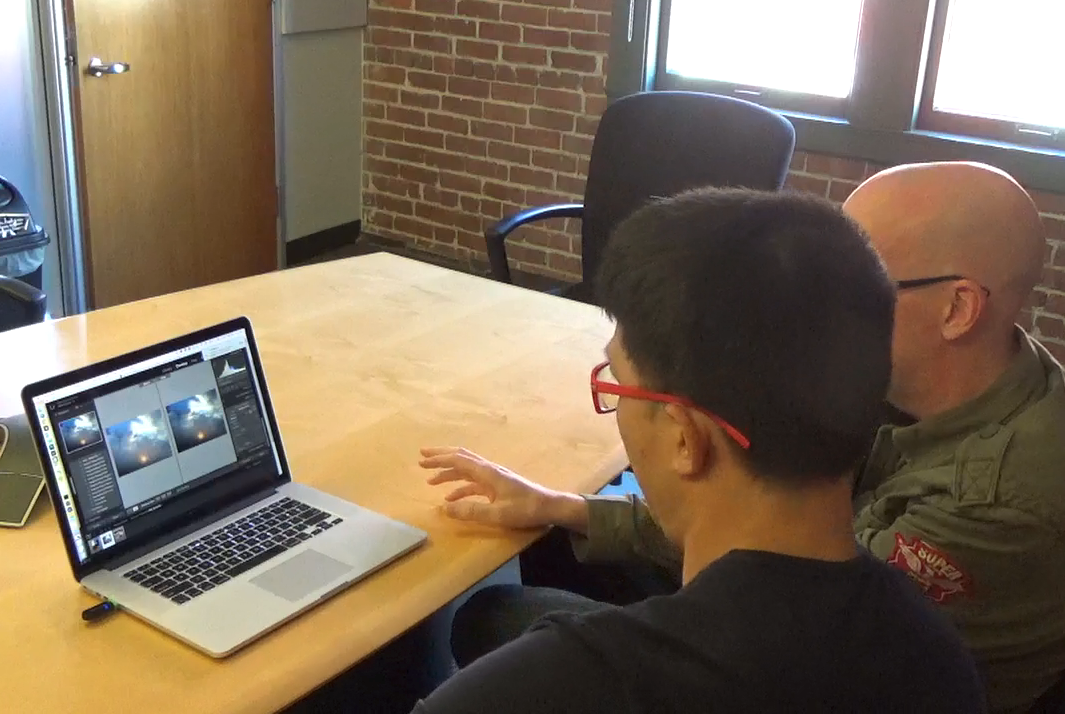
\includegraphics[width=0.6\textwidth]{discoveryspace/figures/obs.png}
  \caption{A novice-expert session. The expert (right) compares the edited photo with the original to illustrate what the edits did.}~\label{fig:discoveryspace_obs}
\end{figure}

\section{Design Goals}
Presenting suggestions relevant to the user's goal can help them accomplish it, as the experts did. Presenting suggestions the user might not have otherwise thought of can help them to discover what is possible and achieve creative results. Combining these insights with prior recommendation research (\textit{e.g.} [12,13,15,20]), we developed five main \textbf{design goals} for suggestion interfaces:
\begin{enumerate}
    \item \textit{Help users get started}: Make suggestions available as soon as the user begins a task. A frequent observation throughout our formative study and prototyping process was that users often did not know where to start in Photoshop.
    \item \textit{Use human language}: Allow users to search using goal terminology, and describe suggestions in a language novices can understand by including a descriptive non-technical title for each. This reflects the growing popularity of natural language or ``semantic'' search [13].
    \item \textit{Show previews} of what a suggestion does, and allow users to easily compare before and after, for example as in Side Views [32].
    \item \textit{Offer faceted browsing} in addition to search to help users explore. This is a well-documented concept in the information retrieval literature (\textit{e.g.}, [12,15,33]), and we believe it to be applicable to software applications as well.
    \item \textit{Suggestions should be relevant} to the user's current task, but should also alert the user to new or unknown possibilities. CommunityCommands users were found to prefer ``contextual'' suggestions related to their short-term history [20], and users of complex software often desire the ability to discover new features [24].
\end{enumerate}

We iterated on the Discovery\-Space design based on feed-back from users with varying levels of Photoshop proficiency. Because Discovery\-Space harvested actions from multiple online sources, they had widely varying amounts of user interaction: some automatically applied effects, while others paused at key points with dialogs for user interaction. We removed such pauses and dialogs when present because they tended to lack sufficient accompanying explanation, and therefore confused some non-expert pilot testers. Users often desired basic adjustments such as brightness/contrast, exposure, and saturation. The actions in our collection generally comprised several steps rather than just one, and so did not include many of these basic edits. We manually created 11 actions for these basic adjustments, which would simply initialize the values to auto, and leave the sliders visible for the user to adjust as they wish.
\section{DiscoverySpace: Action Suggestions}
This section describes the Discovery\-Space interface (\autoref{fig:discoveryspace_interface}) and its keyword-based suggestion algorithm.

\begin{figure}[b!]
\centering
  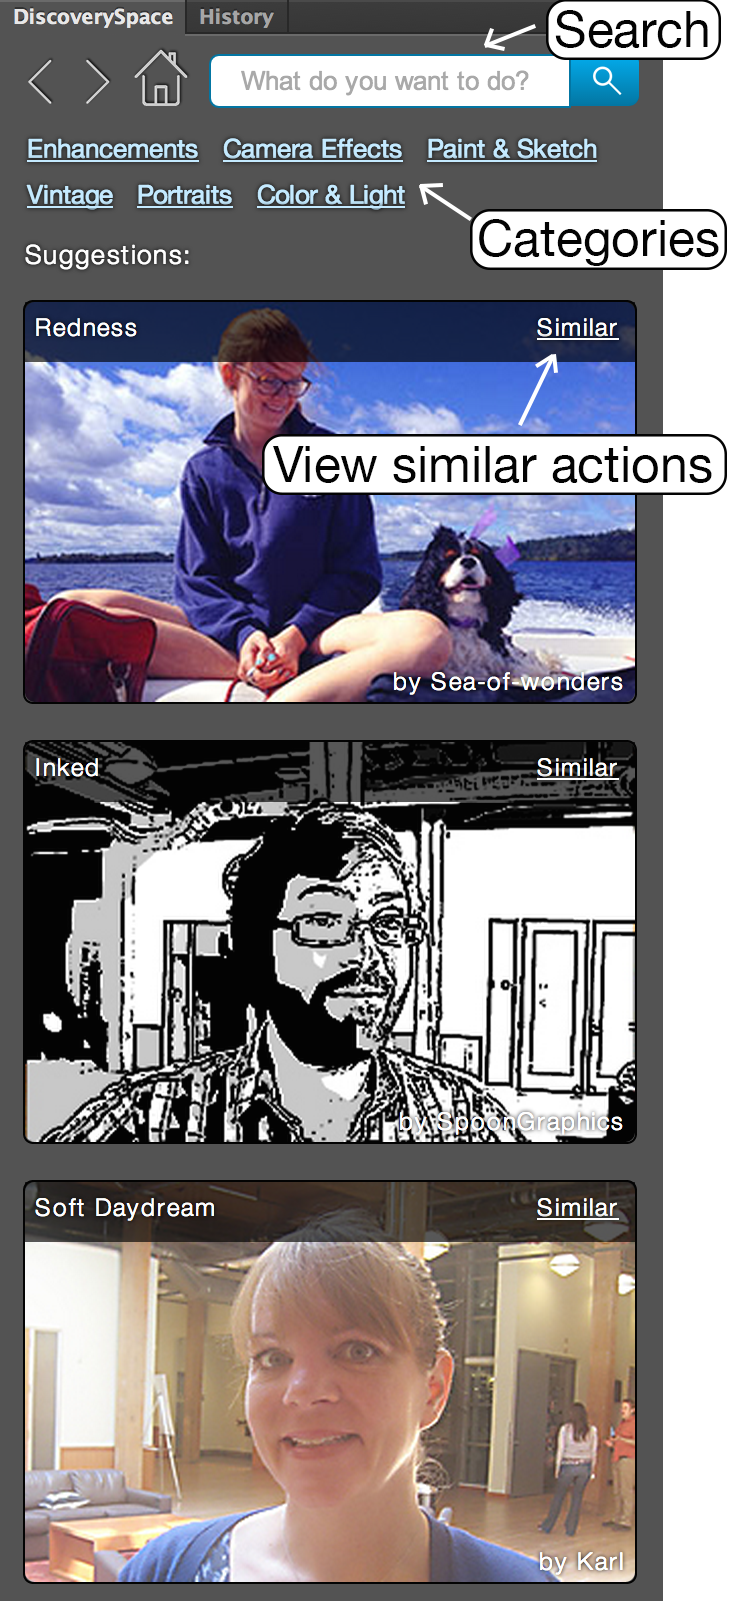
\includegraphics[width=0.35\textwidth]{discoveryspace/figures/discoveryspace_with_labels.png}
  \caption{DiscoverySpace as a panel in Photoshop. Users can apply a suggested action by clicking on its image.}~\label{fig:discoveryspace_interface}
\end{figure}

\subsection{User Experience}
When a user first opens a photo, Discovery\-Space prompts them to enter a goal and select features their image contains from a list (\textit{e.g.} ``contains people'', ``outdoor''). Next, the Discovery\-Space home page appears, containing a search bar, category buttons, and suggested effects (\autoref{fig:discoveryspace_interface}). Each suggestion is displayed by showing the effect applied to an example image with appropriate content. For example, the image for a ``skin smoothing'' effect is of a close-up face. The user can mouse over the image to compare \textit{before} and \textit{after}. Clicking a suggestion applies that action to the photo. As given, the user has no control over the settings for each step of the action; they can see the sequence of steps that was done after applying it by opening the History panel (\autoref{fig:discoveryspace_history}), but cannot step through it or adjust the parameters of individual operations. These actions are therefore intended to allow users to quickly achieve an effect without needing to manually complete all of the intermediate steps. The user can easily undo or redo the effect once it has been applied. If the user scrolls down on the main page, more suggestions appear. To browse suggested effects in a specific category, the user can click a category button. To search the corpus of effects, the user can enter a query in the search bar. The user can also browse effects that are similar to a selected effect by clicking the ``\textit{Similar}'' button on the effect. 

\begin{figure}[b!]
\centering
  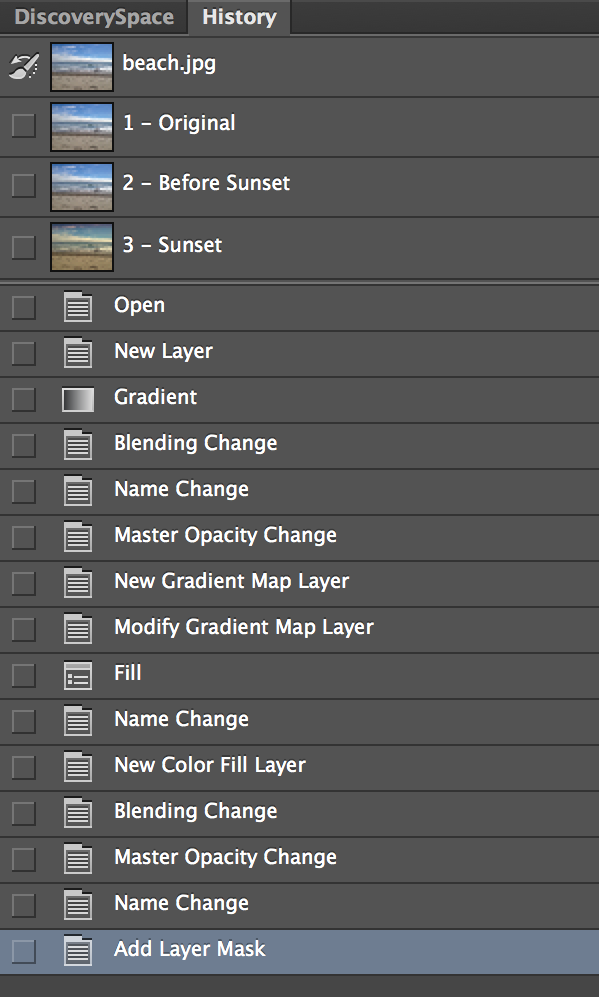
\includegraphics[width=0.35\textwidth]{discoveryspace/figures/history.png}
  \caption{In the History panel, users can review the operations an action has performed.}~\label{fig:discoveryspace_history}
\end{figure}

\subsection{Implementation}
Discovery\-Space is a Photoshop extension panel, written in HTML, Javascript, and Adobe ExtendScript. It retrieves a manually-curated corpus of 115 actions stored on an Amazon S3 server, providing the flexibility to update the actions to reflect popular trends. We manually defined the action categories by reviewing and clustering free actions found online. We created the corpus by downloading 2-3 actions from each subcategory. Paid actions could be added in the future by allowing users the option to pay for effects from within the panel. Discovery\-Space automatically augments search queries with synonyms to maximize the number of relevant results.

\subsection{Keyword-based Recommendations}
Discovery\-Space recommendations take the user's photo as input (\autoref{fig:discoveryspace_rec_alg}). Each action has been assigned a number of descriptive keywords. When opening a new photo, users must select features that describe the image; image analysis could automate this step in the future. We map the selected features to potentially relevant keywords, and assign each action a weight based on the number of matching keywords.

\begin{figure}[b!]
\centering
  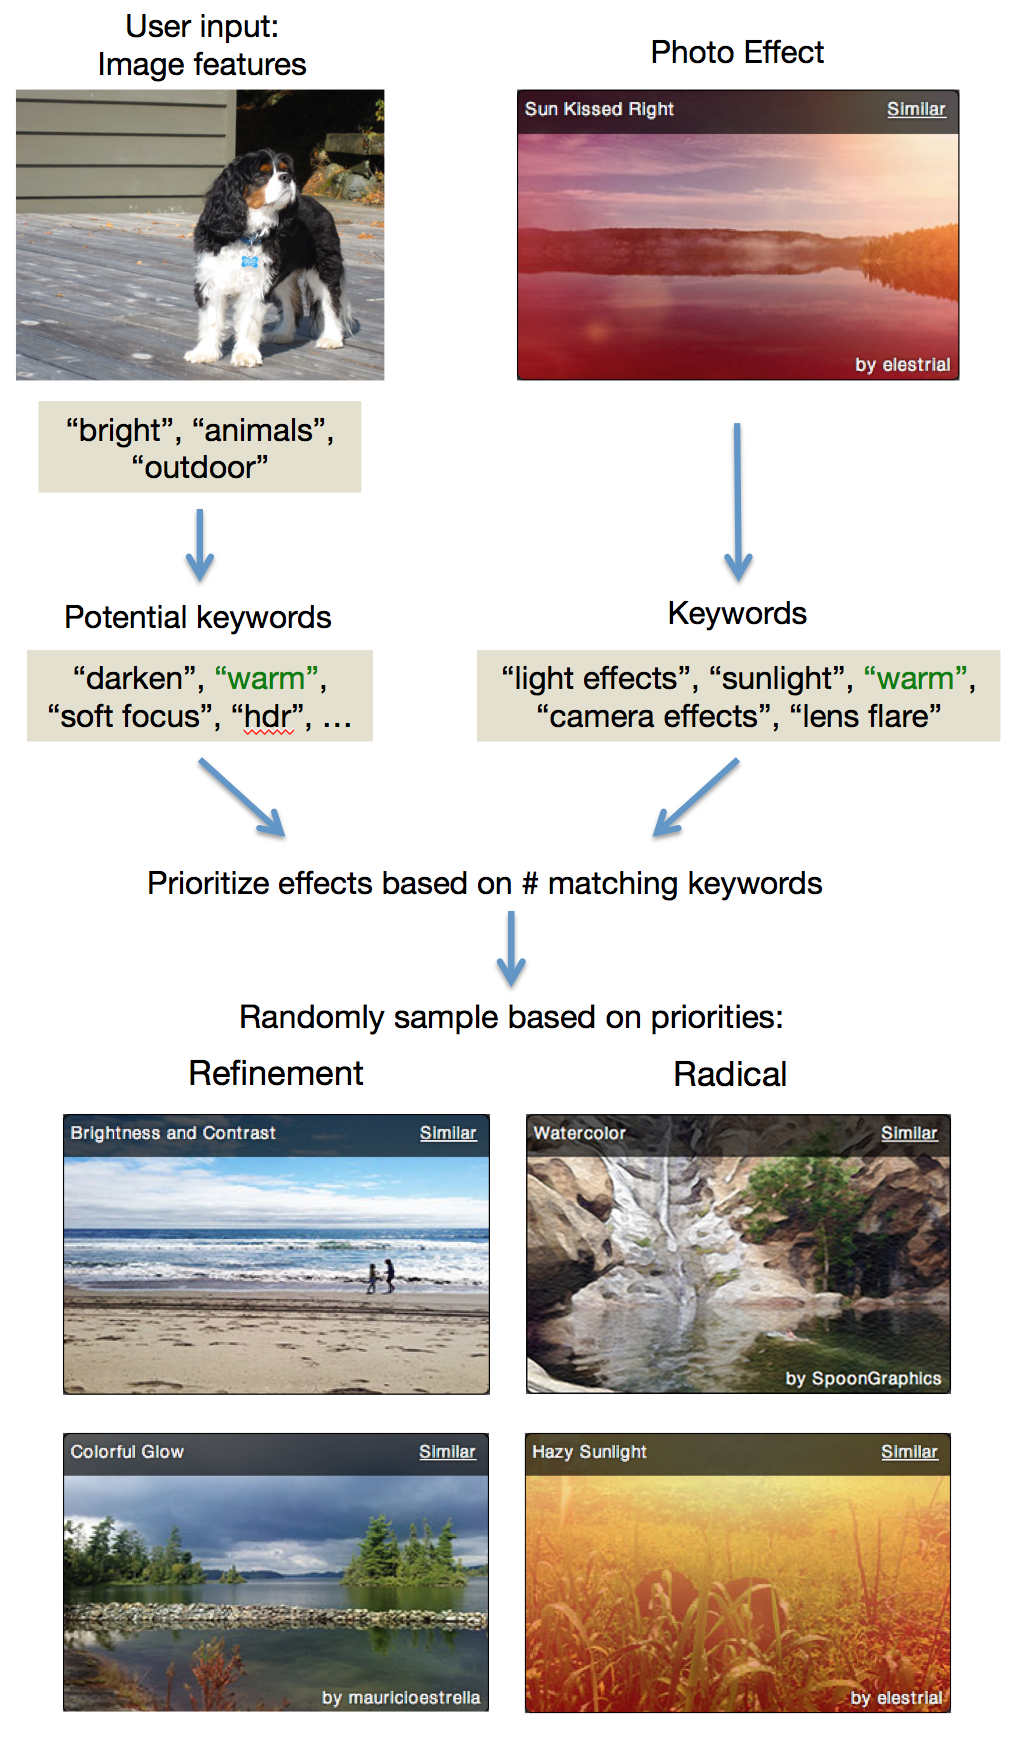
\includegraphics[width=0.6\textwidth]{discoveryspace/figures/rec_alg_new.png}
  \caption{An overview of our keyword-based recommendation algorithm. User-selected image features are mapped to keywords and matched against the keywords for each action in the corpus.}~\label{fig:discoveryspace_rec_alg}
\end{figure}

To select and present suggestions, our algorithm randomly samples from the collection of actions based on these weights: actions with a larger weight have a higher probability of being selected. The randomness encourages discovery by presenting new suggestions when the user refreshes the page. Each action has also been manually classified as either \textit{refinement} or \textit{radical}. An action is deemed \textit{radical} if it produces a drastic effect, does not necessarily maintain realism, and/or takes multiple steps to accomplish. Examples include painting effects, HDR, replicating old cameras, and drastic color effects. An action is deemed a \textit{refinement} if it involves a small adjustment that is meant to improve the photo while maintaining realism, or could be accomplished in one step. Examples include brightening, softening skin, sharpening, and slight color casts. We prefer that both types of effects are suggested, to promote variety in the options. To ensure this, we run the prioritization algorithm separately on the two collections of actions, and then, for every four actions that are suggested, we sample two from the refinement pool and two from the radical pool. This is because on a 27-inch desktop display, Discovery\-Space in its default position shows four suggestions at a time.

\section{Study}
To investigate the efficacy of action suggestions, we conducted a between-subjects experiment in which participants edited their own photos in Photoshop. In the experimental condition, subjects had access to Discovery\-Space; in the control condition they did not. We hypothesized that participants exposed to the suggestions in Discovery\-Space would find the editing process easier, feel more creative, and become more confident using Photoshop. 

\subsection{Method}
To sign up, participants completed a brief initial survey about their Photoshop experience. Participants were then scheduled for a 30-minute session and assigned to one of two conditions: participants in the Discovery\-Space condition used Photoshop with the Discovery\-Space panel open, and participants in the Control condition used Photoshop with a blank panel that instructed them to save their photo when finished (\autoref{fig:discoveryspace_exp_interface}). The study held constant the length of the session (30 minutes), the number of photos edited (two), the questions participants answered when opening and closing a photo, and the availability of a web browser (yes). 

Each session comprised the following steps: consent form, background questions, edit first photo, edit second photo, short interview, and final online survey. The background questions allowed participants to elaborate on their initial survey responses regarding their prior experience with Photoshop and photo editing. Participants were instructed to bring one photo containing at least one person, and one photo without people, to ensure some consistency across participants' photos. The editing order of the two photos was randomly assigned with balancing in each condition. We chose to allow participants to bring their own photos, rather than provide sample photos, so that participants would be more likely to come up with their own goals for their photos, and would be motivated to do a good job. 

\begin{figure}
\centering
  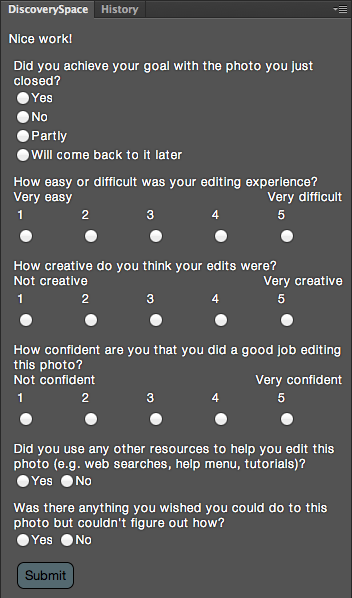
\includegraphics[width=0.6\textwidth]{discoveryspace/figures/close_questions.png}
  \caption{Questions answered by participants after editing each photo. The measure for ``How confident are you that you did a good job editing this photo?'' is referred to as ``confidence about performance'' in the Results.}~\label{fig:discoveryspace_close}
\end{figure}

In both conditions, upon opening a photo, the study panel prompted the user to describe their goal for the photo and select its image features. The panel also prompted the user to answer a few questions about their editing experience every time a photo was closed (\autoref{fig:discoveryspace_close}). The panel was in a prominent location and the participants were made aware of it by the experimenter. The task was open-ended: participants could define their goal however they wanted and were simply instructed to work until they were satisfied (or until time ran out).  We used an open-ended task as opposed to a more directed one because participants would be more likely to perform as they would in a real-world setting when working on personally meaningful tasks. In the Discovery\-Space condition, participants were given a quick overview of the Discovery\-Space interface and were shown what each button in the panel did, so that time would not be wasted figuring out how to use the interface. The History panel was located behind Discovery\-Space, and was only visible when clicked on. Participants in the Discovery\-Space condition were shown the History panel only if they asked explicitly how to go back in time by more than one action. 

In both conditions, a web browser was open on the Google home page just behind Photoshop; participants were told they could use it at any time. This was included to reflect the ready availability of web resources in creative workflows. A short interview and final survey took place in the last five minutes of the session. It comprised follow-up questions on the participant's overall editing experience and their perceived difficulties. 

\subsection{Participants}
28 students were recruited from four undergraduate classes at a Southern California university (one photography class, three design classes). None of these classes provided formal training in Photoshop, though many participants had experience with other photo editing software and/or basic photography principles. Stratified randomization was used to balance gender and Photoshop expertise across conditions. Expertise with Photoshop was measured as follows: in the initial survey, participants were asked to rate their skill level with Photoshop from 1 to 5, and their amount of experience with Photoshop from 1 to 5. The answers to these two questions were added together to produce a score between 2 and 10, and participants were grouped according to their score into Beginner (2-4), Intermediate (5-7) and Expert (8-10). See \autoref{table:ds_participants} for the distribution of participants' expertise and gender. 15 participants were assigned to the Discovery\-Space condition, and 13 to the Control condition (the uneven balance was due to the stratified randomization).

\begin{table}[]
\centering
\begin{tabular}{l|lll}
 & Female & Male & \textbf{Total} \\ \hline
Beginner & 6 & 5 & \textbf{11} \\
Intermediate & 3 & 9 & \textbf{12} \\
Expert & 1 & 4 & \textbf{5} \\
\textbf{Total} & \textbf{10} & \textbf{18} & \textbf{28}
\end{tabular}
\caption{Participants' gender and Photoshop expertise. ALL TABLE CAPTIONS MUST GO ABOVE}~\label{table:ds_participants}
\end{table}

\begin{figure}
\centering
  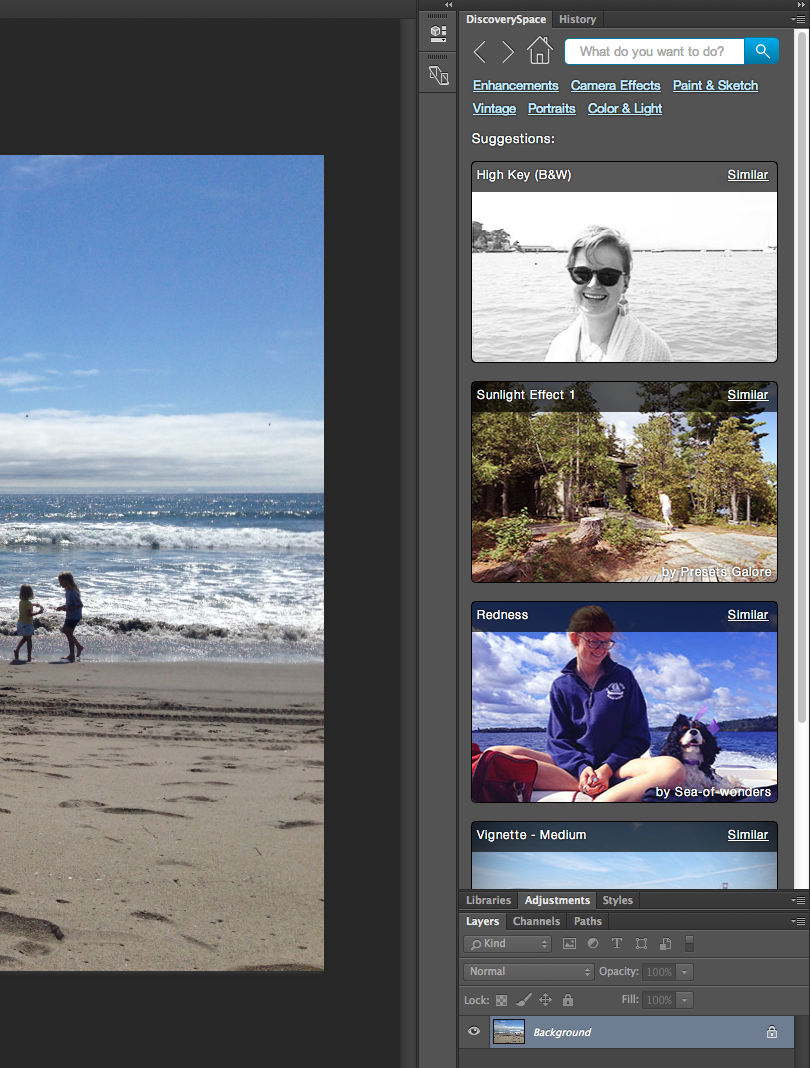
\includegraphics[width=0.4\textwidth]{discoveryspace/figures/experiment-DS.png}
  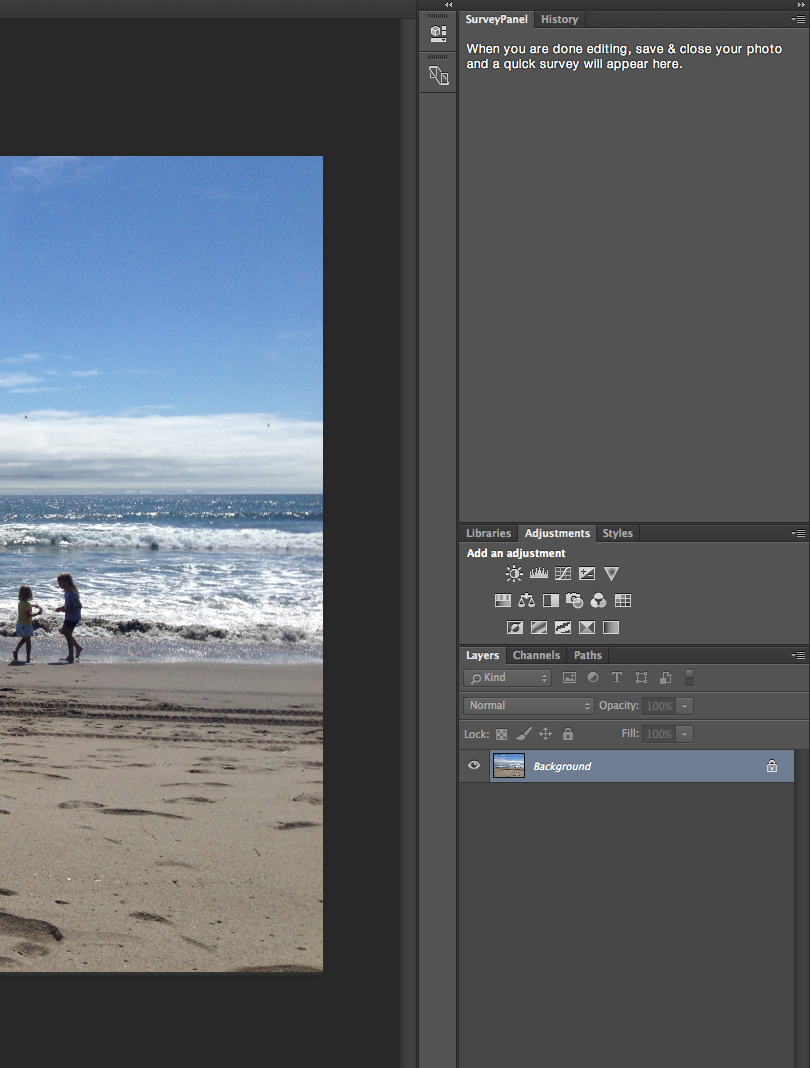
\includegraphics[width=0.4\textwidth]{discoveryspace/figures/experiment-C.png}
  \caption{Photoshop as it appeared in the DiscoverySpace condition (left) and Control condition (right).}~\label{fig:discoveryspace_exp_interface}
\end{figure}

\subsection{Measures}
Both surveys asked participants to rate their Photoshop confidence by answering two questions: ``How confident are you with your ability to edit photos in Photoshop? (1-5)'' and ``How confident are you that you can achieve your goals in Photoshop? (1-5)''. We measured change in confidence as the difference between the sum of both responses (between 2 and 10) in the final survey and the initial survey. For each of the three Likert-scale questions answered after every photo (\autoref{fig:discoveryspace_close}), we added the responses from both photos to obtain one score between 2 and 10 for each participant ($N = 28$). For the questions with yes/no answers, we considered each photo separately ($N = 56$ as each participant edited two photos). We also recorded the number of Photoshop tools used (not including those from Discovery\-Space) and all clicks and pages loaded in Discovery\-Space.

\subsection{Results}
For the numerical measures, we used analysis of variance to analyze Condition, Expertise, and their interaction. For yes/no measures, we used logistic regression with the same variables. 

\subsubsection{Participant Goals}
As expected with such an open-ended task, there was a large variety of participant goals. The most frequent goals focused on color/brightness (\textit{e.g.}, ``correct exposure and color balance'' or ``experiment with color''), or a particular emotional effect (\textit{e.g.}, ``make it surreal looking'' or ``give a lonely, solemn feel''). As expected, participants more often (72\% of the time) used non-technical terms to describe their goals rather than photography-specific terms such as ``saturation'' and ``sharpness''. This was most prominent among Beginners and Intermediates.

\subsubsection{Quantitative Results}
Beginner participants in particular were significantly more likely to lose confidence in the Control condition ($M = -2.0$) and gain confidence in the Discovery\-Space condition ($M = 0.5$), $t(22) = -2.16, p = 0.04$ (\autoref{fig:discoveryspace_confidence}). Across all Expertise levels, Discovery\-Space had only a marginal effect on participants' confidence: the confidence of Control participants decreased ($M = -0.77$) while the confidence of Discovery\-Space participants increased ($M = 0.27$), but this was not significant, $F(1, 22) = 2.97, p = 0.10$. No effect was found for Expertise. 

\begin{figure}
\centering
  \includegraphics[width=0.6\textwidth]{discoveryspace/figures/confidence-new.png}
  \caption{Confidence of Beginner Control participants decreased while confidence of Beginner Discovery\-Space participants increased. Error bars show 1 standard error from the mean. Note that due to small sample sizes in the sub-conditions, this is intended only as a descriptive illustration.}~\label{fig:discoveryspace_confidence}
\end{figure}

\begin{table}[]
\centering
\begin{tabular}{l|l|l|l}
 & DiscoverySpace & Control & $p$ \\ \hline
\textbf{Total confidence change (-8 – 8)} & \textbf{0.27} & \textbf{-0.77} & \textbf{0.10} \\
\textbf{Couldn’t figure something out = yes} & \textbf{50\%} & \textbf{80\%} & \textbf{0.02} \\
Achieved goal = yes & 47\% & 31\% & 0.72 \\
Used web browser & 33\% & 54\% & 0.26 \\
Difficulty (2 – 10) & 5.3 & 6.0 & 0.37 \\
Creativity (2 – 10) & 4.5 & 4.1 & 0.86 \\
Confidence about performance (2 – 10) & 5.9 & 5.2 & 0.68 \\
\# Photoshop tools used & 15 & 20 & 0.38
\end{tabular}
\caption{Summary of mean values for measures compared between conditions. Discovery\-Space participants had marginally \textit{higher} confidence change (this effect was significant within the Beginner group), and stated they could not figure something out \textit{less often} than Control participants.}~\label{table:ds_results}
\end{table}

Discovery\-Space participants were significantly less likely to state that there was something they couldn't figure out ($M = 50\%$) than Control participants ($M = 80\%$), $\chi^2(1) = 5.52, p = 0.02$. 

All measures compared between conditions are summarized in \autoref{table:ds_results}. Responses to many of the post-editing questions varied widely. Within the Beginner group, Discovery\-Space participants rated difficulty as marginally but not significantly lower ($M = 5.3$) than Control participants ($M = 6.8$), $t(22) = 1.62, p = 0.12$. 

Across both conditions, Experts rated difficulty significantly lower ($M = 4.4$) when compared against Intermediates ($M = 5.8$) and Beginners ($M = 6.0$) together, $t(22) = -2.14, p = 0.04$. Experts also used significantly more tools ($M = 26$) than Intermediates ($M = 16$) and Beginners ($M = 16$), $t(22) = 2.37, p = 0.03$. In the Discovery\-Space condition, 51\% of the actions used were radical and 49\% were refinement, which suggests both types of actions were useful.

Overall, there was a strong negative correlation between difficulty and confidence about performance, $r(28) = -.70, p < .0001$. Interestingly, there was also a strong positive correlation between creativity and confidence about performance, $r(28) = .67, p < .0001$.  This effect seems to hold most strongly for Beginners, as the correlation was weaker for Intermediates and Experts only, $r(17) = 0.48, p = 0.05$. Further exploration revealed that using the web was negatively correlated with achieving one's goal, $\chi^2(1) = 8.09, p = .005$, and positively correlated with having trouble figuring something out, $\chi^2(1) = 6.93, p = 0.01$.

Preliminary analyses found no effects for type of class (photography vs. design), so this was excluded from further analyses. Gender was confounded with Expertise (\autoref{table:ds_participants}) so Gender was also excluded from analyses; however within the Beginner group where Gender was roughly balanced, no Gender effects were found.

\subsubsection{Qualitative Results}
Participants were asked at the end of the session if they had discovered any new effects or tools. All Discovery\-Space participants replied yes, most of them adding that Discovery\-Space had exposed them to effects they had not seen before. 9 of 13 Control participants also responded yes, that they had discovered a new tool, mainly by clicking around or from an online tutorial. Two added that while they had discovered a new tool, they were unsure how to use it.

Discovery\-Space participants were asked two additional questions about the kinds of tasks for which they might use Discovery\-Space, and about the capabilities they wish it had. The most popular response to the task question was ``for making quick and fun edits'', such as preparing a photo to post on social media or editing personal photos for fun, as opposed to aiming for professional-looking or detailed edits. The capabilities most participants wished Discovery\-Space had were more control over the result of an effect, such as sliders to dial it down or to adjust its parameters; and the ability to apply the effect to a selected part of the image only. Other requests included an explanation as to how the effect was achieved so that the user could easily repeat it and experiment with it, and better interaction with the document history. Though users could go back and forward through the applied operations using the History panel, it is separate from Discovery\-Space, and does not allow editing of the previous steps.

Discovery\-Space participants were also given the opportunity to share their general thoughts about the panel. Most stated either that they found it helpful, or that it had the potential to be helpful if some of the aforementioned improvements were made. Novice participants in particular seemed on the whole excited by Discovery\-Space as it meant they were able to achieve effects they otherwise would not have thought possible.

\section{Discussion}
Despite the relatively small sample sizes when participants are broken up into sub-conditions, our results suggest that action suggestions can be beneficial for novice users of complex software. Further research should explore these possible effects in more detail.

It may not be that surprising that the confidence levels of participants in the Control condition dropped after using Photoshop. Novice participants were quickly frustrated with the time it took to find functionality and get accustomed to the interface, and more experienced participants struggled to locate forgotten tools and commands. We believe that Discovery\-Space, while it may not currently support all possible goals, provided a friendlier starting point that showed or reminded participants what types of edits are possible. Again, it is not that surprising that this effect was more pronounced for Beginners, as they are the most likely to misjudge their abilities, having never or rarely used Photoshop.

We assume that participants who answered ``no'' to the question, ``Was there anything you wished you could do to this photo but couldn't figure out how?'' were able to accomplish the tasks they set out to do. Participants who answered ``yes'' to the question were prompted to describe what they could not figure out. Most responses named a task the participant had been trying to accomplish (\textit{e.g.}, removing redness from a person's face), but either gave up on or ran out of time. It is likely that Discovery\-Space provided quicker ways to accomplish many of these tasks, and thus participants in the Discovery\-Space condition were more likely to complete them in the time allotted than those in the Control condition. 

As the study involved using the full Photoshop interface, expertise had a great impact on user performance. Observations during the sessions confirmed that Expert users were comfortable with Photoshop's interface, whereas Beginners tended to find it overwhelming because of the large number of menus and buttons. Ratings of creativity and confidence about performance varied widely, likely because the task was open-ended, and these measures depended on each individual's goal. 
The correlation between confidence in performance and creativity indicates that participants in both conditions did tend to include creativity as a criterion for doing a good job, supporting the motivation for an interface that encourages creative exploration. Participants who used the web achieved their goals less often, likely because these are users who had more trouble with their tasks and turned to the web for help. However, using the web did not in fact seem to help them. The following section provides some suggestions as to why that may be.

\subsection{Common Difficulties}
The same researcher conducted all 28 sessions, and observed participants' recurring errors and difficulties. The most prominent observations, outlined here, support our motivation for action suggestions, and provide directions for future work.

\subsubsection{1. Failing to find the best way to accomplish a task}
Several participants used Google to search for help and often followed the top result without realizing that there was an easier, more efficient, or more effective way to accomplish the task. For example, the automatically generated Google summary listed at the top for ``how to crop photoshop'' suggests using the Rectangular Marquee tool, rather than the more relevant Crop tool. In addition, many tutorials included screenshots from older versions of Photoshop, making it difficult for participants to find the tools mentioned. Version-specific help is a challenge for all software. Systems for augmenting search queries with the user's context could improve this (\textit{e.g.} [4]). For example, the top search result shown when ``cc 2015'' is appended to the above Google search is recent and demonstrates the Crop tool. Such functionality could be helpful for Discovery\-Space's search feature when a larger corpus of actions or tutorials is added.

\subsubsection{2. Not noticing when commands cause state changes or side effects}
A common issue participants ran into was creating new layers without realizing, and then having the wrong layer selected when trying to apply another effect. For example, performing an adjustment from the Adjustments panel creates a new Adjustment layer, but does not explicitly notify the user of this. Most actions in Discovery\-Space also create at least one layer. In this study, many participants in both conditions struggled with having the wrong layer selected when trying to apply other edits, which meant those edits did not work as expected. This is an instance of a more general problem in complex software: commands often have side effects that the user is not aware of, which may cause confusion later on. This suggests that programs should 1) make the user aware of what they are doing, and 2) encourage better development of a correct mental model of the program, so that such side effects are not so surprising when they occur. Support for better interactive history may be an important improvement for Discovery\-Space as it would allow participants to work through and explore the steps that have been completed.

\subsubsection{3. Difficulty finding out what tools do}
For novices, complex software has poor information scent [28]: we observed users sequentially browsing menus, toolbars and panels to find something specific or see what is possible. Even with exhaustive search, Beginners seemed to have difficulty understanding what the buttons and menu items did, given only their names and brief tooltip descriptions. When participants did find the desired tool, they often had trouble figuring out how to use it. Better in-app descriptions and assistance are needed. For example, ToolClips augments tooltips to include media content and detailed information [11]. This is an advanced form of ``speaking navigation'': verbose navigational links that improve information scent. While the current goal of Discovery\-Space was to move away from individual tools toward better task-level support, one way to improve information scent for tools could be to display example tasks that a tool is often used for when mousing over it.

\subsection{Study Limitations}
Having an open-ended task facilitated more realistic usage than a pre-defined task, and having participants work on their own personal photos likely increased their motivation to do a good job. However, participants' widely varying goals resulted in widely varying results regarding their editing experience and likelihood of achieving their goals. Future studies might consider more directed tasks to reduce the variability in participants' goals. 

Using self-reported expertise ratings has the potential for inaccurate assignments based on differences in how participants perceive their own skill. Our observations found their self-report sufficiently accurate. However, future studies might consider a more objective expertise measure, such as a pre-test. The pool of ``novices'' is larger than one might think: many Photoshop novices were experienced with photography principles and/or simpler photo editing software. They had domain knowledge, just not expertise on the specific task at hand. Especially with feature-rich software like Photoshop, nearly everyone is a novice in some regard. 

Participants' widely varying expertise levels yielded small sample sizes for measuring interaction effects. However, for this preliminary study, this variety unearthed valuable differences in participant behaviour. 

Finally, many participants ran out of time and stated this as the main reason they could not achieve their goal; future studies should allow participants to work for longer. A longitudinal study would allow for more realistic usage data, as participants could use the application on their own time and more goals could be collected per person. 

\section{Future Work}
Participants' experiences with Discovery\-Space suggest several ways to improve the robustness and usability of action suggestions in complex software.

\subsection{Improving Discovery\-Space for Photo Editing}
An important limitation of the current Discovery\-Space prototype is that most actions in its corpus produce \textit{global} edits, not \textit{local} ones. A few actions intended for faces (\textit{e.g.} skin smoothing) allow the user to brush on the effect, but the majority apply to the entire photo. This is representative of the selection of free Photoshop actions available online; most are global edits because these are much easier to create than ones that allow for user input such as selection. However, users often desire local editing capabilities, and so providing actions that allow for this would be valuable. One way of providing support for user input would be to leverage the interactive steps provided by TappCloud \cite{Laput2012}.

Based on participants' responses to the question of what tasks they would use Discovery\-Space for, it seems to be effective for quick exploration. In order to help users make more professional-looking edits, Discovery\-Space could take better advantage of the properties of the user's input photo and apply effects in a content-adaptive way \cite{Berthouzoz2011} or suggest automatic fixes based on properties of the photo such as its histogram (\textit{e.g.} as in \cite{Bychkovsky2011}). 

Other immediate improvements to Discovery\-Space for photo editing will include automatic image analysis to replace manual user descriptions of photos, and replacing the default preview images of effects with previews of the user's actual photo.

\subsection{General Improvements to Action Suggestions}
Many programs have the capability to record and save actions (\textit{e.g.}, Adobe Photoshop, Illustrator, and Acrobat), also referred to as presets (\textit{e.g.}, Adobe Lightroom), action macros (\textit{e.g.}, Autodesk's AutoCAD), and macros (\textit{e.g.}, Microsoft Excel and Word). Even more programs allow for task automation via scripting (\textit{e.g.}, Adobe InDesign, Mac OS). Discovery\-Space and the following proposed improvements can apply not only to Photoshop but to any complex software that provides some way of combining operations into actions.

\subsubsection{End-user control}
The most frequent piece of feedback received throughout the study and prototyping process was the desire for more control over the effects. One of the main advantages complex programs have over simple ones (\textit{e.g.}, Instagram) is the ability to have fine-grained control over operations, and so providing this control to users would be a valuable component of an interface like Discovery\-Space. This could be accomplished by examining current usage data of the software in question to determine what parameters users most often edit for common operation sequences, and making only those parameters available when an action is executed. Alternatively, Discovery\-Space could make the action history more interactive by allowing users to select, edit, and delete any step that was performed. To provide an intuitive way of setting parameters, visual previews like the variations in Side Views \cite{Terry2002} and TappCloud \cite{Laput2012} could be incorporated. 

\subsubsection{Recommendation algorithm}
Given the diverse goals that users have in complex applications, a technique like collaborative filtering could improve recommendations by personalizing the suggestions to the user and their goals. Li \textit{et al.} recommend an ``item-based'' collaborative filtering algorithm based on their work with CommunityCommands \cite{Li2011}. This algorithm bases recommendations on the similarity between commands, rather than between users. They also found that users preferred recommendations based on their behaviour within the current session, rather than long-term. The goals users enter into Discovery\-Space should also be included as input to the suggestion algorithm, so that suggestions are not only relevant to the user's photo, but also to the goal they have in mind. This natural language description could also be used to annotate the operations executed by users. With this extra information, we could build a better model of the relationships between goals, the language used to express them, and the tools used. Such descriptions would otherwise be difficult to collate, as users would be required to do extra work to describe the operations they perform.

\subsubsection{Building a scalable corpus of actions}
User-generated actions are posted across multiple sites and carry differing amounts of metadata and detail, and differing distribution licenses. Curating our corpus of actions required careful attention to these differences, and we had to manually define keywords and names for most actions. Scaling up such a corpus or building it automatically would require accounting for these issues. This could be done by creating a centralized repository inside the software itself or as part of Discovery\-Space, wherein users can create and share actions, and are required to provide keywords and agree to a distribution license. An existing example of this is AdaptableGIMP, an interface for the photo editor GIMP that provides user-created actions referred to as ``task sets'' \cite{Lafreniere2011}. Users can create and share task sets from within the interface, and search the corpus for ones to apply.

Action suggestions need not be user-created. They could instead be generated by automatically recording and segmenting user behaviour along with the type of document being worked on, or by mining and analyzing the large collection of online tutorials that are available for most applications. Work has been done on generating interactive tutorials from static online ones \cite{Fourney2014Mining, Laput2012}, and incorporating such work into a search and suggestion interface like Discovery\-Space is a promising direction for improving both the initial usability and long-term learnability of complex software applications.

\section{Conclusion}
This paper introduced Discovery\-Space, a task-level action suggestion interface, and found that easy-to-execute task-level action suggestions may help prevent novices from losing confidence with complex software. Discovery\-Space allows users to more easily discover what is possible in an application by abstracting away individual commands in favour of understandable and goal-driven actions. By suggesting actions relevant to the user's input document, Discovery\-Space can provide useful assistance toward accomplishing the user's task. The experiment described in this paper confirmed the need for interventions like this in modern software, and provided results suggestive of the fact that action suggestions are beneficial to users. 

\section{Acknowledgements}
We thank Nancy Reid \& Catherine Hicks for their help with statistical analyses. This work was supported in part by a Powell Fellowship from UC San Diego.
\chapter{CritiqueKit: Interactive Guidance Techniques for Improving Creative Feedback}
\label{chapter:critiquekit}
\begin{quote}
All of the systems presented so far have aimed to support people doing creative tasks in complex software. But with creative tasks, the software is not always the only complex part. Creative tasks can themselves be complex and difficult by virtue of being subjective and open-ended. One example of such a task is giving feedback. Good feedback is critical to creativity and learning, but many people do not know how to actually \textit{provide} effective feedback. This chapter contributes empirical evidence that two interactive techniques – reusable suggestions and adaptive guidance – can help people provide better feedback on creative work. We present these techniques embodied in the \textit{CritiqueKit} system to help reviewers give specific, actionable, and justified feedback. Two real-world deployment studies and two controlled experiments with CritiqueKit found that adaptively-presented suggestions improve the quality of feedback from novice reviewers.
\end{quote}

\section{Introduction: Feedback's Hidden Potential}
Feedback is one of the most powerful influences on learning and achievement [14]. Both giving and receiving formative feedback encourage self-reflection and critical thinking on one's work [24,31], especially in creative and open-ended domains such as design and writing [14,35]. The growing scale of many educational and professional settings increases both the importance and difficulty of providing sufficiently descriptive and personalized feedback. Good feedback can be hard to generate, and people are not consistently skilled in doing so [22,46]. Feedback is often too short, vague, and not actionable [20,40,45]. Even experienced reviewers don't always recognize when they are providing poor feedback or why it is ineffective [40].

This paper contributes two interactive techniques that improve feedback, their embodiment in the CritiqueKit system, and their evaluation through two deployments and two experiments.

\textbf{Interactive guidance of feedback characteristics.} CritiqueKit features a guidance panel with checkboxes that update as the reviewer gives feedback. A text classifier categorizes feedback as Specific, Actionable, and/or Justified as the reviewer types, providing them with an ambient awareness of their feedback quality and guiding them to improve their feedback. 

\textbf{Suggesting prior feedback for reuse.} CritiqueKit enables reviewers to reuse expert feedback, reducing experts' labor by scaling their feedback to similar work. These suggestions update and adapt based on the feedback's categorization to give reviewers targeted ideas for how to improve their comment and provide inspiration. 

Two deployment studies and two controlled experiments investigated the efficacy of these interactive techniques on the quality and characteristics of feedback. The first deployment examined how experienced reviewers (teaching assistants) reuse feedback in an undergraduate course. The second deployment examined how undergraduate students reuse feedback. The first experiment examined the impact of statically presented suggestions and interactive guidance on novice feedback. Finally, the second experiment examined the efficacy of adaptively updating suggestions in tandem with interactive guidance on novice feedback. We found that adaptively-presented suggestions improved feedback quality (\autoref{fig:critiquekit_exp2}). Reviewers found suggestions useful for inspiration, and the interactive guidance reminded them to ensure their comments met the criteria for effective feedback. This work provides evidence that interactive techniques such as suggestions and guidance can effectively scaffold the feedback process (See \autoref{table:critiquekit_all_results} for details).

\begin{table}
\centering
  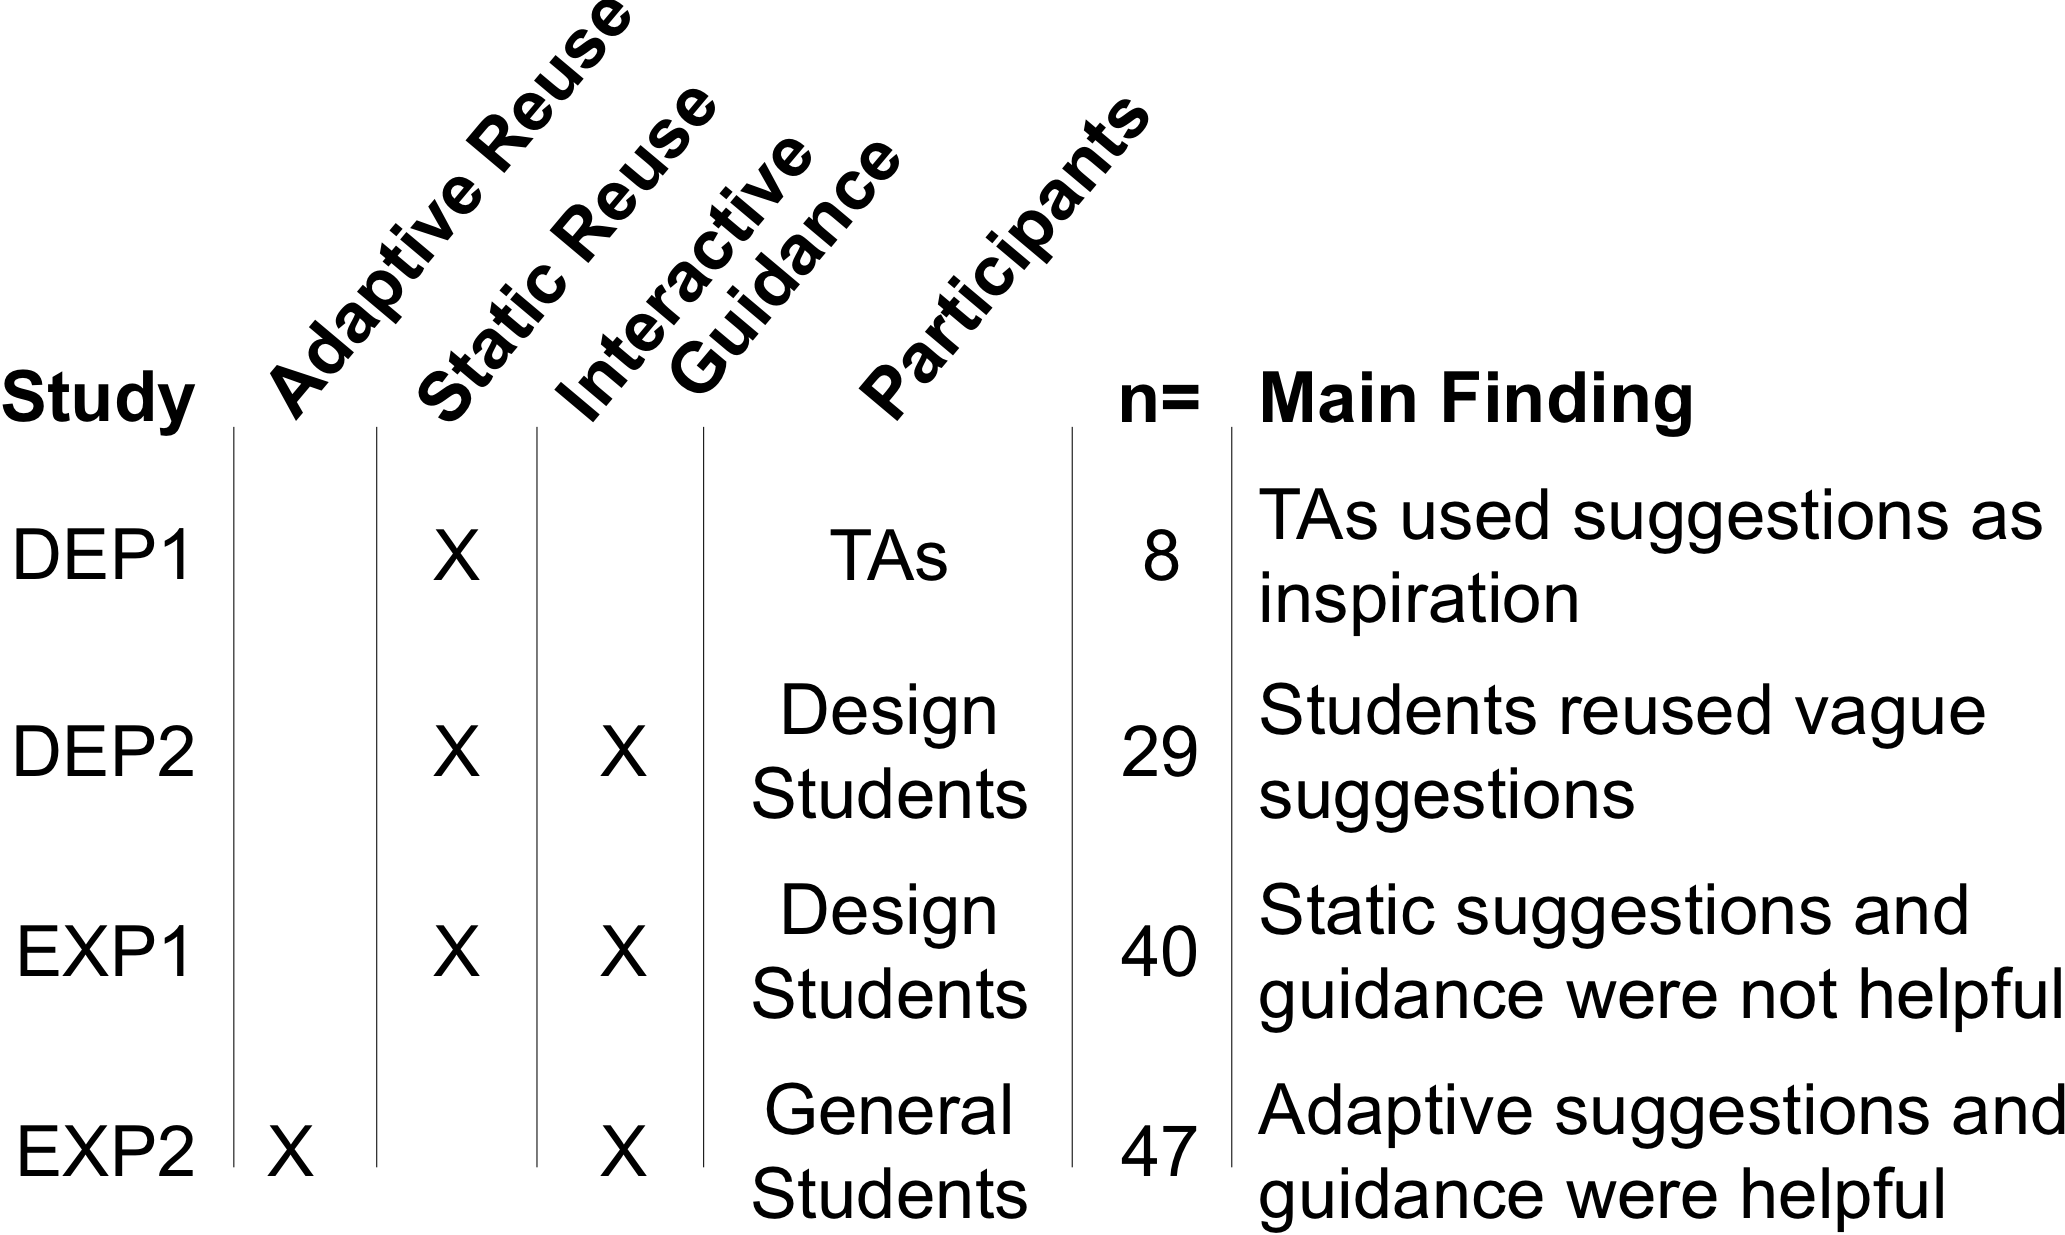
\includegraphics[width=0.6\textwidth]{critiquekit/figures/table1.png}
  \caption{Two deployments (DEP) and two between-subjects experiments (EXP) examined the efficacy of feedback reuse and interactive guidance. We found that interactive suggestions and guidance were most helpful for improving feedback.}~\label{table:critiquekit_all_results}
\end{table}

\section{Related Work}
\subsection{Good Feedback is Actionable, yet Rare}
Rapid iteration is critical to the success of creative projects, from essays, to visual design, to buildings \cite{Dow2010, Sadler1989}. Receiving feedback early on is important for learners to test alternatives and course-correct \cite{Dow2010, Tohidi2006}. Effective feedback is especially important in educational settings where novices are learning new skills and developing expertise. However, giving effective feedback is rarely taught \cite{Nicol2006}. As physical and digital classrooms increase in size, the demand for feedback outgrows the ability to adopt the ideal learning model of one-to-one feedback \cite{Bloom1984}. Instead, a one-to-many approach is utilized, where an expert provides feedback for multiple learners. Although learners most value expert feedback \cite{Gielen2010, Yang2006}, the one-to-many approach is highly demanding on experts, and specific, actionable feedback for individuals becomes increasingly rare. 

In general, effective feedback is specific, actionable, and justified. Specific feedback is direct and related to a particular part of the work rather than vaguely referent \cite{Krause2017, Sadler1989, Yuan2016}. Specific positive feedback also highlights strengths of the work and provides encouragement, so the recipient can tell they are on a good path \cite{Kelley2013, Tseng2007, Yuan2016}. Actionable feedback is important because it offers the learner a concrete step forward \cite{Sadler1989, Sommers1982, Tseng2007, Yuan2016}. Simply pointing out a problem is not sufficient to help one improve \cite{Ramaprasad1983, Sadler1989, Sommers1982, Tohidi2006}. Actionable feedback is often most helpful early in a project \cite{Cho2006, Tseng2007, Yuan2016} because it may help people self-reflect and self-evaluate their work \cite{Gibbs}, prompting more revisions for improvement \cite{Dow2012, Topping1998}. Lastly, justification is an important characteristic of feedback \cite{Krause2017, Narciss2006, Yuan2016}, but is arguably one of the hardest to understand or recognize \cite{Gielen2010}. Justified feedback contains an explanation or reason for a suggested change, which helps the learner understand why the feedback was given.

\subsection{Rubrics \& Examples Usefully Focus Feedback}
Rubrics \cite{Andrade2005, Yuan2016} and comparative examples \cite{Krause2017} are effective in structuring feedback because they beneficially encourage attention to deep and diverse criteria. Novices otherwise tend to focus on the first thing they notice, often surface-level details \cite{Greenberg2015, Hicks2016, Kulkarni2015, Yuan2016}. Viewing examples of past designs can lead to greater creativity and insights \cite{Kulkarni2014, Marsh1996}; thus, showing examples of good feedback may spark ideas reviewers would not have otherwise considered \cite{Greenberg2015, Kulkarni2013, Luther2015}. Also, adaptive examples curated to match design features are more helpful than random examples in improving creative work \cite{Lee2010}. 

Rubrics and other scaffolds require significant upfront manual work by experts who must carefully design a comprehensive rubric, curate a thorough set of examples, or decide how else to structure the feedback process. This chapter investigates leveraging existing feedback to dynamically create rubric criteria. We hypothesize that showing reviewers previously-provided feedback can guide their attention to important aspects of the design. 
\subsection{Is Feedback too Context-specific for Practical Reuse?}
Schön persuasively argues that effective feedback should be context-specific and expert-generated \cite{Schon1983}. He offers a vignette from architecture where the teacher suggests an alternative building to the student as an example of situated wisdom and its transfer. If Schön is right that this exchange requires both wisdom and context, does that mean that feedback reuse is infeasible? Within a given setting, project, or genre, common issues recur. Hewing to the principle of recognition over recall, we hypothesize that suggestions and guidance can increase novices' participation in context-specific exchanges. 

\subsection{Prior Systems \& Approaches for Scaling Feedback}
Existing approaches for scaling personalized feedback include clustering by similarity (\textit{e.g.}, for writing \cite{Brooks2014} and programming \cite{Glassman2015, Head2017}). Gradescope \cite{Singh2017} and Turnitin \cite{Turnitin} allow graders to create reusable rubric items and comments to address common issues and apply them across multiple assignments. Gradescope binds rubric items to scores, which emphasizes grades rather than improvement. 

Other methods include automating the reuse of the solutions of previous learners. These methods work best when correct and incorrect solutions are clearly distinct, such as in programming \cite{Glassman2016Learnersourcing, Hartmann2010} and logical deductions \cite{Fast2013}. Automated methods have also found success with the formal aspects of more open-ended domains such as writing \cite{Brooks2014, Roscoe2014}.  However, assessing the quality and effectiveness of creative work – the strength of a design, the power of a poem – is intrinsically abstract and subjective and lies beyond current automated analysis techniques. Also, little automated analysis exists for media other than text. For domains like design, human-in-the-loop analysis will remain important for quite some time. 

\subsection{Automatically Detecting Feedback Characteristics}
Although feedback is often specific and contextual \cite{Schon1983}, general characteristics can be automatically detected and used to help reviewers improve their feedback. For example, PeerStudio \cite{Kulkarni2015} detects when comments can be improved based on the length of the comment and the number of relevant words. Data mining and natural-language processing techniques can also automatically detect whether a comment is actionable or not, and prompt the reviewer to include a solution \cite{Nguyen2016, Xiong2012}. Krause \textit{et al.} use a natural-language processing model to detect linguistic characteristics of feedback and suggest examples to reviewers to help them improve their comment \cite{Krause2017}. These methods require a reviewer to first submit their comment so it can be analyzed, and then improve their comment after submission.

\section{CritiqueKit: Interactively Guiding Feedback}
Based on these methods and insights, CritiqueKit (\autoref{fig:critiquekit_interface}) categorizes feedback and provides prompts and suggestions to reviewers. It differs from prior work by providing feedback to reviewers as they type rather than after they submit. We hypothesize that this ambient feedback with suggestions may provide a just-in-time scaffold that changes how reviewers' thoughts crystallize, yielding feedback that is more specific, actionable, and/or justified. 

\begin{figure}[b!]
\centering
  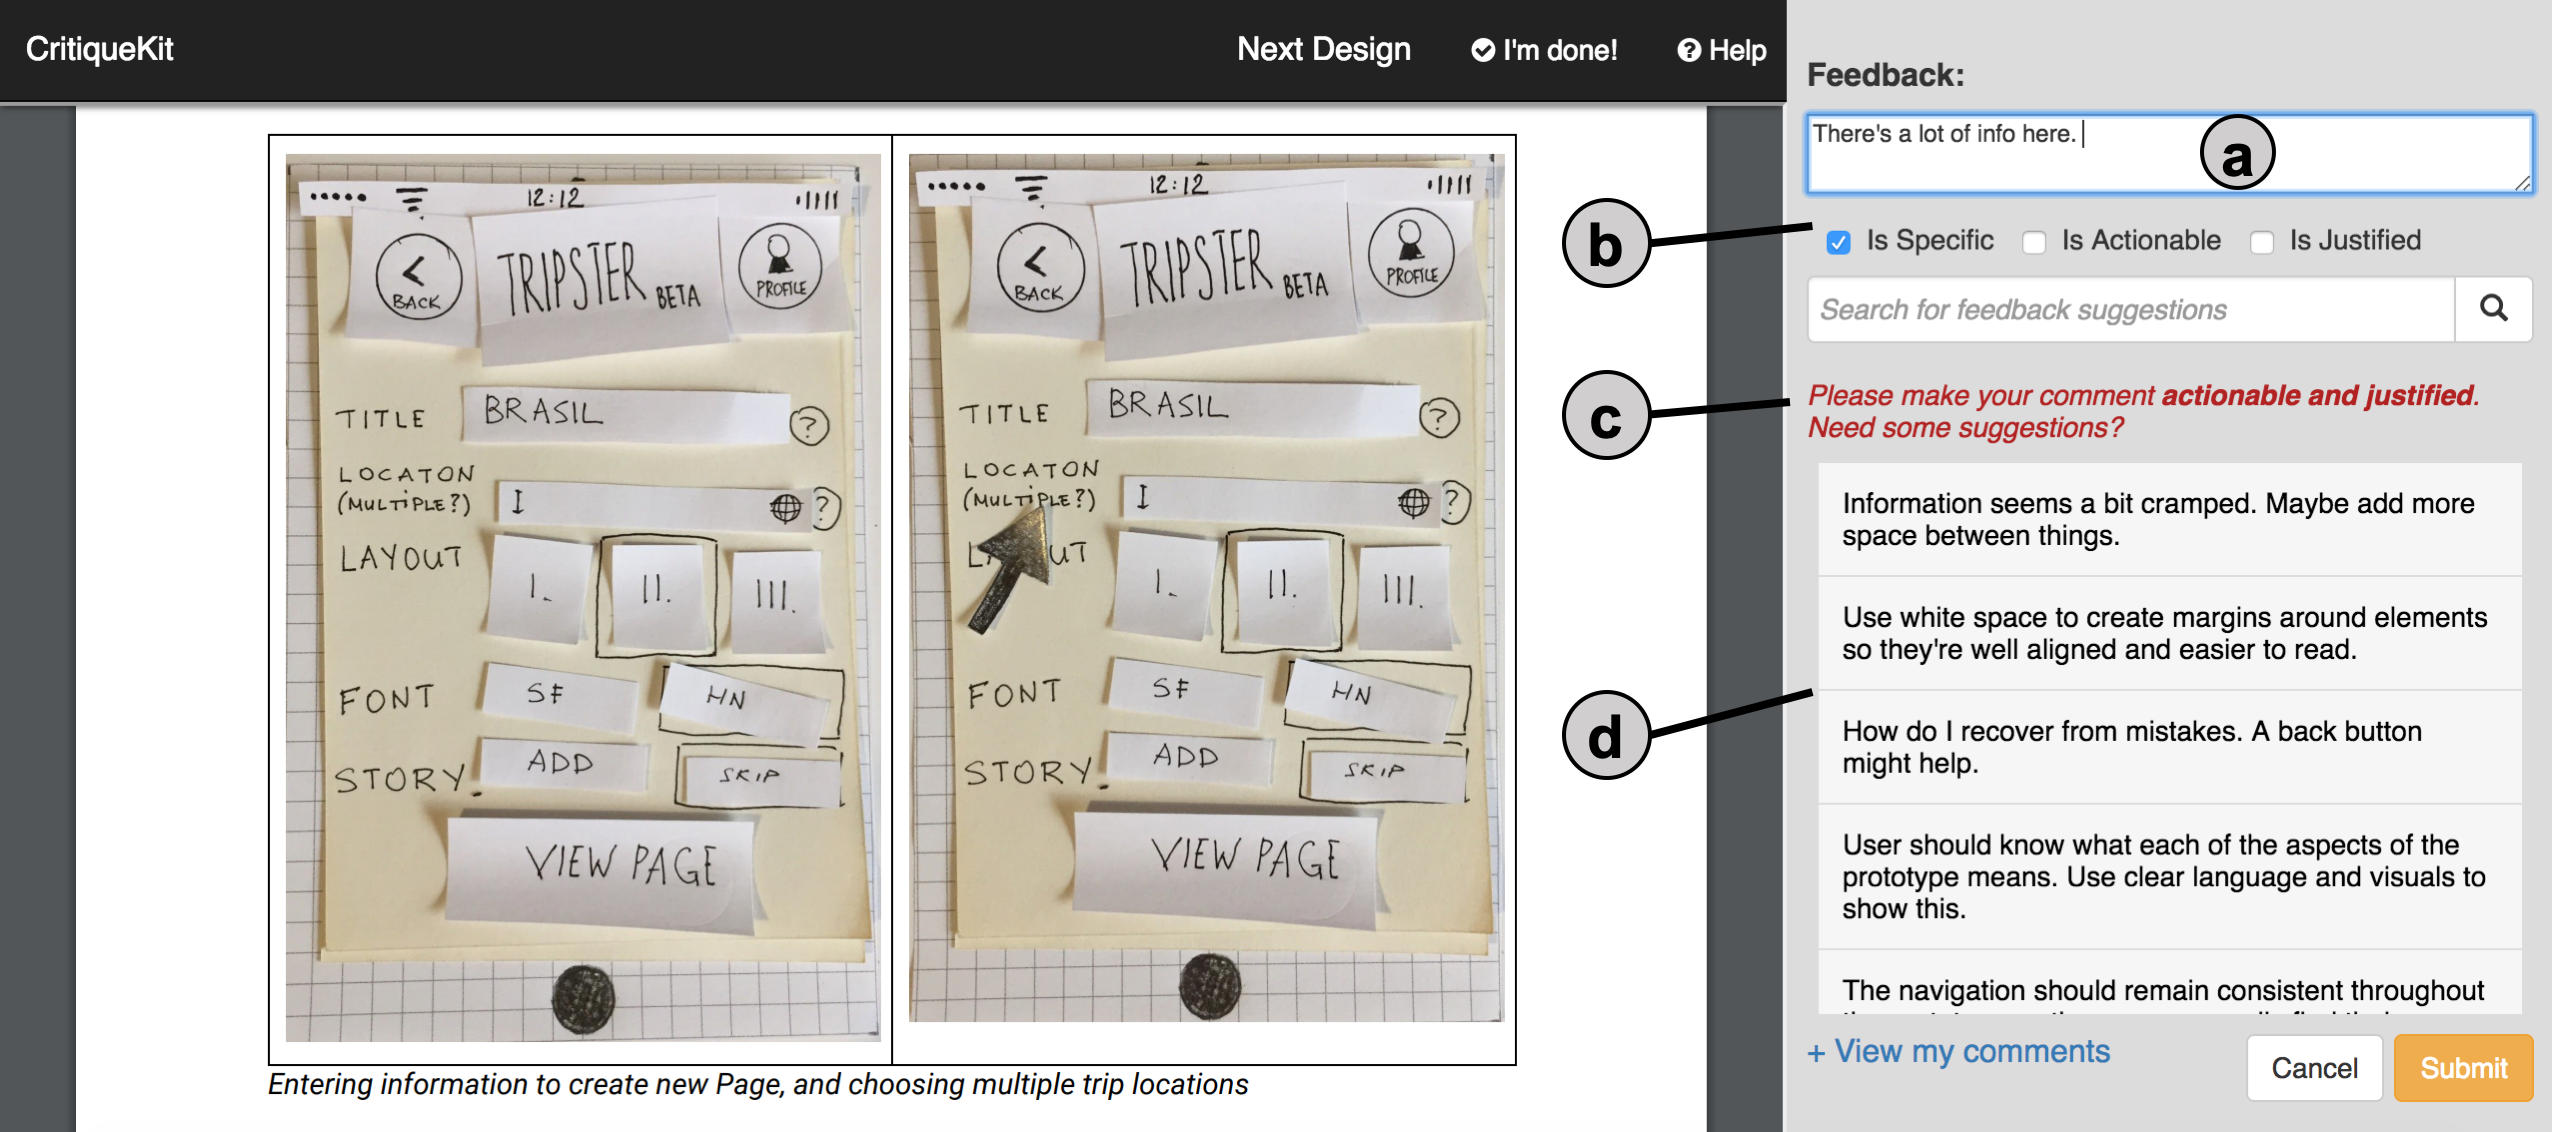
\includegraphics[width=\textwidth]{critiquekit/figures/interface.png}
  \caption[The final CritiqueKit interface for EXP 2.]{The final CritiqueKit interface for EXP 2. a) The reviewer can type their feedback in the textbox. b) The checkboxes in the guidance panel update based on the characteristics of the reviewer’s comments. c) CritiqueKit explicitly prompts reviewers to ensure their comment fits the checkboxes in the guidance panel. d) The reusable feedback suggestions in the suggestions box update based on the unchecked characteristics in the guidance panel, adapting the suggestions specifically to the reviewer's feedback.}~\label{fig:critiquekit_interface}
\end{figure}

\subsection{Interactive Guidance as a Form of Scaffolding}
CritiqueKit features an interactive guidance panel (\autoref{fig:critiquekit_interface}b) with checkboxes that update based on which of three attribute categories the feedback fits: \textit{Is Specific} \cite{Krause2017, Sadler1989, Sommers1982, Yuan2016}, \textit{Is Actionable} \cite{Dow2012, Gibbs, Kulkarni2015, Luther2015, Sadler1989, Tseng2007}, and \textit{Is Justified} \cite{Gielen2010, Krause2017, Narciss2006, Yuan2016}. 

The prototype assesses the feedback's fit with the following heuristics. The heuristic for the \textit{specific} category merely requires that comments be at least five words long because vague comments tend to be short, such as ``good job'' or ``needs work.'' Perhaps surprisingly, we observed that the five-word nudge was sufficient to garner specific feedback in practice. (Some websites, like Etsy, also use a five-word minimum heuristic for reviews). For the \textit{actionable} and \textit{justified} categories, we manually combed feedback that had been hand-labeled as meeting these categories and observed that specific keywords (i.e., ``maybe try'' and ``you should'' for actionable; ``because'' and ``so that'' for justified) were strong cues of these features. Consequently, the prototype implementation simply checks for the presence of these keywords and phrases in feedback comments. 

A comment is considered complete once all checkboxes are checked. Reviewers can manually check and uncheck the checkboxes if they feel the checkboxes did or did not add a category in error. For example, if a reviewer's comment states, ``Use a 2-column grid layout,'' and the ``Is Actionable'' checkbox remains unchecked, the reviewer can manually check the checkbox to note that their comment does indeed contain an actionable suggestion. 

\subsection{Adaptive Suggestions for Greater Specificity}
The suggestions box (\autoref{fig:critiquekit_interface}d) contains a list of previously given feedback from experts. These suggestions dynamically adapt based on how the reviewer's feedback is categorized in the guidance panel. For example, if a reviewer's comment does not yet satisfy the actionable and justified categories (as in \autoref{fig:critiquekit_interface}), the suggestions box would contain examples of feedback with these characteristics. Suggestions appear in the order they were added to the corpus.

\subsection{The CritiqueKit Review Workflow}
When a reviewer first opens CritiqueKit, a prompt asks them to provide specific feedback on something they like about the design and something that could be improved. The suggestions box contains general feedback snippets \cite{Kulkarni2013} pertinent to the review criteria to give reviewers a starting point, providing suggestions that are broadly applicable and fit within the specified criteria. The ``Submit'' button at the bottom of the interface is red to indicate that the comment text box is either empty or does not fit any of the categories in the guidance panel. 

Once a comment is sufficiently long, the ``Is Specific'' checkbox will check, and the reviewer will be prompted to make their comment actionable and justified. The ``Submit'' button turns yellow to indicate that their feedback is not yet complete, though they can still submit if desired. The feedback suggestions then change to present comments that instantiate both actionable and justified feedback. The suggestions continue to adapt depending on the characteristics of the comment, showing reusable examples of feedback that satisfy the unchecked categories in the guidance panel. Once all checkboxes are checked, the ``Submit'' button turns green as an indication of completeness. 

Using prior feedback as suggestions can give inspiration and highlight common issues. The presence of the structured guidance panel reminds reviewers of attributes that feedback should have. 

\subsection{Implementation}
CritiqueKit is a client-server web application implemented using Node.js; it assumes that all content to be reviewed is available on the web. The corpus of reusable feedback comments is stored on the server in JSON format.

CritiqueKit uses web sockets for communication between each client running the app and the main server, implemented using the socket.io module. Feedback classification happens on the client-side using JavaScript. Feedback suggestions are also generated on the client-side after retrieving the corpus from the server; the suggestions box adaptively shows and hides comments using JavaScript. 

Users access CritiqueKit by navigating to its URL in a web browser. The first time the browser loads the website, a unique ID is generated for the user and sent to the server. A cookie is also saved on the client-side so that the server can identify and differentiate users. The review content is loaded within the page as an iframe.

\section{Deployments: (How) Is Feedback Reused?}
To understand how feedback is reused in educational settings and evaluate the CritiqueKit approach, we conducted two deployments and two experiments. All studies took place at a research university. 

\subsection{DEP 1: How Do Teaching Assistants Reuse Feedback?}
Eight teaching assistants (TAs) (two female) for an undergraduate design course used Gradescope to grade and critique seven weekly assignments that varied in content from storyboards to written explanations to high-fidelity web application prototypes. TAs set rubric items for each assignment and wrote comments for each. We deployed CritiqueKit to first understand how TAs might reuse feedback and made iterative improvements to the design throughout the quarter based on TA input.

\begin{figure}[b!]
\centering
  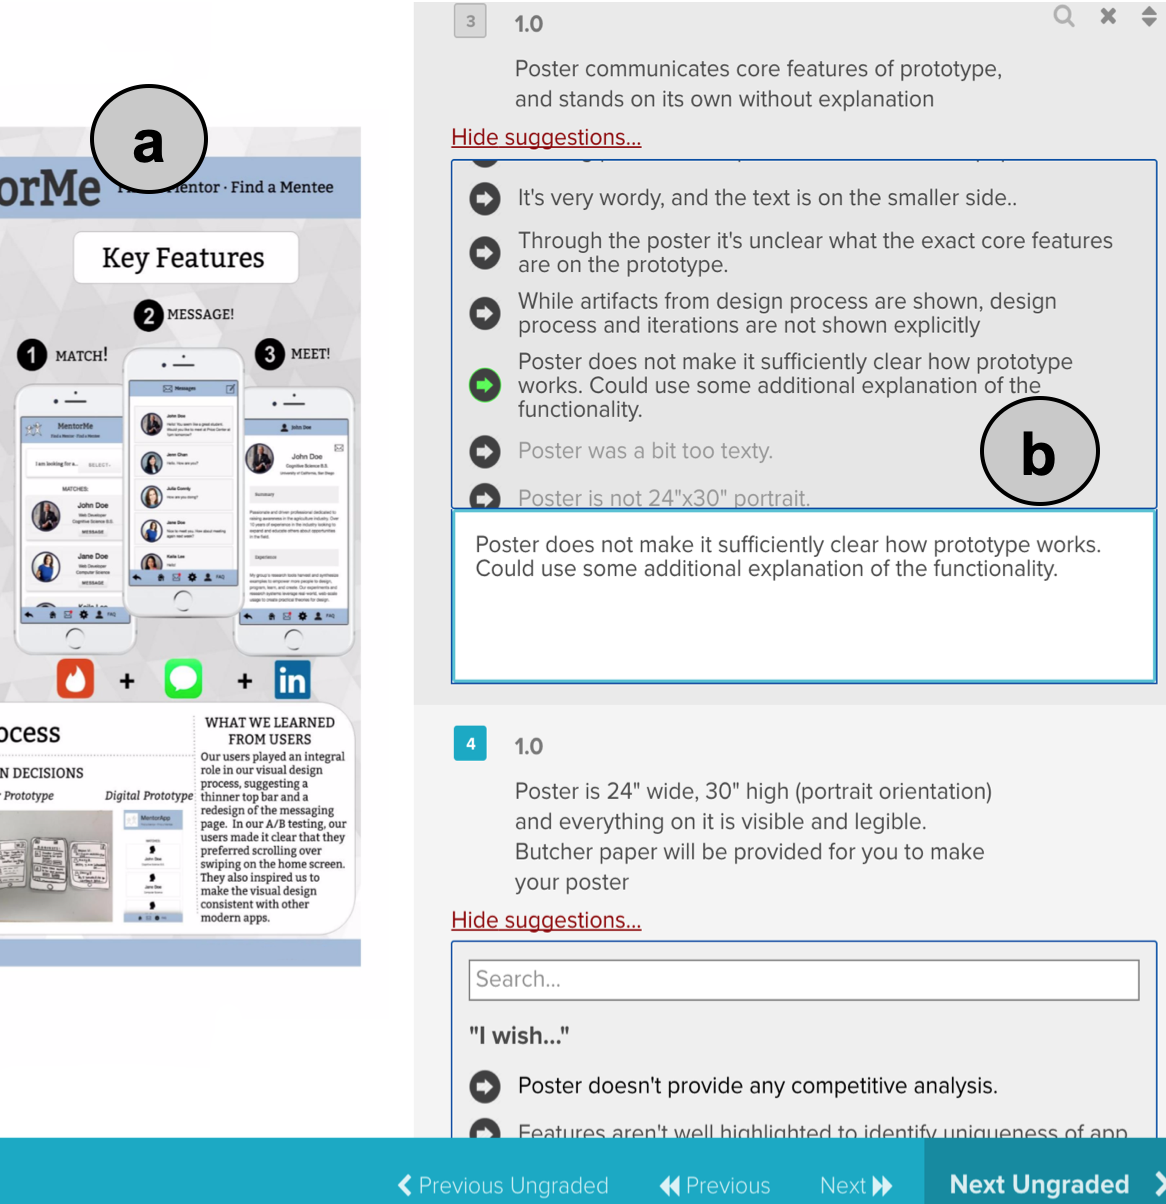
\includegraphics[width=0.6\textwidth]{critiquekit/figures/gradescope.png}
  \caption{CritiqueKit implemented as a browser extension in Gradescope for DEP 1. a) Reviewers provide feedback on a student design. b) The suggestions box under each rubric item provides reviewers with a list of reusable suggestions and a comment box for providing feedback on a submission.}~\label{fig:critiquekit_gradescope}
\end{figure}

\subsubsection{Method: Integrating CritiqueKit with Gradescope}
To integrate with the TAs' existing workflow, we implemented CritiqueKit as a Google Chrome extension that augments the Gradescope interface with a suggestions box (\autoref{fig:critiquekit_gradescope}). This version of CritiqueKit contained only the suggestions box to explore feedback reuse. The suggestions box contained a manually curated set of feedback provided by former TAs in a previous iteration of the course, stored in a Google Sheet online and retrieved by the Chrome extension using the Google Sheets API. Suggestions were categorized into three feedback categories: Positive, Problem, and Solution. TAs could select feedback suggestions to directly copy into the textbox for further editing. Each rubric item contained its own suggestion box interface, providing suggestions specific to that rubric item.

We curated the reusable suggestions corpus as follows. Given all feedback from the previous quarter, feedback that was 25 or fewer words in length was kept, because longer feedback was both too long to be skimmed in a suggestion display and tended to be overly specific. Feedback of 26-30 words was truncated at the sentence level to fit within the 25-word limit. Longer comments or duplicate comments were discarded. In total, 526 comments were provided as suggestions throughout the course for seven (of ten) assignments. Suggestions were manually categorized into the Positive ($n = 92$), Problem ($n = 312$), and Solution ($n = 122$) categories.

\subsubsection{Result: TAs Used Feedback Suggestions as Inspiration}
Across seven assignments, four of the eight TAs reused 51 distinct suggestions from the 526-element corpus (9.7\%). 75 of 583 designs received a reused suggestion for feedback. 60\% of reused suggestions were categorized in the Problem category. These numbers omit any reuse occurring entirely inside Gradescope without CritiqueKit. (Gradescope provides an interface for reusing entire comments within an assignment rather than for individual parts of the comment.) 

An end-of-course survey asked TAs about their CritiqueKit use. One commented that he would ``\textit{skim the comments in the [suggestions] to see if something was accurate to my thoughts}.'' Another mentioned that the prototype helped him ``\textit{[find] ways to better explain and give feedback about specific points}.'' TAs also mentioned that suggestions sometimes reminded them to comment on more diverse aspects of students' work. For example, one mentioned that seeing positive suggestions reminded her to give positive feedback, not only critiquing areas for improvement. TAs mentioned using the suggestions as inspiration rather than the exact wording, taking the underlying concept of a suggestion and tailoring it.

\subsection{DEP 2: How Do Students Reuse Feedback?}
The first deployment examined teaching staff usage; this second deployment examined student usage to understand how novices interact with guidance and suggestions. We deployed CritiqueKit as a standalone web application with 29 students in an undergraduate design course for five weeks. Students gave anonymous feedback on two randomly assigned peer submissions for each of seven assignments.

\begin{figure}[b!]
\centering
  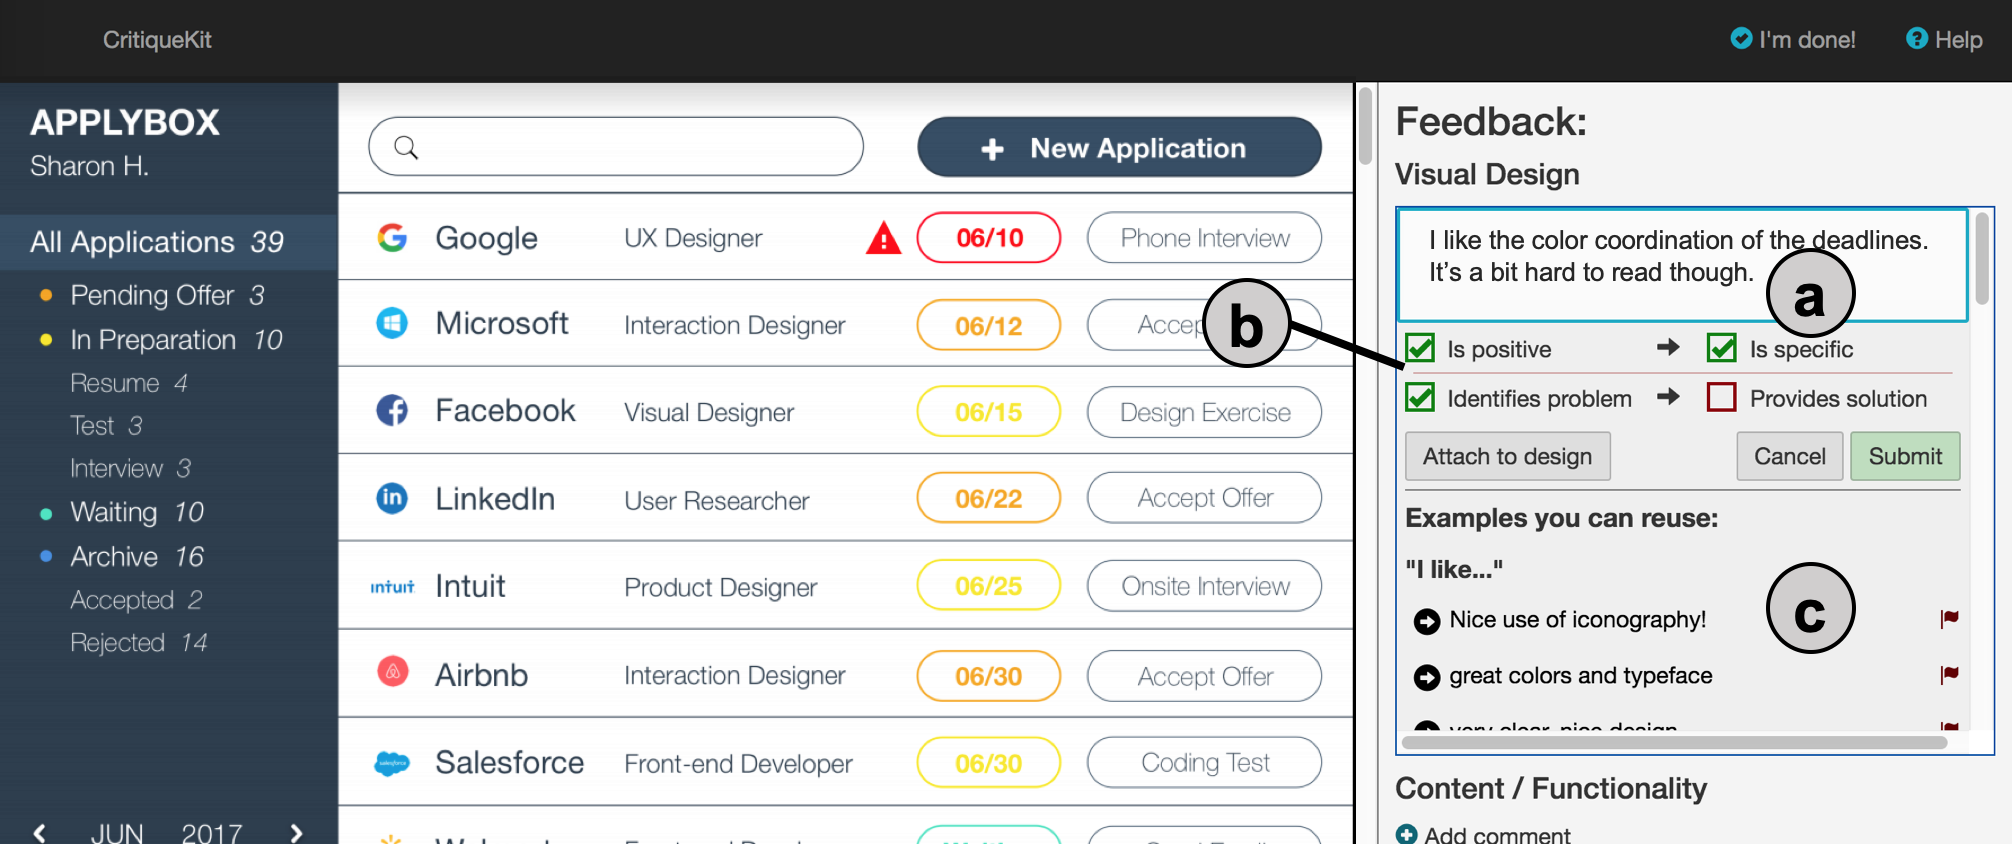
\includegraphics[width=\textwidth]{critiquekit/figures/old_interface.png}
  \caption[The CritiqueKit user interface for DEP 2 and EXP 1.]{The CritiqueKit user interface for DEP 2 and EXP 1. a) The reviewer types their feedback into the text box. b) Checkboxes in the guidance panel update as the reviewer types to show how well the comment fulfills high-quality feedback criteria. c) The reviewer can browse and reuse previously given feedback.}~\label{fig:critiquekit_exp1}
\end{figure}

\subsubsection{Method: Integrating Interactive Guidance for Scaffolding}
Novice students are less experienced in giving feedback and may benefit from interactive scaffolding \cite{Reiser2004}. This version of CritiqueKit included an interactive guidance panel to help reviewers provide more specific and actionable feedback (\autoref{fig:critiquekit_exp1}). The categories on the guidance panel were ``Is Positive,'' ``Is Specific,'' ``Identifies a Problem,'' and ``Presents a Solution'' with checkboxes next to each. These categories stem from recommendations in the literature for both positive and critical feedback \cite{Kelley2013}. Similar to the final version of CritiqueKit, these checkboxes updated as a reviewer typed by classifying their comment into the three categories. The categories differed from the final version, focusing on specific and actionable feedback. 

The suggestions box was seeded with feedback from the course TA. Similar to the first deployment, the suggestions were categorized in the Positive, Problem, and Solution categories. When a student submitted a comment, it was classified into one of these categories, shortened to 25 words if it was longer, and fed back into the corpus to appear as a suggestion, enabling students to reuse their peers' as well as their own comments. The suggestions were ordered first by frequency used, then by shortest length first, and updated as these values changed and more comments were added. Compared to the final version of CritiqueKit, suggestions were static, meaning they did not change as the reviewer typed.

\subsubsection{Results: Positive Feedback Common; Reuse Rare}
For seven assignments, 898 comments were submitted. Independent raters classified each comment into the five categories of Positive Only, Positive  and  Specific (Positive + Specific), Problem Only, Solution Only, and Problem with a Solution (Problem + Solution). 45\% of these comments contained positive feedback; 30\% contained a Problem + Solution statement. 

Students rarely selected feedback suggestions for reuse. Over the five-week deployment, 14 distinct suggestions were reused on 27 student designs for four of the seven assignments. These suggestions were mostly short, vague comments such as ``I wish this was more visually appealing.'' This may be because students often left feedback specific to individual designs that did not easily generalize to other contexts. Students' comments in a post-survey confirmed that the suggestions did not always seem applicable. Students also did not regularly use the interactive guidance panel; 15 of the 29 students engaged with the panel a total of 120 times over five weeks. 

In contrast to how TAs reused feedback, students may not have recognized common issues. TAs paid attention to common errors between designs and mainly reused Problem feedback, whereas students may not have noticed or attended to underlying issues between designs. For instance, one student mentioned that they did not use the feedback suggestions because they ``\textit{rarely pointed out the same things when critiquing interfaces}.'' 

This exploratory deployment investigated how students reuse feedback and respond to interactive guidance in the classroom. To understand how a system with these features compares to a standard feedback system, the next study was a controlled between-subjects experiment. 

\section{Experiments: Scaffolding Feedback}
Following our deployments, we conducted two empirical studies to investigate the impact of suggestions and guidance on feedback quality.

\subsection{EXP 1: Do Static Suggestions Improve Feedback?}
In an online between-subjects study, 40 undergraduate design students were asked to review three restaurant website homepages using CritiqueKit. The task emulated peer review tasks often required in creative courses. This study's suggestion corpus came from a design feedback task on CrowdCrit \cite{Luther2015} and was categorized in the Positive, Problem, and Solution categories. We hypothesized that suggestions and guidance would help reviewers provide more specific and actionable comments.

\subsubsection{Method: Reviewing Restaurant Websites}
40 participants were randomly assigned to either the CritiqueKit condition or the Control condition (20 in each). CritiqueKit participants used the same version of CritiqueKit as DEP 2 with all features available (\autoref{fig:critiquekit_exp1}). Control participants used an otherwise identical version consisting solely of a comment text box. Upon landing on the homepage of either version, participants were provided with a scenario explaining that three restaurant owners are seeking feedback on their new website design. Participants were given a brief tutorial of CritiqueKit's features and an explanation of what makes for good feedback. There were no restrictions or requirements on time spent or amount of feedback to provide. We compared the percentages of comments in five categories. Comments including a supportive element were labeled as \textit{Positive Only} or \textit{Positive + Specific}. Comments including a critical element were labeled \textit{Problem Only}, \textit{Solution Only}, or \textit{Problem + Solution}.

\begin{figure}[b!]
\centering
  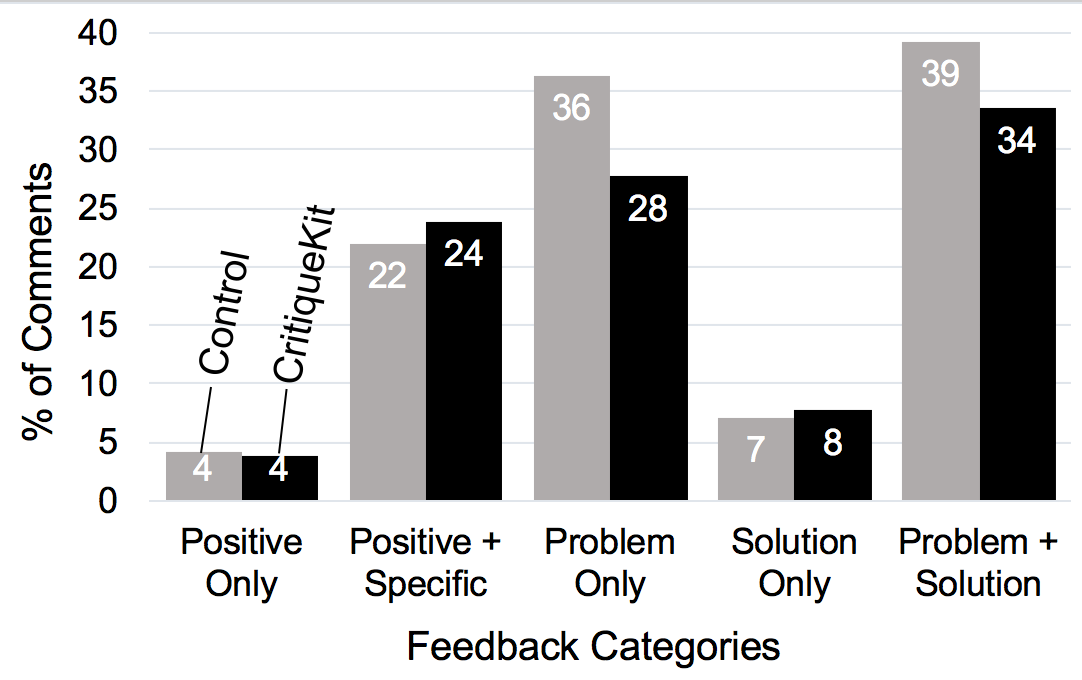
\includegraphics[width=0.6\textwidth]{critiquekit/figures/exp1_feedbacktypes.png}
  \caption{A plurality of feedback in both conditions in EXP 1 identified both a problem and solution (\textit{i.e.}, was actionable). Feedback that was only positive was the rarest. There were no significant differences between conditions for these categories.}~\label{fig:critiquekit_exp1_results}
\end{figure}

\subsubsection{Results: Static Suggestions Were Not Helpful}
With static suggestions and interactive guidance, there were no significant differences between conditions. (To foreshadow, we will see differences in EXP 2, which adds adaptive suggestions). Participants provided a total of 323 comments (168 for control, 155 for CritiqueKit). The average number of words per comment was not significantly different between conditions (Control: $m = 29.07, SD = 23.64$; CritiqueKit: $m = 23.22, SD = 17.3$) ($F(1,38) = 2.52, p = .11$).

\subsubsection{Suggestions \& Guidance Did Not Affect Type of Feedback}
The distribution of the five category types did not vary significantly between conditions ($x^2 = 4.80, df = 4, p = .31$) (\autoref{fig:critiquekit_exp1_results}). In both groups, participants provided mostly Problem + Solution feedback (39\% in Control; 34\% in CritiqueKit). 

\subsubsection{Most CritiqueKit Participants Corrected Category Labels}
65\% of CritiqueKit participants actively used the guidance panel, making a total of 85 corrections to categories. Interaction with the guidance panel may have indicated attention to the feedback characteristics. As the study was online, we don't know how many of the other 35\% were influenced by the guidance panel. 

\subsubsection{Unfortunately, People also Reused Vague Suggestions}
11 distinct suggestions from the corpus were reused. 8 of these were vague; 3 were specific. 15 of 155 reviews included a reused suggestion. This seems especially low given the high engagement with the guidance panel. We see two reasons for this: First, the suggestions came from CrowdCrit \cite{Luther2015}, where participants provided feedback on a weather app design. The study task was different than the task for which the suggested feedback was originally given, and novices may have had a limited ability to see the deep structure behind a suggestion and reapply it in a new context. Second, the suggestions were created by crowd workers and of uneven quality. 

The suggestions selected were typically short, positive comments, perhaps because students did not know how to apply them in the specific context. For example, the most commonly reused suggestion was ``great use of color'' (reused 3 times). This result is similar to DEP2 in which students did not find feedback provided by other peers or novices to be useful and generalizable. Feedback suggestions may require more curation or quality control to be most useful. 

\subsubsection{Suggestions \& Guidance Should Work in Concert}
While this version of CritiqueKit contained both feedback suggestions and interactive guidance, these features functioned independently. Regardless of the categories checked in the guidance panel, the suggestions remained static and presented in the same order for each participant, potentially making them easy to ignore if they were irrelevant to the context. Participants may have paid attention to only one feature at a time. The next study investigated the question of whether adaptively presenting feedback suggestions along with interactive guidance improves feedback. 

\subsection{EXP 2: Do Adaptive Suggestions Help?}
The second experiment used the final version of CritiqueKit described in the system section to test the hypothesis that adaptively-presented suggestions combined with guidance would improve feedback by increasing the fraction of feedback that is specific, actionable, and/or justified.

\subsubsection{Method: Reviewing Paper Prototypes}
We conducted a between-subjects in-person study with 47 (27 female) participants. Participants were recruited from an undergraduate subject pool within the Psychology and Cognitive Science departments. Participants were randomly assigned to either the CritiqueKit ($n = 24$) or Control ($n = 23$) conditions. 44 of these participants had no design course experience; 3 participants had taken at least one design course. 28 spoke English as a second language. 

Participants were asked to provide feedback on two designs from students enrolled in an online course who volunteered to receive more feedback on their work. These designs were PDFs of mobile application paper prototypes. The review criteria included whether the prototype supported the student's point of view and whether it seemed easily navigable. Participants were first shown the design instructions and review criteria and then given a short tutorial of CritiqueKit as well as an explanation of what makes for good feedback. CritiqueKit participants had all features of CritiqueKit available to them (\autoref{fig:critiquekit_interface}), while Control participants used a version that consisted of only a textbox for their feedback. The task took about 30 minutes to complete. After providing feedback on both designs, participants were interviewed about their feedback process and use of CritiqueKit. 

\subsubsection{Presenting Feedback Suggestions Adaptively}
The categories on the guidance panel and their definition used for coding participants' responses were the following:\\
\textbf{Specific}: relates directly to the review criteria\\
\textbf{Actionable}: gives a concrete suggestion for improvement\\
\textbf{Justified}: provides a reason for why something is done well or should be improved

For DEP 2 and EXP 1, the guidance panel categories sought to encourage specific and actionable feedback (\autoref{fig:critiquekit_exp1}). Examining the feedback from our previous studies, we found that ``Is Positive'' and ``Identifies a Problem'' did not provide significant guidance as reviewers were generally aware of whether their feedback was positive or critical. In addition, the guidance panel did not explicitly check for justification of feedback. For EXP 2, we revised the categories to ``Is Specific,'' ``Is Actionable,'' and ``Is Justified'' to also encourage the explanation or reasoning behind feedback. As described in the system section, the checkboxes update as the reviewer types to reflect the categories present in their comment, and the suggestions adapt to show feedback examples from categories not yet present in the comment. 

\subsubsection{Results: CritiqueKit Participants Provided More Specific, Actionable, \& Justified Feedback}
Participants provided 158 total comments (79 control, 79 CritiqueKit). The percentage of comments that contained all three categories (specific, actionable, and justified) was significantly higher in the CritiqueKit condition (53\%) than in Control (30\%) ($x^2=8.33, df = 1, p = .01$) (\autoref{fig:critiquekit_exp2}). As an example, this comment meets all three: ``The `more questionnaires' section (Specific) should be made smaller (Actionable) because it is not the main focus of the page.'' (Justified). The system's heuristic for checking specificity of a comment was quite simple: five words or greater in length. Feedback raters blind to each condition used a more sophisticated and holistic assessment, taking specific to also mean related to the review criteria. With this assessment, 98\% of CritiqueKit comments were labeled by raters as specific whereas only 83\% of Control comments were. These raters also rated comments from EXP 1 within the specific, actionable, and justified categories to provide a comparison between the two experiments. Interestingly, the percentage of comments containing all attributes in the Control condition was relatively consistent between EXP 1 (35\%) and EXP 2 (30\%). The percentage of comments with all attributes in the CritiqueKit condition greatly increased between the two experiments (26\% versus 53\%). Having the checkboxes may have explicitly reminded CritiqueKit participants to ensure their comments satisfy the specific, actionable, and justified categories.

\begin{figure}[b!]
\centering
  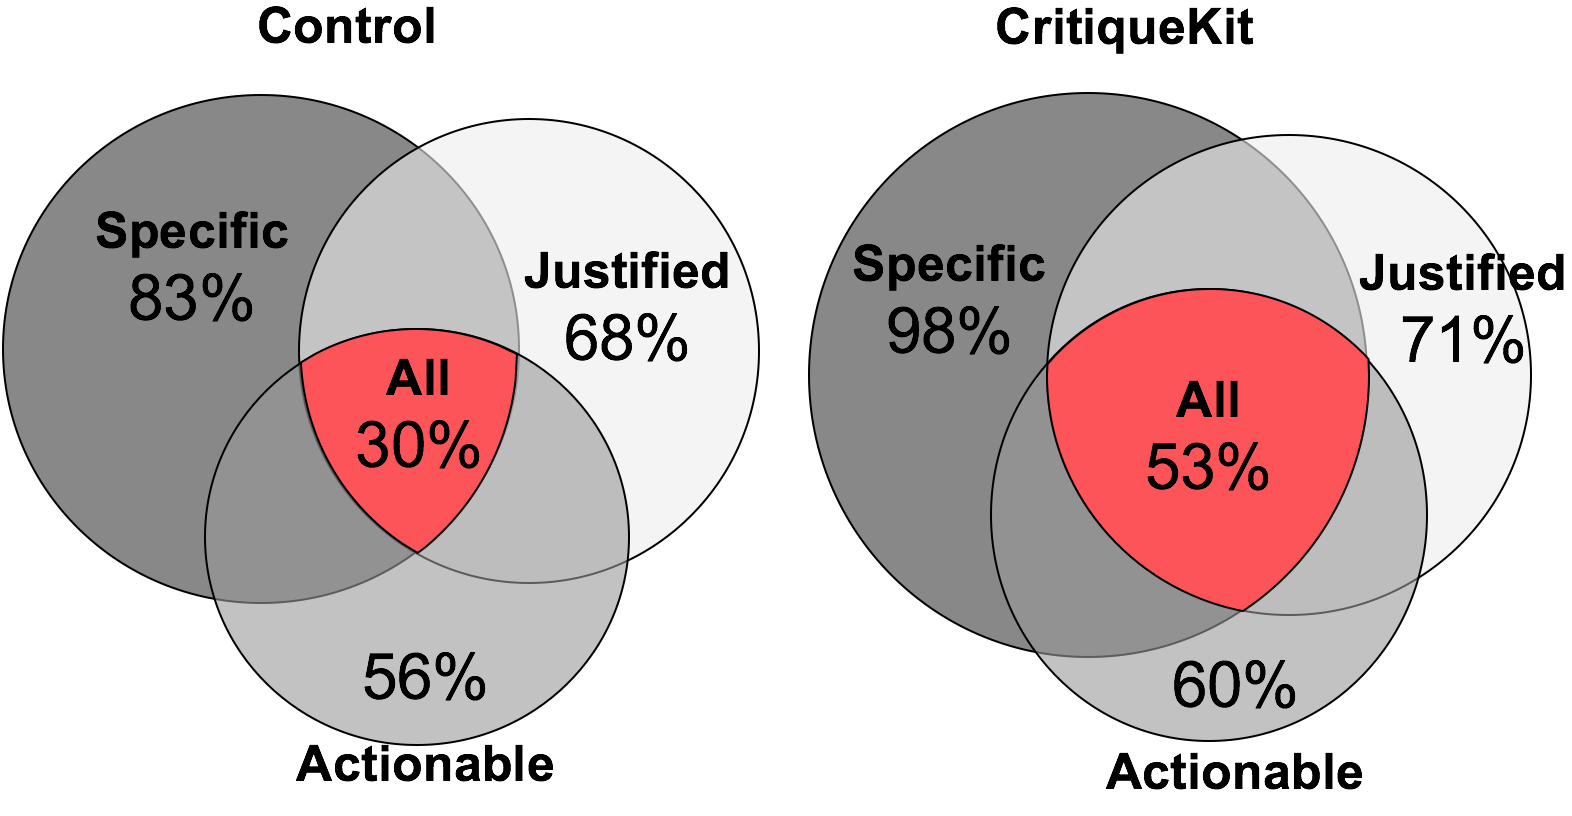
\includegraphics[width=0.6\textwidth]{critiquekit/figures/venn_diagram_exp2.png}
  \caption{In EXP 2, a significantly higher percentage of feedback in the CritiqueKit condition (53\% versus 30\%) contained three attributes of good feedback: Specific, Actionable, and Justified.}~\label{fig:critiquekit_exp2}
\end{figure}

\begin{figure}[b!]
\centering
  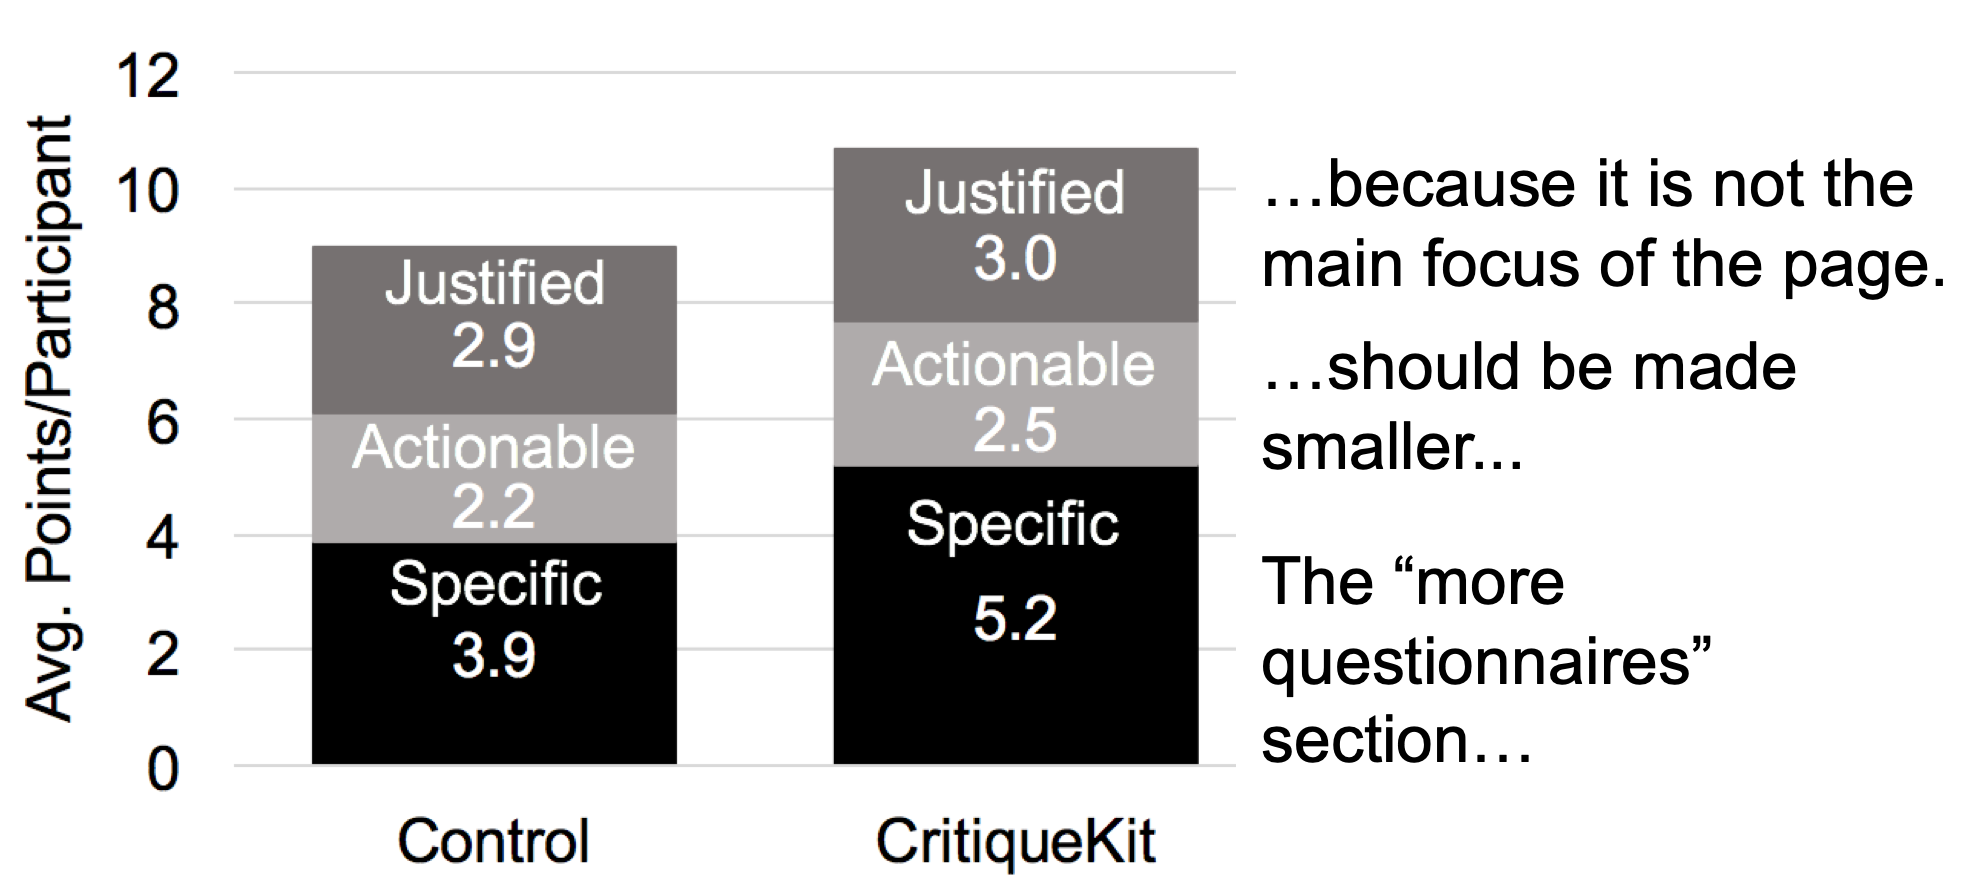
\includegraphics[width=0.6\textwidth]{critiquekit/figures/exp2_bar.png}
  \caption{CritiqueKit participants provided more \textit{specific} and \textit{all-three} category ideas than control participants.}~\label{fig:critiquekit_exp2_bar}
\end{figure}

Because longer comments were more likely to contain all three categories, each comment was also scored on a point scale and averaged per participant. Comments received one point for each specific, actionable, and justified idea (\autoref{fig:critiquekit_exp2_bar}). A \textsc{manova} with category points as dependent variables shows a significant difference between conditions ($F(1,3) = 3.21, p < .005$). CritiqueKit participants provided more specific ideas than Control participants (Control $m = 3.87$, CritiqueKit $m = 5.17$, $F(1,156) = 14.04, p  <  .05$). This may be because the suggestions provided examples of relevant ideas and led CritiqueKit participants to address more. CritiqueKit participants also provided more ideas that fit all three categories than control (Control $m = 1.0$, CritiqueKit $m = 2.2$, $F(1,156) = 8.78, p < .005$). Given that most participants did not have any design experience, the combination of adaptive suggestions and guidance may have been most useful for these reviewers. The suggestions may have provided a starting point while the guidance panel helped them understand how to apply the attributes of good feedback. There were no significant differences in the average number of actionable and justified ideas in comments.

On average, Control comments were 39.3 ($SD = 30.3$) words long and 43.7 ($SD = 31.4$) words for CritiqueKit comments. There was no significant difference in comment length ($F(1,156) = 1.77, p = .19$). Unfortunately, we don't know how the feedback improved students' work because they received feedback from both Control and CritiqueKit participants. A longitudinal deployment with the final version of CritiqueKit would likely be more useful in determining the helpfulness of feedback.

\subsubsection{Suggestions Helped Reviewers Describe Their Thoughts}
Participants rated the suggestions as being generally helpful ($m = 4.29, SD = 0.95$, 1-5 Likert Scale). When asked to elaborate on their rating, many participants noted that the suggestions helped them describe their thoughts. One participant remarked, ``\textit{I was a bit lost at first because I didn't know how to describe my thoughts. The suggestions helped me figure out how I should describe what I was thinking}.'' Similarly, another mentioned that ``\textit{when I [didn't] know how to put my feedback in words, I could look at the suggestions}.'' Particularly for participants without any design experience, suggestions helped with appropriate language to use in their feedback. For example, one noted that ``\textit{seeing actual wording from a designer's point of view was good so you know how to say what you want to say}.'' Though a few participants did not directly select suggestions, it is likely that they were inspired or influenced by them as they used similar wording in their own comments. 

Still, some participants felt the suggestions were too general and not entirely relevant to the specific design they were reviewing. One participant felt constrained by the suggestions, stating that she ignored them because she wanted to write her own opinions. Suggestions seemed most helpful for participants who used them as a starting point for their own thoughts rather than solely relying on them. Participants who simply selected suggestions tended to list issues without adding their own elaboration. This behavior not only led to incomplete feedback, but also produced depersonalized and scattered comments. For example, one comment that solely relied on suggestions reads ``User immediately knows the purpose of the prototype. Good use of grid layout to keep items aligned. Icons should be immediately recognizable to the user.'' A consideration for future work is to develop feedback suggestions tailored to help reviewers provide more cohesive and contextual comments. 

Most participants in this experiment did not have any design experience and may have benefited most from the suggestions. Many participants noted using the suggestions as a way to find ideas whereas students with design experience may already have heuristics and processes in mind when providing feedback. Future work should examine how suggestions and guidance might improve feedback for more experienced learners as well.

\subsubsection{Interactive Guidance Helped Remind \& Focus Reviewers} 
Participants were mixed on the helpfulness of the guidance panel ($m = 3.67, SD = 1.2$, 1-5 Likert Scale). Those who did find it helpful noted that the categories helped guide their feedback process. For instance, one participant noted that he ``\textit{went in order of the checkboxes. First, I provided something specific, then something actionable, then justified it}.'' Another noted that the categories helped her know whether her feedback was actually useful or helpful, and one noted that the guidance panel ``\textit{[made] sure the feedback is complete and not vague}.'' 

Anecdotally, we observed that when participants said the categories were not useful, it was because they believed them to be inaccurate in their classifications. The accuracy (compared to human raters) for the actionable category was 67\% and 75\% for the justified category. A participant stated that ``\textit{[the checkboxes] didn't always check when I thought they should, so I would just do it myself}.'' Another thought the checkboxes were ``\textit{quick to judge, it felt like it wasn't reading what I was saying}.'' Three participants, who were not native English speakers, found the categories confusing because they weren't sure what they meant. Future iterations of CritiqueKit could include the definition of these categories in the prompts to make the meaning clearer. Interestingly, a couple participants noted that they used the categories as reminders rather than for active guidance. For instance, a participant mentioned that though he felt the interactive guidance was not that accurate, ``\textit{[the checkboxes] reminded me to make sure my comment contained specific, actionable, and justified parts, so I'd go and reread through my comment}.'' 

Some participants commented on the adaptive presentation of the suggestions with the guidance panel. For one participant, the suggestions helped him understand what the categories meant. He noted, ``\textit{The whole actionable and justified thing, I didn't know what that meant, so the suggestions helped with that}.'' Observations of participants showed that some clicked on the checkboxes simply to see the suggestions under each one. When asked about how useful they found CritiqueKit in general, participants varied widely in their ratings of usefulness. A more precise measure would allow participants to compare across conditions, which was not possible with this between-subjects design. 

\section{General Discussion}
This chapter empirically investigated two techniques for scaffolding feedback: reusable feedback suggestions and adaptive guidance. This work complements this dissertation more broadly, highlighting the benefits of adaptive guidance for interfaces that support creative tasks. Here we discuss and synthesize the findings.  

\subsection{Generating Reusable Feedback Suggestions}
This work investigated whether suggestions and guidance can scaffold the feedback process. For this strategy to work, an eye towards reuse and adaptive feedback must be adopted. As Schön argues, experts may be most capable of recognizing common patterns and giving useful feedback \cite{Schon1983}. However, while feedback should be specific, underlying concepts can generalize across contexts. In the studies that used expert-generated feedback suggestions (DEP 1 and EXP 2), participants cited the same reason for why the suggestions were useful: as inspiration. Participants reported that the suggestions helped them find words for their thoughts or helped direct their attention to issues they did not originally notice. This suggests that reusable suggestions should focus attention to common issues rather than specific instances. Our approach demonstrates how expertise on creative work can be scaled by providing feedback on a few to apply to many \cite{Kulkarni2013}. This extends work on reusable feedback in coding and writing \cite{Brooks2014, Hartmann2010, Head2017} while keeping the human in the loop, enabling novices to learn and reuse expert insights. 

It is possible that more general suggestions can lead to less personalized feedback, particularly in abstract domains like visual design. We observed this in 7 of the 79 comments from the CritiqueKit condition in EXP 2, in which the four participants simply selected suggestions without further elaboration. A consideration for creating and presenting reusable suggestions is how these suggestions can be both general yet personal to be more helpful to the recipient. 

\subsection{What is the Best Way to Guide Feedback?}
Prior empirical work on feedback (\textit{e.g.}, Kulkarni \textit{et al.} \cite{Kulkarni2013} and Krause \textit{et al.} \cite{Krause2017}) has not compared static and adaptive suggestions. In this chapter, we found that people rarely used static suggestions and did not find them helpful; adaptive suggestions were used more and found more helpful. This reinforces prior work demonstrating that adaptive presentation of examples can improve learning \cite{Lee2010, Najar2014}. By presenting feedback suggestions that directly addressed missing characteristics of a reviewer's feedback, reviewers were prompted on where they could specifically improve, and explicitly shown examples of how to do so. 

The second experiment adapted feedback suggestions based on whether their feedback was categorized as specific, actionable, and/or justified. Though some of the prototype's categorizations were misleading or inaccurate (for example, the comment ``user flow is simple'' was categorized as ``Is Actionable'' because of the word ``use'', even though it lacks a concrete suggestion), participants still referenced the three categories when composing their comments. The guidance panel was useful as a reminder to include the attributes of good feedback in their comments. A more sophisticated method for categorization would likely be helpful, though our naïve approach performed reasonably well overall.

The guidance panel focused on three important attributes of good feedback. A consideration is to also provide guidance for emotional content in feedback, as emotional regulation is important to how learners perceive feedback \cite{Krause2017, Varlander2008}. In addition, other characteristics may also contribute to perceived helpfulness, such as complexity or novelty \cite{Krause2017}, that could be further explored through adaptive guidance.

\subsection{Creating Adaptive Feedback Interfaces}
In order for adaptive guidance to be most effective, the interface should be suitable for adaptation. In the two deployments and first experiment, the suggestions were not curated in any way: more than 1,400 comments were supplied as suggestions, but only 76 of these were reused by reviewers. Having more suggestions available was not beneficial because the suggestions were not sufficiently adaptable and were potentially irrelevant and difficult to browse. EXP 2 introduced a curated approach: experts provided the suggestions with generalizability in mind. Of the 47 suggestions created, 29 were reused. Though fewer suggestions were available, they were more general and adaptable, potentially making them more useful. 

Suggestion presentation shares many properties with search interfaces. Like with search, a good result needs to not only be in the set, but toward the top of the set \cite{Hearst2009Book}. The second experiment contained fewer suggestions, enabling easier search and browsing. Effective curation and display of suggestions should take into consideration the quality of feedback suggestions and how likely they are to be selected, potentially using frequency or some measure of generalizability as a signal. 

\section{Conclusion}
Looking across the deployments and experiments, adaptive suggestions and interactive guidance significantly improved feedback while static suggestions did not offer significant improvements. These techniques were embodied in the CritiqueKit system, used by 95 feedback providers and 336 recipients. Future work should examine applying other attributes of helpful feedback and further investigate how best to create, curate, and display adaptive suggestions. 

Much knowledge work features both underlying principles and context-specific knowledge of when and how to apply these principles. Potentially applicable feedback and review areas include domains as disparate as hiring and employee reviews, code reviews, product reviews, and reviews of academic papers, screenplays, business plans, and any other domain that blends context-specific creative choices with common genre structures. We hope that creativity support tools of all stripes will find value in the ideas and results presented here.


\section{Acknowledgements}
We thank Kandarp Khandwala and Janet Johnson for help rating feedback. This research was supported in part by a fellowship from Adobe Research.

This chapter, in part, includes portions of material as it appears in \textit{Interactive Guidance Techniques for Improving Creative Feedback} by Tricia J. Ngoon, C. Ailie Fraser, Ariel S. Weingarten, Mira Dontcheva, and Scott Klemmer in the Proceedings of the 2018 CHI Conference on Human Factors in Computing Systems (CHI '18). The dissertation author was one of the primary investigators and authors of this paper.


% % Load basic packages
% \usepackage{balance}       % to better equalize the last page
% \usepackage{graphics}      % for EPS, load graphicx instead 
% \usepackage[T1]{fontenc}   % for umlauts and other diaeresis
% \usepackage{txfonts}
% \usepackage{mathptmx}
% \usepackage[pdflang={en-US},pdftex]{hyperref}
% \usepackage{color}
% \usepackage{booktabs}
% \usepackage{textcomp}
% \usepackage[sort,nocompress]{cite}
% \usepackage{perpage}
% \MakePerPage{footnote}
% \usepackage{multirow}
% \usepackage[bottom,flushmargin,hang,multiple]{footmisc}
% \usepackage{dblfloatfix}    % To enable figures at the bottom of page

% % Some optional stuff you might like/need.
% \usepackage{microtype}        % Improved Tracking and Kerning
% % \usepackage[all]{hypcap}    % Fixes bug in hyperref caption linking
% \usepackage{ccicons}          % Cite your images correctly!
% % \usepackage[utf8]{inputenc} % for a UTF8 editor only

% If you want to use todo notes, marginpars etc. during creation of
% your draft document, you have to enable the "chi_draft" option for
% the document class. To do this, change the very first line to:
% "\documentclass[chi_draft]{sigchi}". You can then place todo notes
% by using the "\todo{...}"  command. Make sure to disable the draft
% option again before submitting your final document.
% \usepackage{todonotes}
\chapter{Sharing the Studio: How Creative Livestreaming can Inspire, Educate, and Engage}

\begin{figure}[b!]
\centering
  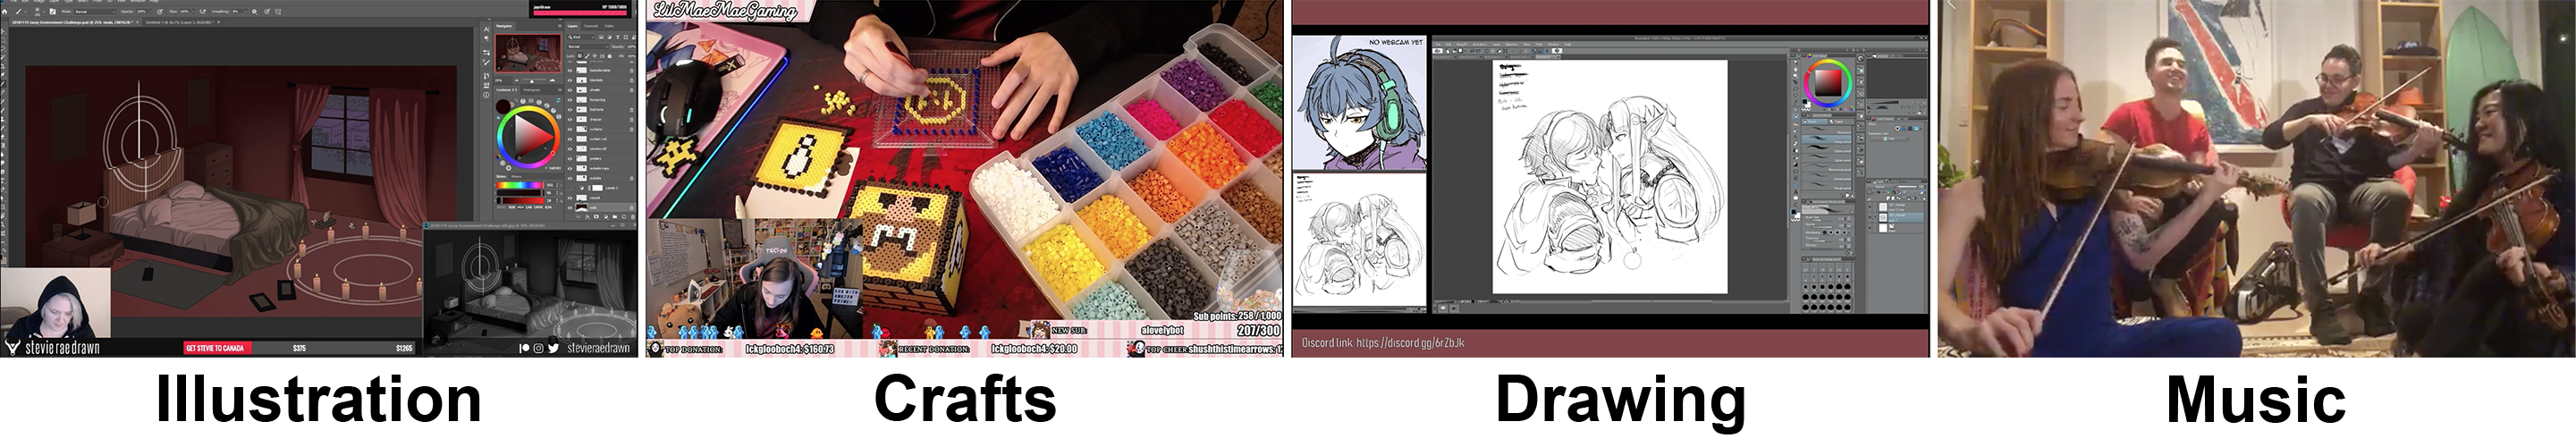
\includegraphics[width=\textwidth]{livestreams/figures/examples-horizontal.png}
  \caption{Examples of creative livestreams on Twitch, YouTube, and Facebook. Artists stream videos of themselves working on creative projects\protect\footnotemark.}~\label{fig:livestream_examples}
\end{figure}


%\vspace{-20pt}
%Artists communicate and share their creative work through online galleries, creative communities, and social media. While some go further and also share works-in-progress or videos of their process, these still present a selective, edited view. Livestreaming, in contrast, allows creators to share an authentic, unedited view of their process while they work. 
Many artists livestream their creative process, allowing viewers to learn and be inspired from the decisions -- and mistakes -- they make along the way. This paper presents the first broad look at the range of creative activities people stream. Through content analysis of livestream archives, interviews with 8 streamers, and online surveys with 165 viewers, we study current practices and challenges in creative livestream communities and compare them with prior observations of livestreaming in other domains. We observed four common types of creative livestreams: teaching, making, socializing, and performing. We identify three open questions for the research community around how to better support the goals of creative streamers and viewers: how to support richer audience interactions at scale, how to support all parts of the creative process, and how to support watching livestream archives.


% % STATE OF THE WORLD
% Many artists working with both digital and physical tools livestream their process as they work on a project.
% % THE BIG BUT
% Despite this, research on livestreaming has primarily focused on gaming, pedagogical, and software engineering use cases. 
% % PROBLEM
% As a result, livestreaming platforms are not always designed with creative work in mind. 
% %<SOME PROBLEM HERE: maybe something about how livestream communities and tools are designed for screensharing, making assumptions like artists will have their hands or eyes free to pay attention to chat, etc.>
% % INSIGHT
% %By understanding creative livestreams, we can broaden our understanding of how to design streaming tools for a large portion of the livestreaming community.
% % APPROACH
% We present a first comprehensive look at creative livestreams, a growing medium where people share a window into their work as it unfolds. 
% % WHAT WE DID
% Through content analysis of livestream archives, online surveys with 165 viewers, and interviews with 8 streamers, we address current challenges in online creative livestream communities and compare them with prior observations of livestreaming in other domains.
% %we build on our understanding of livestreaming practices by focusing on the space of creative livestreams. We address current challenges in these online communities and compare them with prior observations of livestreaming. 
% We find that, unlike other domains, one of the main reasons viewers watch creative livestreams is for inspiration and motivation. One dominant challenge that emerged for streamers was balancing between their work and interacting with viewers. This is especially difficult for creative work, which often requires the artist's full attention. We propose opportunities for future research to better support the needs of viewers and streamers of creative work.
% %Or a lot of artists who livestream are not educators, so they are not used to that kind of multitasking.
% %<CAVEAT UNIQUE TO CREATIVELIVESTREAMING>
 

\section{Introduction} % or something more descriptive

%Browsing and exploring inspiring examples \cite{Shneiderman2007, Shneiderman2002, Greene2002, Herring2009, Bawden1986} and interacting with and getting feedback from other people \cite{} are both key parts of the creative process. Creative communities have existed for a long time to address these needs. Such communities often organize around sharing portfolios or completed projects (\textit{e.g.,} 500px, Behance and Dribbble\footnote{\url{500px.com}, \url{behance.net}, \url{dribbble.com}}). In recent years, creative communities have begun to form around a new medium for sharing not only final work, but the process behind it: livestreaming. 

%authenticity is the hot commodity now
%tech offers a window into a kind of authenticity that used to be harder to get
%\xxx{vignette sooner?}
Artists communicate and share their creative work through online \& on-land galleries, communities, and social media \cite{Kim2017}. Some also share works-in-progress, how-to tutorials, and videos describing the process that leads them to a final product. Prior work has shown that seeing and sharing the creative process is beneficial for creativity \cite{Kim2017}. However, these highly curated windows into process require time and effort for the creators to produce and share. 
%To create a good video tutorial, one has to set up an appropriate project, practice, record, and finally edit out mistakes or irrelevant parts \xxx{<-- xxx says move later but where?}. And works-in-progress communities are harder to find, as artists hesitate to mix works-in-progress with final work in their portfolios \cite{Kim2017}.\xxx{fine to move these two sentences to later. Not sure where. Can comment them out for now.}

\stepcounter{footnote}\footnotetext{Sources for video screenshots, from left to right: \href{http://bit.ly/2SK5zWE}{\nolinkurl{bit.ly/2SK5zWE}}, \href{http://bit.ly/2Bv9Y69}{\nolinkurl{bit.ly/2Bv9Y69}}, \href{http://bit.ly/2SJYFRa}{\nolinkurl{bit.ly/2SJYFRa}}, \href{http://bit.ly/2TK12Rq}{\nolinkurl{bit.ly/2TK12Rq}}}

Many artists have begun to broadcast live video as they work on graphic design, crafting, drawing, or music through platforms like Twitch and YouTube\footnote{\href{www.twitch.tv}{\nolinkurl{twitch.tv}}, \href{www.youtube.com}{\nolinkurl{youtube.com}}}. Livestreaming allows creators to share their unedited process \emph{while} they work. These videos usually feature the artist's workspace, %(\autoref{fig:livestreaming_view}a)
a view of their face,
%(\autoref{fig:livestreaming_view}b)
and their audio narration as they work (\autoref{fig:livestream_examples}). Viewers get an inside look into the creative process, learning from artists' decisions, mistakes, and surprises~\cite{Faas2018, Haimson2017}.  
%artists make along the way. 
Some also interact with artists directly via text chat. 
%Livestreaming shows everything, including mistakes, surprises, and dull moments . 
%Livestreaming has grown as a medium for sharing all kinds of content, from video gaming to travelling.
%Livestreaming has democratized the practice of sharing process, allowing anyone with a camera and internet to share their own process with the world.
%Livestreams provide a unique form of social engagement, allowing both one-to-many interaction of streamers to viewers, and many-to-many interaction among viewers \cite{Hilvert-Bruce2018, Hu2017}. 
Communities have formed around creative livestreaming, including dedicated platforms such as Picarto\footnote{\href{www.picarto.tv}{\nolinkurl{picarto.tv}}}.
Livestreaming democratizes the studio-apprentice model, enabling anyone to see experts' in-context choices by working alongside them \cite{Schon1985}. 
%Now anyone can sit in Leonardo da Vinci's studio and learn from the best. %something about making creative process accessible.

This paper seeks to understand what makes creative livestreaming so appealing for those who stream and those who watch.
%Some of these can include creative livestreams, \textit{e.g.,} programming is often considered creative, and many cultural heritage and knowledge-sharing activities are also creative, such as traditional calligraphy or drawing tutorials. But this still leaves a wide range of creative activities being livestreamed that are not yet understood. 
We provide the first broad look at the range of creative activities people stream. 
%By understanding creative livestreams, we can broaden our understanding of how to design streaming tools for a large and growing portion of the livestreaming community. 
Perhaps the three most popular genres for livestreams are video gaming \cite{Pellicone2017, Lessel2017, Sjoblom2017, Hamilton2014}, programming \cite{Faas2018, Haaranen2017}, and lifestyle  \cite{Lu2018a, Tang2016}. This paper looks at the use of livestreaming to share the process behind creating an original artifact. We use Twitch's definition of creative work: ``visual art, woodworking, costume creation, prop building, music composition, or any other process in which you entertain and connect around a creative activity'' \cite{Moorier2015}. These activities focus on creating a novel artifact, unlike typical video games or lifestyle streaming.

% YO:
%maybe also: previous work focuses more on building communities and performing in order to establish a certain audience. but not all creative streams do that, many just want to share their process
%freelancers are home a lot, many of their viewers are also freelancers or aspiring professionals, livestreams let you stay connected / have a coworking space to stay connnected with others while physically alone
%People go to Live streams to feel less alone at home working on their own thing. Since we know many people work while they are watching/listening to live streaming we can think of it as a virtual co-working space where you are working with your friends?

%The real-time interactivity and live participation that livestreams provide are engaging for viewers because they can be a part of the livestream \cite{Wohn2018}, and have the opportunity to change its outcome \cite{Lu2018a}.

%We find that streamer needs and viewer expectations differ considerably based on the type of creative stream, and creative livestreaming requires considerable preparation and strategic attention management.

We explore three main questions: 
\begin{enumerate}
    \item \textbf{What are creative livestreams?} For a general sketch of creative livestreams, we present a content analysis of a sample of livestreams that illustrates the range of content people stream and the different types of creative livestreams.
    \item \textbf{Why and how do people stream creative work?} Which parts of their process do they stream? To understand streamers' motivations, processes, and challenges, we present findings from interviews with 8 creative livestreamers and compare their experiences with streamers in other domains.
    \item \textbf{Why do people watch creative livestreams?} To understand the audience these streamers reach, we present findings from three online surveys with 165 viewers that highlight learning and inspiration as key motivators, with entertainment and community close behind.
\end{enumerate}

We found that viewers often seek to learn and be inspired from creative livestreams. Notably, inspiration is a much more prominent theme compared with prior work in other livestreaming domains such as gaming. However, many streaming platforms are not designed to support these goals. Audience engagement is particularly important for streamers, but can be difficult to achieve because of the conflicting goals different viewers may have and the deep focus creative work often requires.
% if authenticity is biggest takeaway, highlight it earlier. more problem solving in intro rather than taxonomizing.
% how do we expose authentic energy of people to mobilize the next gen of creatives?
% mistakes, liveness, risk, connection
\begin{figure}[b]
\centering
  \includegraphics[width=1\columnwidth]{livestreams/figures/livestreaming_paper_figure_anonymized.jpg}
  \caption{A typical creative livestream setup. (a) A camera or screencast displays the artist's workspace. (b) A second camera shows the artist's face. (c) Graphical overlays provide ambient information about the artist (\textit{e.g.,} social media pages) and display interactions with the audience (\textit{e.g.,} pop-ups that appear when viewers subscribe or donate to the stream). (d) Live chat allows viewers to communicate with the streamer. }~\label{fig:livestreaming_view}
  \vspace{-0.15in}
\end{figure}

\section{What are creative livestreams?}
Popular livestreaming platforms include Twitch, YouTube, Facebook, Instagram, and Periscope. Picarto, a livestreaming platform dedicated to creative work, launched in 2013. Twitch launched its \textit{Creative} category in 2015 \cite{Moorier2015}. To deal with its explosion in popularity, Twitch replaced the \textit{Creative} category with six more-specific categories in September 2018: \textit{Art}, \textit{Music \& Performing Arts}, \textit{Science \& Technology}, \textit{Beauty \& Body Art}, \textit{Food \& Drink}, and \textit{Makers \& Crafting} \cite{Robertson2018}. 
%\xxx{Also, would it be interesting to note the \# of streamers or avg \# of streams in that category?}\xxx{can't get those numbers via the twitch api. figure 2 is the best i could do} 
%\xxx{I agree with xxx. Why is Twitch the one platform you call out here?} \xxx{i mention youtube and picarto below (moved picarto up sooner), is there something more i should say? can't isolate creative streams with certainty on youtube. can't find a usable \textsc{api} for periscope. } 
Creative livestreams also appear on many other platforms, but often without a distinct category. For example, many creative streams on YouTube are categorized as \textit{Education}, \textit{How-to \& Style}, or even \textit{Gaming}.

Livestream videos (\autoref{fig:livestreaming_view}) typically show the artist's full screen (when working on a computer) or workspace (for physical work) and a camera view of their face. Livestreams usually also feature a live chat, allowing viewers to communicate with each other and the artist. 

To learn more about creative livestreams, we studied two popular platforms: Twitch and YouTube. As these large platforms cover many types of content, we narrowed our investigation to the \textit{Creative} category on Twitch and the \textit{Adobe Live} video series on YouTube. Through this, we see how streams and communities differ across platforms.  
%For example, on Twitch anyone is welcome to stream, while Adobe invites special guest artists to their studio. On Twitch its up to each artist to make their stream engaging, while Adobe invites hosts to help engage with the audience. 
%This section provides an overview of two popular creative livestreaming communities: the Creative category on Twitch, and livestreams hosted by Adobe. We focus on these communities as they are hosted through popular platforms (Twitch and YouTube), which are the two most frequently-mentioned platforms by survey respondents who watch creative livestreams.

\subsection{Creative livestreams on Twitch: Content analysis}
To better understand the format and content of creative live\-streams, we analyzed a sample of videos on Twitch, one of the most popular platforms for livestreaming. For each creative category, we gathered aggregate metrics about streamers and viewers. We watched and took notes on a sample of 29 videos. We identified four common types of creative livestreams that will appear throughout the paper: \textit{Teaching}, \textit{Making}, \textit{Socializing}, and \textit{Performing}.

\subsubsection{Methodology}
To measure the popularity and activity in each of the six creative categories, we queried the Twitch \textsc{api} 4 times a day for 7 days to obtain the number of currently-live streams and number of currently-watching viewers in each category.

We also used the Twitch \textsc{api} to download metadata about the videos in each category (limited to top 600)
%Because this \textsc{api} halts video requests after 600 videos, so our script downloaded metadata for the 600 most-viewed videos in each category. The script 
and randomly selected 50 archived English livestream videos. Four annotators (including the first author) watched each of these videos. Ten videos were not available for viewing and thus excluded (either because their archive expired between being downloaded and being annotated, or because they were only available to subscribers of a channel). Another 11 videos were excluded as they showed video games, TV show reruns, or live event coverage. While these videos were categorized as creative on Twitch, they did not reflect our definition of creative work, namely the creation of a novel artifact. This yielded 29 videos. For each, annotators took notes in a structured spreadsheet on the content presented, camera setup, overall structure of the stream, artist's presentation style, and chat activity.

\begin{table}[b]
\centering
\caption{Summary of popularity of Twitch's creative livestream categories. The number of currently-live streams and currently-watching viewers were collected 4 times a day for a week and then averaged.}~\label{table:livestream_summary}
\begin{tabular}{llll}
\textbf{Category}        & \textbf{\begin{tabular}[c]{@{}l@{}}Avg. \#\\ livestreams\end{tabular}} & \textbf{\begin{tabular}[c]{@{}l@{}}Avg. \# live\\ viewers\end{tabular}} & \textbf{\begin{tabular}[c]{@{}l@{}}Avg. \# viewers\\ / stream\end{tabular}} \\
Art                      & 339                                                                    & 6417                                                                    & 21                                                                          \\
Beauty \& Body Art       & 5                                                                      & 177                                                                     & 17                                                                          \\
Food \& Drink            & 19                                                                     & 1088                                                                    & 64                                                                          \\
Makers \& Crafting       & 40                                                                     & 680                                                                     & 16                                                                          \\
Music \& Performing Arts & 286                                                                    & 6881                                                                    & 24                                                                          \\
Science \& Technology    & 91                                                                     & 1155                                                                    & 12                                                                         
\end{tabular}
\end{table}

While this sample does not capture all types of creative activities one might livestream, our hope is that by analyzing a set of canonically creative activities we can shed light on a broader set of activities that might also have a creative component (\textit{e.g., } video games that involve creating artifacts).
%There is overlap among categories on Twitch, even sometimes within a single livestream when an artist switches back and forth between creative work and other activities like gaming. 

\subsubsection{Results: Most streamers focus on work \& engage with viewers}
\autoref{table:livestream_summary} shows overall metrics for the creative categories on Twitch. The most popular categories by far are \textit{Art} and \textit{Music \& Performing Arts}. The category with the most viewers watching per stream is \textit{Food \& Drink}, likely because there are fewer streams to choose from relative to the number of interested viewers. These communities are small relative to the most popular games; for example, the game Fortnite has between 5,000 and 10,000 streams live on Twitch at any given time, with around 100,000 total viewers watching. %\xxx{xxx says move earlier but where?}

\begin{table}[b!]
\centering
\caption{Creative activities shown in a random sample of 29 livestreams from Twitch's creative categories, and the primary type of structure each stream exhibits.}~\label{table:livestream_activities}
\begin{tabular}{lll}
\textbf{Category}        & \textbf{Activity (\# videos if \textgreater 1)} & \textbf{\begin{tabular}[t]{@{}l@{}}Primary type\\ of stream\end{tabular}} \\
Art                      & Multimedia production                           & Making                                                                    \\
                         & Digital drawing (4)                             & Making                                                                    \\
                         & Animation                                       & Teaching                                                                  \\
                         &                                                 &                                                                           \\
Beauty \& Body Art       & Makeup                                          & Socializing                                                               \\
                         & Makeup (3)                                      & Making                                                                    \\
                         &                                                 &                                                                           \\
Food \& Drink            & Cooking                                         & Teaching                                                                  \\
                         &                                                 &                                                                           \\
Makers \& Crafting       & Making foam props                               & Teaching                                                                  \\
                         & Sewing quilts                                   & Socializing                                                               \\
                         & Bead art (2)                                    & Making                                                                    \\
                         & Assembling models                               & Making                                                                    \\
                         & Assembling models                               & Socializing                                                               \\
                         & Woodworking                                     & Making                                                                    \\
                         & Pottery                                         & Making                                                                    \\
                         &                                                 &                                                                           \\
Music \& Performing Arts & Music production                                & Performing                                                                \\
                         & Music production                                & Making                                                                    \\
                         & Acting \& improv games                          & Performing                                                                \\
                         &                                                 &                                                                           \\
Science \& Technology    & Building a computer                             & Making                                                                    \\
                         & Programming (3)                                 & Making                                                                    \\
                         & Game development (2)                            & Teaching                                                                  \\
                         & Talking about technology                        & Socializing                                                              
\end{tabular}
\end{table}

The videos span a range of creative activities (\autoref{table:livestream_activities}). The average video length was 3h46m, not including time spent gaming -- a few artists combined both creative work and video gaming into one stream, spending the first part on creative work then switching to gaming when they were finished. The shortest video was 1h3m; the longest was 7h56m. These videos are notably longer than most non-livestream videos.

Almost all videos contained either a screencast view for work being done on a computer (13/29) or a camera view for physical work (15/29). One showed a distant camera view of the artist producing music in a studio. Most (26/29) showed the artist's face: in 10 as part of the main camera feed, and 16 as a separate feed overlaid in a corner (as in \autoref{fig:livestreaming_view}). Almost all artists (27/29) talked out loud while streaming; of the two silent streamers, one occasionally posted in the chat. Most artists talked about a mix of their work and other topics (18/29). Some talked only about their work (9), or only about other topics (1). One was a variety show, so the talking \textit{was} the work. Many videos (19/29) included background music. 

Most artists engaged with the chat at least sometimes (24/29). 18 artists engaged frequently with the chat, and 6 occasionally. Three videos did not show a chat replay despite the artist referring to the chat; we assume it was not saved or had been hidden. In all 26 remaining videos, viewers asked questions at least occasionally, or in some videos (9/26) frequently. In half of these videos, all chat questions appeared to get answered; in the rest, some (7/13) or many (4/13) questions went unanswered. In 2 videos, most chat questions were answered by other viewers or moderators in the chat.

\subsubsection{Four common types of creative livestreams}
We identified four common types of creative livestreams. We also observed these in interviews with streamers in the next section. Sj{\"{o}}blom \textit{et al.} \cite{Sjoblom2017a} offer a similar characterization of video game livestreams; we found some key differences and fewer overall types of structures. \autoref{table:livestream_activities} shows the primary type of each stream in our sample set. These are general high-level trends; some streams bridge multiple types.

\textbf{Teaching} streams have an instructional focus, where the stream\-er is educating the viewers. These include step-by-step how-to demonstrations of tasks such as cooking a recipe, producing a photo-editing effect, or creating DIY costumes. Other examples include critiquing others' work, answering viewers' questions, or explaining a topic.

\textbf{Making} streams focus primarily on creative work and process, but not explicit teaching. These include an artist silently drawing, a streamer attempting a new task they have not tried before and talking their way through it, and an artist making pottery and describing \textit{what} they are doing but not \textit{how}. 

\textbf{Socializing} streams feature the streamer chatting casually with viewers, often while working on a project, such as makeup or sewing (but the project is not the main focus). These are often described as ``chill'' streams. Socializing streams often have tight-knit communities; the streamer will recognize the names of viewers in the chat and ask them how they are doing.

\textbf{Performing} streams feature the artist performing their work. Naturally, these mostly include performative arts like music and acting (\textit{e.g.,} as opposed to drawing). Like with Making, the focus is on the artist's work; in this case the artist does not talk about what they are doing, they just do it. Performing streams differ from non-live recordings in that they often take a more casual improvisational form, rather than scripted performance (\textit{e.g.,} musical ``jam sessions'' or improv acting).

Within each type, the amount of interaction between the stream\-er and the audience varies. Some streamers hold ``request streams'' or ``Q\&A streams'', where the content and flow are determined by audience requests or questions, respectively. Some hold contests or games. A request stream could have audience members requesting songs for a Performing stream, a topic for a Teaching stream, or a particular artifact for the artist to make in a Making or Socializing stream. 

\subsection{Creative livestreams go professional}
While many livestreams are run by individuals, professionally-run livestreams are also growing in popularity. Adobe, a company that produces creative software, hosts livestreams on a regular schedule multiple times a week\footnote{\href{https://behance.net/live}{\nolinkurl{behance.net/live}}}. These can be viewed on Behance or on Adobe's Creative Cloud YouTube channel. They host two livestream series: \textit{Adobe Live} is a Making stream that happens for 6 hours (three 2-hour sessions) three days a week, and it features guest artists usually hosted by someone who works at Adobe. \textit{Daily Creative Challenges} is a Teaching stream that happens for 30 minutes five days a week. It complements contests organized by Adobe to teach new skills. YouTube reports these streams having between 2,000 and 8,000 views each; it does not distinguish between live and replayed views.

\stepcounter{footnote}
\begin{figure}[b]
\vspace{-0.1in}
\centering
  \includegraphics[width=1\columnwidth]{livestreams/figures/adobelive.png}
  \caption{The \textit{Adobe Live} series features a guest artist (bottom left) and a host (bottom right). The artist is working on a digital drawing, and the host is looking up at the live chat feed, engaging with the audience (\href{https://youtu.be/yYDmQhg_1uE}{\nolinkurl{youtu.be/yYDmQhg_1uE}}). }~\label{fig:livestream_adobelive}
  \vspace{-0.2in}
\end{figure}

\textit{Adobe Live} differs from most streams by featuring two people. Typically there is a host and an guest artist (\autoref{fig:livestream_adobelive}), but sometimes two artists work together. Adobe hosts different artists every week across a range of creative disciplines (\textit{e.g.,} graphic design, UX design, photography, video editing). Typically, the host moderates the stream, responding to chat messages and passing on questions from viewers to the artist so that the artist can focus on their work. When the stream includes two artists, they trade off hosting.
%xxx: removing for now because we haven't talked about challenges for streamers yet
%These livestreams address some of the challenges self-streamers often face, such as facilitating the chat while working and dealing with technical setup, by having separate people take on those tasks. 
The featured artists are usually practitioners, not teachers; their work mainly serves as inspirational demonstrations, while also giving the the community a chance to engage with questions and comments. 

The \textit{Daily Creative Challenges} series features one person who both reads chat messages and provides a short tutorial on a software technique. These livestreams are part of Adobe's Creative Challenges, which are contests that encourage people to use Adobe software and submit design work for prizes\footnotemark. These streams are 30 minutes long -- this is short for a livestream -- and focus on instruction: explaining the challenge of the day and teaching viewers the skill of the day. 

\footnotetext{\href{https://www.behance.net/dailycreativechallenge}{\nolinkurl{behance.net/dailycreativechallenge}}}

%The interviews and surveys in this paper are with a mix of people from Adobe's livestreams and from other creative communities, allowing us to gain a broad understanding of the challenges creative streamers face and suggest possible improvements for them.
\section{Why \& how do people stream creative work?}
%Now that we have a broad understanding of two popular creative livestreaming communities, we seek to go deeper into the motivations and processes behind creative livestreamers. 
What motivates people to livestream creative work? What challenges do they encounter in the process, and how do these compare with streamers in other domains? We interviewed 8 creative livestreamers and found that streamers were primarily motivated by sharing and engaging with their audience. However, they find it difficult to connect with their audience while focusing on their work. Additionally, for many, livestreaming requires significant effort and behind-the-scenes preparation. 

%Streamer motivations and processes seem to be highly dependent on the type of stream they create. Prior work has shown that the main reasons gaming streamers stream are to build a community of like-minded individuals \cite{Hamilton2014, Pellicone2017} and to make money or promote their personal brand \cite{Pellicone2017}. People who livestream about their lifestyle or to entertain do it primarily for personal branding \cite{Tang2016}. In contrast, educational or culture-sharing streamers' main goal is usually to share their knowledge and culture with others \cite{Lu2018a, Lu2019}. As for process, some livestreams are highly produced and require significant preparation beforehand (\textit{e.g.,} e-sports tournaments), while others occur on-the-spot whenever the streamer decides to go live (\textit{e.g.,} many lifestyle streams on Instagram).
%Such streamers often care more about making a broad positive impact and raising awareness about their particular activity than making money or receiving gifts from viewers, even when they do also make money as a side benefit \cite{Lu2019}. 
%We echo Lu et al.'s \cite{Lu2019} finding (maybe) that for many types of creative activities that are usually solitary (e.g., playing a solo musical instrument or doing visual art), streaming allows people to have company while they work so the activity is not so lonely.

\begin{table*}[b]
\centering
\caption{Self-reported background information about the eight creative livestreamers we interviewed. ``Skill'' refers to the streamer's skill at the type of creative work they stream. After interviewing the streamers, we determined the structure type of their most frequent streaming style.}~\label{table:livestream_streamers}
\resizebox{1\textwidth}{!}{
\begin{tabular}{llllllll}
            & \textbf{Role}                                                                       & \textbf{Content}       & \textbf{Skill} & \textbf{Frequency} & \textbf{Platform}                                                              & \textbf{Primary type} & \textbf{Moderators} \\
\textit{P1} & Freelance Digital Illustrator                                                       & Digital Illustration   & Expert         & 3 times / week     & Twitch                                                                         & Making                & Yes        \\
\textit{P2} & \begin{tabular}[t]{@{}l@{}}Video Editor \& Educational\\ Content Maker\end{tabular} & Q\&A, Analyzing Videos & Expert         & Occasional         & YouTube, Instagram                                                             & Teaching              & Yes        \\
\textit{P3} & Artist / Musician                                                                   & Music Improvisation    & Expert         & Occasional         & Facebook, Instagram                                                            & Performing            & No         \\
\textit{P4} & Drawing Hobbyist                                                                    & Digital Drawing        & Intermediate   & Monthly            & Twitch                                                                         & Making                & No         \\
\textit{P5} & Drawing Hobbyist                                                                    & Digital Drawing        & Intermediate   & Monthly            & Twitch, previously Picarto                                                     & Making                & No         \\
\textit{P6} & Adobe XD Evangelist                                                                 & UX Design              & Expert         & Daily - Weekly     & \begin{tabular}[t]{@{}l@{}}YouTube, Facebook,\\ previously Twitch\end{tabular} & Teaching/Making       & Yes        \\
\textit{P7} & Adobe XD Evangelist                                                                 & UX \& Graphic Design   & Expert         & 3 times / week     & \begin{tabular}[t]{@{}l@{}}YouTube, Periscope,\\ Facebook\end{tabular}         & Teaching/Making       & Yes        \\
\textit{P8} & Adobe Designer                                                                      & UX \& Graphic Design   & Expert         & Daily - Weekly     & YouTube, previously Twitch                                                     & Teaching/Making       & Yes       
\end{tabular}
}
\end{table*}



\subsection{Interview methodology}
We recruited 8 streamers (4 male, 4 female, ages 20-45) from personal and professional connections for one-hour semi-structured interviews. We interviewed people across creative disciplines and experience with streaming (\autoref{table:livestream_streamers}). We asked participants about their current position and background, process and motivation for streaming, challenges and successes they have experienced, and strategies for engaging with their audience. Three of the participants also host for \textit{Adobe Live}; we asked them about their experience hosting as well as streaming. We took notes and recorded every interview, and analyzed them by comparing participants' answers and identifying common patterns. Interviews were conducted over video chat (4), audio chat (2), or in person (2). Each participant received a \$15 gift card for their time. 


\subsection{About the streamers}

\textit{P1} is a freelance artist who began streaming her work full-time on Twitch in 2016. For the first two years, she streamed for 20-25 hours a week and spent the rest of her time on stream-related preparation. At this commitment level, streaming was her primary source of income. Income on platforms like Twitch mainly derives from ad revenue, viewer subscriptions, and donations. Over time, this became exhausting and felt unsustainable. \textit{P1} took a break, and now streams casually 3 times a week but not as a primary source of income. Her livestream setup includes a camera view of her face, a screencast of her work, a Stream Deck (\autoref{fig:livestream_streamdeck}), and two monitors for her to see chat activity and other information.

\begin{figure}[b]
\centering
  \includegraphics[width=0.6\columnwidth]{livestreams/figures/streamdeck.png}
  \caption{The Stream Deck is a programmable control pad used by many streamers, including \textit{P1}, for easy access to common shortcuts and actions. It integrates with Open Broadcaster Software (OBS), a program used by many streamers to host their livestreams (\href{https://www.elgato.com/en/gaming/stream-deck}{\nolinkurl{elgato.com/en/gaming/stream-deck}}).}~\label{fig:livestream_streamdeck}
  \vspace{-0.2in}
\end{figure}

\textit{P2} is a video editor and creator who has been making video tutorials on photo and video editing for about 7 years. He hosts a podcast where he interviews people about their creative approach and life stories. He has tried Periscope, and began streaming on YouTube when it enabled mobile streaming in 2017: casual streaming was on the rise. Occasionally he livestreams on YouTube or Instagram, answering viewer questions, teaching a particular topic, analyzing a popular video, or critiquing viewers' work. His setup comprises a camera view of his face, a screencast of his work, and a large monitor for him to see chat activity and other information.

\textit{P3} is a musician who livestreams on Facebook and Instagram (with three band members). Her streams are spontaneous and improvisational; the quartet does not play together regularly but they have a fan base that they stream to whenever they are together. These livestreams require little setup; they are broadcast from a single mobile phone either held by a friend or propped up. She also occasionally livestreams product reviews and behind-the-scenes views of her shows.

\textit{P4} and \textit{P5} are hobby artists who stream digital drawing about once a month on Twitch. They both started livestreaming 2 or 3 years ago. \textit{P5} used to stream on Picarto, and moved to Twitch about a month ago because it was easier to use and tends to attract more viewers as a better-known platform. \textit{P5} rarely talks out loud during her streams (only when nobody else is home) and \textit{P4} never does. Instead, they engage with viewers by typing in the chat. Neither shows their face when streaming; their setups include only a screencast of their drawing window. 

\textit{P6}, \textit{P7}, and \textit{P8} stream as part of their jobs at Adobe by hosting artists, streaming their own work, and teaching Adobe products.
%are all employees of Adobe who regularly stream on Adobe's Daily Creative Challenges, and also host on Adobe Live. 
%These participants stream frequently as part of their jobs, and are all highly experienced at the creative work they stream. 
\textit{P6} has been making video tutorials on photo editing for over 10 years. He briefly tried streaming on Twitch but found that his audience did not transfer over to the new platform. He has been streaming with Adobe for approximately 6 months. \textit{P7} taught courses and training programs on design and illustration software for many years. He has been working at Adobe for 9 years, and streaming with Adobe for about 4 years. 
%\textit{P7} was one of the first evangelists involved in Adobe's livestreaming efforts, which started on Twitch.
\textit{P8} is a designer and trained illustrator and has been streaming with Adobe for 4 years. Before joining Adobe, she used to occasionally stream her art process on Twitch. By virtue of livestreaming professionally, all three participants have fairly sophisticated technology setups, including a camera view of their face in front of a green screen, a screencast of their computer, several displays for them to see chat activity and other information, and sometimes additional cameras (\autoref{fig:livestream_adobelive_setup}). 

\begin{figure}[t]
\centering
  \includegraphics[width=1\columnwidth]{livestreams/figures/adobelive_setup.png}
  \caption{The technical setup for \textit{Adobe Live}. (a) The artist (left) and host (right) sit in front of a green screen, with both computers connected for screencasting. (b) Behind the scenes, at least one person helps with technical support, including setup, testing, and monitoring. (c) The artist and host see a display with the live chat feed, and (d) a display showing how they currently appear in the livestream. }~\label{fig:livestream_adobelive_setup}
  \vspace{-0.2in}
\end{figure}

\subsection{Findings}
\subsubsection{Audience engagement is a primary goal for streamers}
Like with gaming \cite{Pellicone2017, Hamilton2014} and culture-sharing \cite{Lu2019} livestreams, audience engagement is important to creative streamers. All participants said they engage with their audience during streams, despite their different personalities and streaming styles. When asked about their main motivation for livestreaming, participants mentioned creating a space for people to hang out together, building an audience, sharing their process with others, and engaging in meaningful conversations.

When asked for an example of a rewarding or enjoyable moment, every participant mentioned audience engagement in some way. Three participants mentioned feeling rewarded by gratitude from viewers for inspiration and community. This inspiration goes both ways: \textit{P5} mentioned that she has received valuable feedback from a viewer that helped improve her own work. Two participants valued that \textit{``there's something more authentic about [livestreaming] ... it allows me to just be myself more authentically and people can pick up on that, they can understand what you're really about in a way that you just can't express via [other modalities]''} (\textit{P2}). \textit{``There are really no mistakes, there's just honesty''} (\textit{P3}).

A key difference between gaming and creative livestreams affecting engagement is the scale of the audience. The average live audience size for our participants ranged from about 5 to 1000, with most sitting at the lower end. Popular streamers of video games such as Fortnite or League of Legends often average audiences of between 2000 and 40,000. This means that creative streamers often feel a tighter personal connection with their viewers, while viewers of gaming streams tend to mostly interact with each other, as the chat goes too quickly for the streamer to keep up \cite{Lessel2017, Hu2017}.

\textit{P7} expressed a desire to offer the audience more diverse interactive experiences beyond just text chat. Currently, gaming livestreams sometimes host ``audience participation games'' \cite{Glickman2018}. \textit{P1} often organizes games during livestreams, such as contests with prizes, voting on what she should do next, or ``prompt games'' where viewers contribute ideas. \textit{P4} did a ``request stream'', where he drew whatever viewers requested, and \textit{P2} often runs Q\&A-form streams, where he will open an application and just let the audience ask questions. As he put it, \textit{``I want to do what they want to do.''} \textit{Adobe Live} often has giveaways for audience participation, and Adobe hosts a \textit{Daily Creative Challenge}. This kind of engagement \textit{``make[s] it a collaborative thing''} (\textit{P6}), increasing audience investment.

One emerging practice is livestreaming portfolio critiques. Like a call-in radio show or newspaper advice column, a few people get direct feedback, and many people benefit through over-the-shoulder learning. This form of learning can be extremely beneficial \cite{Lopez2010}; it is notable that there is a streaming audience that seeks it out. Similar to shows and columns, streamers have the challenge of selecting which submission(s) to critique. \textit{P2} initially handled this with chat but was quickly overwhelmed by the number of messages. To address this, he found and installed a widget\footnote{\href{https://streamlabs.com/widgets}{\nolinkurl{streamlabs.com/widgets}}} to help him select submissions and allow users to pay a small amount to have their work critiqued. While valuable, it takes time and effort to manage such tools. This also exacerbates streaming's already ``fragmented technology ecosystem'' \cite{Lu2019}.

Aside from the three Adobe participants who stream as part of their jobs, none of the participants currently stream as a major income source. Though these participants were not \textit{primarily} motivated by monetary gain, two mentioned that it was a significant secondary benefit, \textit{e.g., } \textit{P4} said, \textit{``it doesn't matter how good my work gets if I don't actually market myself.''} Many streamers in other domains (especially video games) also aim to grow their audience and make money \cite{Pellicone2017}. \textit{P1}'s sought to eventually be a self-sustaining artist; she emphasized that her primary goal was building the audience and creating a positive community; \textit{``I believe that the audience brings [financial benefits].''} \textit{P3} wished it was easier for viewers to donate. Compensation is possible on some platforms (\textit{e.g.,} Twitch) but requires configuration.

\subsubsection{Moderators \& hosts alleviate common challenges for artists}
A big part of engaging with the audience is interacting via the chat window with viewers' questions, comments, and feedback. 
%interesting: this is indirect engagement
Most participants said they sometimes have trouble keeping up with the chat as it requires switching focus from their creative work. This split-attention challenge echoes previous findings for programming \cite{Faas2018} and culture-sharing \cite{Lu2019} streams.
%- Paying attention to chat and interacting with audience while working \cite{Faas2018}, especially when work is not on the computer \cite{Lu2019} \\
%-- Messages distracting from work, especially when lots of viewers \cite{Lu2019}
\textit{P5} even said, \textit{``I usually put a warning beforehand that I'm not the most talkative while I'm drawing but I try to check up on the chat as often as I can.''} For \textit{P3} who streams on  a smartphone, it is even harder to pay attention to chat, as it requires stopping her performance and coming up close to the camera.

Moderators are one way to alleviate this challenge for viewers. In large gaming livestreams, trolling is common; many streamers have dedicated moderators whose main role is to ban or time-out people posting inappropriate content and enforce a streamer's community guidelines \cite{Seering2017, Lo2018, Seering2019, YvetteWohn2019}. Trolls are seen less often in smaller livestreams, yet still appear; 5/8 participants have dedicated moderators. As prior work has shown  \cite{Lo2018, Seering2019, YvetteWohn2019}, employing successful moderators requires significant preparation; streamers must work with moderators to develop guidelines, and they must constantly work to make sure their judgments align. \textit{P1} and \textit{P2} echoed these challenges: \textit{P1} has spent significant time making a document of guidelines for her moderators. \textit{P2} has not, and as a result finds that their judgments do not always align: \textit{``They might want to ban someone that I think is fine, or they might not ban someone that I think should be banned.''}

While moderators can help enforce basic rules and keep the chat constructive, they usually do not support streamers' \textit{engagement} with their audience. Viewers often have questions, feedback, and suggestions for the streamer; these are easily missed. Some moderators do engage in the chat \cite{YvetteWohn2019} but they require training in order to answer questions on behalf of the streamer (\textit{e.g.,} \textit{P1}'s moderators). In addition, some streamers find it difficult to talk out loud to their viewers: both \textit{P4} and \textit{P5} said they would like to have others to talk with, as they did not want to fill the silence alone; \textit{``I'm mostly intimidated by the idea of me having to fill a lot of void space''} (\textit{P4}). While \textit{P4} used Discord and \textit{P5} sometimes used join.me for voice chat, these require extra work on the part of the streamer, and sit outside of the main livestream platform.

A different facilitation role that Adobe streams employ to address these challenges are \textit{hosts}. \textit{Adobe Live} streams feature paid hosts who keep the artist and audience engaged, help artists feel confident, and help them focus on their work. The host watches chat messages come in, says hi and responds out loud to viewers' messages, and decides which of viewers' questions to ask to the artist. As \textit{P7} put it, the host is the \textit{``representative for the chat.''} Hosts strive to keep viewers engaged by asking the chat questions and including viewers' names when they respond to them. Hosts also strive to keep the \textit{artist} engaged and talking. As \textit{P6} put it, \textit{``the last thing you want is dead silence.''} This can be difficult when the artist is shy or quiet, so hosts have picked up tricks such as asking the artist questions about themselves, choosing questions from the chat that are likely to start a conversation, and switching the feed briefly over to their computer to show a relevant tip or trick.


%xxx: commenting out for now
%- moderators can be co-present or telepresent
%- some streamers sometimes have co-present people (helping, audience, etc)

\subsubsection{Different platforms bring different audiences}
Some participants stream on multiple platforms. Some start streaming on one platform and then switch to another. This brought up interesting trade-offs between different types of livestreaming platforms. Besides mobile platforms being simpler than desktop, different platforms also bring different audiences. \textit{P6} and \textit{P8} used to stream on Twitch before Adobe's livestreaming community started. They explained that Twitch is a general-purpose platform dedicated to livestreaming. It attracts people who generally enjoy livestreams and may be interested in creative work but are less often professional. On Twitch it's harder to attract people who are less familiar with livestreams, perhaps because of unique specific features such as ``emotes''; as \textit{P1} explained, \textit{``if you are in the ecosystem you're really happy with it, and if you're not in the ecosystem it's bizarre.''}

\textit{Adobe Live} is an example of a professionally-managed live\-stream aimed at a company's customers. As a result, it tends to attract aspiring designers and creatives who use the software being shown and want to learn how to produce better work. It also attracts more people who are not familiar with livestreaming, as it is shown on platforms that also include other forms of media (Behance and YouTube). A challenge with platforms like this is that \textit{``people might not really get ... why watch a livestream''} (\textit{P2}), as it is not yet widely understood.

Finally, platforms like Picarto focus specifically on \textit{creative} livestreaming. These attract viewers dedicated to the topic, which can make conversations more focused. The challenge with specific platforms like these (at least in an era where the phenomenon is still growing) is that fewer people have heard of them, so it can be harder to attract viewers. For this reason, \textit{P5} switched to Twitch. Indeed, Picarto generally has 100-200 streams live at any given time, which is considerably less than the Art section alone on Twitch (which has over 300).

The type of creative work being done also affects the audience. For participants who do visual art such as drawing or use creative software, their streams tend to be of the Making or Teaching type, and their audiences mainly comprise other artists or people interested in learning the skill. For \textit{P3} who streams Performing content on Facebook, her audience mainly consists of friends and fans. These viewers enjoy watching the performance and being a part of live music, but are not necessarily looking to learn music themselves.
 
%\subsection{Streaming often requires setup and preparation}
\subsubsection{Amount of preparation depends on stream type \& preferences}
While gaming livestreamers can simply turn on their screencast and begin playing a game, creative streaming often requires more preparation. 6/8 participants said they prepare before beginning a livestream. Four of these primarily run Teaching streams; the other two primarily run Making streams. For Teaching streams (\textit{P2}, \textit{P6}, \textit{P7}, and \textit{P8}), the streamers spend time before the stream going over what they will show. For Making streams, \textit{P1} and \textit{P5} spend time on the early stages of their creative work. In addition to preparing content, livestreaming (especially on desktop platforms) also requires technical setup. Most participants who stream on desktop platforms said this takes time: setting up cameras and microphones, organizing windows across multiple displays, and testing the output.

Most Teaching streams require some content preparation, much like how course instructors make lesson plans. Socializing streams likely require little-to-no preparation, as the content of these streams is mainly driven by conversation with viewers. For example, \textit{P2} sometimes streams casual Q\&A streams on Instagram, enjoying their spontaneous nature: \textit{``you just go live.''} For Making and Performing, preparation time depends on the streamer. Some streamers also announce beforehand when they will stream so that viewers can plan to tune in.
%i said it better. but dont remember how
For casual Performing streams like \textit{P3}'s, all she has to do is turn on the camera and position it. But rehearsed performances require practice beforehand. \textit{P4} said he typically only plans his Making streams 5 minutes before starting, and will start drawing from scratch on the stream. \textit{P8}, who used to do more Making streams, also did not prepare: \textit{``it's as if I am opening up my sketchbook and my friends are there.''} Other Making streamers like \textit{P1} and \textit{P5} prefer to start their work before beginning a stream.

Several participants emphasized that some activities make for more engaging livestreams than others. Both \textit{P1} and \textit{P5} said their streams are most successful when they do initial sketching beforehand, then spend the stream filling it in and coloring. This is because the early ideation stages involve more problem-solving and deep thinking: \textit{``to be able to put that full energy ... to get through the failures and to find the successes -- I can't multitask it.''} \textit{P5} also felt this early stage was less appealing for audiences: \textit{``For a long while they're going to have to look at a blank sheet of white `paper' so they don't really see the sketches right away ... I think that loses their attention.''} \textit{P2}, when asked why he doesn't livestream his video editing process, he said he tried it but it was too difficult to focus: \textit{``when you're video editing you need to listen to music and focus ... when you're streaming you need to be engaging with the chat.''} This echoes previous findings for knowledge-sharing \cite{Lu2018a} and programming \cite{Faas2018} streams; streamers often prepare beforehand to ensure that the content being streamed will be entertaining for viewers and will not require too much focus on the streamer's part. 

% other challenges:
% -- Delay between video and chat \cite{Lessel2017} \\
% - Entertaining both novice and expert viewers \cite{Faas2018}
% - fragmented technology ecosystem, hard to manage everything \cite{Lu2019}
% - narrating while also focusing on work \cite{Faas2018} \\
% -- Balancing entertainment with showing realistic process \cite{Faas2018} \\

\subsubsection{Permanence of livestream archives affects performance}
We found that the ability to archive livestreams significantly affects how streamers perform. Several interviewees mentioned that attentiveness to viewers of a future recording influenced their choices in the moment. \textit{P7} said he sometimes records learning-focused livestreams that are meant to be useful as replays, and he interacts less with viewers during those streams. \textit{P2} often deletes or hides his completed livestreams because they look less polished than his regular tutorial videos. 
\textit{P4} and \textit{P5} don't archive their videos, as \textit{``[livestreaming is] more of a in-the-moment [thing]''} (\textit{P5}). 
\section{Why do people watch creative livestreams?}
%t-shape motivations, deep on adobe, then broad
%For every person who livestreams, there are many more people watching. Who are they, and what are their motivations? What benefits and challenges do they experience? 
% xxx: rewording this to shorten a bit, how is this?
Every livestream needs an audience. To understand the motivations and challenges of viewers, we conducted three surveys over 1.5 years with 165 people: two with \textit{Adobe Live} viewers; one with viewers of any creative livestreams on the Web. All three surveys were voluntary. We found that creative livestream viewers watch streams primarily for \textit{learning} and \textit{inspiration}; community engagement and entertainment were also popular reasons for watching streams. Compared with prior work on livestream viewers in other domains, inspiration is a much more prominent theme in these survey responses.
%In particular, the unique combination of learning with entertainment and engagement that livestreams offer makes them an appealing choice over other types of learning-focused content.

\subsection{Survey methodology}
The first survey with \textit{Adobe Live} viewers (\textit{S1}) was posted periodically in the chat and overlaid on the stream for four months (August - December 2017). It asked about viewers' experience with creative software, the reasons they watch creative livestreams, what other creative livestreams they watch besides \textit{Adobe Live}, and how \textit{Adobe Live} streams could be improved. 98 people completed this survey.

A year later, \textit{Adobe Live} had changed considerably: more frequent streams, more audience interaction, and wider and more regular marketing. In January 2019, we conducted \textit{S2} to gain additional insights about viewer motivations and challenges, focusing especially on the live chat experience. The survey was sent directly to previous winners of Adobe's \textit{Daily Creative Challenges} who also showed up regularly in past chat logs of Adobe streams. 41 people completed this survey.

Finally, to zoom out and capture a broader range of creative livestream viewers, we conducted a third survey (\textit{S3}) with viewers of creative livestreams on \textit{any}  platform. The survey was disseminated with a snowball method, via the researchers' personal social media accounts. Participants were required to have viewed creative livestreams before, which were defined as ``activities such as visual art (drawing, painting, etc.), crafts, music performance, cooking, DIY projects, programming, etc.'' This survey asked viewers about the streams they watch, motivations for watching them, examples of things they learned from them, what else they do while watching, and on which platforms they watch. 26 people completed this survey.

\begin{table}[b]
\centering
\caption{All platforms listed more than once in at least one survey by respondents when asked where they watch creative livestreams.}~\label{table:livestream_platforms}
\begin{tabular}{lcccc}
          & \textbf{\begin{tabular}[c]{@{}c@{}}Survey 1\\ $n=98$\end{tabular}} & \textbf{\begin{tabular}[c]{@{}c@{}}Survey 2\\ $n=41$\end{tabular}} & \textbf{\begin{tabular}[c]{@{}c@{}}Survey 3\\ $n=26$\end{tabular}} & \textbf{\begin{tabular}[c]{@{}c@{}}Total\\ $n=165$\end{tabular}} \\
YouTube   & 40                                                                 & 17                                                                 & 17                                                                 & 74                                                               \\
Twitch    & 9                                                                  & 4                                                                  & 17                                                                 & 30                                                               \\
Facebook  & 5                                                                  & 4                                                                  & 4                                                                  & 13                                                               \\
Periscope & 1                                                                  & 1                                                                  & 2                                                                  & 4                                                                \\
Instagram & -                                                                  & -                                                                  & 6                                                                  & 6                                                                \\
Phlearn   & 2                                                                  & -                                                                  & -                                                                  & 2                                                               
\end{tabular}
\end{table}

\subsection{What do people watch, and where?}
The most popular platform overall was YouTube (74), with Twitch second (30) (\autoref{table:livestream_platforms}). This is likely skewed by the fact that \textit{Adobe Live} is on YouTube. \textit{S3} had a smaller sample size but found YouTube and Twitch to be equally popular.

\textit{S3} respondents listed content genres they frequently watch live. Categories that came up more than once were programming (11/26), cooking (6/26), digital art (\emph{i.e.}, digital painting, photo editing) (5/26), music (4/26), physical artwork (i.e. drawing, painting) (3/26), 3D modeling (2/26), and DIY (2/26).

\subsection{Viewers watch for learning and inspiration}
Viewers responded similarly about motivations in all three surveys. Despite the differences in sample sizes and populations, this suggests that \textit{Adobe Live} viewers' responses may often align with viewers more broadly. Across all three surveys, learning was the most common reason people chose for watching creative livestreams (\autoref{fig:livestream_survey_responses}). While learning has also been found to be an important goal for viewers in other domains such as gaming, the primary goal most often cited in prior work is entertainment \cite{Lu2019, Wohn2018, Lu2018a, Hilvert-Bruce2018, Faas2018, Cheung2011}.
%In culture-sharing livestreams people learn creative skills or techniques \cite{Lu2019}. 
This difference may be due to the prevalence of Teaching livestreams in creative communities.

\begin{figure}[b!]
\centering
  \includegraphics[width=1\columnwidth]{livestreams/figures/survey_responses.png}
  \caption{All three surveys asked why people watch creative livestreams, allowing them to select all answers that applied from a list. This figure shows all responses chosen by at least 15\% of respondents in each survey. }~\label{fig:livestream_survey_responses}
\vspace{-0.15in}
\end{figure}

Almost all free-form elaborations on viewer motivation mentioned learning. Unlike tutorials and lecture videos, livestreams offer direct interaction with the streamer and other viewers, improving the learning experience \cite{Lu2019, Faas2018}. In this way they go beyond just learning content and catalyze ``mentorship communities'' of people with similar interests \cite{Faas2018}. Learners can follow along like an apprentice in a studio, asking questions in the moment. This ability to see authentic, worked examples from start to finish reveals how the streamer makes decisions and recovers from errors \cite{Faas2018}. Viewers often use the knowledge and techniques they learn from creative livestreams to inform their own work, as many \textit{S1} respondents stated in free-form responses. \textit{S3} asked for specific examples; 50\% of respondents provided one. They include adopting new techniques such as photo editing operations, trying out a streamer's creative style for things like musical playing or code commenting, and learning how to achieve a specific goal like fixing a hole in a sweater.


In addition to learning, many also reported watching for inspiration / motivation. With one exception \cite{Cheung2011}, primary work has not reported inspiration as a goal. Cheung \& Huang \cite{Cheung2011} describe ``the Inspired'' as one of nine personas for gaming livestream viewers; watching someone stream the game inspires them to play it themselves. However, a large majority of gaming stream viewers watch for entertainment, learning, or providing commentary. While inspiration can be beneficial in many genres, we believe it is especially salient in creative livestreams due to inspiration's value for creative work \cite{Herring2009}.

In both \textit{S1} and \textit{S3}, inspiration was the second most popular motivation for watching creative livestreams. In addition, 27\% (26/98) of \textit{S1} respondents specifically mentioned inspiration or motivation in free-form responses. 10\% (10/98) also mentioned that the videos helped increase their own motivation and confidence as artists. As one respondent explained, \textit{``[I] like watching artists work because it takes the mystery out of what they do.''} Another said, \textit{``Watching experts make mistakes gives me confidence.''}

Creative work is often a solo activity, and its nebulous nature can make it hard to stay motivated as an artist, often causing creative ``blocks'' such as writer's block. Watching someone else work can motivate viewers to keep going, as well as give them new ideas to try. Respondents in all three surveys mentioned this in free-form responses. For example, one \textit{S1} respondent said they watch livestreams for \textit{``getting myself inspired and hyped before I start working.''} An \textit{S3} participant said, \textit{``It's fun seeing someone else's creative process, and usually motivates me to do my own side projects.''}



%In \textit{S2}, 85\% of respondents said they had watched livestreams of a creative activity they would not have otherwise been interested in, indicating that livestreams can be a good way to discover new topics.

%not directly trying to learn but more get general creative ideas, motivate them to try their own creative projects, and inspire them to see that anyone can do creative things. 


\subsection{Viewers also watch for community and entertainment}
People watch all kinds of livestreams for entertainment \cite{Wohn2018, Lu2018a, Hilvert-Bruce2018, Faas2018, Cheung2011}. It may be the streamer's personality or style, the chat, or the content itself. %Even though livestreams may have long periods of down time with little activity, their unpredictable nature makes them ``engaging but dull'' \cite{Haimson2017}.
People also watch livestreams for community. Viewers often feel emotionally attached to the streamer \cite{Wohn2018, Hu2017}, enjoy connecting and conversing with other viewers \cite{Lu2019, Lu2018, Hilvert-Bruce2018}, and enjoy being able to influence the streamer's content or process in real time \cite{Lu2018a}. Livestream communities often lead to longer-term chat groups on other platforms \cite{Lu2018a, Faas2018}.

All three surveys found community and entertainment to be secondary motivations (\autoref{fig:livestream_survey_responses}), showing that these are also important motivators for creative livestream viewers. Several \textit{S1} respondents valued the company of other creative people while they worked alone. To investigate this further, Surveys 2 and 3 asked what people do while watching livestreams (multiple choice). 68\% (28/41) of \textit{S2} respondents said they watch while doing creative work. 69\% (18/26) of \textit{S3} respondents said they watch while working on something, and 31\% (8/26) said they work on a similar task as the streamer. In this way, creative livestream communities offer a virtual co-working space for people who would otherwise be working alone.

Respondents in all surveys specifically mentioned that the \textit{combination} of learning and entertainment was what drew them to livestreams. This echoes Lu \textit{et al.}'s findings with knowledge-sharing streams \cite{Lu2018a}: they are appealing because they disseminate knowledge in a more relaxed, casual way than tutorials or lecture videos.


%Finally, people watch livestreams for community and social engagement. Viewers of a particular stream share a common interest, and the live chat feature of livestream platforms makes it easy for these viewers to connect with each other as well as with the streamer \cite{Hu2017}. 


\subsection{What are the challenges for viewers?}
\textit{S1} and \textit{S2} asked how the viewing experience might be improved. The most popular suggestions had to do with interactivity and engagement between the streamers and the chat. 17\% (7/41) of \textit{S2} respondents said their questions often get lost in the chat. Busy chat feeds are a problem in other types of livestreams as well \cite{Miller2017}, but can be especially frustrating for viewers seeking to learn and ask questions. Two respondents in \textit{S1} wished that hosts would interact more with the chat, and three others emphasized hosting skill, saying that the best hosts are able to keep the conversation interesting and interact meaningfully with the audience. Two respondents in \textit{S2} wished there were more ways to involve the chat, \textit{e.g.,} through quizzes or polls. Finally, several respondents mentioned that the experience watching replays could be improved; one \textit{S1} respondent said a summary document with important links and tips could help with reviewing the stream later, and three \textit{S2} respondents wished they could view the chat and somehow be involved in the stream when watching replays. This agrees with Lu \textit{et al.}'s findings \cite{Lu2018} that it can be hard to learn from a stream after the fact, as navigation options are usually limited.
\section{Open Questions and opportunities}
This paper's surveys and interviews uncovered the many goals and motivations streamers and viewers have for creative live\-streams. We also found that existing platforms do not support all these goals or offer help when goals conflict. We highlight areas for future research by asking three open questions.

\subsection{How might creative livestreams better engage viewers?}
In line with prior work, we found that creative streamers primarily interact with audiences through live text chat. Most interview participants mentioned difficulty keeping up with this chat, even though these streams are generally much smaller than video gaming streams. Sometimes, conflicting viewer goals can hinder the chat experience. Learners' questions can get lost in the many lines of text written by viewers who are there for social engagement. 
Streamers often enhance chat interaction using chat bots (one popular example is Nightbot\footnote{\href{https://nightbot.tv/}{\nolinkurl{nightbot.tv}}}) and install widgets to provide contests and other interactivity, but these take extra work to create, integrate, and manage.

\subsubsection{Augment chat functionality}
One approach for enhancing streamer-audience engagement might be to provide separate channels for different types of chat (as one \textit{S2} participant suggested). For example, learners could post questions in one channel while social banter happens in another.

Another approach could be to design more ways for viewers to communicate beyond text. Novel livestreaming interfaces allow audiences to participate in video games alongside a streamer, by drawing directly on the streamer's screen to suggest moves and voting on the streamer's next move \cite{Lessel2017}, or even participating directly in the game as a side character \cite{Glickman2018}. Creative livestreams may especially benefit from similar interactions. For example, viewers could annotate a streamer's work directly to ask a question about a particular section or provide feedback. Streaming platforms could also make it easier for streamers to set up polls without needing to spend too much extra time preparing them (\textit{e.g.,} detecting when the streamer poses a question and automatically creating a poll).

\subsubsection{Democratize the role of a host}
As our interviews demonstrated, having an extra person present on a stream as a host can be immensely helpful for artists. Having someone always watching the chat can alleviate this responsibility from the streamer when there are a large number of viewers, but even when viewership is small, having someone to ask questions and engage the artist in discussion can help keep a stream interesting. While moderators can address some of these challenges, by current conventions they typically do not, and not all streamers have the time or experience to find and train reliable helpers (\textit{e.g., P2}). How might we democratize the experience of having supportive hosts or facilitators?

One solution could be to take advantage of the auditory modality to mitigate the limited attention and screen space that streamers have when focusing on creative work. \textit{P4} suggested a text-to-voice service to read out chat messages so he doesn't have to look up from his work to answer questions, but noted that such a service would need to understand his own preferences so it could appropriately ``triage'' the chat, highlighting only important or relevant questions and comments. Such a tool might also help streamers feel more like they are participating in a conversation rather than one-way communication.

Another challenge is to create tools to help streamers troubleshoot their technical setup in lieu of trusted moderators or hosts. While streaming from mobile platforms has become as easy as pressing ``go live,'' many interview participants described spending a lot of time experimenting with technical settings to ensure that screencasts and camera views are clear and detailed, audio is on and good quality, and background music is at an appropriate volume. Three interview participants mentioned that a system that could automatically help with this setup (or give feedback on the quality of their setup) would save substantial time and effort. 

\subsubsection{Allow searching by goal}
Future work might explore how to match audiences to the right streams in the first place, like Sj{\"{o}}blom \emph{et al.} suggest for gaming \cite{Sjoblom2017a}. Current platforms typically allow viewers to find streams based on textual metadata, like the category and title. Platforms could allow streamers to make their goals for a stream explicit and searchable, so that those seeking to learn new skills could easily find Teaching streams, and those seeking to hang out with others could directly visit Socializing streams. In addition, platforms could enable or disable different modes of audience interaction depending on a stream's goals. Future research could explore what kinds of audience interaction best benefit different types of streams.
%(\emph{e.g.,} voice comments recorded by the audience may be suitable for Socializing but disruptive for Teaching).

%- looking for the right kinds of streams -- making goals explicit. Another strategy is to help people find the right streams in the first place.

% - professional vs. amateur goals
% - for amateurs, those doing art as main gig vs. side gig goals
% - say a bit about finance / money / how that changes things
% - viewers don't always get their questions answered
% - little ways for streamers to support audience involvement, platforms don't provide many ways for audiences to participate \cite{Glickman2018}
% - interaction is currently only through chat (what if you can't type? what if you miss the moment? what if you need to communicate visually?)
% - make sure to mention chatbots/games here?
% -- Current model of one linear chatroom makes peer learning hard - hard to extract higher level summaries and there is only one way to participate in the streamer's process --> \cite{Miller2017, Lu2018} \\

%\subsection{How might we support sharing different parts of the creative process?}
\subsection{How might we make creative work more ``performable''?}
Several interview participants mentioned that they were not comfortable streaming certain parts of their creative process, because they worried it would not engage the audience, or because it required their full focus. They would instead work on these parts offline to prepare for streams. Programming streamers face a similar tension between sharing their realistic process (including difficult and less-exciting parts like debugging) and keeping the audience entertained \cite{Faas2018}. Some artists (like \textit{P4}) are comfortable sharing their entire process from the beginning. For many viewers, it can be inspiring and educational to watch an artist go through the early ideation stages, but these parts of the process may need extra work to explain to audiences,
%not lend themselves as well to visual sharing, 
as they feature a lot of internal reflection and messy iteration \cite{Schon1983}. It is possible that more automated facilitation (as discussed previously) may allow artists to focus more on their work when it needs their full attention. How else might livestreaming platforms better support sharing \textit{all} parts of the creative process? Are there ways to make the early stages of creative work more ``performable'' for audiences? 

\subsection{How might we support watching livestream archives?}
%For the Making and Socializing types of livestreams, this seems to work reasonably well, as the main purpose of those streams is to interact with the audience in real time. However, for Teaching livestreams this can mean that valuable knowledge gets lost in the archives.

%Platforms currently tend to handle livestream archives uniformly, without considering the possible value a stream may have for future viewers.

On some platforms, such as Instagram, livestreams disappear shortly after they finish. On others, like YouTube and Facebook, they are re-playable archives that show up in search results alongside other videos. In between, platforms like Twitch archive videos for a limited time (14 or 60 days depending on account type); these archives are rarely re-watched  \cite{Jia2016}, as the affordances for finding them are limited.
%Indeed, Jia et al. \cite{Jia2016} found that most video game streams are forgotten soon after they are archived. 
While popular livestreams on YouTube continue to accrue views after they are archived, several survey participants mentioned the viewer experience is poor because the videos are long, have limited navigation, and include long periods of downtime and conversation with the then-live chat \cite{Lu2018}. Twitch viewers can create ``clips'' and streamers can create ``highlights'' of interesting moments, but they must remember to do so, and such moments can seem out-of-context when viewed on their own.

To make the most of the knowledge and experiences shared in creative livestreams, future work might explore how livestream archives could be more interactive and navigable. A relevant example is StreamWiki \cite{Lu2018}, where viewers collaboratively summarize a stream as it occurs. What might such a summary look like for a creative stream? How can we capture the moments of insight and inspiration for archive viewers without requiring them to watch all the downtime and unrelated conversation?
In addition, live summarization would be useful for both replays and viewers entering a stream in the middle. Automatic summary could help viewers catch up quickly and help them get a sense of whether a stream fits their goals.

%somewhere show that these are conneted to other social media too like people share posts from livestreams
\section{Conclusion}
This paper presented the first broad look at creative livestreams, a growing medium where artists share their creative process live online. We conducted a content analysis of livestream archives, interviews with 8 streamers, and online surveys with 165 viewers. Four common types of creative livestreams emerged: Teaching, Making, Socializing, and Performing. Varying streamer and viewer goals accompany each. Finally, we proposed open questions for future work to better understand and support creative livestream communities. These communities have exploded in popularity, and as they continue to grow it will be important to design platforms to support their needs. We believe that telepresent creative work will only get bigger from here, as people have more ways than ever to share their passions with the world.

\section{Acknowledgments}
We thank Tricia Ngoon, Kandarp Khandwala, and Nicolas La-polla for their help with livestream analysis, and our study participants for their insights. This work was supported in part by NSERC, Adobe Research, and NSF award \#1735234.


% Load basic packages
% \usepackage{balance}       % to better equalize the last page
% \usepackage{graphics}      % for EPS, load graphicx instead 
% \usepackage[T1]{fontenc}   % for umlauts and other diaeresis
% \usepackage{txfonts}
% \usepackage{mathptmx}
% \usepackage[pdflang={en-US},pdftex]{hyperref}
% \usepackage{color}
% \usepackage{booktabs}
% \usepackage{textcomp}
% \usepackage[sort,nocompress]{cite}
% \usepackage{perpage}
% \MakePerPage{footnote}
% \usepackage{multirow}

% % Some optional stuff you might like/need.
% \usepackage{microtype}        % Improved Tracking and Kerning
% % \usepackage[all]{hypcap}    % Fixes bug in hyperref caption linking
% \usepackage{ccicons}          % Cite your images correctly!
% % \usepackage[utf8]{inputenc} % for a UTF8 editor only

% % If you want to use todo notes, marginpars etc. during creation of
% % your draft document, you have to enable the "chi_draft" option for
% % the document class. To do this, change the very first line to:
% % "\documentclass[chi_draft]{sigchi}". You can then place todo notes
% % by using the "\todo{...}"  command. Make sure to disable the draft
% % option again before submitting your final document.
% \usepackage{todonotes}

\chapter{LiveClips: Contextual Recommendation of Inspirational Clips from Live Streamed Videos}
\label{chapter:liveclips}
\begin{quote}
Tutorials are helpful for accomplishing specific goals, but people do not always have a particular outcome in mind when using creative software -- sometimes users seek resources for general learning or inspiration. One such resource is live streamed videos, where artists share a window into their creative process. This chapter explores the benefits and challenges of using such videos for learning and inspiration.
%Through content analysis of live stream archives, interviews with 8 streamers, and online surveys with 165 viewers, we study current practices and challenges in creative live stream communities and compare them with prior observations of live streaming in other domains. We observed four common types of creative live streams: teaching, making, socializing, and performing. 
We find that despite the wealth of expert knowledge in live stream archives, their length and volume makes them hard to search or browse. To address this challenge, we introduce \textit{LiveClips}: a system for automatically selecting inspirational segments from live streamed videos and recommending them to users in the context of their creative workflow. We present three methods for recommending and displaying video clips with varying levels of contextual support, and implement them in a popular creative application, Adobe Photoshop. We compare the accuracy of LiveClips' clip ranking to human ranking and present initial user feedback on the three prototypes.
\end{quote}

\section{Introduction}
Browsing and exploring inspiring examples is a key part of the creative process \cite{Shneiderman2007, Shneiderman2002, Greene2002, Herring2009, Bawden1986}. Prior work has shown that seeing examples throughout the entire process, including the beginning, middle, and even towards the end, is valuable~\cite{Kulkarni, Siangliulue2015}. One popular source for creative examples is online communities such as 500px, Behance and Dribbble\footnote{\url{500px.com}, \url{behance.net}, \url{dribbble.com}}. However, these tend to showcase finished projects, which give the viewers little to no insight about \textit{how} or \textit{why} a project was created. 

Recent work has shown that seeing the process behind an artist's work is beneficial for creativity, as it encourages self-reflection on one's own process and methods \cite{Kim2017}. An increasingly popular way to share process (not only for creative work, but also other domains such as gaming) is live-streaming through platforms like Twitch and YouTube\footnote{\url{twitch.tv}, \url{youtube.com}}. Many artists working with both digital and physical tools live-stream as they work on a project (e.g., graphic design, drawing). As a result, there is a rapidly growing collection of archived live-stream videos that contain both inspirational and educational content regarding artists' creative processes. However, finding moments that are relevant and personally inspiring to a creator from this large collection of videos can be difficult, making live-streams an under-utilized source for potential examples.

This work introduces RePlay, a system for automatically selecting good segments from long live-streamed videos and recommending them as examples to users in the context of their creative workflow. We choose to present examples inside the user's software in an effort to make examples more available throughout the entire creative process.
%based on the known benefits of contextual in-application learning \cite{Grossman2010a, Pongnumkul2011, Kelleher2005, Dontcheva2014}. 
Contextually available examples increase the likelihood of unexpected, or ``serendipitous'' discoveries, which research has shown can spark new ideas in a wide range of creative domains, such as scientific research, writing, and visual art \cite{Bawden1986, Benjamin2014, Foster2003, Erdelez1999}. RePlay's goal is to make examples pervasive in the creative process, to promote and encourage serendipitous moments of inspiration. 

RePlay combines telemetry and computer vision techniques to automatically segment long videos into short 25-second clips, crop clips intelligently to a thumbnail size for easy viewing, and recommend clips to creative software users based on their usage behaviour. We demonstrate RePlay's method by using it to automatically extract and rank clips from 17 live-streamed videos of artists working in two popular creative applications, Adobe Photoshop and Illustrator. We focus on digital art tasks such as design and illustration, as these are currently popular tasks for live-streaming, and the software used for these tasks has wide audiences.

We compare RePlay's ranking algorithm to human ranking and find that RePlay is able to predict a clip's inspirational value with reasonable accuracy. To demonstrate how short inspirational clips can be contextually embedded in creative software, we present a design space and three prototypes that lie within this space, implemented in Adobe Photoshop (\autoref{fig:liveclips_photoshop}). Initial user feedback suggests that this approach is promising and warrants further study. In summary, we make the following contributions:

\begin{itemize}
\item a formative understanding of creative software live-streams based on user surveys and video analysis,
\item a method for extracting short (25-second) clips from long live-streamed videos and cropping them to thumbnail size,
\item an approach for selecting example clips to present inside creative software based on their visual properties, the user's tool usage, and the presentation location within the software,
\item three prototype implementations in a creative application and validation of the ranking approach with human raters. 
\end{itemize}

\section{Related Work}
Supporting inspiration and creativity is difficult to study because the unpredictable nature of inspiration makes it hard to quantify \cite{Shneiderman2007}. However, prior research agrees that supporting exploratory search and the gathering of examples is a key attribute for tools that aim to stimulate creativity \cite{Shneiderman2007, Shneiderman2002, Muller-Wienbergen2011, Greene2002, Bawden1986}. Creative work today often involves combining preexisting works in novel ways \cite{Benjamin2014}, or drawing new connections between seemingly disparate things \cite{Foster2003}. While inspiration can stem from just about anywhere, in this work we focus on examples of others' work, a proven source for creative inspiration \cite{Benjamin2014, Foster2003}.

\subsection{Examples are important for creative inspiration}
Searching and browsing examples is an important part of the creative process \cite{Shneiderman2002, Shneiderman2007, Greene2002, Herring2009, Muller-Wienbergen2011, Bawden1986}. 
While search engines are a common tool for finding examples, directed search can prevent serendipitous discovery \cite{Benjamin2014}. Happening upon an unexpected or even seemingly unrelated example can spark new ideas that the creator wouldn't have otherwise thought of \cite{Erdelez1999, Benjamin2014}.
Creative software can support serendipitous discovery by presenting the user with examples while they work \cite{Bawden1986, Kulkarni2014, Herring2009}.

The selection of examples is important; prior work shows that diverse and far-ranging examples lead to more novelty in creative output \cite{Chan2011} and more diverse sets of ideas \cite{Siangliulue2015a} than examples that are similar to each other and the task at hand. The timing of examples is also important; Lewis et al. \cite{Lewis2011} show that people can be primed to be more creative through exposure to examples before a creative task, while Kulkarni et al. \cite{Kulkarni2014} show that seeing examples early on in the process as well as interspersed throughout the process improves creativity. However, diverse examples can actually be harmful if they are presented while the user is being productive \cite{Chan2017}. Siangliulue et al. \cite{Siangliulue2015} found that the most novel ideas occur when examples are only shown at the user's request rather than automatically shown by the system. However, users may not always remember to look for examples, and so systems that ambiently update or recommend examples when the user is idle have also shown creative benefits \cite{Siangliulue2015, Rhodes1996}.

RePlay selects a diverse set of examples that are relevant to the user's context. Guided by the research above, our prototype implementations explore variations in the timing and availability of examples.

%\subsection{Inspirational vs. educational content}
%In the context of creative work with software (e.g., design, digital painting), educational content consists of instructions for achieving certain tasks or techniques, learning material for how to use tools in the software, and tips or advice for creating good work (e.g., \cite{Grossman2010a, Pongnumkul2011, Kelleher2005, Chi2012}). Inspiration on the other hand can come from almost anywhere \cite{Cobbledick}, but a prominent type of content for inspiration in research on creativity is examples of others' work \cite{Muller-Wienbergen2011, Shneiderman2002, Herring2009, Kulkarni, Siangliulue2015a, Siangliulue2015}. One key difference therefore between educational and inspirational content is that educational content focuses more on the \textit{technique} behind accomplishing something, whereas inspirational content focuses more on the \textit{content} being created. There can be overlap between these categories; creative live-streams are one example of content that can be both inspirational and educational. Their main focus tends to be on the content the artist is creating, but along the way the artist may also demonstrate specific techniques or mention helpful tips. In this way creative live-streams bridge the gap between learning and inspiration. The next section in this paper discusses the content of creative live-streams in more detail.

\subsection{Embedding contextual recommendations in software}
Given the increased focus in education (e.g., \cite{Prince2004}) and software learning (e.g., \cite{Greene2002, Grossman2010a}) on active learning, or ``learning while doing'', we believe similar benefits may arise by integrating the process of inspiration with the process of doing. Despite the known benefits of seeing examples throughout the creative process \cite{Kulkarni2014}, most creative software tools today lack support for in-context inspiration. Contextual presentation of learning content is an effective method for supporting learning while doing \cite{Grossman2010a, Matejka2011, Ichinco2017, Matejka2009}; in this work we explore whether contextual presentation of examples can similarly support ``inspiration while doing''. 

Embedding any kind of content in-app runs the risk of interrupting or distracting the user. Therefore, in-app content should be unobtrusive but easy to access \cite{Grossman2010a}. Tooltips are one promising avenue for this, as they only require a hover to access and can be easily dismissed by mousing away. Inspired by ToolClips \cite{Grossman2010a}, this work also uses tooltips as one potential interface for contextual assistance. 
%It is also beneficial to include multiple different examples of tool or command use to help users better understand how it works outside of any one particular context \cite{Grossman2010a, Lafreniere2014, Ichinco2017}. 
CommunityCommands, a command recommender for AutoCAD \cite{Matejka2009}, demonstrated that personalizing recommendations based on the user's own tool use makes them more likely to be helpful. Over a 6-week user study of CommunityCommands, Li et al. \cite{Li2011} found that recommendations based on the user's short-term tool use are preferred over those based on the user's all-time tool use, as the former tend to be more contextually relevant. RePlay similarly bases recommendations on the user's recent tool use.

\begin{figure}[b!]
\centering
  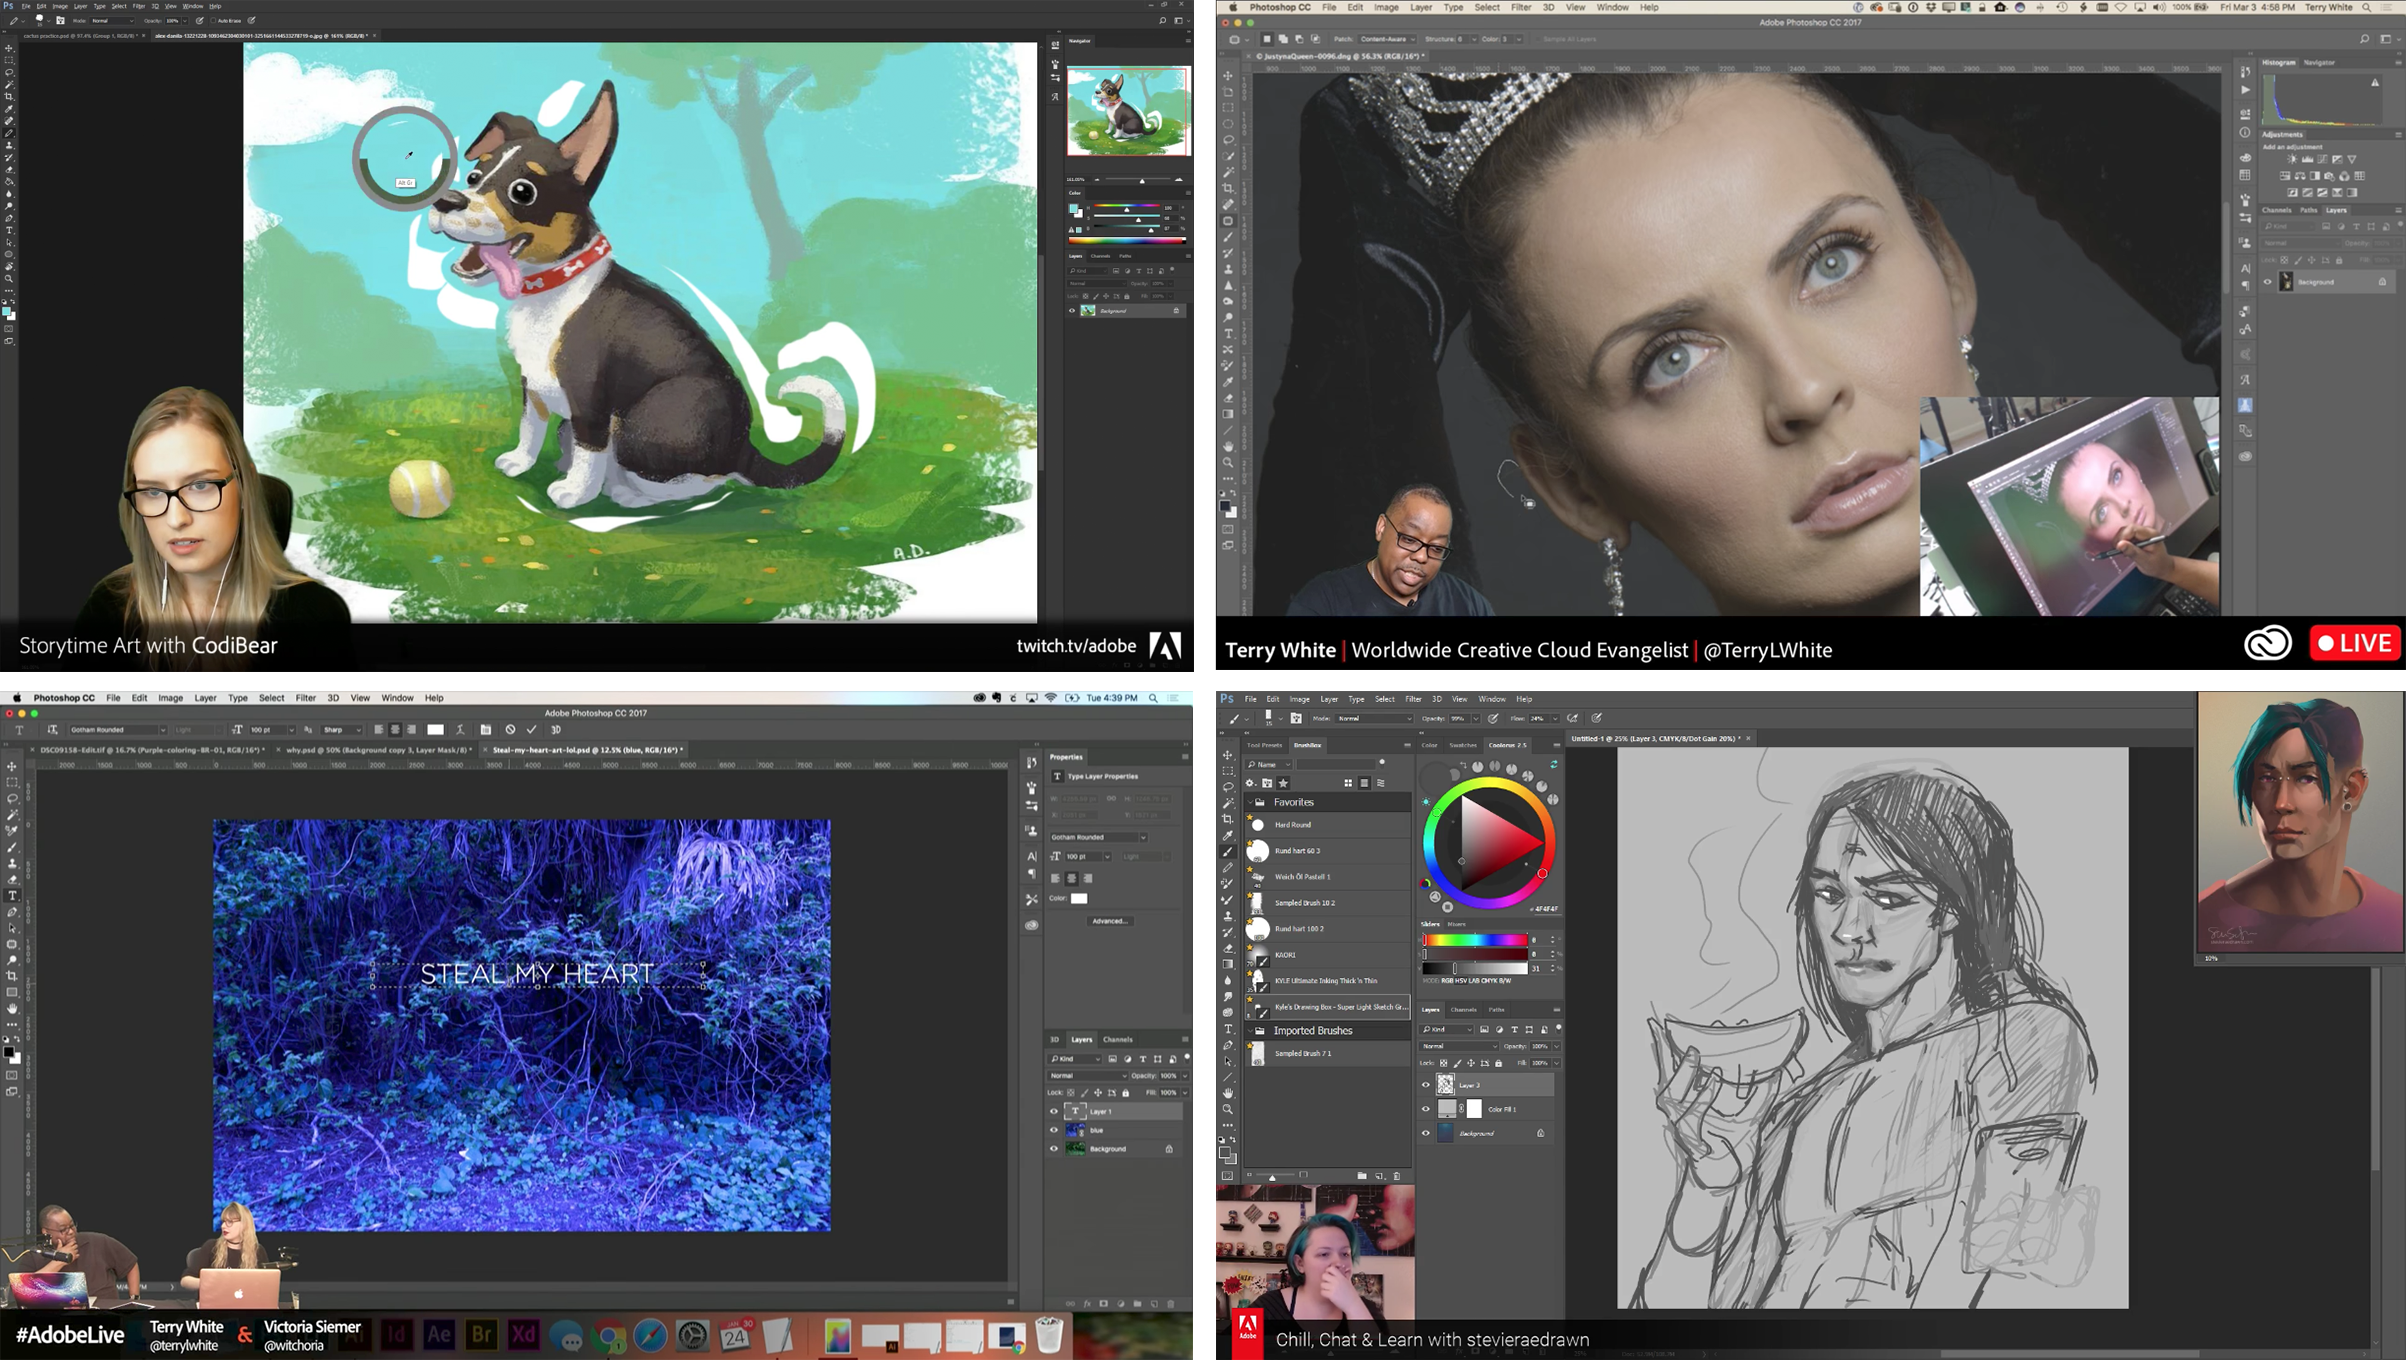
\includegraphics[width=\columnwidth]{liveclips/figures/streamers.png}
  \caption{Examples of creative live-streams on Twitch and YouTube. Artists stream videos of themselves working on creative projects such as graphic design, illustration, and photo editing. (Sources for video screenshots: top left\protect\footnotemark, top right\protect\footnotemark, bottom left\protect\footnotemark, bottom right\protect\footnotemark)}~\label{fig:liveclips_streamers}
\end{figure}

\subsection{Segmenting videos to make them more browsable}
This work uses videos as the source for inspirational examples. Videos have the advantage over text and static images that they show the process of using a tool, rather than just the outcome, and they provide visual demonstrations that are directly relatable to the visual user interface \cite{Grossman2010a}.

Extensive prior work has explored automatically generating educational video clips from screencast videos of software use \cite{Pongnumkul2011, Chi2012, Banovic2012, Lafreniere2014, Nguyen2015}. Though some methods rely on matching telemetry data for these videos \cite{Grossman2010, Lafreniere2014, Chi2012}, others have shown that computer vision alone can be used to detect tool selection events when such data is not available \cite{Pongnumkul2011, Banovic2012}. In this work, we use telemetry data to segment live-streamed videos into clips and rely on computer vision for the presentation and ranking of clips. 

Given a long video with associated tool data, prior work suggests techniques for extracting clips that demonstrate particular tools \cite{Pongnumkul2011, Chi2012, Lafreniere2014}, and guidelines for selecting clips with the best learning value \cite{Lafreniere2014}. Lafreniere et al.'s recommended guidelines \cite{Lafreniere2014} include keeping clips short (15-25 seconds), using clips that show clear visual change to the document, and avoiding clips that show multiple unrelated actions. RePlay builds on this approach to extract and rank clips from live-streamed videos and explores how the characteristics of an inspiring clip might differ from that of an instructional one.

\section{Formative Work: Understanding Creative Live Streams}
\label{sec:liveclips_formative}
Creative live streams are a unique and rapidly growing source of data that have yet to be deeply studied.  To understand the current landscape of creative live streams as well as their applicability to inspiration in software, we conducted content analysis, interviews, and surveys, exploring the following three questions:

\begin{enumerate}
    \item \textbf{What are creative live streams?} For a general sketch of creative live streams, we present a content analysis of a sample of live streams that illustrates the range of content people stream and the different types of creative live streams.
    \item \textbf{Why and how do people stream creative work?} Which parts of their process do they stream? To understand streamers' motivations, processes, and challenges, we present findings from interviews with 8 creative streamers and compare their experiences with streamers in other domains.
    \item \textbf{Why do people watch creative live streams?} To understand the audience these streamers reach, we present findings from three online surveys with 165 viewers that highlight learning and inspiration as key motivators, with entertainment and community close behind.
\end{enumerate}

We found that viewers often seek to learn and be inspired from creative live streams. Notably, inspiration is a much more prominent theme compared with prior work in other live streaming domains such as gaming. However, many streaming platforms are not designed to support these goals, and watching archived streams is tedious. These findings further motivate our goal to make live streams available to users in the context of their own workflows.

\subsection{What Are Creative Live Streams?}
Live stream videos (\autoref{fig:livestreaming_view}) typically show the artist's full screen (when working on a computer) or workspace (for physical work) and a camera view of their face. Live streams usually also feature a live chat, allowing viewers to communicate with each other and the artist. 

There are two main things that make live streamed videos different from other types of videos demonstrating creative work, such as tutorials. First, live streamed videos usually show a real-world process, imparting both creative and procedural knowledge, while tutorials often show contrived tasks, and impart mainly procedural knowledge \cite{Torrey2007}. Second, artists often start without an exact goal in mind, and it can be inspiring to watch someone go from a blank canvas to a beautiful piece of work, though this also means watching the less ``glamorous'' parts of the creative process such as silent thinking or tedious, repetitive tasks.

To learn more about creative live streams, we studied two popular platforms: Twitch and YouTube. As these large platforms cover many types of content, we narrowed our investigation to the \textit{Creative} category on Twitch and the \textit{Adobe Live} video series on YouTube. Through this, we see how streams and communities differ across platforms.  

\begin{figure}[b!]
\centering
  \includegraphics[width=0.7\columnwidth]{liveclips/figures/livestreaming_paper_figure_anonymized.jpg}
  \caption[A typical creative live stream setup.]{A typical creative live stream setup. (a) A camera or screencast displays the artist's workspace. (b) A second camera shows the artist's face. (c) Graphical overlays provide ambient information about the artist (\textit{e.g.}, social media pages) and display interactions with the audience (\textit{e.g.}, pop-ups that appear when viewers subscribe or donate to the stream). (d) Live chat allows viewers to communicate with the streamer. }~\label{fig:livestreaming_view}
\end{figure}

\subsubsection{Creative live streams on Twitch: Content analysis}
To better understand the format and content of creative live\-streams, we analyzed a sample of videos on Twitch, one of the most popular platforms for live streaming. For each creative category, we gathered aggregate metrics about streamers and viewers. We watched and took notes on a sample of 29 videos. We identified four common types of creative live streams that will appear throughout the chapter: \textit{Teaching}, \textit{Making}, \textit{Socializing}, and \textit{Performing}.

\textbf{Methodology:}
To measure the popularity and activity in each of the six creative categories, we queried the Twitch \textsc{api} 4 times a day for 7 days to obtain the number of currently-live streams and number of currently-watching viewers in each category.

We also used the Twitch \textsc{api} to download metadata about the videos in each category (limited to top 600)
%Because this \textsc{api} halts video requests after 600 videos, so our script downloaded metadata for the 600 most-viewed videos in each category. The script 
and randomly selected 50 archived English live stream videos. Four annotators (including the first author) watched each of these videos. Ten videos were not available for viewing and thus excluded (either because their archive expired between being downloaded and being annotated, or because they were only available to subscribers of a channel). Another 11 videos were excluded as they showed video games, TV show reruns, or live event coverage. While these videos were categorized as creative on Twitch, they did not reflect our definition of creative work, namely the creation of a novel artifact. This yielded 29 videos. For each, annotators took notes in a structured spreadsheet on the content presented, camera setup, overall structure of the stream, artist's presentation style, and chat activity.

\begin{table}[t]
\centering
\caption{Summary of popularity of Twitch's creative live stream categories. The number of currently-live streams and currently-watching viewers were collected 4 times a day for a week and then averaged.}~\label{table:livestream_summary}
\begin{tabular}{llll}
\textbf{Category}        & \textbf{\begin{tabular}[c]{@{}l@{}}Avg. \#\\ live streams\end{tabular}} & \textbf{\begin{tabular}[c]{@{}l@{}}Avg. \# live\\ viewers\end{tabular}} & \textbf{\begin{tabular}[c]{@{}l@{}}Avg. \# viewers\\ / stream\end{tabular}} \\
Art                      & 339                                                                    & 6417                                                                    & 21                                                                          \\
Beauty \& Body Art       & 5                                                                      & 177                                                                     & 17                                                                          \\
Food \& Drink            & 19                                                                     & 1088                                                                    & 64                                                                          \\
Makers \& Crafting       & 40                                                                     & 680                                                                     & 16                                                                          \\
Music \& Performing Arts & 286                                                                    & 6881                                                                    & 24                                                                          \\
Science \& Technology    & 91                                                                     & 1155                                                                    & 12                                                                         
\end{tabular}
\end{table}

While this sample does not capture all types of creative activities one might live stream, our hope is that by analyzing a set of canonically creative activities we can shed light on a broader set of activities that might also have a creative component (\textit{e.g.}, video games that involve creating artifacts).
%There is overlap among categories on Twitch, even sometimes within a single live stream when an artist switches back and forth between creative work and other activities like gaming. 

\textbf{Results: Most streamers focus on work \& engage with viewers:}
\autoref{table:livestream_summary} shows overall metrics for the creative categories on Twitch. The most popular categories by far are \textit{Art} and \textit{Music \& Performing Arts}. The category with the most viewers watching per stream is \textit{Food \& Drink}, likely because there are fewer streams to choose from relative to the number of interested viewers. These communities are small relative to the most popular games; for example, the game Fortnite has between 5,000 and 10,000 streams live on Twitch at any given time, with around 100,000 total viewers watching. %\xxx{xxx says move earlier but where?}

\begin{table}[t!]
\centering
\caption{Creative activities shown in a random sample of 29 live streams from Twitch's creative categories, and the primary type of structure each stream exhibits.}~\label{table:livestream_activities}
\begin{tabular}{lll}
\textbf{Category}        & \textbf{Activity (\# videos if \textgreater 1)} & \textbf{\begin{tabular}[t]{@{}l@{}}Primary type\\ of stream\end{tabular}} \\
Art                      & Multimedia production                           & Making                                                                    \\
                         & Digital drawing (4)                             & Making                                                                    \\
                         & Animation                                       & Teaching                                                                  \\
                         &                                                 &                                                                           \\
Beauty \& Body Art       & Makeup                                          & Socializing                                                               \\
                         & Makeup (3)                                      & Making                                                                    \\
                         &                                                 &                                                                           \\
Food \& Drink            & Cooking                                         & Teaching                                                                  \\
                         &                                                 &                                                                           \\
Makers \& Crafting       & Making foam props                               & Teaching                                                                  \\
                         & Sewing quilts                                   & Socializing                                                               \\
                         & Bead art (2)                                    & Making                                                                    \\
                         & Assembling models                               & Making                                                                    \\
                         & Assembling models                               & Socializing                                                               \\
                         & Woodworking                                     & Making                                                                    \\
                         & Pottery                                         & Making                                                                    \\
                         &                                                 &                                                                           \\
Music \& Performing Arts & Music production                                & Performing                                                                \\
                         & Music production                                & Making                                                                    \\
                         & Acting \& improv games                          & Performing                                                                \\
                         &                                                 &                                                                           \\
Science \& Technology    & Building a computer                             & Making                                                                    \\
                         & Programming (3)                                 & Making                                                                    \\
                         & Game development (2)                            & Teaching                                                                  \\
                         & Talking about technology                        & Socializing                                                              
\end{tabular}
\end{table}

The videos span a range of creative activities (\autoref{table:livestream_activities}). The average video length was 3h46m, not including time spent gaming -- a few artists combined both creative work and video gaming into one stream, spending the first part on creative work then switching to gaming when they were finished. The shortest video was 1h3m; the longest was 7h56m. These videos are notably longer than most non-live-stream videos.

Almost all videos contained either a screencast view for work being done on a computer (13/29) or a camera view for physical work (15/29). One showed a distant camera view of the artist producing music in a studio. Most (26/29) showed the artist's face: in 10 as part of the main camera feed, and 16 as a separate feed overlaid in a corner (as in \autoref{fig:livestreaming_view}). Almost all artists (27/29) talked out loud while streaming; of the two silent streamers, one occasionally posted in the chat. Most artists talked about a mix of their work and other topics (18/29). Some talked only about their work (9), or only about other topics (1). One was a variety show, so the talking \textit{was} the work. Many videos (19/29) included background music. 

Most artists engaged with the chat at least sometimes (24/29). 18 artists engaged frequently with the chat, and 6 occasionally. Three videos did not show a chat replay despite the artist referring to the chat; we assume it was not saved or had been hidden. In all 26 remaining videos, viewers asked questions at least occasionally, or in some videos (9/26) frequently. In half of these videos, all chat questions appeared to get answered; in the rest, some (7/13) or many (4/13) questions went unanswered. In 2 videos, most chat questions were answered by other viewers or moderators in the chat.

\textbf{Four common types of creative live streams:}
We identified four common types of creative live streams. We also observed these in interviews with streamers in the next section. Sj{\"{o}}blom \textit{et al.} \cite{Sjoblom2017a} offer a similar characterization of video game live streams; we found some key differences and fewer overall types of structures. \autoref{table:livestream_activities} shows the primary type of each stream in our sample set. These are general high-level trends; some streams bridge multiple types.

\textbf{Teaching} streams have an instructional focus, where the stream\-er is educating the viewers. These include step-by-step how-to demonstrations of tasks such as cooking a recipe, producing a photo-editing effect, or creating DIY costumes. Other examples include critiquing others' work, answering viewers' questions, or explaining a topic.

\textbf{Making} streams focus primarily on creative work and process, but not explicit teaching. These include an artist silently drawing, a streamer attempting a new task they have not tried before and talking their way through it, and an artist making pottery and describing \textit{what} they are doing but not \textit{how}. 

\textbf{Socializing} streams feature the streamer chatting casually with viewers, often while working on a project, such as makeup or sewing (but the project is not the main focus). These are often described as ``chill'' streams. Socializing streams often have tight-knit communities; the streamer will recognize the names of viewers in the chat and ask them how they are doing.

\textbf{Performing} streams feature the artist performing their work. Naturally, these mostly include performative arts like music and acting (\textit{e.g.}, as opposed to drawing). Like with Making, the focus is on the artist's work; in this case the artist does not talk about what they are doing, they just do it. Performing streams differ from non-live recordings in that they often take a more casual improvisational form, rather than scripted performance (\textit{e.g.}, musical ``jam sessions'' or improv acting).

Within each type, the amount of interaction between the stream\-er and the audience varies. Some streamers hold ``request streams'' or ``Q\&A streams'', where the content and flow are determined by audience requests or questions, respectively. Some hold contests or games. A request stream could have audience members requesting songs for a Performing stream, a topic for a Teaching stream, or a particular artifact for the artist to make in a Making or Socializing stream. 

\subsubsection{Creative live streams go professional}
While many live streams are run by individuals, professionally-run streams are also growing in popularity. Adobe, a company that produces creative software, hosts live streams on a regular schedule multiple times a week\footnote{\href{https://behance.net/live}{\nolinkurl{behance.net/live}}}. These can be viewed on Behance or on Adobe's Creative Cloud YouTube channel. They host two live stream series: \textit{Adobe Live} is a Making stream that happens for 6 hours (three 2-hour sessions) three days a week, and it features guest artists usually hosted by someone who works at Adobe. \textit{Daily Creative Challenges} is a Teaching stream that happens for 30 minutes five days a week. It complements contests organized by Adobe to teach new skills. YouTube reports these streams having between 2,000 and 8,000 views each; it does not distinguish between live and replayed views.

\stepcounter{footnote}
\begin{figure}[b!]
\centering
  \includegraphics[width=0.6\columnwidth]{liveclips/figures/adobelive.png}
  \caption{The \textit{Adobe Live} series features a guest artist (bottom left) and a host (bottom right). The artist is working on a digital drawing, and the host is looking up at the live chat feed, engaging with the audience (\href{https://youtu.be/yYDmQhg_1uE}{\nolinkurl{youtu.be/yYDmQhg_1uE}}). }~\label{fig:livestream_adobelive}
\end{figure}

\textit{Adobe Live} differs from most streams by featuring two people. Typically there is a host and an guest artist (\autoref{fig:livestream_adobelive}), but sometimes two artists work together. Adobe hosts different artists every week across a range of creative disciplines (\textit{e.g.}, graphic design, UX design, photography, video editing). Typically, the host moderates the stream, responding to chat messages and passing on questions from viewers to the artist so that the artist can focus on their work. When the stream includes two artists, they trade off hosting.
%xxx: removing for now because we haven't talked about challenges for streamers yet
%These live streams address some of the challenges self-streamers often face, such as facilitating the chat while working and dealing with technical setup, by having separate people take on those tasks. 
The featured artists are usually practitioners, not teachers; their work mainly serves as inspirational demonstrations, while also giving the the community a chance to engage with questions and comments. 

The \textit{Daily Creative Challenges} series features one person who both reads chat messages and provides a short tutorial on a software technique. These live streams are part of Adobe's Creative Challenges, which are contests that encourage people to use Adobe software and submit design work for prizes\footnotemark. These streams are 30 minutes long -- this is short for a live stream -- and focus on instruction: explaining the challenge of the day and teaching viewers the skill of the day. 

\footnotetext{\href{https://www.behance.net/dailycreativechallenge}{\nolinkurl{behance.net/dailycreativechallenge}}}

%The interviews and surveys in this paper are with a mix of people from Adobe's live streams and from other creative communities, allowing us to gain a broad understanding of the challenges creative streamers face and suggest possible improvements for them.

\subsection{Why \& How do People Stream Creative Work?}
%Now that we have a broad understanding of two popular creative live streaming communities, we seek to go deeper into the motivations and processes behind creative live streamers. 
What motivates people to live stream creative work? What challenges do they encounter in the process, and how do these compare with streamers in other domains? We interviewed 8 creative streamers and found that streamers were primarily motivated by sharing and engaging with their audience. However, they find it difficult to connect with their audience while focusing on their work. Additionally, for many, live streaming requires significant effort and behind-the-scenes preparation. 

%Streamer motivations and processes seem to be highly dependent on the type of stream they create. Prior work has shown that the main reasons gaming streamers stream are to build a community of like-minded individuals \cite{Hamilton2014, Pellicone2017} and to make money or promote their personal brand \cite{Pellicone2017}. People who live stream about their lifestyle or to entertain do it primarily for personal branding \cite{Tang2016}. In contrast, educational or culture-sharing streamers' main goal is usually to share their knowledge and culture with others \cite{Lu2018a, Lu2019}. As for process, some live streams are highly produced and require significant preparation beforehand (\textit{e.g.}, e-sports tournaments), while others occur on-the-spot whenever the streamer decides to go live (\textit{e.g.}, many lifestyle streams on Instagram).
%Such streamers often care more about making a broad positive impact and raising awareness about their particular activity than making money or receiving gifts from viewers, even when they do also make money as a side benefit \cite{Lu2019}. 
%We echo Lu \textit{et al.}'s \cite{Lu2019} finding (maybe) that for many types of creative activities that are usually solitary (e.g., playing a solo musical instrument or doing visual art), streaming allows people to have company while they work so the activity is not so lonely.

\begin{table*}[t]
\centering
\caption{Self-reported background information about the eight creative streamers we interviewed. ``Skill'' refers to the streamer's skill at the type of creative work they stream. After interviewing the streamers, we determined the structure type of their most frequent streaming style.}~\label{table:livestream_streamers}
\resizebox{1\textwidth}{!}{
\begin{tabular}{llllllll}
            & \textbf{Role}                                                                       & \textbf{Content}       & \textbf{Skill} & \textbf{Frequency} & \textbf{Platform}                                                              & \textbf{Primary type} & \textbf{Moderators} \\
\textit{P1} & Freelance Digital Illustrator                                                       & Digital Illustration   & Expert         & 3 times / week     & Twitch                                                                         & Making                & Yes        \\
\textit{P2} & \begin{tabular}[t]{@{}l@{}}Video Editor \& Educational\\ Content Maker\end{tabular} & Q\&A, Analyzing Videos & Expert         & Occasional         & YouTube, Instagram                                                             & Teaching              & Yes        \\
\textit{P3} & Artist / Musician                                                                   & Music Improvisation    & Expert         & Occasional         & Facebook, Instagram                                                            & Performing            & No         \\
\textit{P4} & Drawing Hobbyist                                                                    & Digital Drawing        & Intermediate   & Monthly            & Twitch                                                                         & Making                & No         \\
\textit{P5} & Drawing Hobbyist                                                                    & Digital Drawing        & Intermediate   & Monthly            & Twitch, previously Picarto                                                     & Making                & No         \\
\textit{P6} & Adobe XD Evangelist                                                                 & UX Design              & Expert         & Daily - Weekly     & \begin{tabular}[t]{@{}l@{}}YouTube, Facebook,\\ previously Twitch\end{tabular} & Teaching/Making       & Yes        \\
\textit{P7} & Adobe XD Evangelist                                                                 & UX \& Graphic Design   & Expert         & 3 times / week     & \begin{tabular}[t]{@{}l@{}}YouTube, Periscope,\\ Facebook\end{tabular}         & Teaching/Making       & Yes        \\
\textit{P8} & Adobe Designer                                                                      & UX \& Graphic Design   & Expert         & Daily - Weekly     & YouTube, previously Twitch                                                     & Teaching/Making       & Yes       
\end{tabular}
}
\end{table*}



\subsubsection{Interview methodology}
We recruited 8 streamers (4 male, 4 female, ages 20-45) from personal and professional connections for one-hour semi-structured interviews. We interviewed people across creative disciplines and experience with streaming (\autoref{table:livestream_streamers}). We asked participants about their current position and background, process and motivation for streaming, challenges and successes they have experienced, and strategies for engaging with their audience. Three of the participants also host for \textit{Adobe Live}; we asked them about their experience hosting as well as streaming. We took notes and recorded every interview, and analyzed them by comparing participants' answers and identifying common patterns. Interviews were conducted over video chat (4), audio chat (2), or in person (2). Each participant received a \$15 gift card for their time. 


\subsubsection{About the streamers}

\textit{P1} is a freelance artist who began streaming her work full-time on Twitch in 2016. For the first two years, she streamed for 20-25 hours a week and spent the rest of her time on stream-related preparation. At this commitment level, streaming was her primary source of income. Income on platforms like Twitch mainly derives from ad revenue, viewer subscriptions, and donations. Over time, this became exhausting and felt unsustainable. \textit{P1} took a break, and now streams casually 3 times a week but not as a primary source of income. Her live stream setup includes a camera view of her face, a screencast of her work, a Stream Deck (\autoref{fig:livestream_streamdeck}), and two monitors for her to see chat activity and other information.

\begin{figure}[b!]
\centering
  \includegraphics[width=0.5\columnwidth]{liveclips/figures/streamdeck.png}
  \caption{The Stream Deck is a programmable control pad used by many streamers, including \textit{P1}, for easy access to common shortcuts and actions. It integrates with Open Broadcaster Software (OBS), a program used by many streamers to host their live streams (\href{https://www.elgato.com/en/gaming/stream-deck}{\nolinkurl{elgato.com/en/gaming/stream-deck}}).}~\label{fig:livestream_streamdeck}
  \vspace{-0.2in}
\end{figure}

\textit{P2} is a video editor and creator who has been making video tutorials on photo and video editing for about 7 years. He hosts a podcast where he interviews people about their creative approach and life stories. He has tried Periscope, and began streaming on YouTube when it enabled mobile streaming in 2017: casual streaming was on the rise. Occasionally he live streams on YouTube or Instagram, answering viewer questions, teaching a particular topic, analyzing a popular video, or critiquing viewers' work. His setup comprises a camera view of his face, a screencast of his work, and a large monitor for him to see chat activity and other information.

\textit{P3} is a musician who live streams on Facebook and Instagram (with three band members). Her streams are spontaneous and improvisational; the quartet does not play together regularly but they have a fan base that they stream to whenever they are together. These streams require little setup; they are broadcast from a single mobile phone either held by a friend or propped up. She also occasionally streams product reviews and behind-the-scenes views of her shows.

\textit{P4} and \textit{P5} are hobby artists who stream digital drawing about once a month on Twitch. They both started streaming 2 or 3 years ago. \textit{P5} used to stream on Picarto, and moved to Twitch about a month ago because it was easier to use and tends to attract more viewers as a better-known platform. \textit{P5} rarely talks out loud during her streams (only when nobody else is home) and \textit{P4} never does. Instead, they engage with viewers by typing in the chat. Neither shows their face when streaming; their setups include only a screencast of their drawing window. 

\textit{P6}, \textit{P7}, and \textit{P8} stream as part of their jobs at Adobe by hosting artists, streaming their own work, and teaching Adobe products.
%are all employees of Adobe who regularly stream on Adobe's Daily Creative Challenges, and also host on Adobe Live. 
%These participants stream frequently as part of their jobs, and are all highly experienced at the creative work they stream. 
\textit{P6} has been making video tutorials on photo editing for over 10 years. He briefly tried streaming on Twitch but found that his audience did not transfer over to the new platform. He has been streaming with Adobe for approximately 6 months. \textit{P7} taught courses and training programs on design and illustration software for many years. He has been working at Adobe for 9 years, and streaming with Adobe for about 4 years. 
%\textit{P7} was one of the first evangelists involved in Adobe's live streaming efforts, which started on Twitch.
\textit{P8} is a designer and trained illustrator and has been streaming with Adobe for 4 years. Before joining Adobe, she used to occasionally stream her art process on Twitch. By virtue of live streaming professionally, all three participants have fairly sophisticated technology setups, including a camera view of their face in front of a green screen, a screencast of their computer, several displays for them to see chat activity and other information, and sometimes additional cameras (\autoref{fig:livestream_adobelive_setup}). 

\begin{figure}[t!]
\centering
  \includegraphics[width=0.8\columnwidth]{liveclips/figures/adobelive_setup.png}
  \caption[The technical setup for \textit{Adobe Live}.]{The technical setup for \textit{Adobe Live}. (a) The artist (left) and host (right) sit in front of a green screen, with both computers connected for screencasting. (b) Behind the scenes, at least one person helps with technical support, including setup, testing, and monitoring. (c) The artist and host see a display with the live chat feed, and (d) a display showing how they currently appear in the live stream. }~\label{fig:livestream_adobelive_setup}
  \vspace{-0.2in}
\end{figure}

\subsubsection{Findings}
\textbf{Audience engagement is a primary goal for streamers:}
Like with gaming \cite{Pellicone2017, Hamilton2014} and culture-sharing \cite{Lu2019} live streams, audience engagement is important to creative streamers. All participants said they engage with their audience during streams, despite their different personalities and streaming styles. When asked about their main motivation for streaming, participants mentioned creating a space for people to hang out together, building an audience, sharing their process with others, and engaging in meaningful conversations.

When asked for an example of a rewarding or enjoyable moment, every participant mentioned audience engagement in some way. Three participants mentioned feeling rewarded by gratitude from viewers for inspiration and community. This inspiration goes both ways: \textit{P5} mentioned that she has received valuable feedback from a viewer that helped improve her own work. Two participants valued that \textit{``there's something more authentic about [live streaming] ... it allows me to just be myself more authentically and people can pick up on that, they can understand what you're really about in a way that you just can't express via [other modalities]''} (\textit{P2}). \textit{``There are really no mistakes, there's just honesty''} (\textit{P3}).

A key difference between gaming and creative live streams affecting engagement is the scale of the audience. The average live audience size for our participants ranged from about 5 to 1000, with most sitting at the lower end. Popular streamers of video games such as Fortnite or League of Legends often average audiences of between 2000 and 40,000. This means that creative streamers often feel a tighter personal connection with their viewers, while viewers of gaming streams tend to mostly interact with each other, as the chat goes too quickly for the streamer to keep up \cite{Lessel2017, Hu2017}.

\textit{P7} expressed a desire to offer the audience more diverse interactive experiences beyond just text chat. Currently, gaming live streams sometimes host ``audience participation games'' \cite{Glickman2018}. \textit{P1} often organizes games during live streams, such as contests with prizes, voting on what she should do next, or ``prompt games'' where viewers contribute ideas. \textit{P4} did a ``request stream'', where he drew whatever viewers requested, and \textit{P2} often runs Q\&A-form streams, where he will open an application and just let the audience ask questions. As he put it, \textit{``I want to do what they want to do.''} \textit{Adobe Live} often has giveaways for audience participation, and Adobe hosts a \textit{Daily Creative Challenge}. This kind of engagement \textit{``make[s] it a collaborative thing''} (\textit{P6}), increasing audience investment.

One emerging practice is live streaming portfolio critiques. Like a call-in radio show or newspaper advice column, a few people get direct feedback, and many people benefit through over-the-shoulder learning. This form of learning can be extremely beneficial \cite{Lopez2010}; it is notable that there is a streaming audience that seeks it out. Similar to shows and columns, streamers have the challenge of selecting which submission(s) to critique. \textit{P2} initially handled this with chat but was quickly overwhelmed by the number of messages. To address this, he found and installed a widget\footnote{\href{https://streamlabs.com/widgets}{\nolinkurl{streamlabs.com/widgets}}} to help him select submissions and allow users to pay a small amount to have their work critiqued. While valuable, it takes time and effort to manage such tools. This also exacerbates streaming's already ``fragmented technology ecosystem'' \cite{Lu2019}.

Aside from the three Adobe participants who stream as part of their jobs, none of the participants currently stream as a major income source. Though these participants were not \textit{primarily} motivated by monetary gain, two mentioned that it was a significant secondary benefit, \textit{e.g.}, \textit{P4} said, \textit{``it doesn't matter how good my work gets if I don't actually market myself.''} Many streamers in other domains (especially video games) also aim to grow their audience and make money \cite{Pellicone2017}. \textit{P1}'s sought to eventually be a self-sustaining artist; she emphasized that her primary goal was building the audience and creating a positive community; \textit{``I believe that the audience brings [financial benefits].''} \textit{P3} wished it was easier for viewers to donate. Compensation is possible on some platforms (\textit{e.g.}, Twitch) but requires configuration.

\textbf{Moderators \& hosts alleviate common challenges for artists:}
A big part of engaging with the audience is interacting via the chat window with viewers' questions, comments, and feedback. 
%interesting: this is indirect engagement
Most participants said they sometimes have trouble keeping up with the chat as it requires switching focus from their creative work. This split-attention challenge echoes previous findings for programming \cite{Faas2018} and culture-sharing \cite{Lu2019} streams.
%- Paying attention to chat and interacting with audience while working \cite{Faas2018}, especially when work is not on the computer \cite{Lu2019} \\
%-- Messages distracting from work, especially when lots of viewers \cite{Lu2019}
\textit{P5} even said, \textit{``I usually put a warning beforehand that I'm not the most talkative while I'm drawing but I try to check up on the chat as often as I can.''} For \textit{P3} who streams on  a smartphone, it is even harder to pay attention to chat, as it requires stopping her performance and coming up close to the camera.

Moderators are one way to alleviate this challenge for viewers. In large gaming live streams, trolling is common; many streamers have dedicated moderators whose main role is to ban or time-out people posting inappropriate content and enforce a streamer's community guidelines \cite{Seering2017, Lo2018, Seering2019, YvetteWohn2019}. Trolls are seen less often in smaller live streams, yet still appear; 5/8 participants have dedicated moderators. As prior work has shown  \cite{Lo2018, Seering2019, YvetteWohn2019}, employing successful moderators requires significant preparation; streamers must work with moderators to develop guidelines, and they must constantly work to make sure their judgments align. \textit{P1} and \textit{P2} echoed these challenges: \textit{P1} has spent significant time making a document of guidelines for her moderators. \textit{P2} has not, and as a result finds that their judgments do not always align: \textit{``They might want to ban someone that I think is fine, or they might not ban someone that I think should be banned.''}

While moderators can help enforce basic rules and keep the chat constructive, they usually do not support streamers' \textit{engagement} with their audience. Viewers often have questions, feedback, and suggestions for the streamer; these are easily missed. Some moderators do engage in the chat \cite{YvetteWohn2019} but they require training in order to answer questions on behalf of the streamer (\textit{e.g.}, \textit{P1}'s moderators). In addition, some streamers find it difficult to talk out loud to their viewers: both \textit{P4} and \textit{P5} said they would like to have others to talk with, as they did not want to fill the silence alone; \textit{``I'm mostly intimidated by the idea of me having to fill a lot of void space''} (\textit{P4}). While \textit{P4} used Discord and \textit{P5} sometimes used join.me for voice chat, these require extra work on the part of the streamer, and sit outside of the main live stream platform.

A different facilitation role that Adobe streams employ to address these challenges are \textit{hosts}. \textit{Adobe Live} streams feature paid hosts who keep the artist and audience engaged, help artists feel confident, and help them focus on their work. The host watches chat messages come in, says hi and responds out loud to viewers' messages, and decides which of viewers' questions to ask to the artist. As \textit{P7} put it, the host is the \textit{``representative for the chat.''} Hosts strive to keep viewers engaged by asking the chat questions and including viewers' names when they respond to them. Hosts also strive to keep the \textit{artist} engaged and talking. As \textit{P6} put it, \textit{``the last thing you want is dead silence.''} This can be difficult when the artist is shy or quiet, so hosts have picked up tricks such as asking the artist questions about themselves, choosing questions from the chat that are likely to start a conversation, and switching the feed briefly over to their computer to show a relevant tip or trick.


%xxx: commenting out for now
%- moderators can be co-present or telepresent
%- some streamers sometimes have co-present people (helping, audience, etc)

\textbf{Different platforms bring different audiences:}
Some participants stream on multiple platforms. Some start streaming on one platform and then switch to another. This brought up interesting trade-offs between different types of live streaming platforms. Besides mobile platforms being simpler than desktop, different platforms also bring different audiences. \textit{P6} and \textit{P8} used to stream on Twitch before Adobe's live streaming community started. They explained that Twitch is a general-purpose platform dedicated to live streaming. It attracts people who generally enjoy live streams and may be interested in creative work but are less often professional. On Twitch it's harder to attract people who are less familiar with live streams, perhaps because of unique specific features such as ``emotes''; as \textit{P1} explained, \textit{``if you are in the ecosystem you're really happy with it, and if you're not in the ecosystem it's bizarre.''}

\textit{Adobe Live} is an example of a professionally-managed live\-stream aimed at a company's customers. As a result, it tends to attract aspiring designers and creatives who use the software being shown and want to learn how to produce better work. It also attracts more people who are not familiar with live streaming, as it is shown on platforms that also include other forms of media (Behance and YouTube). A challenge with platforms like this is that \textit{``people might not really get ... why watch a live stream''} (\textit{P2}), as it is not yet widely understood.

Finally, platforms like Picarto focus specifically on \textit{creative} live streaming. These attract viewers dedicated to the topic, which can make conversations more focused. The challenge with specific platforms like these (at least in an era where the phenomenon is still growing) is that fewer people have heard of them, so it can be harder to attract viewers. For this reason, \textit{P5} switched to Twitch. Indeed, Picarto generally has 100-200 streams live at any given time, which is considerably less than the Art section alone on Twitch (which has over 300).

The type of creative work being done also affects the audience. For participants who do visual art such as drawing or use creative software, their streams tend to be of the Making or Teaching type, and their audiences mainly comprise other artists or people interested in learning the skill. For \textit{P3} who streams Performing content on Facebook, her audience mainly consists of friends and fans. These viewers enjoy watching the performance and being a part of live music, but are not necessarily looking to learn music themselves.
 
%\subsection{Streaming often requires setup and preparation}
\textbf{Amount of preparation depends on stream type \& preferences:}
While gaming live streamers can simply turn on their screencast and begin playing a game, creative streaming often requires more preparation. 6/8 participants said they prepare before beginning a live stream. Four of these primarily run Teaching streams; the other two primarily run Making streams. For Teaching streams (\textit{P2}, \textit{P6}, \textit{P7}, and \textit{P8}), the streamers spend time before the stream going over what they will show. For Making streams, \textit{P1} and \textit{P5} spend time on the early stages of their creative work. In addition to preparing content, live streaming (especially on desktop platforms) also requires technical setup. Most participants who stream on desktop platforms said this takes time: setting up cameras and microphones, organizing windows across multiple displays, and testing the output.

Most Teaching streams require some content preparation, much like how course instructors make lesson plans. Socializing streams likely require little-to-no preparation, as the content of these streams is mainly driven by conversation with viewers. For example, \textit{P2} sometimes streams casual Q\&A streams on Instagram, enjoying their spontaneous nature: \textit{``you just go live.''} For Making and Performing, preparation time depends on the streamer. Some streamers also announce beforehand when they will stream so that viewers can plan to tune in.
%i said it better. but dont remember how
For casual Performing streams like \textit{P3}'s, all she has to do is turn on the camera and position it. But rehearsed performances require practice beforehand. \textit{P4} said he typically only plans his Making streams 5 minutes before starting, and will start drawing from scratch on the stream. \textit{P8}, who used to do more Making streams, also did not prepare: \textit{``it's as if I am opening up my sketchbook and my friends are there.''} Other Making streamers like \textit{P1} and \textit{P5} prefer to start their work before beginning a stream.

Several participants emphasized that some activities make for more engaging live streams than others. Both \textit{P1} and \textit{P5} said their streams are most successful when they do initial sketching beforehand, then spend the stream filling it in and coloring. This is because the early ideation stages involve more problem-solving and deep thinking: \textit{``to be able to put that full energy ... to get through the failures and to find the successes -- I can't multitask it.''} \textit{P5} also felt this early stage was less appealing for audiences: \textit{``For a long while they're going to have to look at a blank sheet of white `paper' so they don't really see the sketches right away ... I think that loses their attention.''} \textit{P2}, when asked why he doesn't live stream his video editing process, he said he tried it but it was too difficult to focus: \textit{``when you're video editing you need to listen to music and focus ... when you're streaming you need to be engaging with the chat.''} This echoes previous findings for knowledge-sharing \cite{Lu2018a} and programming \cite{Faas2018} streams; streamers often prepare beforehand to ensure that the content being streamed will be entertaining for viewers and will not require too much focus on the streamer's part. 

% other challenges:
% -- Delay between video and chat \cite{Lessel2017} \\
% - Entertaining both novice and expert viewers \cite{Faas2018}
% - fragmented technology ecosystem, hard to manage everything \cite{Lu2019}
% - narrating while also focusing on work \cite{Faas2018} \\
% -- Balancing entertainment with showing realistic process \cite{Faas2018} \\

\textbf{Permanence of live stream archives affects performance:}
We found that the ability to archive live streams significantly affects how streamers perform. Several interviewees mentioned that attentiveness to viewers of a future recording influenced their choices in the moment. \textit{P7} said he sometimes records learning-focused live streams that are meant to be useful as replays, and he interacts less with viewers during those streams. \textit{P2} often deletes or hides his completed live streams because they look less polished than his regular tutorial videos. 
\textit{P4} and \textit{P5} don't archive their videos, as \textit{``[live streaming is] more of a in-the-moment [thing]''} (\textit{P5}). 



\subsection{Why do People Watch Creative Live Streams?}
Every live stream needs an audience. To understand the motivations and challenges of viewers, we conducted three surveys over 1.5 years with 165 people: two with \textit{Adobe Live} viewers; one with viewers of any creative live streams on the Web. All three surveys were voluntary. We found that creative live stream viewers watch streams primarily for \textit{learning} and \textit{inspiration}; community engagement and entertainment were also popular reasons for watching streams. Compared with prior work on live stream viewers in other domains, inspiration is a much more prominent theme in these survey responses.
%In particular, the unique combination of learning with entertainment and engagement that live streams offer makes them an appealing choice over other types of learning-focused content.

\subsubsection{Survey methodology}
The first survey with \textit{Adobe Live} viewers (\textit{S1}) was posted periodically in the chat and overlaid on the stream for four months (August - December 2017). It asked about viewers' experience with creative software, the reasons they watch creative live streams, what other creative live streams they watch besides \textit{Adobe Live}, and how \textit{Adobe Live} streams could be improved. 98 people completed this survey.

A year later, \textit{Adobe Live} had changed considerably: more frequent streams, more audience interaction, and wider and more regular marketing. In January 2019, we conducted \textit{S2} to gain additional insights about viewer motivations and challenges, focusing especially on the live chat experience. The survey was sent directly to previous winners of Adobe's \textit{Daily Creative Challenges} who also showed up regularly in past chat logs of Adobe streams. 41 people completed this survey.

Finally, to zoom out and capture a broader range of creative live stream viewers, we conducted a third survey (\textit{S3}) with viewers of creative live streams on \textit{any}  platform. The survey was disseminated with a snowball method, via the researchers' personal social media accounts. Participants were required to have viewed creative live streams before, which were defined as ``activities such as visual art (drawing, painting, etc.), crafts, music performance, cooking, DIY projects, programming, etc.'' This survey asked viewers about the streams they watch, motivations for watching them, examples of things they learned from them, what else they do while watching, and on which platforms they watch. 26 people completed this survey.

\begin{table}[t]
\centering
\caption{All platforms listed more than once in at least one survey by respondents when asked where they watch creative live streams.}~\label{table:livestream_platforms}
\begin{tabular}{lcccc}
          & \textbf{\begin{tabular}[c]{@{}c@{}}Survey 1\\ $n=98$\end{tabular}} & \textbf{\begin{tabular}[c]{@{}c@{}}Survey 2\\ $n=41$\end{tabular}} & \textbf{\begin{tabular}[c]{@{}c@{}}Survey 3\\ $n=26$\end{tabular}} & \textbf{\begin{tabular}[c]{@{}c@{}}Total\\ $n=165$\end{tabular}} \\
YouTube   & 40                                                                 & 17                                                                 & 17                                                                 & 74                                                               \\
Twitch    & 9                                                                  & 4                                                                  & 17                                                                 & 30                                                               \\
Facebook  & 5                                                                  & 4                                                                  & 4                                                                  & 13                                                               \\
Periscope & 1                                                                  & 1                                                                  & 2                                                                  & 4                                                                \\
Instagram & -                                                                  & -                                                                  & 6                                                                  & 6                                                                \\
Phlearn   & 2                                                                  & -                                                                  & -                                                                  & 2                                                               
\end{tabular}
\end{table}

\subsubsection{What do people watch, and where?}
The most popular platform overall was YouTube (74), with Twitch second (30) (\autoref{table:livestream_platforms}). This is likely skewed by the fact that \textit{Adobe Live} is on YouTube. \textit{S3} had a smaller sample size but found YouTube and Twitch to be equally popular.

\textit{S3} respondents listed content genres they frequently watch live. Categories that came up more than once were programming (11/26), cooking (6/26), digital art (\emph{i.e.}, digital painting, photo editing) (5/26), music (4/26), physical artwork (i.e. drawing, painting) (3/26), 3D modeling (2/26), and DIY (2/26).

\subsubsection{Viewers watch for learning and inspiration}
Viewers responded similarly about motivations in all three surveys. Despite the differences in sample sizes and populations, this suggests that \textit{Adobe Live} viewers' responses may often align with viewers more broadly. Across all three surveys, learning was the most common reason people chose for watching creative live streams (\autoref{fig:livestream_survey_responses}). While learning has also been found to be an important goal for viewers in other domains such as gaming, the primary goal most often cited in prior work is entertainment \cite{Lu2019, Wohn2018, Lu2018a, Hilvert-Bruce2018, Faas2018, Cheung2011}.
%In culture-sharing live streams people learn creative skills or techniques \cite{Lu2019}. 
This difference may be due to the prevalence of Teaching live streams in creative communities.

\begin{figure}[b!]
\centering
  \includegraphics[width=0.7\columnwidth]{liveclips/figures/survey_responses.png}
  \caption{All three surveys asked why people watch creative live streams, allowing them to select all answers that applied from a list. This figure shows all responses chosen by at least 15\% of respondents in each survey. }~\label{fig:livestream_survey_responses}
\vspace{-0.15in}
\end{figure}

Almost all free-form elaborations on viewer motivation mentioned learning. Unlike tutorials and lecture videos, live streams offer direct interaction with the streamer and other viewers, improving the learning experience \cite{Lu2019, Faas2018}. In this way they go beyond just learning content and catalyze ``mentorship communities'' of people with similar interests \cite{Faas2018}. Learners can follow along like an apprentice in a studio, asking questions in the moment. This ability to see authentic, worked examples from start to finish reveals how the streamer makes decisions and recovers from errors \cite{Faas2018}. Viewers often use the knowledge and techniques they learn from creative live streams to inform their own work, as many \textit{S1} respondents stated in free-form responses. \textit{S3} asked for specific examples; 50\% of respondents provided one. They include adopting new techniques such as photo editing operations, trying out a streamer's creative style for things like musical playing or code commenting, and learning how to achieve a specific goal like fixing a hole in a sweater.


In addition to learning, many also reported watching for inspiration / motivation. With one exception \cite{Cheung2011}, primary work has not reported inspiration as a goal. Cheung \& Huang \cite{Cheung2011} describe ``the Inspired'' as one of nine personas for gaming live stream viewers; watching someone stream the game inspires them to play it themselves. However, a large majority of gaming stream viewers watch for entertainment, learning, or providing commentary. While inspiration can be beneficial in many genres, we believe it is especially salient in creative live streams due to inspiration's value for creative work \cite{Herring2009}.

In both \textit{S1} and \textit{S3}, inspiration was the second most popular motivation for watching creative live streams. In addition, 27\% (26/98) of \textit{S1} respondents specifically mentioned inspiration or motivation in free-form responses. 10\% (10/98) also mentioned that the videos helped increase their own motivation and confidence as artists. As one respondent explained, \textit{``[I] like watching artists work because it takes the mystery out of what they do.''} Another said, \textit{``Watching experts make mistakes gives me confidence.''}

Creative work is often a solo activity, and its nebulous nature can make it hard to stay motivated as an artist, often causing creative ``blocks'' such as writer's block. Watching someone else work can motivate viewers to keep going, as well as give them new ideas to try. Respondents in all three surveys mentioned this in free-form responses. For example, one \textit{S1} respondent said they watch live streams for \textit{``getting myself inspired and hyped before I start working.''} An \textit{S3} participant said, \textit{``It's fun seeing someone else's creative process, and usually motivates me to do my own side projects.''}



%In \textit{S2}, 85\% of respondents said they had watched live streams of a creative activity they would not have otherwise been interested in, indicating that live streams can be a good way to discover new topics.

%not directly trying to learn but more get general creative ideas, motivate them to try their own creative projects, and inspire them to see that anyone can do creative things. 


\subsubsection{Viewers also watch for community and entertainment}
People watch all kinds of live streams for entertainment \cite{Wohn2018, Lu2018a, Hilvert-Bruce2018, Faas2018, Cheung2011}. It may be the streamer's personality or style, the chat, or the content itself. %Even though live streams may have long periods of down time with little activity, their unpredictable nature makes them ``engaging but dull'' \cite{Haimson2017}.
People also watch live streams for community. Viewers often feel emotionally attached to the streamer \cite{Wohn2018, Hu2017}, enjoy connecting and conversing with other viewers \cite{Lu2019, Lu2018, Hilvert-Bruce2018}, and enjoy being able to influence the streamer's content or process in real time \cite{Lu2018a}. Live stream communities often lead to longer-term chat groups on other platforms \cite{Lu2018a, Faas2018}.

All three surveys found community and entertainment to be secondary motivations (\autoref{fig:livestream_survey_responses}), showing that these are also important motivators for creative live stream viewers. Several \textit{S1} respondents valued the company of other creative people while they worked alone. To investigate this further, Surveys 2 and 3 asked what people do while watching live streams (multiple choice). 68\% (28/41) of \textit{S2} respondents said they watch while doing creative work. 69\% (18/26) of \textit{S3} respondents said they watch while working on something, and 31\% (8/26) said they work on a similar task as the streamer. In this way, creative live stream communities offer a virtual co-working space for people who would otherwise be working alone.

Respondents in all surveys specifically mentioned that the \textit{combination} of learning and entertainment was what drew them to live streams. This echoes Lu \textit{et al.}'s findings with knowledge-sharing streams \cite{Lu2018a}: they are appealing because they disseminate knowledge in a more relaxed, casual way than tutorials or lecture videos.


%Finally, people watch live streams for community and social engagement. Viewers of a particular stream share a common interest, and the live chat feature of live stream platforms makes it easy for these viewers to connect with each other as well as with the streamer \cite{Hu2017}. 


\subsubsection{What are the challenges for viewers?}
\textit{S1} and \textit{S2} asked how the viewing experience might be improved. The most popular suggestions had to do with interactivity and engagement between the streamers and the chat. 17\% (7/41) of \textit{S2} respondents said their questions often get lost in the chat. Busy chat feeds are a problem in other types of live streams as well \cite{Miller2017}, but can be especially frustrating for viewers seeking to learn and ask questions. Two respondents in \textit{S1} wished that hosts would interact more with the chat, and three others emphasized hosting skill, saying that the best hosts are able to keep the conversation interesting and interact meaningfully with the audience. Two respondents in \textit{S2} wished there were more ways to involve the chat, \textit{e.g.}, through quizzes or polls. Finally, several respondents mentioned that the experience watching replays could be improved; one \textit{S1} respondent said a summary document with important links and tips could help with reviewing the stream later, and three \textit{S2} respondents wished they could view the chat and somehow be involved in the stream when watching replays. This agrees with Lu \textit{et al.}'s findings \cite{Lu2018} that it can be hard to learn from a stream after the fact, as navigation options are usually limited.

\subsection{Summary of Findings}
This section's surveys and interviews uncovered the many goals and motivations streamers and viewers have for creative live\-streams. We also found that existing platforms do not support all these goals or offer help when goals conflict. Specifically, viewers often seek inspiration from creative live streams, but live stream viewing takes place out of context of the viewer's own work. Moreover, despite the wealth of expert knowledge and inspiration such videos contain, watching them as archives is tedious and difficult. Several survey participants mentioned the viewer experience for watching live stream archives is poor because the videos are long, have limited navigation, and include long periods of downtime and conversation with the then-live chat \cite{Lu2018}. Twitch viewers can create ``clips'' and streamers can create ``highlights'' of interesting moments, but they must remember to do so, and such moments can seem out-of-context when viewed on their own.

Motivated by these findings, the remainder of this chapter explores how we might help creative software users benefit from the wealth of expert knowledge hidden in creative live streams without having to watch all the downtime and unrelated conversation that comes with it. We do this by capturing the moments of insight and inspiration from creative live streams and bringing these moments into the context of creative software users' workflows.
\section{Design Space for In-Application Video Examples}
\label{sec:liveclips_designspace}
To help inform our decisions in developing LiveClips and explore how users might interact with such a system during their creative workflow, we outlined a design space for systems that present contextual video examples (\autoref{fig:liveclips_designspace}). This design space is informed by our formative findings as well as prior work on contextual assistance in software. The following three sections present the LiveClips system, which includes three alternative interfaces that explore three different points in this space. This section also highlights where RePlay and ReMap (Chapters \ref{chapter:replay}-\ref{chapter:remap}) fit in the design space as compared to LiveClips. Most notably, LiveClips differs from RePlay and ReMap in that it presents inspirational content rather than educational, and it presents short tool-focused clips rather than entire task-focused videos.

\begin{figure}[b!]
\centering
  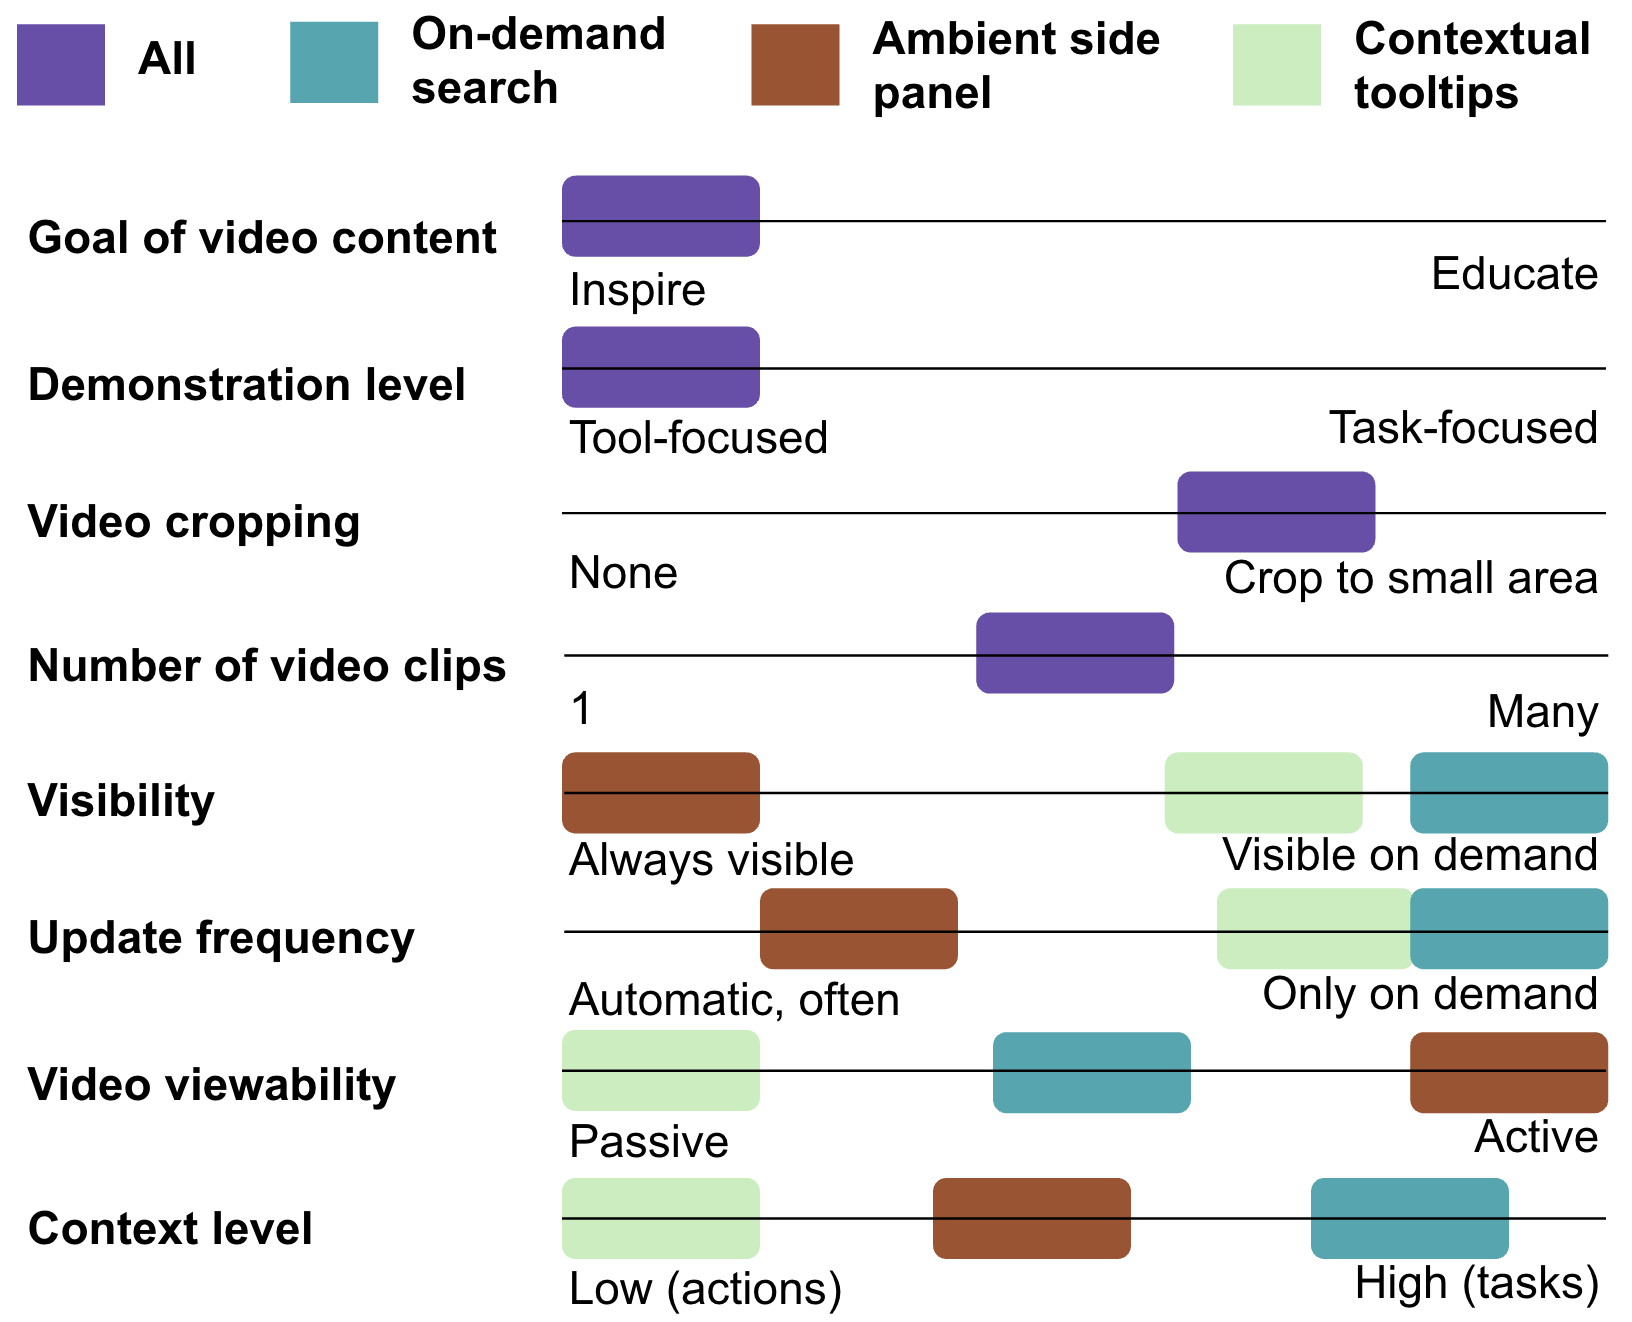
\includegraphics[width=\columnwidth]{liveclips/figures/designspace.png}
  \caption{The design space for in-application video examples, as well as where LiveClips and RePlay/ReMap fit along each axis. LiveClips' prototype interfaces vary along the bottom four axes. }~\label{fig:liveclips_designspace}
\end{figure}

\subsection{Goal of Video Content}
Most prior work regarding contextual videos, including RePlay and ReMap, has focused on content that aims to educate the user, such as tutorials \cite{Pongnumkul2011} and helpful tips \cite{Grossman2010a}. Inspired by the known benefits of examples for inspiration \cite{Kulkarni2014} and our survey findings suggesting that live streamed videos are used for inspiration, this work explores how contextual live streamed videos might inspire users. These videos also have educational value, but this work focuses on them as a source of inspiration.

\subsection{Demonstration Level}
Videos of software use can be tool-focused or task-focused. A tool-focused video demonstrates using a single tool, while a task-focused video shows an entire task from beginning to end.  Tool-focused videos are useful for quick contextual help that does not take away from the user's current work, for example reminding the user how a tool works \cite{Grossman2010a} or showing alternative uses for a tool.
Task-focused videos tend to be longer and are less useful in-the-moment, as they show a specific task that may or may not be relevant. Live streams tend to be task-focused, as they usually follow an artist through an entire task; this work focuses on extracting shorter, more generalizable tool-focused examples from task-focused live streams. RePlay and ReMap also extract relevant moments from within longer task-focused videos, but unlike LiveClips, they are meant for users who proactively seek help with a particular task, so they allow the user to browse the entire video and follow along with it.

%The likelihood that this task will be directly relevant to the user is low \cite{?}. 
%In this work, we focus on creating short tool-focused clips out of longer task-focused videos based on the assumption that shorter bite-sized clips are more useful as in-context recommendation, as they do not take the user away from their current work like a long task-focused clip would. 
%In addition, videos of artists using software often highlight alternative uses for tools that viewers may not have seen before, and so seeing a variety of ways a tool can be used may provide both inspirational and educational value. 

%Many of today's popular creative software applications support a wide variety of workflows. As a result, many of their tools can be used for multiple different purposes and in different contexts. Even expert software users may not be aware of all the different ways a tool can be used. Thus we expect that in addition to providing inspiration, tool-based clip recommendations may help increase users' awareness of the different ways tools can be used. By narrowing in on a focused aspect of a video, we also provide this content in a way that does not detract too much from the task at hand, unless the user wants to see more.

\subsection{Video Cropping}
In-application examples are constrained by space; if content takes up too much space it becomes obtrusive, for example by blocking the canvas where the user is currently working. Therefore, contextual videos must be displayed at a relatively small size. For videos that were created using full-screen video capture (as most live streams are), this can be problematic. Leaving a video un-cropped allows the user to see the full context of interaction but makes it difficult to discern any detail. Since RePlay and ReMap left videos un-cropped, they allowed users to open a single video in a larger window when seeing more detail was necessary. While this may have been practical for task-focused learning where users have other cues to indicate a video's relevance before selecting one (\textit{e.g.}, caption previews), LiveClips aims to show users many examples at once of tool use that may only take place in a small part of the screen. Prior work has explored how to best present video demonstration clips when they cannot be viewed in full screen, by cropping or enlarging sections in the video where mouse movement and canvas changes occur \cite{Chi2012}. Inspired by this, LiveClips crops videos to the area that shows the most visual change, in an effort to make examples focused and easy to browse.

\subsection{Number of Video Clips Shown}
Examples could be displayed one at a time, taking up the least amount of space but also providing less variety. Alternatively, displaying many videos gives users more options but potentially overwhelms them. Prior research on contextual videos recommends displaying multiple videos to demonstrate the range of uses for a tool and increase the likelihood that the user will find at least one useful \cite{Lafreniere2014, Matejka2011}. Similar to RePlay and ReMap (which displayed five videos at a time), our prototypes display four videos at a time in an effort to provide some variety without overwhelming the user or taking up too much space.

\subsection{Visibility}
Examples can be always visible while the user is working (like with RePlay and ReMap), or visible only on demand. Examples that are always visible are more likely to be seen but can be distracting, while examples that are not easily visible and shown only on request are more likely to be ignored or missed \cite{Rhodes1996}. Different users may have different preferences for how visible they want their examples to be, just as some viewers like to watch creative live streams while they work, while others may not. Our prototypes explore three variations along this axis.

\subsection{Update Frequency}
Recommended examples can update in response to an explicit user action (\textit{e.g.}, a query), an implicit user action (\textit{e.g.}, being idle for some time or opening a new document), or automatically at a regular time interval. Updating in response to explicit user actions was appropriate for RePlay and Remap, which are intended to be used when users have a specific question. But for a system like LiveClips that aims to elicit inspiration, the ideal approach is less clear. The trade-offs between these strategies have been widely explored in the literature, and it seems there is no globally optimal solution \cite{Rhodes1996, Chan2017, Siangliulue2015}. Automatic updates can be useful because they require zero effort from the user and can highlight an example in the moment \cite{Rhodes1996}, but they can also distract the user during periods of focused work \cite{Chan2017} or make the interface feel uncontrollable \cite{ODonovan2015}. Updates in response to an explicit request are less distracting and give the user more control over their attention but rely on the user to know when an update would be useful \cite{Rhodes1996, Siangliulue2015}. Update frequency is also tied to Visibility; recommendations that are only visible on-demand only update (visibly) when the user requests them. As with Visibility, the ideal solution may depend on the user's preferences; our prototypes explore three variations.

\subsection{Video Viewability}
When presenting non-static content such as videos in-app, the way in which the user interacts with and views the content may affect its usefulness. On the passive end, videos could play automatically when the content appears, which removes the need for the user to decide whether or not to watch a video but runs the risk of being distracting. On the other end, videos could be shown as a static thumbnail that only animates when the user intentionally interacts. Most prior work  \cite{Grossman2010a, Chi2012}, including RePlay and ReMap, has adopted the latter approach, however such work also suggests that in-context content should have a low threshold for engagement; the user shouldn't have to break too much from their task to interact with recommended content \cite{Grossman2010a}. LiveClips explores three variations along this axis.

\subsection{Context Level}
Examples can vary in how contextual they are to the user's behaviour. Low-level examples respond to the user's individual actions, such as the tools they use. High-level examples respond to the user's task or intent, which can be inferred from sequences of commands or by analyzing the document being edited. RePlay and ReMap use low-level context to augment queries, but the queries themselves can be either low- or high-level depending on the user. LiveClips mostly focuses on lower-level examples, but one of our three prototypes explores a potential way to measure task-level similarity between the user's actions and the examples clip's source video.
\section{LiveClips System Overview}

LiveClips takes as input a live streamed video and telemetry data for the software usage in the video. It extracts short clips showing bite-sized chunks of the artistic process, crops clips to thumbnail size, and ranks clips for recommendation based on their properties as well as the user's context. In the current implementation, audio is removed to focus solely on the visual component of the videos. %(SYSTEM DIAGRAM)

Our approach is tool-centric: each clip focuses on one tool and LiveClips recommends clips based on the user's tool use in the application. We focus on tools as a starting point, because prior work has demonstrated that short tool-focused clips can be effective for contextual learning~\cite{Grossman2010a} and creative software tasks are often centered around the use of different tools.

\section{User Interfaces}
Based on the design space outlined above, we present three alternative methods for displaying and recommending the video clips generated by LiveClips in creative software (\autoref{fig:liveclips_photoshop}).
All three methods provide a link to the original video source underneath each clip, so that users can easily access it if desired. Each interface was implemented as a prototype \textsc{html}/Javascript extension to Adobe Photoshop.

\begin{figure}[t!]
\centering
  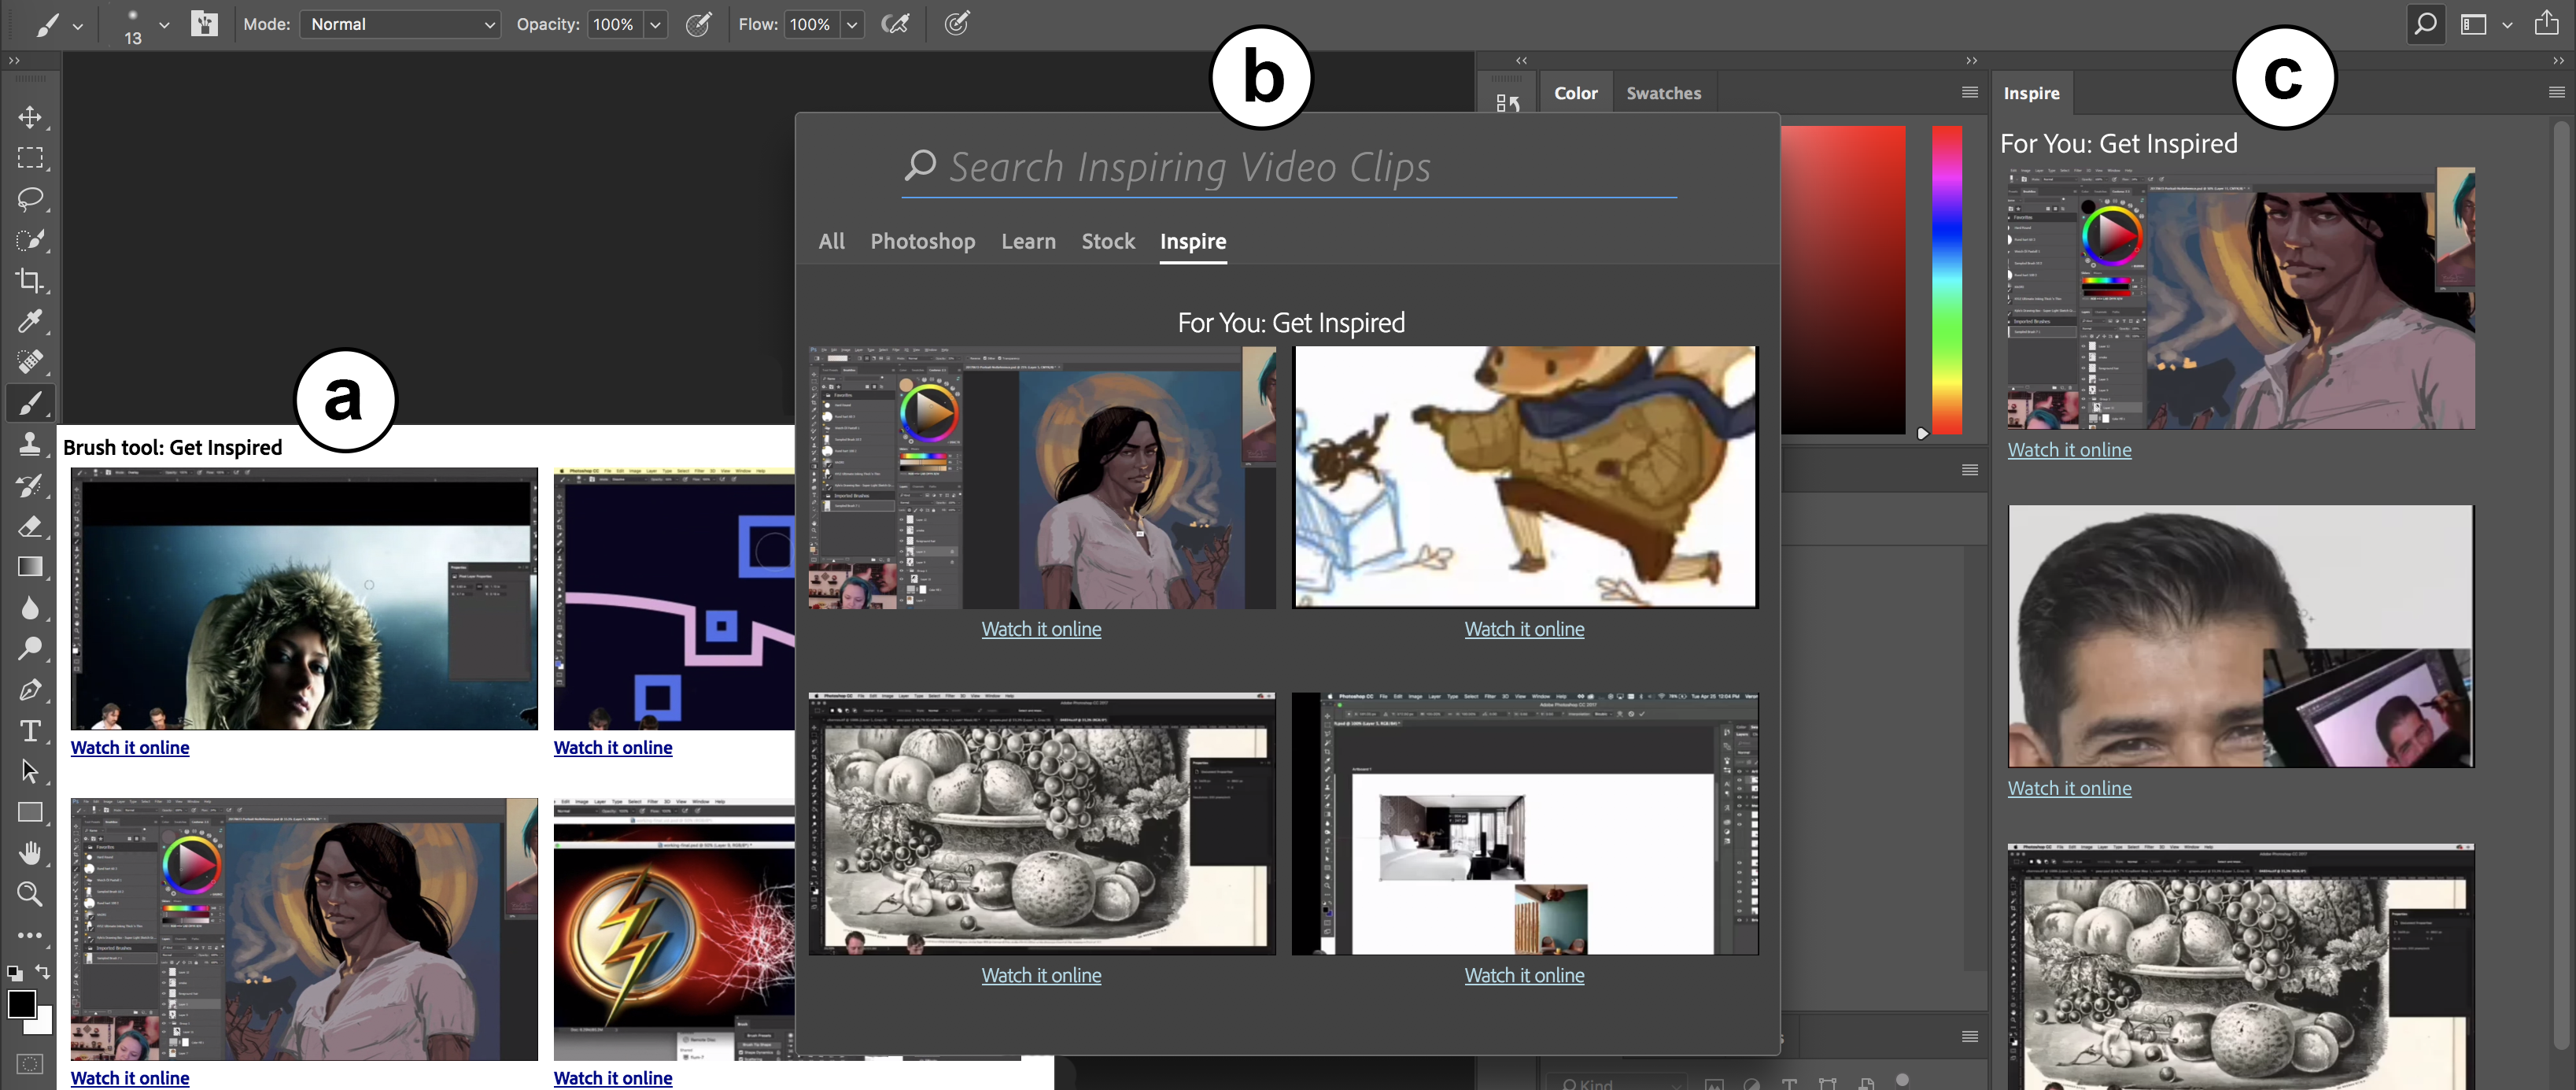
\includegraphics[width=\textwidth]{liveclips/figures/all_interfaces.png}
  \caption[LiveClips' three interface prototypes demonstrate how video clips taken from creative live streams can be embedded in a software tool as inspirational examples, implemented here in Adobe Photoshop.]{LiveClips' three interface prototypes demonstrate how video clips taken from creative live streams can be embedded in a software tool as inspirational examples, implemented here in Adobe Photoshop. a) Contextual tooltips: When hovering over a tool icon, clips of that tool being used are shown. b) On-demand search: Pressing Photoshop's search button or Ctrl-F brings up an extended search interface with task-level clip examples. c) Ambient side panel: an always-visible panel updates periodically with clip examples based on the user's recent tool use. }~\label{fig:liveclips_photoshop}
\end{figure}

\subsection{On-demand Search}
Many software tools provide in-application search, which allows users to search for application features, help, and/or recent documents. We augmented Photoshop's in-application search interface to present four clips when the search window is opened (\autoref{fig:liveclips_photoshop}b). Clips are selected based on the user's tool usage during the entire work session. Users can also search the entire library of video clips from this window. This interface is the closest in concept to RePlay and ReMap's interfaces. As such, we expect this interface to be most useful in moments where the user is stuck and wants new ideas. Each video is displayed as a thumbnail showing the first frame and plays when clicked on.

This interface has low visibility, and updates only in response to an explicit user action. It uses higher-level context to recommend examples. Playback requires intentional mouse clicks.

\subsection{Ambient Side Panel}
Since creative applications tend to include many panels, a natural location for examples is in a side panel. This interface explores examples that update ambiently as the user works (\autoref{fig:liveclips_photoshop}c). To avoid distracting the user during periods of focused work \cite{Chan2017}, the examples only update after the user has been idle for 10 seconds, indicating that they might be taking a break or trying to think of new ideas \cite{Siangliulue2015}. The panel shows four clips based on the user's recent tool use. Mousing over a clip plays it, providing a low threshold for interaction without distracting the user by playing video clips automatically.

This interface has high visibility, updates in response to implicit user actions, and uses mid-level context to recommend examples. Playback requires mouse movement without clicks.

\subsection{Contextual Tooltips}
For an interface that lies between an on-demand window and an always-visible panel, our third approach shows examples in tooltips that appear when the user hovers over a tool icon for 3 seconds (\autoref{fig:liveclips_photoshop}a). Inspired by ToolClips \cite{Grossman2010a}, we believe tooltips may be a useful location for video examples. They can be activated by the user with minimal effort, are easily dismissed, and will not display at all if the user is working quickly or activating tools with keyboard shortcuts.
Tooltips are a natural place for tool-centric examples; the video clips shown are based on the tool selected. Our implementation shows four clips when the user hovers over a tool, and clips play automatically when the tooltip appears.

This interface has mid-level visibility, updates on demand, uses low-level context (tools) to recommend examples, and requires no interaction for video playback. 

\section{LiveClips System for Generating Clips}
The LiveClips system comprises three stages: 1) extracting short 25-second clips based on tool use from long videos, 2) cropping clips so that they can be displayed at thumbnail size, and 3) ranking clips for the three interfaces described above. 

Our approach uses a hybrid of telemetry (recorded usage data) and computer vision to understand and analyze the videos. We note that this could be accomplished entirely with telemetry (as in \cite{Grossman2010, Lafreniere2014}) by instrumenting the artists' software with detailed logging. Conversely, it could be accomplished entirely with computer vision, as prior work has shown that mouse movement and tool selection can be detected from videos alone \cite{Banovic2012, Pongnumkul2011}. In our case (which is not uncommon), we have some usage data that is not fully detailed. Our approach aims to be a catch-all that allows working with a mixed or inconsistent set of data. LiveClips removes all audio from clips during processing, focusing only on the visual component.

\subsection{Available Data}
To develop and test LiveClips, we collected a sample dataset of live streamed videos. In an effort to make the sample as representative as possible, we collected videos from two sources (Twitch and YouTube), from 17 different artists, and for two different software applications: Adobe Photoshop and Illustrator. Videos ranged in length from 30 minutes to 3 hours, giving us a total of 30 hours of video content from 17 different videos. 

For each video we had access to telemetry data at the level of tool usage, which includes time-stamped events for every selection and invocation of a tool (\autoref{fig:liveclips_usage}). Mouse clicks and canvas manipulation details were not available. Our dataset included the use of 36 different tools from the toolbars in Photoshop and Illustrator.  

\begin{figure}[b!]
\centering
  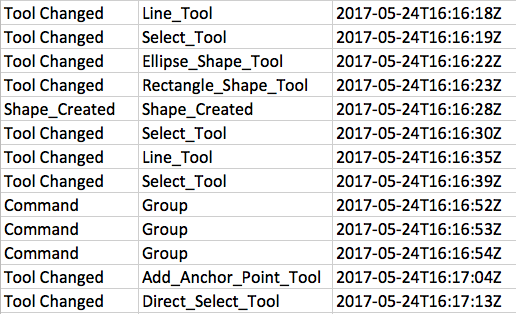
\includegraphics[width=0.5\columnwidth]{liveclips/figures/usage.png}
  \caption{A sample excerpt of the time-stamped usage data we had for each live stream video.}~\label{fig:liveclips_usage}
\end{figure}


\subsection{Extracting Clips}
To extract short clips, we use a heuristic approach based on work by Lafreniere \textit{et al.} \cite{Lafreniere2014}, who segment videos to create instructional clips of tool use. Our focus is on creating inspiring clips, which are different from instructional clips in that they require less attention to specific details (such as setting a tool's parameters) and more attention to the content being created. For the purposes of segmenting initial clips, our method is very similar to Lafreniere \textit{et al.}'s method. We focus on inspirational value in the cropping and ranking stages.

Given a tool, our goal is to create clips showing its use. First, we group all consecutive invocations of the tool and include the tool selection event if it happened within 10 seconds of the first invocation. We add 2 seconds of padding to the beginning so that the viewer can see the tool being selected or invoked. We then trim clips to 25 seconds, as prior work has indicated that 15-25 seconds is a desirable length for in-app video clip recommendations \cite{Lafreniere2014}. We also ignore tool events that are for navigation (\textit{e.g.}, zoom, scroll, select) as these tend to happen frequently in visual software as part of other tasks. We shorten clips where the context likely changed before it was over, i.e. if a document is closed or opened. If a clip is shorter than 15 seconds, we remove it.

This heuristic approach sometimes fails. For example, live streaming artists often work meticulously with one tool for long periods of time (\textit{e.g.}, a brush tool to create artwork), making incremental changes that over time create a more drastic and impressive change. The first 25 seconds of this may not be very inspiring, so we also explore an alternative method for creating clips that brings the focus away from the specifics of a tool's use, and toward the content being created: for instances where a tool is used consecutively for longer than 25 seconds, we extract the entire section where that tool is used, and speed it up to be 25 seconds long. We refer to these as timelapse clips.

In our sample set of 30 hours of video, the above two methods combined produced 1,727 clips, 484 of which were timelapses. This is comparable with Lafreniere \textit{et al.} \cite{Lafreniere2014}, who generated approximately 2500 clips from 25.5 hours of footage. LiveClips generated between 1 and 939 clips for each of the 36 tools in our telemetry dataset.

\subsection{Cropping Clips}
To present examples within an application, they have to be easily viewable by the user. A main design challenge with contextual clip recommendations is the space constraint: prior research has shown that in-app video clips should be unobtrusive and not take up too much of the user's screen \cite{Grossman2010a}. Since live streamed videos typically include the artist's entire screen, simply resizing them to a small thumbnail size will make most of the interesting detail hard to see. Existing methods for cropping videos to a good thumbnail size include cropping it to only the region of the document that changes in the clip \cite{Grossman2010} or cropping to only relevant UI regions \cite{Chi2012}. While more animated effects such as ``pan and zoom'' might be appealing for providing both context and detail, Chi \textit{et al.} \cite{Chi2012} found that too much animation is disorienting for brief video clips.

Since prior work has shown that visible change is an important factor affecting the usefulness of a video clip \cite{Lafreniere2014}, LiveClips attempts to crop each video clip to the area that changes most in the clip, so that the viewer's attention is drawn to the changes that are happening. For inspiration, we are mainly interested in visual change on the canvas. However, there are many other types of visual change that happen in these videos, such as switching windows, opening dialogs, and zooming in and out. Some of these changes (\textit{e.g.}, zooming) are simply uninteresting, and others (\textit{e.g.}, setting parameters in a dialog) may be helpful in a tutorial but are less interesting for short inspirational clips. 
 %The main goal for this content is to expose users to what's possible. Though users might want to see more specifics when they try and follow the artist's method, they will only reach this point if they find the content inspiring in the first place. In such situations, they can click go to the source video and watch the full original video on the Web. 
%
LiveClips therefore excludes these types of change before identifying the area that exhibits the most visual change. This leaves canvas changes and other UI changes. Although we are primarily interested in canvas changes, we leave the task of separating these from UI changes to future work.

To filter out these ``uninspiring'' visual changes, LiveClips uses computer vision to exclude visual change caused by navigational movement, changing application windows, and the artist moving in the webcam view. To detect navigation events, LiveClips does simple feature detection and point feature matching in \textsc{matlab} across consecutive frames to identify and exclude frames where there is a significant amount of motion (likely due to panning or zooming). To detect application window changes, LiveClips identifies moments where more than 90\% of the pixels change between two consecutive frames, and ends the clip before this change occurs. To detect change caused by the artist's webcam view, LiveClips uses face detection in \textsc{matlab} to locate faces that are consistently present in a bottom corner of the screen (which is the customary place for streamers' webcam views) throughout the video, and mask out the corner containing those faces.

To determine the area of most change after filtering out uninspiring changes, LiveClips first calculates the pixel-wise difference between each pair of consecutive frames in the video clip. It then computes the average difference over all of these difference frames. There are many changes around the edges of a clip where artists open menus and panels, but these are not very interesting. The interesting changes are on the canvas, which is typically in the middle of the screen. Thus, LiveClips trims off 100 pixels from all four sides. Next, LiveClips further trims off all sides where the pixel values in the average difference frame are less than a given threshold (which we set to 1/4 of the maximum value in the frame). This allows us to avoid specifying a desired crop size, since some clips may be already zoomed in on the part of the canvas being changed, requiring minimal cropping, whereas others may be zoomed out, requiring substantial cropping to highlight the changing area. \autoref{fig:liveclips_change} shows an example of the average difference frame from a clip and the crop that results from it.
.

\subsection{Ranking Clips for Recommendation}
The set of candidate clips generated is much too large to be useful, as only a few videos will eventually be shown to the user at any given time. As Lafreniere \textit{et al.} \cite{Lafreniere2014} found, over 50\% of automatically selected clips are of poor quality, so choosing good clips from the candidate set is an important step. This section outlines the criteria LiveClips uses to rank clips.

\subsubsection{Time in the original video}
Live streamed videos are several hours long and often show an entire project happening from start to finish. The closer an artist is to the end of their project, the more finished content they are likely to have on their canvas, and thus the more inspiring it is likely to be% (figure showing comparison if time)
. For each clip, LiveClips divides the start time of the clip by the total length of the video to obtain a number between 0 and 1 indicating how far along in the video the clip occurs. Larger numbers are better because they indicate that the clip occurs closer to the end.

\subsubsection{Amount of visual change}
 Lafreniere \textit{et al.} \cite{Lafreniere2014} found that showing clear visual change in short clips was most closely correlated to user preference. To determine how much visual change a given clip shows, LiveClips takes the cropped difference frame generated in the previous stage (\autoref{fig:liveclips_change}), and averages it across the $x$ and $y$ dimensions to obtain a numeric value representing the average amount of change in that clip (a larger number = more change).

\begin{figure}[t!]
\centering
  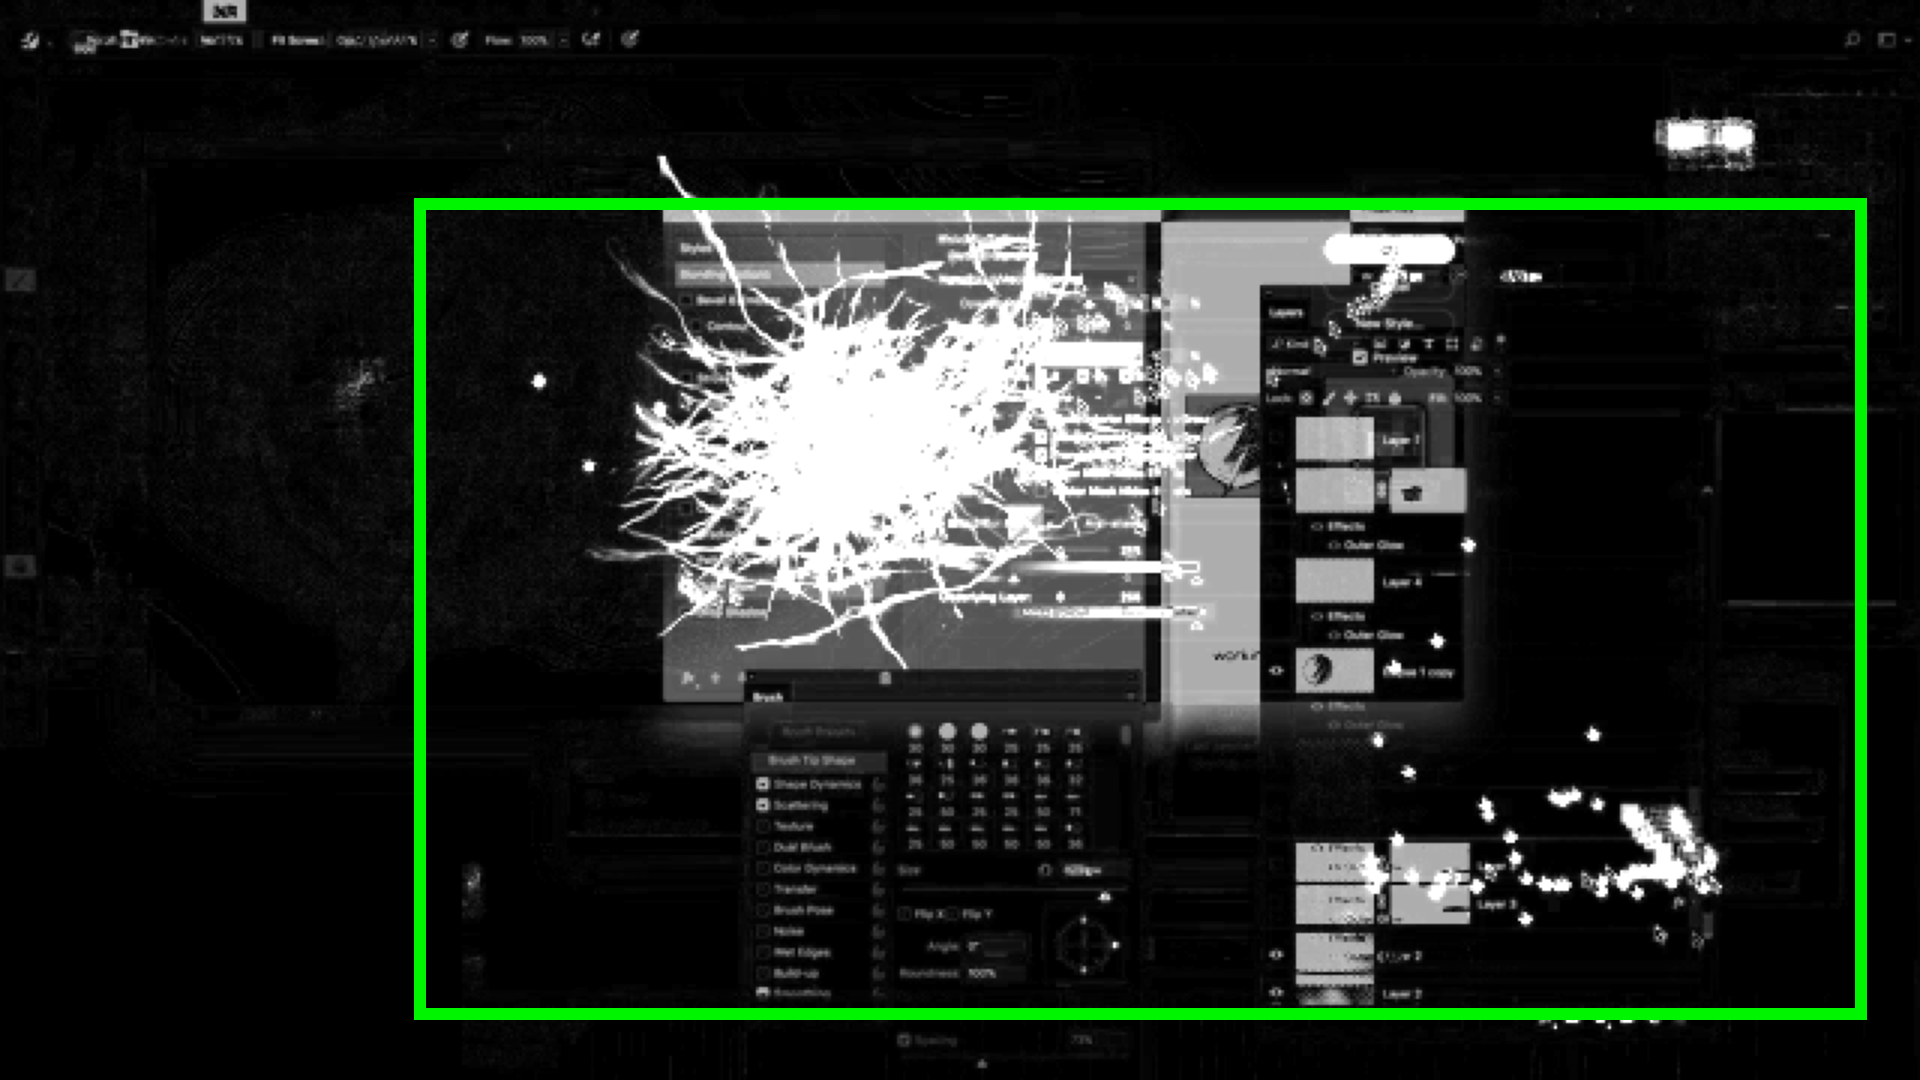
\includegraphics[width=0.7\columnwidth]{liveclips/figures/change.png}
  \caption[An example of a clip's visual change averaged across time (with change caused by navigation, application window switching, and the artist's face moving removed).]{An example of a clip's visual change averaged across time (with change caused by navigation, application window switching, and the artist's face moving removed). From the brightness values of the pixels, we can see that the artist opened some dialogs, and drew some lightning strokes. The green box shows how LiveClips crops the clip to focus on the area that is changing. }~\label{fig:liveclips_change}
\end{figure}

\subsubsection{User context}
User context is the final factor for selecting which video clips to present to the user. This metric varies in each of our three prototypes, to explore different levels of user context. LiveClips' current implementation uses tool use to measure context. LiveClips first calculates a ``total'' score for each clip by normalizing the time and visual change scores from above to be between 0 and 1, then taking the average. (For simplicity, we weight the two metrics evenly.) 

\textbf{Low-level context:} The contextual tooltips interface uses low-level context to recommend examples; video clips are selected based on the tool that the user hovers over. For a given tool, LiveClips orders all clips of that tool by total score, then picks the top four clips. LiveClips requires that all examples come from different source videos, to ensure a variety of content. If some of the top examples are from the same original video, the system goes down the list until it has a set from four different source videos. %In practice, this rarely happens. 

\textbf{Mid-level context:} The ambient side panel uses mid-level context to recommend examples; video clips are selected based on the last four tools the user has used. For each of those tools, LiveClips chooses the clip with the highest total score. If some of these clips are from the same original video, LiveClips instead picks the next top clips that are from different videos, to ensure variety.

\textbf{High-level context:} The on-demand search interface uses high-level context to recommend examples; the user's entire session of tool use is taken into account as well as the entire video from which each clip was extracted. %Many tools can be used for a variety of tasks; for example the brush tool in Photoshop could be used for making a digital painting, or for brushing on a mask to edit a photograph. It is likely that the overall distribution of tools used differs for the above two tasks: a user making a painting would likely spend most of their time using the brush tool and eraser tool, whereas a user editing a photograph might spend some time with the brush tool, and other time with tools such as the clone stamp and the spot removal tool. To recommend videos that more closely match the user's overall task, we therefore look at the time distribution of tool use in each video and compare it with the user's distribution of tool use. 
For each full-length video, we store the overall percent of time spent using each tool, and compare this with the overall percent of time the user has spent using each tool in their current session. To measure the ``difference'' between a video and the user's session, we sum the absolute differences between percentages for each matching tool (each is a number between 0 and 1), and for every tool used in the video that the user has not used at all, we add 1 to the sum. The video with the smallest difference sum therefore represents the closest match to the user's task. LiveClips chooses the live stream videos with the four smallest difference sums. From each video it picks the  clip with the highest total score.% that shows a tool that the user has used in the session.

%To make recommendations LiveClips recommendation engine compares all of the user's recent activity (\textit{e.g.}, which tools are used) to the overall activity in the live stream from which the the clip was extracted. 
%Inspired by CommunityCommands \cite{Li2011}, we consider only usage from the current session, which we define as the time since the user opened the application. For each video, we calculate the percent of time spent using each tool and compare this distribution with the percent of time the current user has spent using each tool. We select the top four videos whose distributions match most closely with the user's, and from each video we select the top ranked clip that shows a tool the user has used. 


%Second method: Recommendations are chosen based on the user's recent tool use, at a lower level than the search interface; every time the the recommendations update, it chooses the top ranked clip for each of the last four tools the user has used.
\begin{figure}[b!]
\centering
  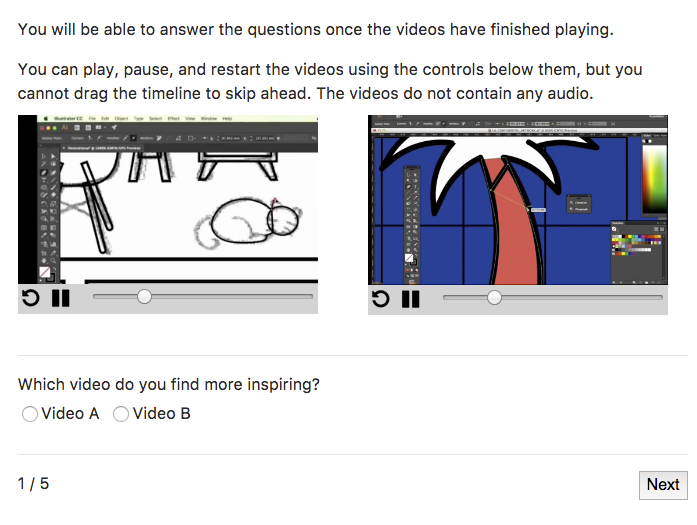
\includegraphics[width=\columnwidth]{liveclips/figures/mturk.png}
  \caption{An example of a pairwise comparison completed by Mechanical Turk workers. Each task involved five such pairs. In the introduction to the task, workers were asked to consider which 25-second video would inspire them to be more creative. }~\label{fig:liveclips_mturk}
\end{figure}

\section{Evaluation}
To evaluate whether our ranking metrics are effective at finding inspiring clips, we conducted a study on Amazon Mechanical Turk. This study did not evaluate clips in the context of creative software. Instead, it focused on whether timing and visual change are good general predictors for inspiring content. 

As described in the System section, RePlay generated 1,742 clips from our dataset of 30 hours of video of Photoshop and Illustrator use. We randomly sampled 129 of these clips to include in our evaluation set. To ensure we had coverage of all tools in our dataset, we randomly chose between 2 and 10 clips per tool. Since some tools are much more popular than others (e.g., Photoshop's brush tool had 939 clips whereas the burn tool only had 2 clips), this method allowed us to have a smaller sample while still representing every tool.

Workers compared video clips in pairs. Each Mechanical Turk task started with an overview page describing the task and showing an example pair of clips followed by five rounds of paired comparisons. Each comparison involved viewing two clips of the same tool and answering which clip they think would inspire them to be more creative (\autoref{fig:liveclips_mturk}). After completing all five comparisons, workers completed a short survey asking about their experience with Photoshop and Illustrator, and what types of creative tasks they do. Workers' results were only included if they completed all of the above steps. In an effort to ensure that they actually watched the videos, each comparison page only allowed workers to answer the question once both videos had played through once. Workers were paid \$1.50 per task, which took an average of 10 minutes and 20 seconds to complete. The same worker could do multiple tasks and would see five new pairs of videos (randomly selected) every time.

\subsection{Results}
In total, 481 workers completed 628 tasks, giving us a total of 3,140 paired comparisons. Most pairs were compared by 9 unique workers, though some ended up being compared more times. To balance results across clips, we considered only the first 9 comparisons for each pair. \autoref{table:experience} shows the distribution of workers' prior experience with Photoshop, Illustrator, and various types of creative tasks. Notably, 73\% and 35\% of participants had at least some experience using Photoshop and Illustrator respectively.

\begin{table}[b!]
\small
\centering
\begin{tabular}{lll}
            &                           & \# Participants \\ \hline
Photoshop   & None                      & 130 (27\%)       \\
experience  & Beginner                  & 242 (50\%)      \\
            & Intermediate              & 91 (19\%)       \\
            & Expert                    & 18 (4\%)        \\ \hline
Illustrator & None                      & 311 (65\%)      \\
experience  & Beginner                  & 114 (24\%)      \\
            & Intermediate              & 46 (9\%)       \\
            & Expert                    & 10 (2\%)        \\ \hline
Creative    & Physical drawing/painting & 247 (51\%)      \\
experience  & Digital drawing/painting  & 147 (31\%)      \\
            & Photography               & 386 (80\%)      \\
            & Photo editing             & 290 (60\%)      \\
            & Design                    & 144 (30\%)     
\end{tabular}
\caption{The distribution of workers' experience with Photoshop and Illustrator, and the types of creative tasks they have experience with.}
\label{table:experience}
\end{table}

Since only clips showing the same tool were compared, our analysis only examines ranking agreement within tool groups. Each tool group had between 2 and 10 video clips. For groups with only 2 clips, we determine the human ranking of these two clips by ranking whichever clip was chosen more often first, and the other second. For all other groups, we use the Bradley-Terry model as implemented in \cite{Maystre2015} to infer a ranking of clips within that group based on the paired comparisons. Within each group, we use Spearman's $\rho$ to compute the correlation between human rankings and RePlay rankings. RePlay rankings are based on the total score for each clip (time and visual change combined).

\textbf{Overall agreement between rankings ranges between very weak and moderate.} Since the groups have different sizes, we cannot compute one overall measure of correlation, as it is unclear what the null distribution would be. \autoref{table:agreement} (top) shows the average $\rho$ values for each group size. Note that $p$-values are not appropriate for such small group sizes, however the $\rho$ values still accurately represent the correlation between rankings. \autoref{fig:liveclips_agreement} (left) shows an aggregate comparison of all clip rankings. 

\textbf{Agreement between rankings for less-disputed clips ranges between weak and very strong.} The main goal of RePlay's ranking is not to establish an overall ranking of \textit{all} clips, but rather to ensure that bad clips are discarded, and that only the best clips are shown to the user. Therefore, any clips that had a large amount of disagreement between workers are likely not among the best. Indeed, if we restrict our selection of video clips to only those that either won or lost over 65\% of all comparisons they were a part of, this set consists of video clips that likely have a more obvious objective value. \autoref{table:agreement} (bottom) shows the average $\rho$ values for each group size when restricted to this smaller set of clips (in our sample set, 64/115). Overall we see stronger correlations. \autoref{fig:liveclips_agreement} (right) shows an aggregate comparison of all these clips' rankings; we see fewer large disagreements here than in \autoref{fig:liveclips_agreement} (left).

Timelapse clips did not perform significantly better or worse than standard clips. However, there were far fewer timelapse clips than standard ones in our dataset (19 vs. 96), due to the fact that longer sequences of a single tool use were less common overall than shorter sequences. A larger dataset is needed to determine whether or not timelapse videos may be preferred over standard ones.

\begin{figure}[b]
\centering
  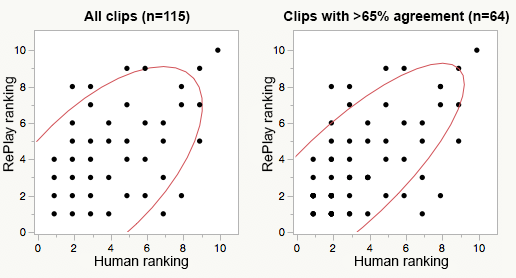
\includegraphics[width=\columnwidth]{liveclips/figures/agreement.png}
  \caption{Human ranking vs. RePlay ranking for all video clips (left), and all video clips with >65\% agreement among turkers (right). Note that there is more overall agreement between rankings in the subset on the right.}~\label{fig:liveclips_agreement}
\end{figure}

\begin{table}[b!]
\small
\centering
\textbf{All clips (n = 115)}
\vspace{5pt}
\begin{tabular}{l|llllllll}
\# Clips & 2    & 3 & 4 & 5   & 6    & 7    & 9    & 10   \\ \hline
\# Groups           & 18   & 5 & 2 & 1   & 1    & 1    & 2    & 2    \\
Mean $\rho$  & 0.11 & 0.3 & -0.2 & 0.6 & 0.09 & 0.54 & 0.21 & 0.48
\end{tabular}
\textbf{Clips with >65\% agreement (n = 64)}
\begin{tabular}{l|llll}
\# Clips & 2    & 3   & 4    & 5   \\ \hline
\# Groups           & 18   & 3   & 3    & 1   \\
Mean $\rho$  & 0.33 & 1.0 & 0.73 & 1.0
\end{tabular}
\caption{Average Spearman $\rho$ correlation between human ranking and RePlay ranking for all clips (top) and all clips with >65\% agreement among turkers (bottom), compared within each tool. ``\# Groups'' for column $i$ refers to the number of tools that have $i$ clips. Positive $\rho$ values indicate a positive correlation, with correlations above .2 considered weak, above .4 considered moderate, and above .6 considered strong.}
\label{table:agreement}
\end{table}

\section{Early user feedback}
The Mechanical Turk evaluation explored the viability of RePlay's ranking algorithm outside the context of an application. To get some initial user feedback on placing inspiring examples \textit{inside} an application, we recruited two casual Photoshop users, both male, to work on projects of their choice. They used Photoshop with all three interfaces enabled at once (on-demand search, ambient side panel, and contextual tooltips) (\autoref{fig:liveclips_photoshop}), and gave feedback while they worked.

Overall feedback was positive. Both participants found seeing video examples in the application useful and said that they wanted to see how others use tools and set parameters. The two participants differed in how they wanted to see examples. One participant preferred the tooltips, explaining that they were a nice level in between the on-demand search (which was easy to forget about) and the ambient panel (which they found distracting). They liked that if you happen to hover on a tool for an extra moment (which could happen by accident), it pops up and serves as a reminder that these examples exist, without taking away too much from the process. The other participant preferred the panel, and wanted to be able to refresh recommendations on demand and see a large variety of content. Both participants clicked on the videos and wanted to watch them in the browser where they could see them larger. 

This early user feedback is encouraging and shows the opportunity around embedding examples in the application.


\section{Discussion}

\subsection{Can we really predict what will be inspiring?}
The results from the ranking evaluation presented in the previous section should be taken with a grain of salt. The workers who participated in this study were not all users of creative software, and the video clips were presented out of context. The evaluation was intended as an initial baseline to determine whether RePlay's ranking algorithm can reasonably identify good clips. The subjective nature of the question workers were asked meant that we could not include a ``ground truth'' comparison to filter out lazy turkers. We did however enforce that the entire video clips played at least once before workers could select an answer.

Aside from the questions that using crowd-worker participants raises, the idea of ``inspiration'' is subjective and hard to predict. What one person finds inspiring another may not. Whether someone finds something inspiring could even change depending on the time at which they see it. Despite these challenges, we had reasonable agreement among workers overall; the average percent of agreement across all pairs of clips was 74\%, (SD 14.5). Even if Mechanical Turk workers \textit{were} a 100\% reliable source, we would still expect some disagreement, due to the subjective nature of the question.

The RePlay algorithm can reasonably identify clips that most workers agree are either good or bad. It is important to keep in mind that the main purpose for this algorithm is to address the ``cold start'' problem. Once people start using an interface with video examples, RePlay could continually improve the ranking algorithm based on user behaviour and preferences, exhibited through how much people interact with the videos. %There are other low-level features of clips identified by Lafreniere et al. \cite{Lafreniere2014} that could also be included in a ranking algorithm, such as whether a clip shows parameters being set, but we chose not to include these in the RePlay algorithm because it is likely that the \textit{content} of a video's artwork will be the main factor that determines its inspirational value. but this is a hard problem.

\subsection{How diverse should the set of examples be?}
Research on examples and creativity is rather divided regarding whether diverse examples that are distantly related to the user's task are better than a narrow set of examples that are more closely related to the user's task. Some work has shown that more diverse, far-off examples improve creativity by encouraging people to think more broadly and try new things \cite{Chan2011, Siangliulue2015a}, while other work has shown that similar examples are more useful as they are more relevant to the user \cite{Chan2015}. More recently, Benjamin et al. \cite{Benjamin2014} propose letting the user decide by providing an adjustable slider that determines the diversity of recommended examples, based on the idea that the need for more diverse or more similar examples may differ depending on where the user is in their process.

Another option could be to let users search by example, a feature that is now common in search engines. Rather than having to specify an exact query, users could provide an example video and ask for ``more like this''. However even in this case the diversity of results is an important factor to consider.

%let's cut this for now.It's good but not as connected to inspiration as the the previous sections, which work well together
%\subsection{How much information should recommendations show?}
%Prior research has shown the benefits of being transparent with users about how recommendations are chosen \cite{}. In our three interfaces, contextual tooltips are transparent by nature, as they show only clips of the selected tool. However the method for choosing clips in the search window and panel is currently rather opaque. It may be helpful to provide users with more detail regarding why a clip was chosen, for example because they used a certain tool recently. 

%More generally, providing users with enough information scent to make a quick but informed decision about whether they should give their attention to an example is important. This highlights a challenging trade-off in the design of contextual interfaces: showing users enough information without making it too costly to review this information \cite{?}. While there are many additional things that could be shown along with a video clip (a description of it, the audio transcript, the tools used in it, an overview of the task it shows, etc.) and existing methods for highlighting important activity within the clip (highlighting mouse movement or areas of change \cite{}, showing what keys are being pressed when \cite{}), incorporating all of this information would quickly become overwhelming. Prior work has shown that a brief text description can help users efficiently scan a set of video clips \cite{}; this may be a good starting point.
\section{Limitations \& Future Work}
This chapter presented initial work exploring ways to bring inspiring examples into the creative process, and a new type of content from which to draw such examples: creative live stream videos. We provide suggestive results that our algorithm can select potentially inspiring clips, and some initial user feedback on our prototype interfaces indicating that this is a promising avenue for future work. Rather than conduct a rigorous controlled study (which is difficult and often inappropriate for evaluating goals like creativity and inspiration \cite{Shneiderman2007}), this chapter aims to introduce this space and lay out the possibilities for future work to explore. In this section, we discuss a few main directions for such work.

\subsection{More Robust Segmentation and Change Ranking}
Our current methods for detecting visual change use simple computer vision approaches, and exhibited some failure cases. We have yet to try more sophisticated deep learning methods to segment this data but this is a promising direction of future work that could help improve the classification of panning, zooming, and parameter setting. Having more robust and available usage data could also improve the detection of such features. For example, Lafreniere \textit{et al.} \cite{Lafreniere2014} used instrumented software to gather both videos and detailed usage, which allowed them to calculate visual change directly by counting the number of pixels on the artist's document that change during a video clip. As of recently, streamers on Behance (\href{https://behance.net/live}{\nolinkurl{behance.net/live}}) can use a plugin that logs their command usage while they stream in creative software. This data can be used to segment live stream archives \cite{Fraser2020}, but such segmentations would still benefit from logs or analysis of visual and spatial information.

In addition, to make use of the large amount of video content that already exists online with no available telemetry, a deep learning system could be trained on those videos that do have usage data, and then applied to videos that do not.

\subsection{Making Use of Audio and Chat Logs}
Live streamed videos come with additional data that this work did not make use of: audio in the form of the streamer's narration and responses to questions (which can be transcribed to text) and chat logs from viewers of the stream. Making use of audio narration in software tutorial videos is an open problem \cite{Chi2012} as narrations don't always align exactly with the artist's actions. Live streamed videos have a similar problem that is exacerbated by the fact that artists are not always narrating what they are doing; sometimes they are answering questions from the chat and other times they are simply talking about unrelated things as they work. Future work should explore ways to detect when those different types of narration are occurring, and make use of their content as appropriate, for example highlighting moments where artists answer questions, or building a mapping of ways in which artists describe their software actions in natural language.

Chat logs can also be a useful data source to include in future work. Though the content of live chats tends to be very noisy, especially on popular channels \cite{Hamilton2014}, the frequency of chat posts at a given time can indicate exciting or interesting moments \cite{Pan2016}. Chat post frequency could therefore be used as another criteria for ranking clips.

\subsection{Other Ways to Generate Short Clips from Long Videos}
This work focused on generating tool-based clips, inspired by prior work \cite{Grossman2010a, Lafreniere2014} and the natural mapping between tool use and user behaviour. However, while tool-focused clips are good for showing users how a tool works \cite{Grossman2010a}, they may not be the most inspirational types of clips one can generate from long videos. Other methods could include breaking videos into higher level sub-tasks (based on pauses in tool activity and narration content), or extracting clips where the artist describes a particular technique or answers a question. As one of the exciting parts of watching a live stream is seeing an artist go from a blank canvas to a finished work, another option could be to shorten the entire video down to a short summary. This could be done by removing sections where the artist takes pauses, talks with no actions, and switches applications; and by adapting existing techniques for creating short video summaries from long videos (\textit{e.g.}, \cite{Truong2007}). 

\section{Conclusion}
This chapter explored a growing form of creative videos very different from traditional tutorials: live streams. We found that creative live streams are a good source of both learning and inspiration, and introduced an approach for bringing inspiration into the context of creative software users' workflows. 

RePlay, ReMap, and LiveClips all leveraged \textbf{visual media} in the form of screencast videos for providing contextual support towards understanding creative processes. But for users who just want to get a task done without spending time on the individual steps required, videos can be too tedious and detailed. The next two chapters explore how two different types of resource -- \textbf{executable code} and \textbf{written text} -- can help people quickly and easily achieve creative outcomes.


\section{Acknowledgements}
We thank Tricia Ngoon, Kandarp Khandwala, and Nicolas La-polla for their help with live stream analysis, and our study participants for their insights. This work was supported in part by NSERC, Adobe Research, and NSF award \#1735234.

This chapter, in part, includes portions of material as it appears in \textit{Sharing the Studio: How Creative Livestreaming can Inspire, Educate, and Engage} by C. Ailie Fraser, Joy O. Kim, Alison Thornsberry, Scott Klemmer, and Mira Dontcheva in the Proceedings of the 2019 on Creativity and Cognition (C\&C '19). The dissertation author was the primary investigator and author of this paper.

This chapter, in part, includes portions of material coauthored with Andy Edmonds and Mira Dontcheva. The dissertation author was the primary investigator and author of this material.

\chapter{RePlay: Contextually Presenting Learning Videos Across Software Applications}
\label{chapter:replay}
\begin{quote}
Complex activities often require people to work across multiple software applications. However, people frequently lack valuable knowledge about at least one application, especially as software changes and new software emerges. These gaps in knowledge often arise while people are in the middle of the task, leading them to search for help. Unfortunately, existing help systems either lack contextual knowledge or are tightly-knit into a single application. We introduce an application-independent approach for contextually presenting video learning resources and demonstrate it through the \textit{RePlay} system. RePlay uses accessibility \textsc{api}s to gather context about the user's activity. It leverages an existing search engine to present relevant videos and highlights key segments within them using video captions. We report on a week-long field study ($n\!=\!7$) and a lab study ($n\!=\!24$) showing that contextual assistance helps people spend less time away from their task than web video search and replaces current video navigation strategies. Our findings highlight challenges with representing and using context across applications.
\end{quote}

\begin{figure}[b!]
\centering
  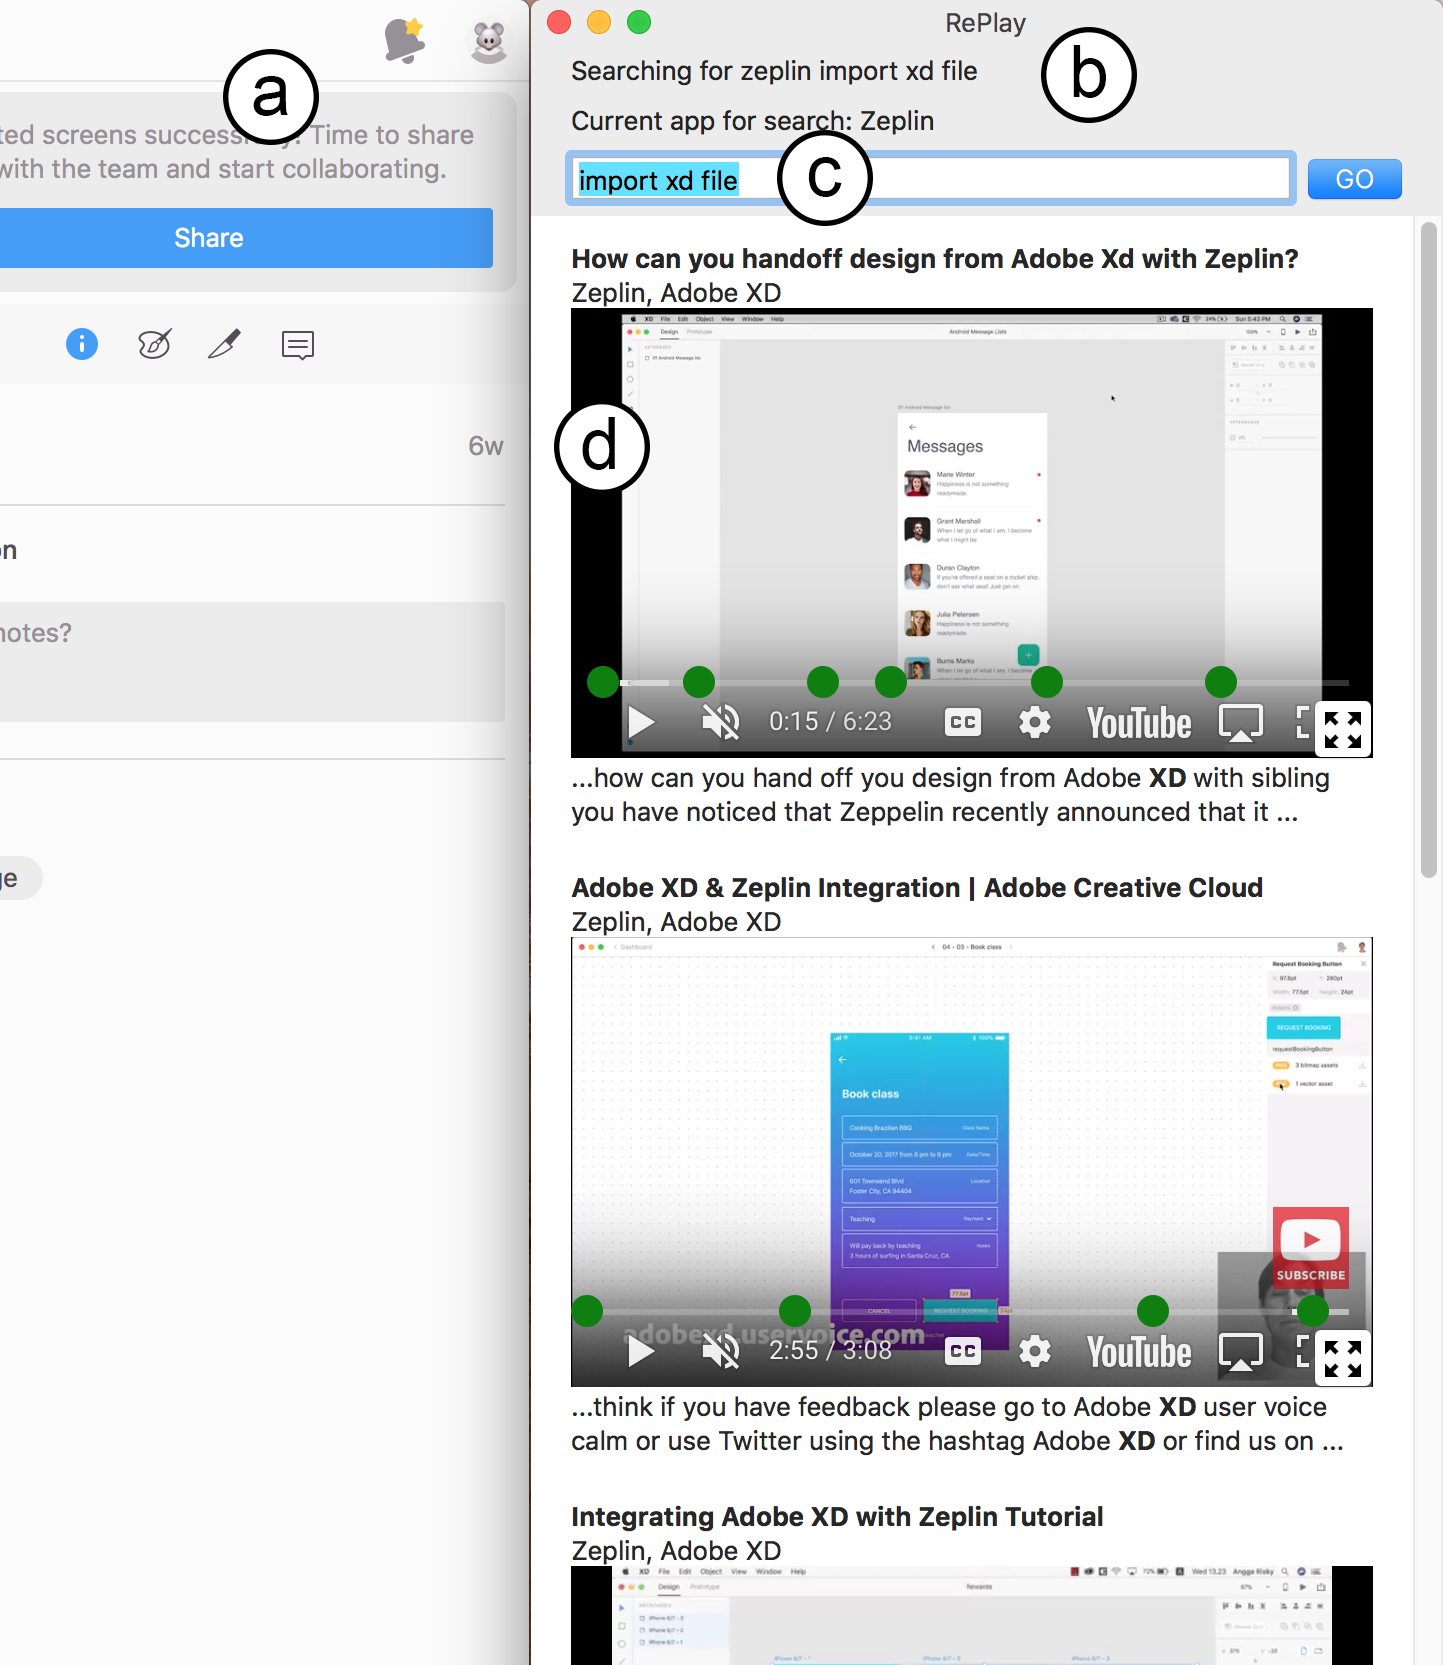
\includegraphics[width=0.7\textwidth]{replay/figures/replay-interface.png}
  \caption{RePlay - shown to the right of Zeplin (a) - includes a status area (b) and search field (c) at the top. Video results (d) include timeline markers and caption excerpts to highlight moments relevant to the user's query and context.}
  \label{fig:replay-interface}
%   \Description[A screenshot of RePlay's interface next to the application Zeplin.]{A screenshot of RePlay's interface next to the application Zeplin. RePlay comprises a status area, a search field, and video results. Timeline markers and caption excerpts overlaid on video results highlight moments relevant to the user's query and context.}
\end{figure}

\section{Introduction}
Most software activities span multiple applications. The slogan ``there's an app for that'' illustrates that we live in a world filled with specialized apps that each focus on a few specific tasks. To accomplish larger activities requires composing multiple applications together into a ``toolbelt'' \cite{Sumner1997}. For example, designing an interface might comprise drawing a logo in Illustrator, mocking up a prototype in Sketch, adding animations using Flinto, and presenting it to a client using Keynote. Analyzing data might involve formatting it using Python, viewing and graphing it in Excel, modifying graph aesthetics in Photoshop, and reporting results in Word. Toolbelts help users tailor custom ecosystems and support distributed innovation. However, this bricolage creates a user experience problem: even with design guidelines, every application is different \cite{Beaudouin-Lafon2018}. As new applications appear and existing ones change, few people are fluent experts in all the steps towards their goals.

Presenting learning resources in-application \cite{Grossman2010a, Chilana2012, Matejka2011a, Matejka2011, Brandt2010, Ichinco2017} and augmenting search queries with contextual information \cite{Ekstrand2011, Brandt2010} can offer a more fluid experience with lower cognitive load. However, existing solutions require deep integration with applications. And since today's applications are ``walled gardens''  with limited integration across software vendors \cite{Beaudouin-Lafon2018}, help resources typically focus on one application at a time. This leaves gaps when users want to move from one application to another (\textit{e.g.,} export an Adobe \textsc{xd} prototype to Zeplin) or interleave applications (\textit{e.g.,} coding a website in Sublime while debugging in Chrome and resizing graphics in \textsc{gimp}). 

% Web search results can of course include community-created resources that span applications. However, generic web search poses two problems. First, search is blind to relevant contextual information that could connect users to better resources \cite{Ekstrand2011, Kraft2005, Finkelstein2002}. Search engines place the burden on users to articulate an appropriate query, an almost paradoxical requirement for users who are there because they don't know the domain \cite{Russell2011}.  Second, search is divorced from the application UX, requiring users to bounce back and forth to connect the content \cite{Fourney2014Intertwine}. These challenges are amplified when users work with multiple applications, each with its own terminology and conventions.

We introduce an application-independent approach for contextually presenting video learning resources. We embody this approach in the RePlay system (\autoref{fig:replay-interface}), which enables users to search for learning videos based on their application usage. RePlay gathers application context using system accessibility \textsc{api}s. It extends online video search and cues videos to relevant segments based on their captions. We focus on video assistance because despite video's growing popularity (Cisco predicts that by 2021, 82\% of all internet traffic will be video \cite{Cisco}), searching and browsing videos remain cumbersome \cite{Kim2014, Pavel2014, Pavel2015}. Video is popular for content creators as it is often easier to author than tutorials or diagrams (which require careful curation). Learners value video for its efficacy in communicating complex or continuous visual actions such as brushing or setting parameters \cite{Chi2012}. However, interacting with videos remains difficult because they are harder to navigate and scan for steps than text \cite{Chi2012}.

%for its popularity as a learning resource \cite{Chi2012, Pongnumkul2011, Nguyen2015}, especially for visual tasks
%its simultaneously the most useful thing for many tasks and also the least well supported by current search interfaces
% while video has become increasingly ubiquitous and easy to create -- ... -- searching and browsing remain cumbersome.

We report on two studies observing how people use RePlay and web video help: a week-long field study ($n\!=\!7$) and a lab study ($n\!=\!24$) where half the participants used RePlay and half used web video search. Both studies used visual design as the domain, as video is especially helpful for visual tasks \cite{Pongnumkul2011}. The field study examined how designers with varying experience used RePlay in-situ. Participants used an average of 17 different applications in a week, emphasizing the importance of system-wide integration. Our findings also suggested that contextual video assistance benefits targeted tasks more than open-ended ones. The lab study found that contextual video assistance helps people spend less time away from their task than web video search, and replaces strategies typically used in navigating between and within videos. This work makes the following contributions:

\begin{enumerate}
    \item An application-independent method for finding relevant clips in learning videos that leverages user context,
    \item the RePlay system, which demonstrates this method using accessibility \textsc{api}s and online video corpora, and
    \item insights from two studies that highlight the importance of multi-application support and the promise of cross-application search.
\end{enumerate}




% replay is an example implementation of such a tool / embodiment of this approach / design probe to illustrate how this could be done, and investigate whether it helps people. / show that this is a viable direction for future research 

% people dream of this thing. we offer a new path to achieve aspects of that goal. knitting help together lowers the friction between applications

% arg 1: lack of integration creates friction that our work mitigates
% ****arg 2: if you need to assemble a buncha tools that all work differnetly you won't know them all
% arg 3: the seams / hand off points require guidance

%Currently, it is difficult for users to get effective guidance when tasks span applications: in-situ help and official documentation is only available at the individual application level, and community-created resources that sometimes do span applications move the user out of their workflow and into the browser. 


%include Google YT timeline marker result as an example
%have IoT example for camera-ready video
% somewhere also mention accessibility for all argument

%watching ppl use 2 different video interfaces taught us what a good video interface should be (wouldn't be able to find this otherwise)

\section{Related Work}
%YouTube also contains many videos that specifically address cross-app workflows (e.g., exporting content from one application and importing it into another). 
This work builds on prior contextual search and video segmentation work with a novel focus on multi-app activities.
%This necessitates an application-general approach for detecting context and a domain-general approach for searching and ranking. 

\subsection{Multi-app activities are hard to support consistently}
People often work across multiple applications that each support an individual task to perform higher-level activities \cite{Sumner1997}. Help systems for such applications tend to focus on their individual tasks rather than the transitions and interactions between them \cite{Norman2005}. Implementing system-wide assistance that captures activity context is difficult, as every application has its own conventions and interface, and software interoperability tends to be limited \cite{Beaudouin-Lafon2018}. Accessibility \textsc{api}s are one useful entry point for diverse system-wide extensibility, including visualizing user behavior \cite{Matejka2013}, voice control \cite{Li2017, Zhong2014}, and modifying or enhancing existing user interfaces \cite{Dixon2014, Stuerzlinger2006, Chang2011}.
RePlay uses accessibility \textsc{api}s for detecting system-wide application context.
% one inspiration for this work is the emergence of creative professionals live streaming their work. these live streams offer a more holistic view than ``help'' because viewers can see how specific functions fit together. 

\subsection{Application context improves relevance and presentation of learning content}
The most teachable moment for software tasks is often when the user is actively working... but stuck. In-task help for a specific goal is one of the biggest reasons people seek web \cite{Lafreniere2013a} and video \cite{AlamAnik2015} tutorials. However, tutorials tend to show a full task from start to finish, much of which may not be relevant to the user's current goal. This leaves it to the user to both find a relevant tutorial and locate the segment(s) within it that contains the needed information.

Effectively searching the Web is an acquired skill; coming up with the right keywords and search settings can be difficult, especially for novices \cite{Russell2011}. In addition, web search environments lack context that human tutors use to proactively offer help and tailor feedback \cite{Schon1983}. Adding contextual terms automatically to search queries (\textit{e.g.,} \textsc{os} version, application, recently-used tools) can help improve the relevance and utility of search results without requiring the user to know app-specific terminology \cite{Ekstrand2011, Brandt2010, Matejka2011a}. RePlay augments queries with the current application name and uses context from both the current and recently-used applications to support cross-app activities when ranking search results.

Adding contextual cues to search results provides information scent that can help users more quickly and easily navigate the results (\autoref{fig:replay-green_markers}). Such cues show how and why a result is relevant to the user's own situation and direct them to the relevant information within a result \cite{Ekstrand2011, Fourney2014Intertwine}. RePlay expands these ideas to video, displaying contextual cues for recently-used applications and tools.

Bringing learning resources directly into applications reduces the need for context switching. For example, proactively recommending content in-situ based on user context can lead users to resources they might not have even thought to search for \cite{Matejka2009, Fraser2016, Chilana2012, Matejka2011, Ichinco2017}. In-app search also helps users stay focused on their task while learning \cite{Lafreniere2014a, Fraser2016, Chilana2012}. RePlay brings these strategies into an application-independent system, functioning alongside the user's applications.

\subsection{Videos are helpful for learning but hard to navigate}
Videos are popular for many kinds of tasks, especially visual ones, because they show clear demonstrations that might be harder to explain or understand in text \cite{Chi2012, Pongnumkul2011}. Videos are widely available and relatively easy to make. Software is always being updated, and new video demonstrations are constantly added to popular platforms by the user community to keep up with updates and current trends. However, while text-based documents are easy to skim and search, videos are not \cite{Pavel2014, Pavel2015, Kim2014}. The predominant video search approach displays results as thumbnail images with a title and summary (\textit{e.g.,} YouTube, Vimeo). This presentation only provides a broad overview without cues about matching content; prior work has shown that people look for indications of how search results are relevant to their query \cite{Hearst2009Book}. Navigating within videos is typically limited to hovering across the timeline with a small visual preview.

Automatically dividing videos into conceptual chunks can improve peoples' ability to find useful information for their task \cite{Pongnumkul2011, Chi2012, Banovic2012, Nguyen2015, Grossman2010a, Matejka2011}. RePlay uses captions to select relevant clips \cite{Pavel2014, Pavel2015, Girgensohn2005}. Automatic clip selection plays a limited but growing role in web search. Google displays a ``suggested video clip'' \cite{Sullivan2018} as the automated summary for some searches, and Bing's ``smart motion preview'' feature \cite{Bing} shows a 30-second preview for video search results. In contrast, RePlay focuses on searching with and presenting results within application context. Chi et al. \cite{Chi2012} showed people benefit most from a mix of text and video; RePlay combines video and text instruction by presenting captions with videos for both navigational and learning assistance.

Methods for navigating between video segments include interactive timeline markers \cite{Matejka2011, Grossman2010, Kim2014, Banovic2012, Kim2014a}, thumbnail images \cite{Kim2014a, Pongnumkul2011, Banovic2012, Grossman2010a, Chi2012, Pavel2014}, transcript text \cite{Kim2014a}, and clickable elements overlaid on the video \cite{Nguyen2015}. Like Ambient Help \cite{Matejka2011}, ToolScape \cite{Kim2014}, and Chronicle \cite{Grossman2010}, RePlay overlays markers on the timeline indicating command or tool use. We use timeline markers over other options as they take up little space and allow for pop-up text previews, which aid browsing. While prior work marks \textit{all} instances of tool use or interface actions, RePlay marks only \textit{contextually-relevant} moments (recently-used tools and words from the user's query) to reduce clutter and unnecessary detail in a small interface.


%As a result, the learning materials online differ for each application as well. Different keywords may be necessary to find help for a given task depending what application you are using for that task.
%But maybe we don't need application-specific knowledge. Maybe we can just make use of existing system-wide functionality, get the minimum information it provides for most applications, and use that to augment existing search engines just enough to support these activities a little better.

%This requires the user to translate their own context and situation back and forth with that in the browser. Users must determine what of their context might potentially be relevant and articulate a search query appropriately, determine which search results might be relevant to this context based on their information scent, and finally map the instructions received back to their own unique situation. (maybe move to a separate section?)
\section{RePlay System}
This section describes RePlay's user interface, context detection, and system architecture.
%RePlay is a desktop application that allows users to search for contextually-relevant video clips for any accessibility-enabled desktop application. It leverages large online video corpora, searching video caption text for relevant moments. The RePlay prototype investigates the efficacy and challenges of cross-app contextual search.

\begin{figure}[b!]
\centering
\vspace{-0.2in}
  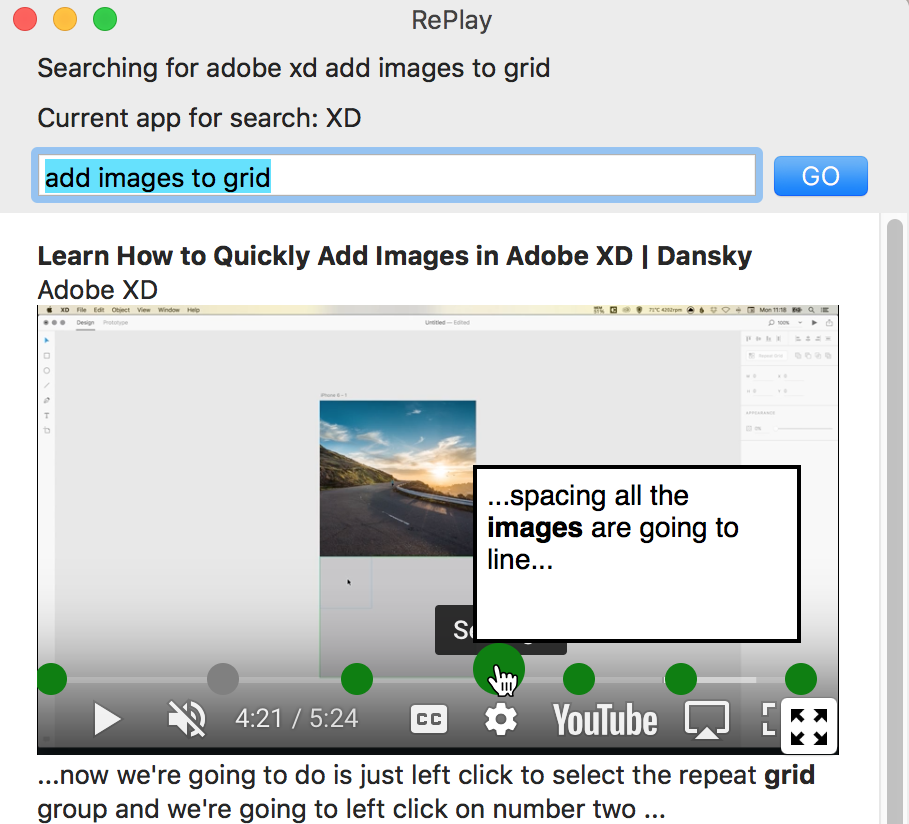
\includegraphics[width=\textwidth]{replay/figures/green_markers.png}
  \caption{RePlay overlays green markers on the video timeline to indicate moments where the captions match a user's search term. Mousing over a marker shows a pop-up with an excerpt from the captions at that moment; clicking it plays the video from that moment. }~\label{fig:replay-green_markers}
%   \Description[A screenshot showing green markers overlaid on a video result in RePlay.]{A screenshot showing green markers overlaid on a video result in RePlay. The user has searched for ``add images to grid'' in Adobe XD, and the top video result is titled ``Learn how to quickly add images in Adobe XD''. The video timeline has green dots on it, and the mouse is hovering over one. A pop-up shows a caption excerpt that says: ``...spacing all the images are going to line...'' with the word ``images'' bolded.}
  \vspace{-0.2in}
\end{figure}

\subsection{User interface}
The RePlay panel (\autoref{fig:replay-interface}) can be positioned and sized as desired; its default size is 465px \texttimes 1055px. It is designed to fit next to the user's primary applications to minimize switching windows. The narrow pane makes videos small but easier to browse and watch in context. The interface comprises a status area, search field, and video results.

The status area updates as the user works, displaying the name of the last tool clicked and the current application (\autoref{fig:replay-status}). ``Tools'' refer to interface elements or commands within an application. The status area provides awareness of what context RePlay will use for search (\textit{i.e.,} so the user does not need to include the application name in their search query). When the user initiates a search, the status area updates to show the query (\autoref{fig:replay-interface}b).

As the user works, the search field updates with the name of the last tool clicked (\autoref{fig:replay-status}). Users can edit or delete it to form their own query. Pressing the \textsc{go} button or return key triggers a search. RePlay displays the top five resulting videos, each cued to start at a relevant moment. A two-line excerpt from that moment's caption appears below the video with query words highlighted in bold \cite{Hearst2009}.

Often, videos have multiple moments that may be relevant. RePlay renders green markers on the video timeline to indicate these moments. Mousing over a marker invokes a pop-up text area displaying a caption excerpt with words from the query in bold (\autoref{fig:replay-green_markers}). This pop-up obscures YouTube's default thumbnail pop-up but provides more useful information, as software videos tend to show an entire screen and shrinking this to a thumbnail makes it hard to see. Clicking a marker starts the video from that moment. 

\begin{figure}[b!]
\centering
\vspace{-0.2in}
  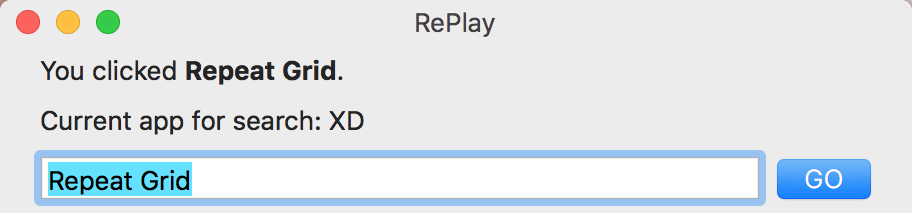
\includegraphics[width=\textwidth]{replay/figures/replay_status.png}
  \caption{RePlay's status area displays tool names after they are clicked and adds them to the search field. }~\label{fig:replay-status}
%   \Description[A screenshot of RePlay's status area.]{A screenshot of RePlay's status area. It reads, ``you clicked Repeat Grid'', and has the tool name ``Repeat Grid'' included in the search field.}
  \vspace{-0.2in}
\end{figure}


RePlay also displays contextual cues \cite{Ekstrand2011} on search results (\autoref{fig:replay-context_cues}). For each video, RePlay lists the three most-recently used applications that are mentioned in the video (\autoref{fig:replay-context_cues}a). This list is especially useful when users move between applications and want videos that mention both the current and recent applications. RePlay renders grey timeline markers to indicate moments where recently used tools are mentioned (\autoref{fig:replay-context_cues}b). Caption pop-ups italicize tool names.


\begin{figure}[b!]
\centering
\vspace{-0.2in}
  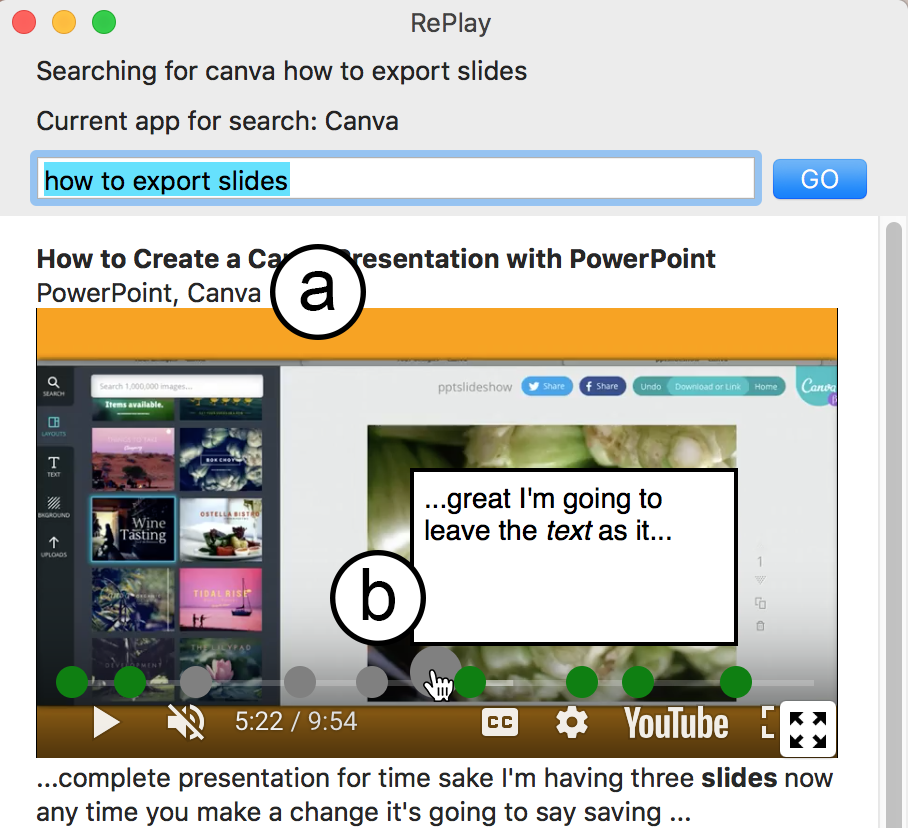
\includegraphics[width=\textwidth]{replay/figures/context_cues.png}
  \caption{RePlay displays contextual cues based on recent app and tool use. a) RePlay lists the three most recent apps that the video mentions. b) Grey markers indicate mentions of recently-used tools. In this example, the user recently used the ``text'' tool in Canva. Mousing over a marker shows a caption excerpt; clicking a marker plays the video. }~\label{fig:replay-context_cues}
%   \Description[A screenshot showing grey markers overlaid on a video result in RePlay.]{A screenshot showing grey markers overlaid on a video result in RePlay. The user has searched for ``how to export slides'' in Canva, and the top video result is titled ``How to create a canva presentation with PowerPoint''. The video timeline has grey dots on it, and the mouse is hovering over one. A pop-up shows a caption excerpt that says: ``...great I'm going to leave the text as it...'' with the word ``text'' italicized.}
  \vspace{-0.2in}
\end{figure}

RePlay's panel shows all results at the same time, allowing users to quickly skim multiple videos, and browse other results while one video plays. This ability to ``see inside'' multiple resources from a single page increases foraging efficiency \cite{Vermette2017, Glassman2016, Pavel2013}. 

Clicking the full-screen button in a video's bottom-right corner opens the video in a separate window that stays above all other windows while it is open, so that users can watch a video at a larger size when desired.

When the user switches to a new application and clicks a tool, RePlay automatically searches for the application name. This seeds the panel with app-relevant videos that give users a starting point.

\subsection{Detecting application context}
RePlay uses contextual information to augment a user's query and search within video results. The motivation for context-augmented search is to increase relevance, especially when users don't know what to ask for. However, if not done well, adding terms has the opposite effect: excluding relevant results and/or presenting irrelevant ones \cite{Finkelstein2002}. We tried several heuristics with RePlay; the current implementation includes the three most recent applications and tools.

\subsubsection{How to detect context?}
RePlay leverages \textsc{os} accessibility \textsc{api}s to detect every click. On each click event, RePlay retrieves the name of the click's source application, the type of element clicked, and the element's accessibility description (when present). If the element is a button, checkbox, text field, slider, or menu item, RePlay stores it as a recent tool and updates the status area and search field with the tool's name. If the user switched applications since their last click, RePlay updates its status area to reflect the new application, and resets its list of recent tools.

\subsubsection{Challenges with detecting context via accessibility}
Extracting accessibility text obviates the need for hard-coded knowledge about specific applications. The challenge of this system-wide approach is that despite platform accessibility guidelines, applications vary widely in what accessibility they offer and how \cite{Hurst2010}.

In Mac\-OS, RePlay can always extract the application name and menu items. Buttons and other interface elements have accessibility labels in many applications (\textit{e.g.,} Adobe \textsc{xd}, Microsoft Office, iMovie, Tableau, Sketch), but not in others (often long-existing software, \textit{e.g.,} Photoshop). Applications differ in which accessibility fields they support and what information is in what field. For example, tool names may be in the \textit{Title}, \textit{Help}, \textit{Description}, or \textit{Value} attribute. RePlay checks all four, preferring them in that order. RePlay also gathers accessibility information for websites, as long as browser accessibility access is enabled. It is by default in Safari, and as an option in Chrome. Many sites implement accessibility labels (\textit{e.g., } Canva, Wordpress, Sketchpad, Snappa, G Suite). Those that do not still include some information by default (\textit{e.g.}, text area contents via the \textit{Value} attribute). RePlay infers website names from the \textsc{url} and website title.

\subsection{Video search \& ranking}
RePlay leverages existing online video search engines to retrieve video results. It then finds and ranks relevant clips within these videos (\autoref{fig:replay-system}). RePlay's architecture requires no prior understanding of the applications or videos; it relies on captions for clip extraction and ranking. Video authors often talk about things they are doing and provide tips about tools; captions thus provide narrative information beyond the visual content in the video that can be useful for learners.

\begin{figure}[b!]
\centering
\vspace{-0.2in}
  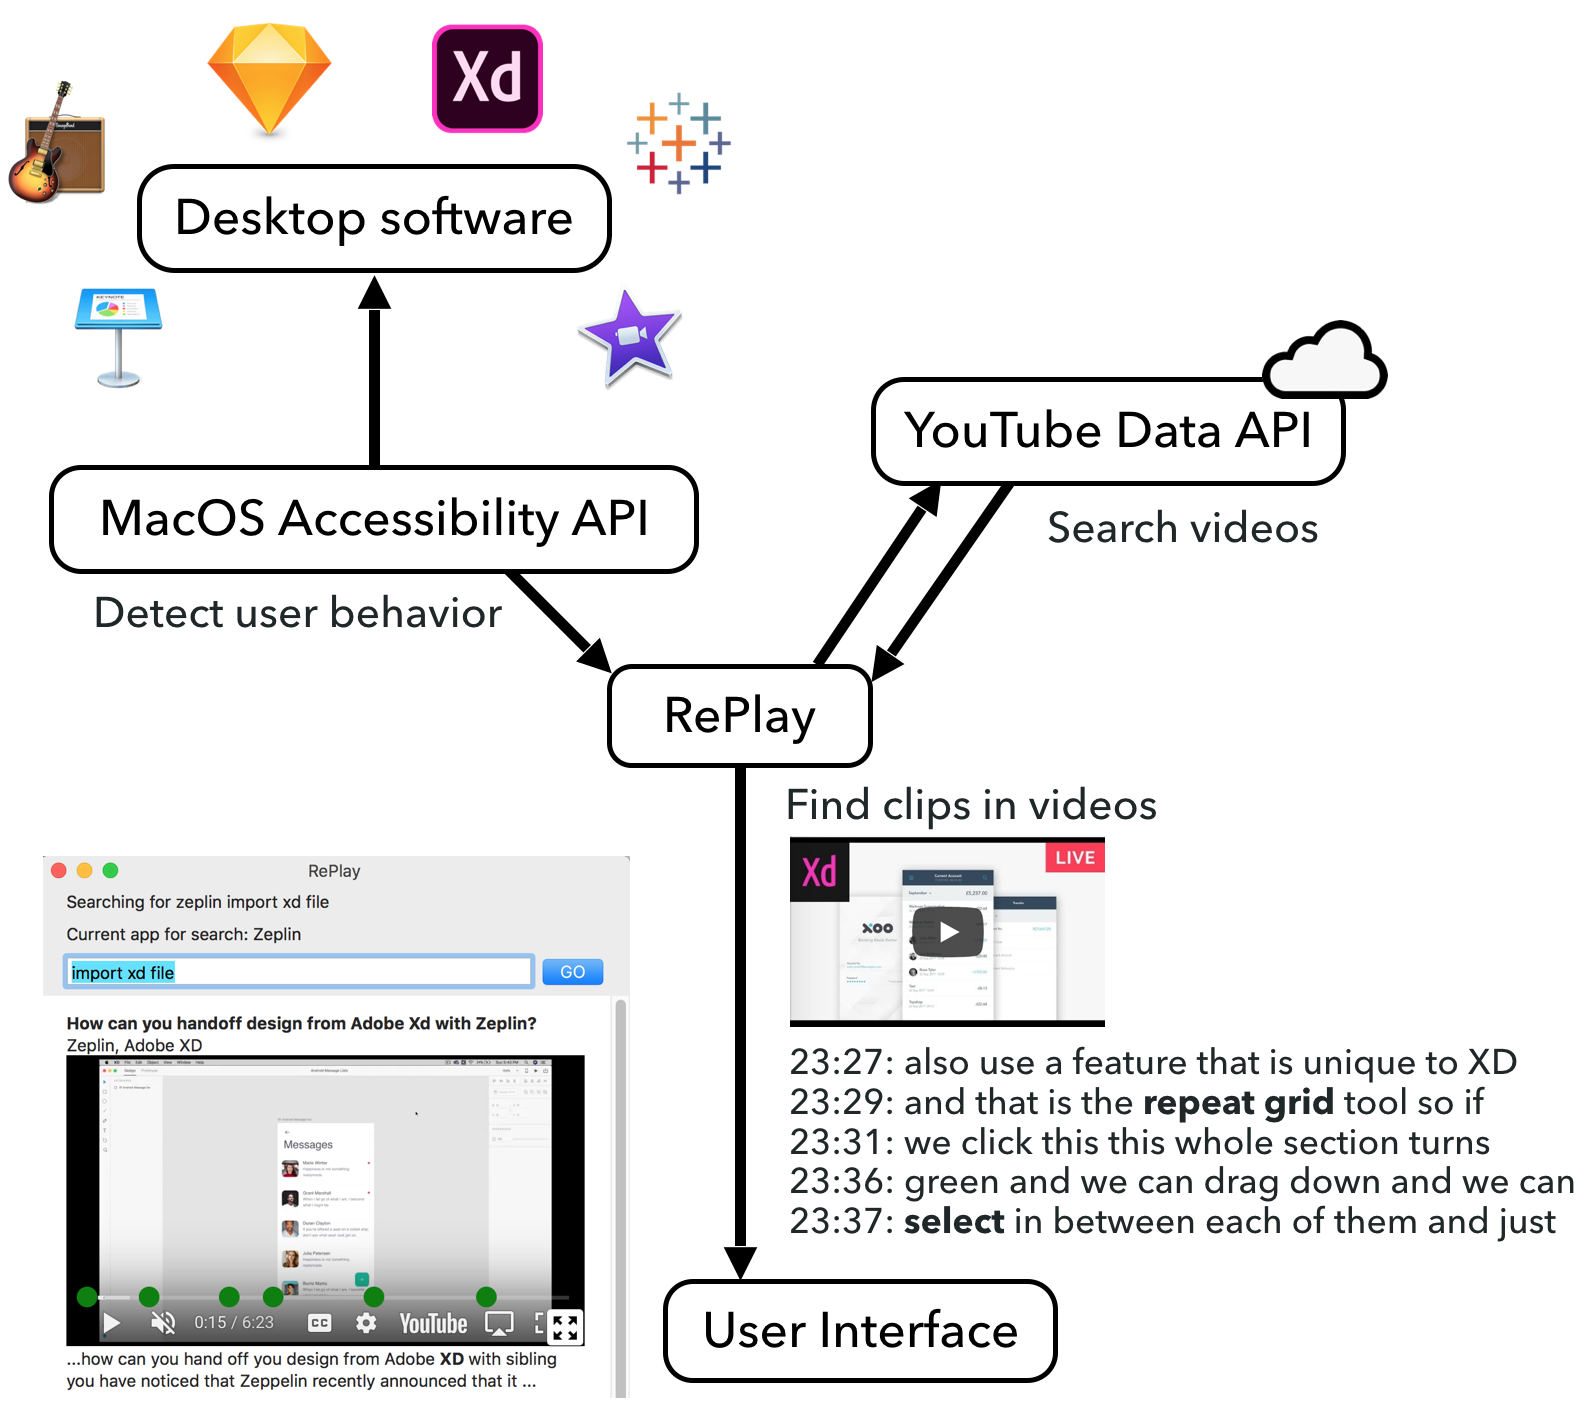
\includegraphics[width=\textwidth]{replay/figures/replay-system.png}
  \caption{RePlay uses accessibility \textsc{api}s to detect user context, which it uses to augment the user's query and to search and rank videos. RePlay finds matching clips by searching video captions for the user's query and recent tool names. }~\label{fig:replay-system}
%   \Description[A diagram showing the different components of RePlay and how they communicate.]{A diagram showing the different components of RePlay and how they communicate. The MacOS Accessibility API detects user behavior from desktop software and sends this to RePlay. RePlay searches videos using the YouTube Data API. RePlay finds clips in these videos and displays them in the user interface.}
  \vspace{-0.2in}
\end{figure}

\subsubsection{Available data}
RePlay's current video corpus comprises all English videos on YouTube that have a caption track. Most do: YouTube auto-generates captions by default. We used YouTube for its popularity and captions; any video search engine with an \textsc{api} could be used. For example, Vimeo (\url{vimeo.com}) and Dailymotion (\url{dailymotion.com}) also provide \textsc{api} access to videos and captions.

\subsubsection{Searching}
Video search requires more steps than document search, because captions are obtained separately. This two-step search means that issuing multiple queries with context terms added (such as tool usage) like prior work \cite{Ekstrand2011} would be too slow. To speed responses, RePlay constructs and issues a single query concatenating the current application's name with the user's query. Leaving context terms out of the query also ensures that the user-provided search terms are not ``washed out''. RePlay queries YouTube and selects its top five video results that have English captions and mention the current application in any of the title, description, or captions (to avoid results that may contain other keywords but do not pertain to the current application).

\subsubsection{Finding clips and re-ranking videos}
Several techniques automatically extract instructional video clips from screencasts of software use. The dominant approach leverages application usage \cite{Grossman2010, Lafreniere2014, Chi2012, Wang2018}, requiring that the video be recorded in an instrumented version of the software. Alternatively, computer vision can detect tool-selection events \cite{Pongnumkul2011, Matejka2011}, even without prior knowledge about the specific software \cite{Banovic2012}. To be application-independent and embed online videos directly without waiting to download and process them, RePlay instead uses metadata and caption text to rank and segment videos. 

For each video result, RePlay divides its captions into 30-second segments, searching each for the queried keywords (with stop words removed) and names of the three most-recently used tools in the current application. It ranks all segments by the total number of keyword matches. To break ties it uses number of tool name matches. The highest-ranked segment determines the video's start time. Timeline markers denote the top ten segments: green for those with a query term; grey if only a tool is mentioned. RePlay re-orders the video results based on the total number of matching clips. To break ties it uses the total number of matching keywords within the clips.

Although automatic captions are far from perfect, we found them to be sufficient for searching in RePlay. Captions are already an approximation of what the demonstrator is doing, so despite some errors, they work well enough for identifying potentially relevant moments. Having any aids for navigating within videos is still an improvement over standard viewers. Still, future systems could allow viewers to easily correct errors as they watch to improve caption accuracy for future viewers.

\subsection{Implementation}
RePlay is implemented as a Mac\-OS application in Swift. It uses the Mac\-OS Accessibility \textsc{api} to extract information from input events. For both studies, RePlay used a whitelist to only detect clicks in certain applications and websites. A blacklist could be used instead; we explore this in the discussion.

When a search is triggered, RePlay queries the YouTube Data \textsc{api}'s \texttt{search} method, which returns an ordered list of video \textsc{id}s. For each \textsc{id}, RePlay checks if English captions are available using YouTube's \texttt{get\_video\_info} method. If they are, this method's response includes a \textsc{url} that RePlay follows to obtain subtitles in \textsc{xml}, with time stamps for every 5 to 10 words. A search that returns all new videos can take up to a few minutes to finish depending on network speed, due to the multiple requests needed to retrieve captions for each video. To speed up future searches, RePlay caches all retrieved captions locally (since they are pure text, this takes up little space). This could be further improved by proactively caching results for common search queries and buffering results as they come in. RePlay's video player is implemented in Javascript on a custom server; it embeds a YouTube video in an \texttt{iframe}, cues it to the given start time, and overlays timeline markers and pop-up captions. RePlay displays each video by loading this web player in a Swift \texttt{WKWebView} object. 
\begin{table*}[b]
%\vspace{-0.1in}
\centering
\resizebox{1\textwidth}{!}{
\begin{tabular}{lllllcccc}
\multicolumn{1}{l}{} & \textbf{Job title} & \textbf{Main app} & \textbf{\begin{tabular}[c]{@{}l@{}}Experience\\ w/ app\end{tabular}} & \textbf{Design work done} & \textbf{\begin{tabular}[c]{@{}l@{}}Hours\\ designing\end{tabular}} & \multicolumn{1}{l}{\textbf{\begin{tabular}[c]{@{}l@{}}Time w/\\ RePlay open\end{tabular}}} & \multicolumn{1}{l}{\textbf{\begin{tabular}[c]{@{}l@{}}\# queries\end{tabular}}} & \multicolumn{1}{l}{\textbf{\begin{tabular}[c]{@{}l@{}}\# videos \\ watched\end{tabular}}} \\
\textit{P1}          & Sr. Product Manager   & Adobe \textsc{xd}     & Beginner      & Style guide and wireframing                                                  & 20                                                                            & 100\%                                                                                          & \phantom{0}3                    & 4                                                                                         \\
\textit{P2}          & Freelance Designer       & Adobe \textsc{xd}     & Beginner      & Wireframing / prototype design                                               & 4.5                                                                           & 100\%                                                                                         & 10                   & 5                                                                                         \\
\textit{P3}          & Freelance Designer       & Sketch                & Beginner      & Trying to learn Sketch                                                       & 1.5                                                                           & 100\%                                                                                         & \phantom{0}4                    & 2                                                                                         \\
\textit{P4}          & PhD Student              & Sketch                & Intermediate  & Screen design and grid customizing                                           & 5                                                                             & 40\%                                                                                            & 10                   & 0                                                                                         \\
\textit{P5}          & UX Designer              & Sketch                & Beginner      & Creating templates and logos                                                 & 30                                                                            & 70\%                                                                                           & 24                   & 8                                                                                         \\
\textit{P6}          & Sr. UX Designer       & Adobe \textsc{xd}     & Expert        & UX workflows                                                                 & 20                                                                            & 25\%                                                                                            & \phantom{0}0                    & 0                                                                                         \\
\textit{P7}          & Sr. UX Designer       & Adobe \textsc{xd}     & Intermediate  & Wireframing an app UI                                                        & 12                                                                            & 33\%                                                                                            & 19                   & 13\phantom{0}                                                                                       
\end{tabular}
}
\caption{Study 1 participant background and usage. Participants self-reported their experience, design work done, hours spent designing, and \% of that time with RePlay open. \# queries and \# videos watched were calculated from RePlay's usage data. }~\label{table:study1_usage}
\vspace{-0.2in}
\end{table*}


\section{Study 1: How does RePlay support activities in the wild?}

A week-long field study with seven participants investigated whether and how people might use contextually-augmented video search in their own work. We focused on visual design, as videos are especially helpful for visual work \cite{Chi2012}.  Participants were recruited from the local design community and a prominent creative software company (\autoref{table:study1_usage}). Participants had mixed amounts of experience with the main design software used during the study (either Sketch or Adobe \textsc{xd}); all participants were proficient in at least one other creative application. Several had recently switched to Adobe \textsc{xd} or Sketch from other software, or had recently started their current job. After an initial interview, we installed RePlay on each participant's computer. Participants kept RePlay open throughout the next week while they worked (one used it for 10 days). Participants returned for a followup interview and received a \$45 gift card as compensation for their time. 

Participants used an initial version of RePlay (\autoref{fig:replay-old}); based on their feedback, we revised it to the version presented in this paper. Study 1's RePlay did not consider cross-app context; it only used context from the current application. This RePlay only monitored Adobe \textsc{xd} and Sketch to avoid capturing unrelated or private data from other applications. RePlay logged the following events to a server when it was open: all clicks on interface elements in Adobe \textsc{xd} and Sketch, all interactions with RePlay, and all switches to and between other applications.

We took notes on all interviews, noting similar answers to questions and identifying common themes. This data and feedback helped motivate the final version's focus on cross-app support, helped us understand what kinds of tasks RePlay may be most useful for, and highlighted some advantages and challenges of contextual support.

\subsection{Results}
Over the week, participants reported spending between 1.5 and 30 hours on their design work (\autoref{table:study1_usage}). Some said they kept RePlay open the entire time; others closed it at times to focus on their work. 

Generally, participants appreciated having help readily available. As \textit{P2} explained, \textit{``this gives me an interface where I can search and do everything and it's automatically there right next to the design. There are no extra steps.''} \textit{P4} enjoyed seeing RePlay react to her actions: \textit{``it felt like I had a buddy.''} Only one (\textit{P6}, the expert) did not use it at all: he was fluent in the software and did not seek assistance.

\begin{figure}[t!]
\centering
  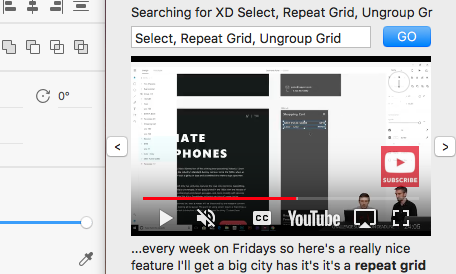
\includegraphics[width=\textwidth]{replay/figures/replay-old.png}
  \caption{Study 1 used this initial version of RePlay, shown here next to Adobe \textsc{xd}. It did not show video titles or timeline markers; instead it had arrow buttons next to each video to skip between that video's ranked clips. It also added the 3 most recent tools to the search query instead of one. }~\label{fig:replay-old}
%   \Description[A screenshot of an older version of RePlay.]{A screenshot of an older version of RePlay. Above the search field, the status area reads ``Searching for XD Select, Repeat Grid, Ungroup Grid''. Inside the search field it reads ``Select, Repeat Grid, Ungroup Grid''. It displays a video result with no title and a short caption excerpt underneath that includes the words ``repeat grid'' bolded.}
\vspace{-0.25in}
\end{figure}

\subsubsection{Contextual clip search was most useful for specific tasks}
Four participants said they tended to use RePlay when stuck trying to figure out how to do something specific. Three also said they used it to find out what a particular tool could do or how to use it. All but one participant worked on targeted tasks (see \autoref{table:study1_usage}). \textit{P3} wanted general resources for getting started with Sketch, and did not find RePlay helpful.

Three users recounted similar stories of searching for a particular question and quickly finding a clip within a video that answered it. \textit{P1} described searching for ``Make Symbol'' after clicking on the ``Make Symbol'' tool in Adobe \textsc{xd}. The answer he needed came from an auto-selected moment near the end of a 3-hour video. \textit{P1} added, \textit{``if I had searched for that myself I would've given up.''} Similarly, \textit{P5} found what he needed in a 1.5 hour video that was cued to a moment 20 minutes in. He was trying to create margins, and searched for ``layout grid'', and \textit{``The first video in the list showed me exactly what I needed to do''}, which was to check a box he hadn't noticed. \textit{P4} found RePlay useful for indicating that her specific goal was \textit{not} possible: she wanted to customize a grid system in Sketch and searched for ``grid settings'', but the caption excerpts indicated that none of the results mentioned customizing grids.

Contextual video clips sometimes invited opportunistic learning: \textit{P1} and \textit{P7} recounted instances where a video they were watching taught them something they didn't know and hadn't thought to look for. \textit{P1} continued watching the ``make symbols'' video as it described grouping and layering symbols. This part \textit{``wasn't originally what I was searching for but it was exactly what I needed ... [I] gained a lot more knowledge.''} \textit{P7} described how he \textit{``searched for `character styles' and actually found new information that I've never seen before''} about the Libraries panel.

\begin{figure*}[t!]
\centering
  \vspace{-0.2in}
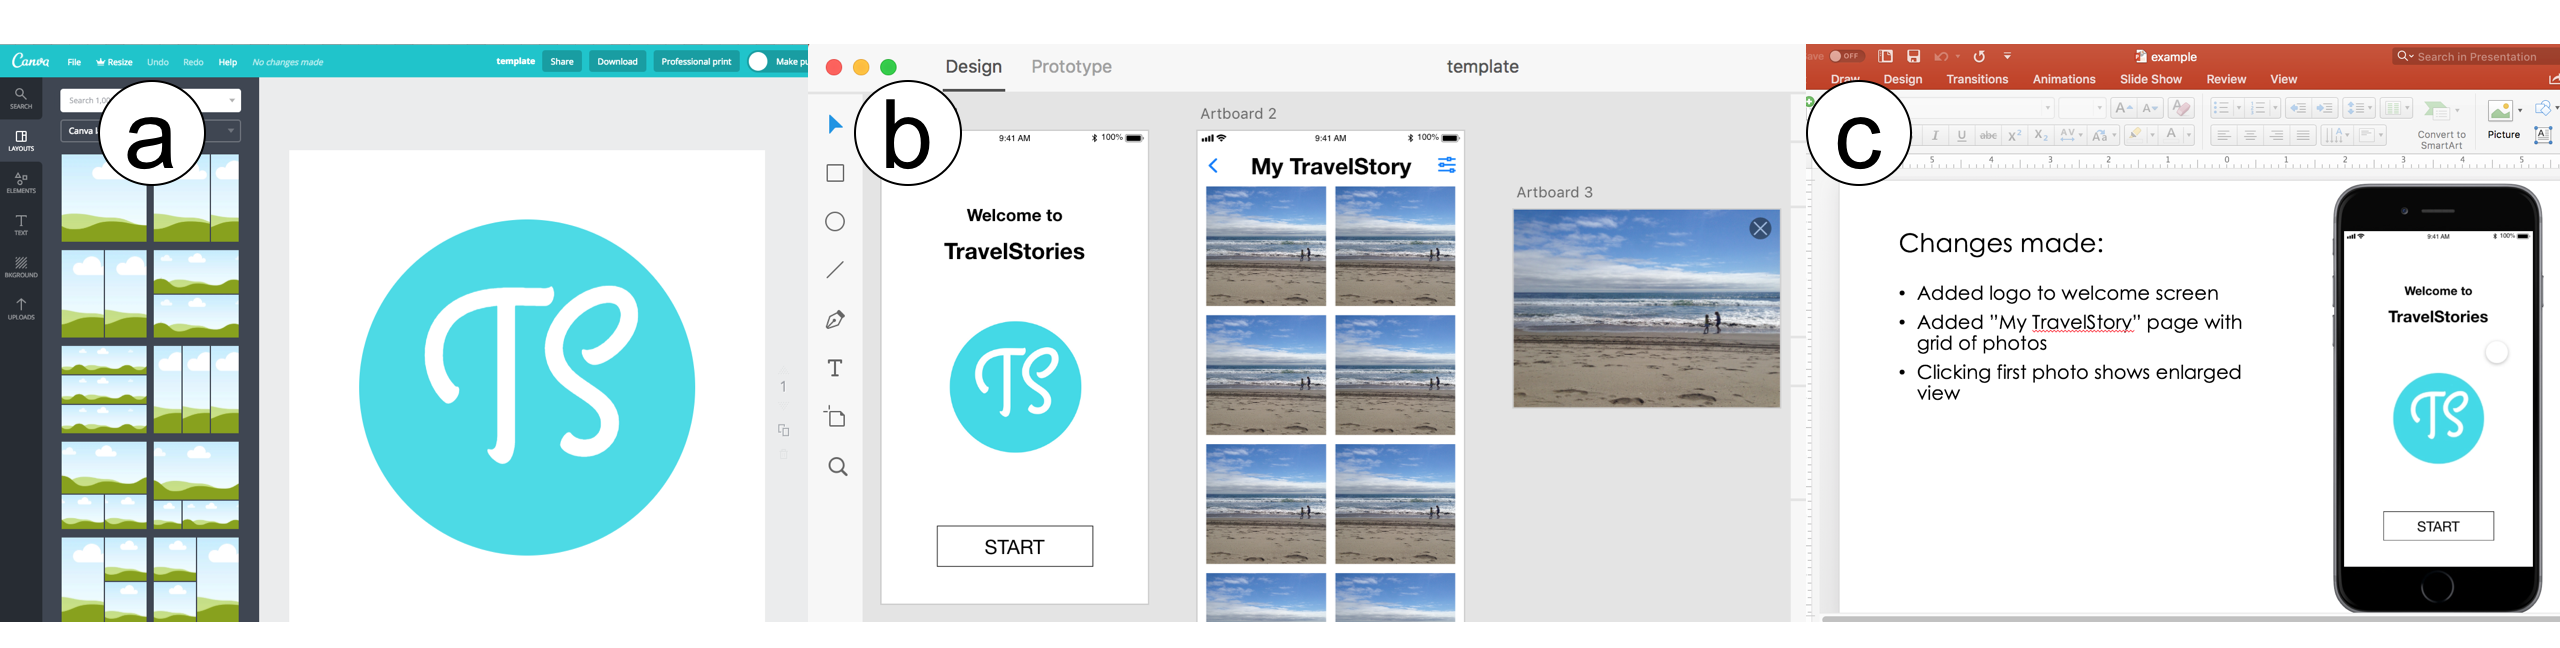
\includegraphics[width=\textwidth]{replay/figures/study2_task.png}
\vspace{-0.3in}
  \caption{Study 2 asked participants to make changes to an initial logo in Canva (a), update a prototype in Adobe \textsc{xd} (b), and make a presentation showing their changes in PowerPoint (c).}~\label{fig:replay-study2-task}
  \vspace{-0.2in}
%   \Description[Screenshots of the three template files participants were given.]{Screenshots of the three template files participants were given. The first is a blue circle with ``TS'' in the middle, shown in the Canva interface. The second is a wireframe design in Adobe XD with three phone screens, one that says ``Welcome to TravelStories'' with a Start button, one that says ``My TravelStory'' with a grid of photos below it, and one showing a photo at full size. The third is slide in PowerPoint with a screenshot of the wireframe on the right, and some text on the right that lists changes made to the design.}

\end{figure*}

%\vspace{0.1in}
\subsubsection{Tool context helps, but not in the search query}
All participants who searched with RePlay preferred deleting tool names from the query and instead typing their own. Five participants mentioned that including three tools in the query was too many, as it made the query too general. \textit{P3} said this was because the automatic query seemed \textit{``stuck on the last thing I did, which might not be relevant to what I'm thinking now.''} Both \textit{P4} and \textit{P5} said tool \textit{names} were not as useful because they wanted to search for an \textit{action}, not its constituent tools (\textit{e.g.,} ``rotate object'' or ``export nested artboard''). Higher-level activity inference may provide more useful assistance.

Two participants said they liked that RePlay populated the query with tool names because \textit{``coming up with the right search terms is really hard and I don't know the names of the tools [...] so it's nice not to have to think of them''} (\textit{P4}). Even \textit{P6}, the expert, said \textit{``I know how to use everything but if you asked me the names of the tools, I have no idea}.'' Participants appreciated that RePlay added the application name to the query, as it allowed them to \textit{``spend more brain power on the details of [the query]'' (P2)}. 

\subsubsection{Participants frequently switched between applications}
RePlay logged every time users switched between \textit{any} applications when it was running. Excluding system applications (such as Dock, Finder, and System Preferences), participants used an average of 17 different applications while RePlay was running ($SD\!=\!8$), and switched between applications a mean of every 6.6 minutes ($SD\!=\!8.5$min). If we exclude all continuous periods of over 3 hours (assuming that these sessions were breaks of some sort), this average lowers to every 2.5 minutes ($SD\!=\!1.8$min). This diverse app usage supports our motivation for supporting cross-app workflows.

\subsubsection{Improvements to RePlay}
Because participants thought that auto-including three tools was too many, Replay now includes only the most recent one. Four participants also mentioned that more general information like video titles would be helpful, as caption excerpts often seemed \textit{``out of context''} or \textit{``snatched out of middle of a sentence''} (\textit{P2}). Consequently, RePlay now includes video titles. Four participants wished they could watch videos at a larger size; RePlay now includes a resizable video player window. Two participants also mentioned that some video results did not pertain to the current application; RePlay now excludes results that do not mention the current application in the metadata or captions.

\section{Study 2: How does RePlay compare to current methods for video assistance?}

A between-subjects study ($n\!=\!24$) investigated how contextual assistance for multi-app activities might affect behavior compared to standard web video search. It found that contextual assistance can reduce time spent searching and navigating videos.

\subsection{Study procedure}
Participants were asked to imagine that they were designers working for a client developing a travel journal mobile app. To replicate a multi-app activity, the study task spanned three applications: Canva (\url{canva.com}), Adobe \textsc{xd}, and Microsoft PowerPoint. Participants were asked to improve and change an initial design for their client (\autoref{fig:replay-study2-task}). The task had both creative and technical requirements. Creative requirements included making the logo more travel-themed, adding visual appeal to the prototype welcome screen, and making a PowerPoint presentation to show to the client. Technical requirements included adding additional photos to a grid, rounding their corners, and recording a video walkthrough. If participants needed help, they were instructed to search for tutorial videos using either RePlay or YouTube in a web browser. RePlay participants were introduced to its features prior to the task. To ensure that all participants had access to the same resources, they were asked not to use other search engines or resources. Participants had 45 minutes to complete the task, and answered questions about their experience and help-seeking at the end. Participants were compensated with a \$15 gift card.

\subsubsection{Participants}
Twenty four participants (14 female) were recruited through online and paper advertisements on a university campus. Prior to the study, participants filled out a survey about their design experience. Participants were randomly assigned to either the RePlay ($n\!=\!12$) or Web ($n\!=\!12$) condition and counterbalanced based on experience. ``Novice'' was defined as completing at most two courses in design and reporting experience with at most two design applications. ``Experienced'' was defined as completing more than two courses in design or reporting experience with more than two design applications. Six of the 24 participants were ``experienced''. 

Participants rated their pre-study familiarity with each of the three study applications on a 5-point Likert Scale. Participants were generally familiar with Powerpoint ($mean\!=\!4.2$), and unfamiliar with Canva ($mean\!=\!1.5$) and Adobe \textsc{xd} ($mean\!=\!1.2$).
 
\subsubsection{Measures}
We were primarily interested in participants' search behavior. We measured the number of queries, their length, and time spent in the search interface. Qualitative measures included how participants determined which videos to watch and their navigation strategies (observed through screen recordings). We also gathered participant feedback in the RePlay condition on its features.

\subsection{Results}
RePlay participants averaged 3.3 queries each (33 total); Web participants averaged 3 queries each (24 total) ($x^2\!=\!1.42$, $df\!=\!1$, $p\!=\!.23$). Web participants typed longer queries ($mean\!=\!4.33$ words, $SD\!=\!1.41$) than RePlay participants ($mean\!=\!2.53$ words, $SD\!=\!0.59$)($t\!=\!2.52$, $df\!=\!15.98$, $p\!<\!.01$), because Web participants often manually added the application name, whereas RePlay auto-included it. 72\% of search queries were for Adobe \textsc{xd} and 28\% were for Canva; none were for PowerPoint since participants were more familiar with it. Four Web and two RePlay participants did not search for any assistance; we cover this in the Discussion.

Participants varied considerably in the amount of time and effort they spent. This is a challenge with a task that has both creative and technical components; people prioritize these components differently. Many participants spent a long time perfecting their design and had to be cut off after 45 minutes; others did the minimum required and finished in as few as 23 minutes. Because the task was open-ended, we did not compare completion times across participants. Our analysis focuses on search behavior. 

\begin{figure}[b!]
\centering
%\vspace{-0.25in}
  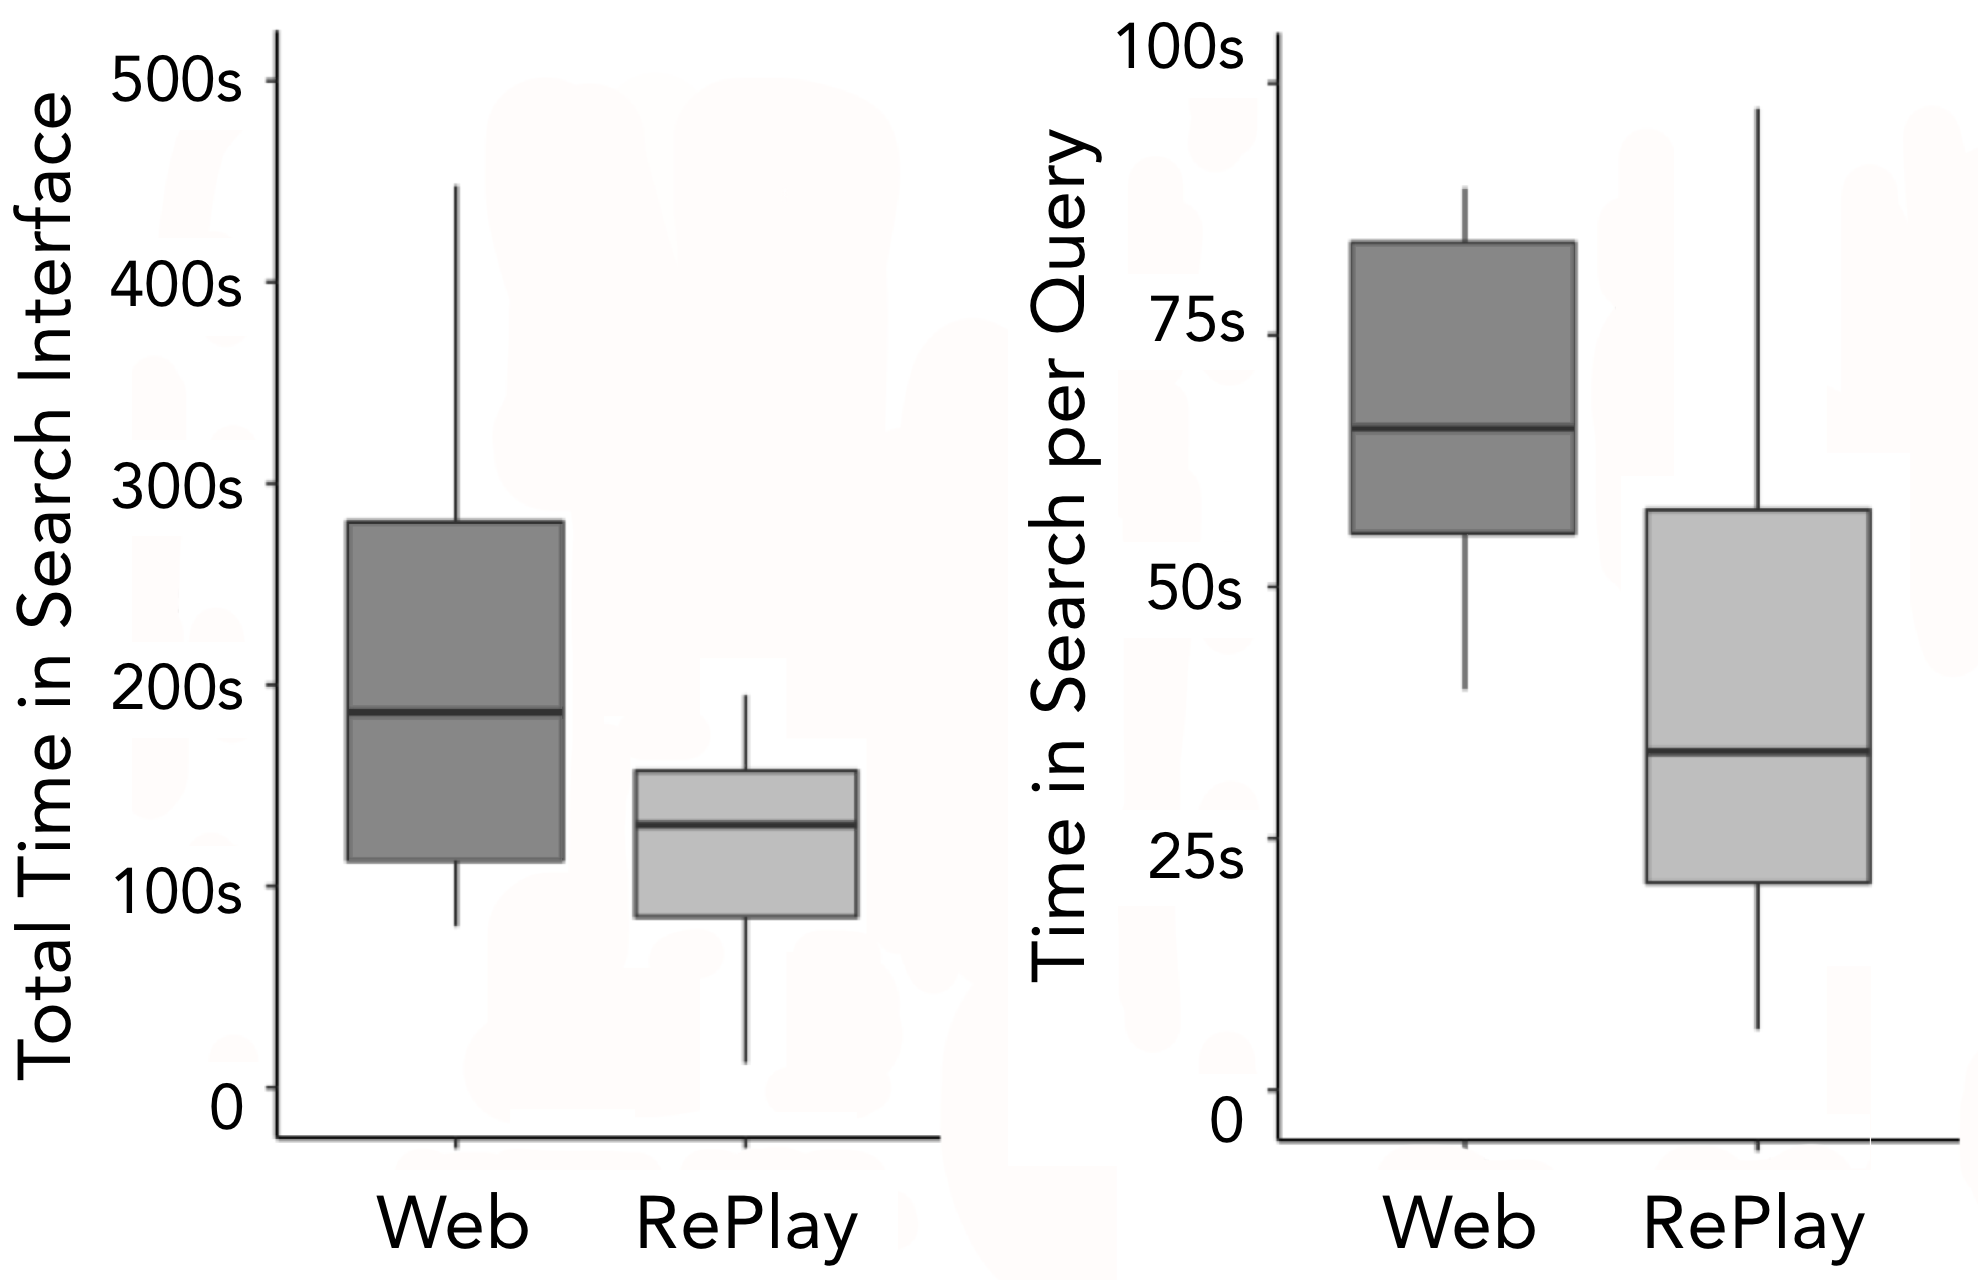
\includegraphics[width=1\textwidth]{replay/figures/study2_graphs.png}
  \caption{RePlay participants spent marginally less time overall in the search interface than Web participants ($p\!=\!.07$, left) and significantly less time \textit{per query} ($p\!=\!.02$, right).}~\label{fig:replay-study2-graphs}
  \vspace{-0.2in}
%   \Description[Two graphs showing the difference between RePlay and Web participants in time spent in the search interface.]{Two box plots showing the difference between RePlay and Web participants in time spent in the search interface. On the left, RePlay's box is slightly lower than Web's for total time in search (seconds). On the right, RePlay's box is significantly lower than Web's for time in search by query per person (seconds).}
\end{figure}

% Keep this somewhere? As a result, traditional completion time or completion rate are not suitable metrics. 

\subsubsection{Contextual assistance lessens time away from task}
Web participants spent nearly twice as long in the search interface ($mean\!=\!214.5$ seconds, $SD\!=\!127.1$) as RePlay ones ($mean\!=\!116.2$ seconds, $SD\!=\!58.9$). Due to the high variance and small sample size, the difference was marginally significant ($t\!=\!2.02$, $df\!=\!9.4$, $p\!=\!.07$) (\autoref{fig:replay-study2-graphs} left). When the time each participant spent in search is averaged by the number of queries they made, the difference is significant: RePlay participants spent about 40\% less time in search per query ($mean\!=\!42.83$ seconds, $SD\!=\!29.5$) than Web participants ($mean\!=\!72.62$ seconds, $SD\!=\!22.4$)($t\!=\!2.52$, $df\!=\!15.28$, $p\!=\!.02$) (\autoref{fig:replay-study2-graphs} right). Though RePlay pre-cached many video captions beforehand, we could not predict all queries users would make. Thus, some query responses in RePlay took up to two minutes. Because this latency could be reduced, we subtracted loading times in both conditions from the total time in search.

Easier navigation both within and between video results may explain why RePlay participants spent less time in the search interface per query. Web participants used various strategies for navigating within videos, including keyboard shortcuts to fast-forward and rewind, increasing video speed, and hovering over the timeline. Navigating between different video results in YouTube required selecting a video, watching or skipping through it to determine whether it was relevant, and if not, going back to the results page and selecting another. RePlay's timeline markers replaced many of these strategies, increasing efficiency: participants could first examine the timeline markers before deciding if and at what point to watch a video result. Eight RePlay participants hovered over timeline markers to read the caption previews, often hovering over multiple points before deciding where to watch. RePlay's panel interface also enabled participants to simultaeously play one video and examine others. We observed three participants do this, likely to decide whether another video was better without giving up on their first choice. One such participant said they wished for better visual cues of video relevance to help decide which to watch. Other participants browsed videos one at a time, perhaps to focus on the playing video.

% \begin{figure}[b!]
% \vspace{-0.25in}
% \centering
%   \includegraphics[width=0.9\textwidth]{replay/figures/study2_avgsearch.png}
%   \caption{Web participants spent significantly longer in the search interface \textit{per search query} than RePlay participants ($p=.02$). }~\label{fig:replay-study2-avgsearch}
% \end{figure}

\subsubsection{Search queries were action-oriented, not tool-oriented}
As in Study 1, participants removed tool names from queries. No participants in either condition used tool names. Instead, participants wrote action-oriented queries: the most common were ``crop photos'', ``round corners'', and ``record video.'' Despite RePlay adding the current tool name to the search field, in all instances but one, participants deleted the tool name from their query.

\begin{table}[t]
%\vspace{-0.35in}
\begin{tabular}{lllll}
\textit{RePlay Feature} & Title                   & Thumbnail               & Caption                 & Timeline                \\ 
\textit{Helpfulness}    & \multicolumn{1}{c}{2.8} & \multicolumn{1}{c}{3.1} & \multicolumn{1}{c}{2.5} & \multicolumn{1}{c}{4.2}
\end{tabular}
\caption{Average helpfulness ratings for RePlay's contextual features ($n\!=\!12$). Most participants found the timeline markers most helpful for determining which videos to watch.}~\label{table:study2_replayfeatures}
\vspace{-0.3in}
\end{table}

\subsubsection{Intra-video context is most helpful}
In interviews, participants rated timeline markers as the most helpful (4.2/5) (\autoref{table:study2_replayfeatures}). RePlay participants hovered over timeline markers a total of 69 times and clicked on markers 22 times. One participant mentioned that timeline markers provide a \textit{``scaffold of what to look for and where to start watching.''} Participants rated caption excerpt and video title as less helpful. A few participants mentioned ignoring titles and excerpts in favor of timeline markers and video thumbnails. Twice in each condition, participants selected the first video result even though the title mentioned the wrong application (Photoshop or Illustrator). This suggests that the video region is a strong magnet for people's attention.


%Tasks that require a context switch are perceived to take longer than tasks that don't. 
%Intra-person effect size for search interfaces is smaller than inter-person differences. To see the impact of search interfaces, need large n.
% One motivation for having the app do searching for you is that people aren't good at it. 

% Another participant found the timeline markers helped them \textit{extrapolate form the video where I should search for the content that I'm looking for. And it that one doesn't have it, I can just skip through and see other [points].''} general, participants found this feature helpful (4.11 rating on 5-point Likert scale). 
\section{Discussion \& Future Work}
Observations and feedback from the two studies suggest several opportunities for future work. 

\subsection{How Can Contextual Assistance aid Exploration?}
% assistance should not discourage exploration, but intervene when it is needed
% people explore because incremental cognitive load of exploration is small
% search is a one-time switch cost. if we can make the switching cost lower (by embedding in app and adding context) this should increase usage, and leaves people with more registers to focus on what they want to do.

Study 2 participants often preferred manually exploring when it would have been more efficient to search for help. The study's subjective, open-ended task may have encouraged such exploration. Only one participant used the best method to update the photo grid - using Adobe \textsc{xd}'s repeat grid feature to update all photos simultaneously - after learning about it in a video. Other participants used various less-efficient methods (\textit{e.g.}, un-grouping the repeat grid and manually adding and re-sizing photos). Because these methods achieved their desired goal, participants may not have thought to investigate whether a faster option existed.

Interface exploration and browser search each have shortcomings. Exploration is a common problem-solving strategy because it can be enjoyable, it builds on domain knowledge, and each individual action is low cost \cite{Lafreniere2014a, Rieman1996}. However, for novices especially, exploration is cumulatively slow, its learned knowledge is hard to integrate, and it induces a high cognitive load \cite{Tuovinen1999, Lafreniere2014a}. A limitation of learning unfamiliar domains via exploration is that people may settle for sub-optimal methods or strategies because they are unaware of a better alternative. Moving from an application to a web search can yield better results, but has a higher initial cost as it lurches people out of their task. We believe that contextual search has the potential to offer the benefits of both approaches without either of the drawbacks. 

Six participants in Study 2 did not search at all; most felt they could figure things out via exploration. One participant said they \textit{``felt like I could find it if I searched for it [in the interface], which I did. I was able to figure it out.''} Two other participants mentioned that they felt searching for help would be more time-consuming than trial-and-error exploration. One stated that he wanted to search for help, but \textit{``I knew I didn't have time. I wanted to complete the task so I just hacked it.''} If Study 2's result that contextual search reduces search time holds, these perceptions may change over time. RePlay's occasionally-slow loading times may have also affected this perception; prior work shows that a difference in latency of search results as small as 300ms can discourage people from searching \cite{Brutlag2009}.

How might contextual assistance encourage productive exploration while providing intervention when needed? While proactive support can be beneficial, a challenge is providing assistance without being too disruptive \cite{Matejka2011}. To minimize distractions, the RePlay interface mostly changes only in direct response to user input. However, novices may not even realize they need help, making proactive suggestions more valuable. For example, RePlay could automatically refresh video results when the user seems stuck, or suggest relevant queries when the user begins to search. Future work should examine how these alternatives might change people's behavior and workflows over time.
%will having assistance readily available change behavior over time? people have learned to guess their way to the solution and this is good in a lot of ways. but is there some interesting potential around a categorical strategy/behavior shift
% One Web participant said that he \textit{``almost always won't watch video because it's time-consuming...I usually prefer text-based help.''}. Similarly, another participant preferred text because \textit{``it's easier to parse rather than searching through a video.''} 

\subsection{What and How Much Context to Include?}
While logging recent tools can help suggest next steps \cite{Matejka2009}, we found that using recent tools explicitly in search queries is not useful. Participants in both studies did not use tool context in their queries, preferring action-oriented queries instead. Usage history is by definition retrospective (\textit{i.e.}, it describes what the user has already done). In contrast, search is often prospective (\textit{i.e.}, looking for something the user hasn't done yet). Tool context may only be helpful closer to where users interact with tools (\textit{e.g.,} as part of tooltips \cite{Grossman2010a}).
%can help divulge this information to users by increasing tools' information scent \cite{Pirolli2009}.

Interestingly, people used the same terms and concepts across different applications. Study 2 participants searched ``crop photos'' for both Canva and Adobe \textsc{xd} despite neither application having an explicit crop tool. This highlights both a challenge and an opportunity: people bring mental models that may not carry over into different applications. Study 1 suggested that displaying tool names may help people learn app-specific terminology. However, for both knowledge and speed reasons, users sometimes omit valuable terms. RePlay's interface benefits are reduced when users don't search using the same terms as videos. A natural language mapping \cite{Adar2014} between video captions (along with other natural language data like comments and tags) and the tools they mention may increase captions' value for search.

Finally, what other contextual information besides tool use might be helpful for identifying relevant videos? Liu \textit{et al.} \cite{Liu2020} showed that in addition to command logs, information about the use of layers and the time between interaction events can help segment usage logs from image editing tasks into subtasks. Similarly, information such as the name of the user's active layer might be helpful as additional context for a search query. Liu \textit{et al.} also found that the visual change and location of the user's edits were less useful for segmentation, but perhaps the visual content of the user's canvas or document could be used to identify videos with similar content. Future work should explore how we might collect and use such types of contextual information to search for help in an application-general way.

\subsection{What Design Challenges Remain?}
Many design decisions were motivated by our focus on cross-application workflows; \textit{e.g.,} showing results in a separate window in a consistent location. Showing all results together made it easy to browse multiple resources at once. However, some participants still preferred focusing on one video at a time. Future work should consider how different layouts influence browsing behaviors and which behaviors lead to more effective workflows.

Currently, users must explicitly whitelist an application for RePlay to capture its events. While this approach offers more privacy, it also adds burden for users.  Blacklisting, on the other hand, would allow RePlay to respond to all applications except for explicitly-omitted potentially-sensitive ones (\textit{e.g.,} Messages), offering broader benefits. For our initial studies, we chose the greater privacy of a whitelist. For real use, users could choose whitelist or blacklist, and/or RePlay could request approval for each new application, similar to websites that ask for a user's location.

\subsection{What Other Domains Might Benefit?}
RePlay's main insight is that given a source of user context, we can search, curate, and index into resources from a large corpus. RePlay demonstrates this approach using video; different activities (\textit{e.g.,} programming) may benefit from other types of content (\textit{e.g.,} text resources). RePlay could naturally be extended to any textual resource (or resource with textual metadata). Text results could be displayed as short summaries with clickable keywords to expand more detail~\cite{Ekstrand2011}. For detecting context, RePlay used Mac\-OS's accessibility \textsc{api}; other \textsc{os}s (\textit{e.g.} Windows \cite{Matejka2013}) also have similar \textsc{api}s. %Minor differences should not significantly affect RePlay's approach, as the user's query is still the primary search input.
Beyond software, RePlay's approach could extend to any domain for which online videos are abundant (\textit{e.g.,} physical building tasks). To detect activity context, one could augment physical tools with sensors \cite{Schoop2016, Lukowicz2004} or track body poses with wearable sensors or computer vision. A challenge for future work is to convert sensor or vision data into text searches, or to index videos using the sensor or vision data directly. 

% We used the application name, but the domain of the user's task may also be important for narrowing down results regarding multi-functional applications like Photoshop or Powerpoint.

% first study had a lot of retrospective context, was not helpful
% usage histor/state is retrospective and not always helpful for prospective search -- how address this without being clippy?
% eric horovitz
% how move forward with this and not end up with clippy? how to have good mixed initiative support?
% proactive variations: generate alternatives automatically and show them to you i already did it
% what about proactively suggesting search queries instead of videos/resources?

%All three participants in our field study almost exclusively typed their own search queries rather than using the ones RePlay provided. Using multiple recent tools explicitly in a search query takes the focus away from the specific question or tool the user wants help with. An alternative approach (suggested by \textit{P1}) could instead show recent tools as clickable elements for quick searches, while also providing a search box for user-generated queries.

% Future work: use prefab methods to get visual stuff too, could search with that

% \subsection{The First Result is Most Relevant for Context}
% Effective search interfaces should not only present relevant results, but also present the most relevant results at the top of the set [Hearst]. As we observed in Study 2, people tend to habitually choose the first result provided, expecting it to contain the most relevant information needed.

\section{Conclusion}
This paper introduced an application-independent approach for contextually presenting videos and a demonstration of this approach in the RePlay system. RePlay shows how system accessibility features and video captions can be used to detect context and search within videos in a flexible, domain-general way. Like curb cuts or closed captioning \cite{Rose2002}, RePlay demonstrates how accessibility features can provide universally-beneficial assistance. 
Expanding accessibility and increasing cross-app consistency through guidelines and enforcement would benefit everyone. It would also expand application tailoring, integration, and assistance with systems like RePlay. Two studies demonstrated that cross-app contextual video assistance helps users spend more time on their task and less time searching for help. We also observed how contextual assistance can sometimes be at odds with peoples' desire to explore and tinker, and that the context most easily accrued from software usage may not always be the most relevant. Future work should investigate these challenges and examine how contextual help affects workflows in the real world through a longitudinal study. This work brings us one step closer to leveraging the wisdom of the Web for personalized, just-in-time learning.

\section{Acknowledgments}
We are thankful to Michelle Lee for her assistance in conducting Study 2, and to all study participants for their time and feedback. This work was supported in part by NSERC and Adobe Research.


% % Load basic packages
% \usepackage{balance}       % to better equalize the last page
% \usepackage{graphics}      % for EPS, load graphicx instead 
% \usepackage[T1]{fontenc}   % for umlauts and other diaeresis
% \usepackage{txfonts}
% \usepackage{mathptmx}
% \usepackage[pdflang={en-US},pdftex]{hyperref}
% \usepackage{color}
% \usepackage{booktabs}
% \usepackage{textcomp}

% % Some optional stuff you might like/need.
% \usepackage{microtype}        % Improved Tracking and Kerning
% % \usepackage[all]{hypcap}    % Fixes bug in hyperref caption linking
% \usepackage{ccicons}          % Cite your images correctly!
% % \usepackage[utf8]{inputenc} % for a UTF8 editor only

% If you want to use todo notes, marginpars etc. during creation of
% your draft document, you have to enable the "chi_draft" option for
% the document class. To do this, change the very first line to:
% "\documentclass[chi_draft]{sigchi}". You can then place todo notes
% by using the "\todo{...}"  command. Make sure to disable the draft
% option again before submitting your final document.
% \usepackage{todonotes}
\chapter{ReMap: Multimodal Help-Seeking}
\label{chapter:remap}
\begin{quote}
People are reluctant to search for help when they feel it will take more time than trial-and-error exploration, even with a contextual search system like RePlay. However, trial-and-error often takes a long time or does not result in a correct solution. Given this cognitive bias, how might we lower the barrier to searching for help? This chapter aims to make searching easier and faster through multimodal interaction. We introduce \textit{ReMap}, an extension to the RePlay system that allows users to speak search queries, adding app-specific terms deictically. Users can navigate ReMap's search results via speech or mouse. A lab study showed that ReMap helped people stay focused on their task while simultaneously searching for and using help resources. Users' experiences with ReMap also raised a number of important challenges with incorporating multimodal features into a help-seeking system.
\end{quote}

\section{Introduction}
Despite the ubiquity of online search, help-seeking remains a tedious and difficult process for many. While the Web is ripe with knowledge and expert help, using it requires switching mental context, visual attention, and input focus away from the task at hand. As the RePlay study showed, these drawbacks often prevent people from searching altogether. Though bringing the search interface closer to the user's workflow and tying in relevant context seemed to help people spend less time once they decided to search, there was still an initial barrier that prevented many from searching in the first place. 
Coming up with an appropriate search query can be prohibitively difficult for novices, who may not know the correct vocabulary [dan russell]. It also switches the user's attention from the task at hand to the task of articulating their goal in a way that will match the resources they seek. How might we lower the barrier to searching and make it easier for people to find the resources they need in the moment?

When people help each other, they often use language, gestures, and context. Our research investigates how computers might do this too. The combination has allowed people of different backgrounds to communicate information and interact. Although it is a habit of humans to incorporate language, gestures, and context into assisting others, computers do not develop this knowledge unless programmed to. 

This chapter explores how multimodal interaction might make searching easier in the moment. Different types of information lend themselves better to different modalities; leveraging the strengths of multiple modalities and integrating them smoothly can be extremely effective \cite{Oviatt1999}. For example, combining speech and pointing allows people to communicate more precisely and efficiently by using deictic terms (\textit{e.g.,} ``this'', ``here'') to refer to objects and locations \cite{Bolt1980, Linder2013}. Furthermore, using multiple modalities simultaneously can improve efficiency; \textit{e.g.,} navigating tutorial videos with speech while one's hands are busy with a physical task \cite{Chang2019}. Finally, multimodal systems can also enable more natural interaction; \textit{e.g.,} letting users describe photo edits in their own words and inferring the appropriate commands \cite{Linder2013}, or activating software commands with speech rather than memorizing keyboard shortcuts \cite{Kim2019}.

\begin{figure}
\centering
  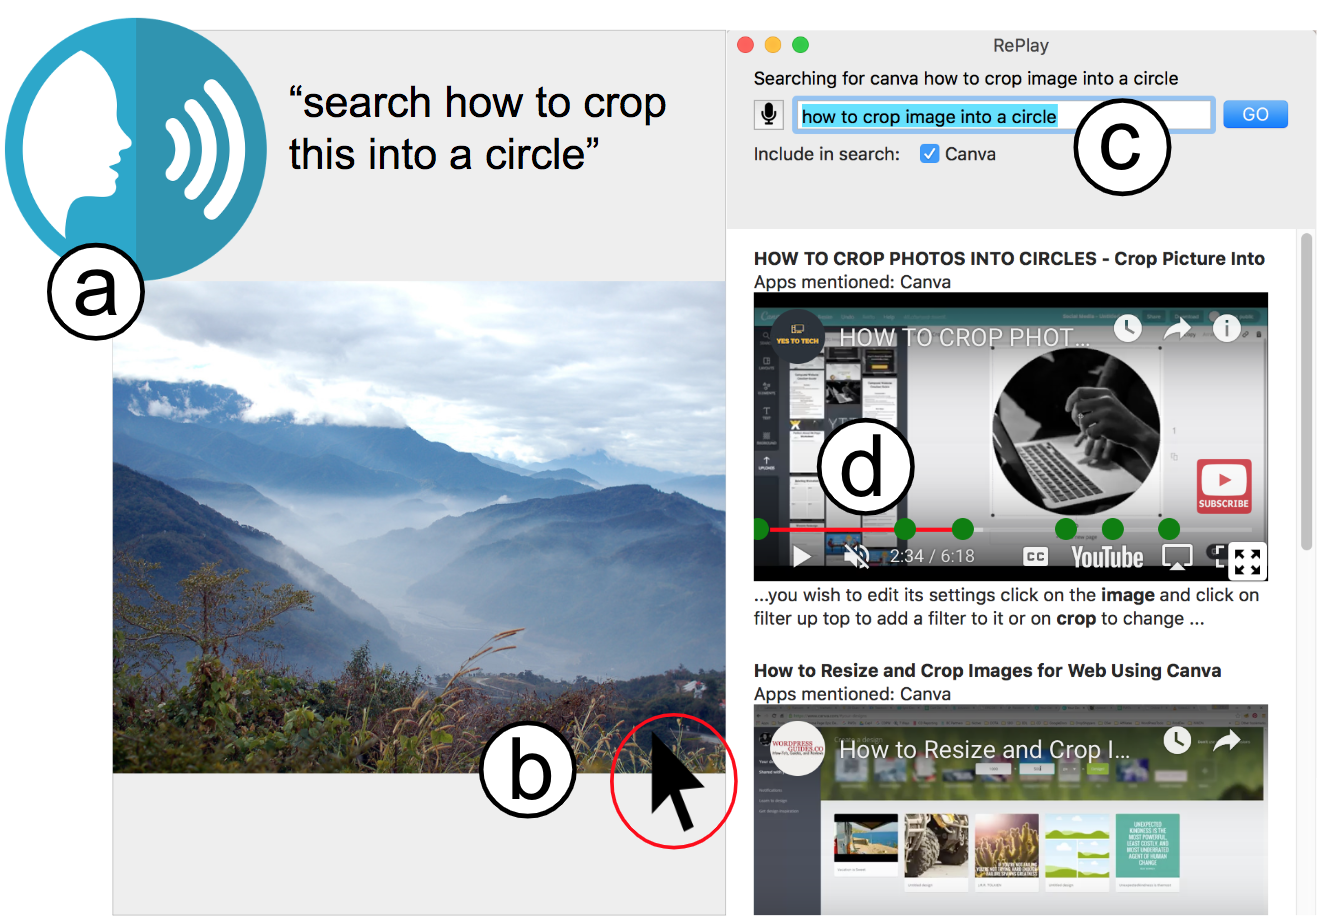
\includegraphics[width=\textwidth]{remap/figures/interface.png}
  \caption{ReMap is a multimodal search interface for finding learning videos. a) The user speaks their query. b) The user clicks on an image on the canvas while saying the word ``this.'' c) ReMap automatically changes the word ``this'' to ``image.'' d) ReMap highlights relevant moments by placing markers on the timeline of each video result.}~\label{fig:remap_interface}
  \vspace{-0.3in}
\end{figure}

We introduce ReMap, a multimodal interface for users to search for learning videos using speech and pointing, without taking their hands (or mouse) off their current task. ReMap builds on the existing video search interface RePlay \cite{Fraser2019}. ReMap's multimodal help search demonstrates three main design insights:
\begin{enumerate}
\item Users can initiate and dictate a search at anytime using speech, to avoid context-switching.
\item Users can point at elements in the software they are using to include their names in the search query, removing the need to remember app-specific terminology.
\item Users can play, pause, and navigate video results using speech, allowing them to simultaneously work on their task and follow along with a video tutorial.
\end{enumerate}

A study with 13 participants found that ReMap allows people to stay focused on their task while help-seeking. The study along with iterative prototyping and pilot testing also raised a number of important challenges with incorporating multimodal features into a help-seeking system.
\section{Related Work: Multimodal Interaction}
\subsection{The Power of Speech}
In 2016, Google reported that 20\% of all search queries on mobile Android devices were spoken \cite{Pichai2016}; that number has likely grown. Speech input is especially appealing on mobile devices, as people often use them while on the go and busy with other tasks \cite{Guy2016}, but even on desktop computers, voice assistants are often used for web search \cite{Mehrotra2016}. Speaking a search query is often easier and faster than typing it out, and it allows the user to ask a question like they might to a friend: mobile voice queries tend to be closer to natural language and more often phrased as questions than text queries \cite{Guy2016}. Also, people tend to search by voice more when seeking audio or video results \cite{Guy2016}, supporting ReMap's approach of using speech to search for videos. Finally, speech may be more useful for users with specific goals: Laput et al. \cite{Laput2013} found that when editing photos, speech was most useful when people knew exactly what they wanted to do. When people didn't know what they wanted, browsing a gallery of examples was more helpful as it allowed them to compare visual previews of potential effects before choosing one. Our studies with RePlay found that it was similarly most helpful for people with targeted questions, so we hypothesize that speech may be a useful way to search for help in ReMap.

\subsection{Combining Modalities can Maximize Cognitive Abilities}
Combining input from multiple modalities (\textit{e.g.}, speech, gesture, touch) can reduce cognitive load for complex tasks \cite{Oviatt2015, Reeves2004}, make tedious tasks more efficient \cite{Oviatt1999, Salisbury1990, Karl1993, Hugunin1997}, reduce errors \cite{Oviatt1999}, increase precision \cite{Cohen1989}, and even make tasks more enjoyable \cite{Oviatt1999, Laput2013}. Such combinations work best when they maximize users' working memory by using different modalities for different types of information \cite{Oviatt2015, Kalyuga1999, Reeves2004, Stanney2004}. 
%Auditory output is helpful for giving the user information while they work \cite{Stanney2004, Grossman2007, Reeves2004}, and visual output and manual input are helpful for conveying spatial information \cite{Stanney2004, Reeves2004}. 
For example, telling the user about keyboard shortcuts for the commands they execute via auditory feedback increases the likelihood that users will retain them, as users' auditory working memory is otherwise unused when working in software \cite{Grossman2007}. Similarly, using speech to navigate tutorial videos while one's hands are busy with a physical task allows users to process both the video and the task simultaneously \cite{Chang2019}. ReMap similarly partitions different modalities between the user's creative task and ReMap's help-seeking interface (\autoref{fig:remap_modalities}), allowing users to speak search queries and commands for navigating videos.

\begin{figure}[t]
\centering
  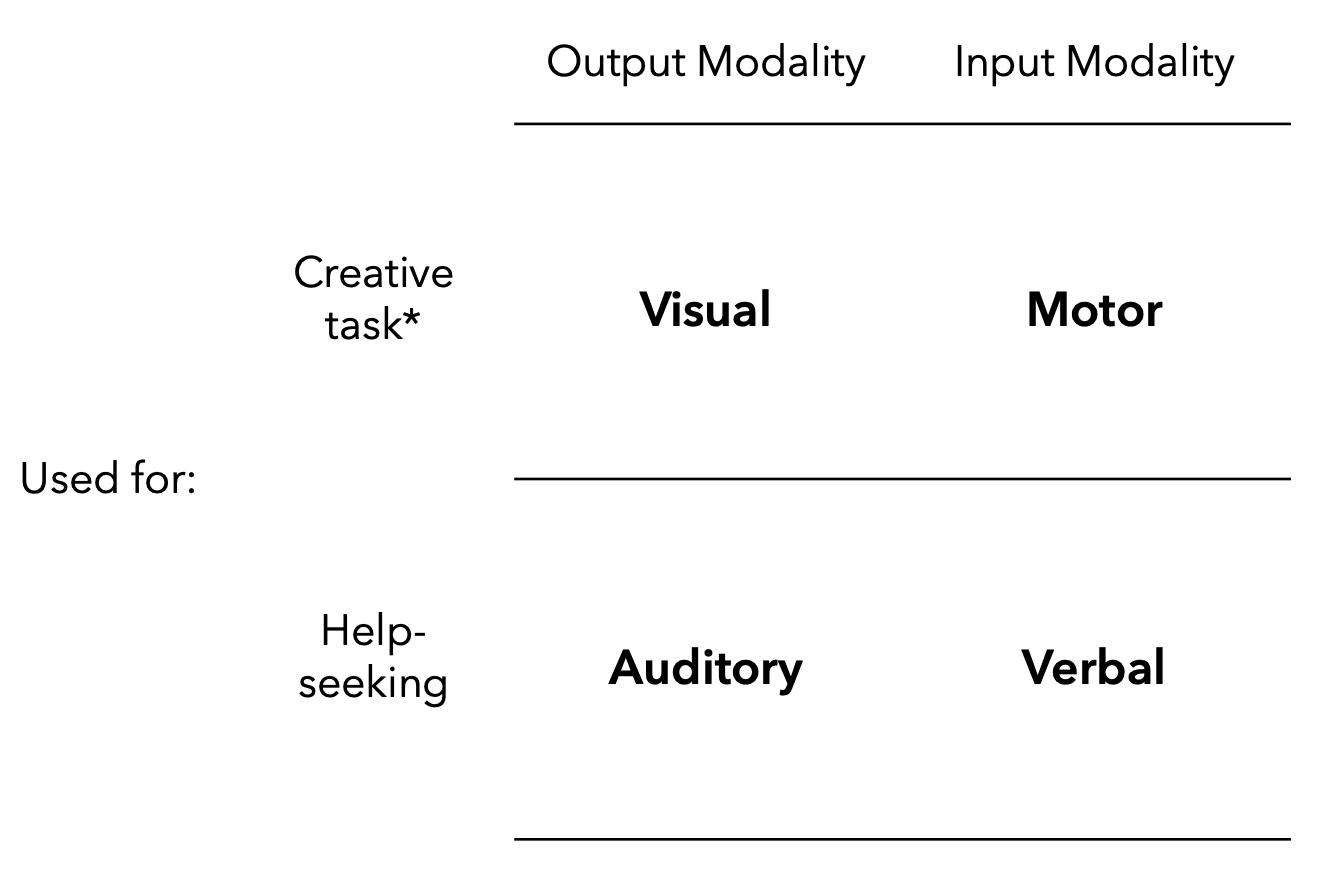
\includegraphics[width=0.7\textwidth]{remap/figures/remap_modalities.png}
  \caption[ReMap partitions the above modalities between the user's creative task and their help-seeking task to maximize cognitive abilities. Users primarily use speech and listening to search for and navigate help videos while keeping their hands and eyes on their creative task.]{ReMap partitions the above modalities between the user's creative task and their help-seeking task to maximize cognitive abilities. Users primarily use speech and listening to search for and navigate help videos while keeping their hands and eyes on their creative task. The * indicates that the visual and motor modalities are not \textit{exclusively} used for the creative task; users can also transfer their visual and motor attention to the help resources when necessary, \textit{e.g.}, to watch a video or type a search query manually.}~\label{fig:remap_modalities}
\end{figure}

Pointing at objects and spatial locations is often easier and more natural than describing them in words only \cite{Reeves2004, Bolt1980, Larkin1987}. Similarly, using a screenshot of an interface element as a search query is easier than describing it in text \cite{Yeh2009}. When combined with speech, pointing allows people to communicate more precisely by using deictic terms (\textit{e.g.,} ``this'', ``here'') to refer to objects and spatial locations while pointing at them \cite{Bolt1980, Laput2013}. ReMap similarly allows users to point at interface elements and canvas objects in their creative software and reference them deictically while speaking a search query.

Multimodal input can be especially beneficial for creative tasks, where maintaining a flow state is important. Using different modalities for software-related actions allows users to keep their focus and hands on their creative work. For example, using speech to access commands instead of menus or keyboard shortcuts can help artists maintain creative flow and stay focused on their task \cite{Kim2019, Sedivy1999}. While doing digital painting, an artist could switch from the brush tool to the eraser by saying ``eraser'' instead of switching their attention and moving their hands to the toolbar or keyboard \cite{Kim2019}. Not surprisingly, much prior work exploring multimodal input has centered around creative tasks such as photo editing \cite{Laput2013}, graphic design \cite{Kim2019}, drawing \cite{Sedivy1999, Pausch1991}, data visualization \cite{Setlur2016}, and 3D modeling \cite{Sharma2011}. However, most of this prior work has used speech to execute commands, rather than issue search queries. This requires either defining a list of acceptable commands (which users must then memorize) or parsing natural language commands (which is prone to errors). This chapter combines insights from multimodal creative systems and voice search systems to explore how voice search might be useful in creative software.

\section{ReMap System Design and Implementation}
ReMap (\autoref{fig:remap_interface}) extends the RePlay contextual search system \cite{Fraser2019}. RePlay enables users to search for learning videos in context while working in software, and it highlights relevant moments in video results based on the user's context and query. While RePlay helps people find results faster, the attentional cost of switching to RePlay discouraged its being used as often as it could. ReMap lowers the switching cost and load by introducing three main improvements over RePlay: searching for help using speech, making deictic references in a search query, and navigating video results using speech commands.

\subsection{Searching for help using speech}
ReMap uses the Web Speech \textsc{api} to detect speech by opening a browser page in the background when launched. This page can be minimized or hidden by the user. The first time it opens it asks the user to grant access to the microphone; all subsequent uses will grant access automatically. The page's JavaScript invokes continuous listening and sends the current phrase to ReMap's custom web server whenever a new word is detected.
The Web Speech \textsc{api} automatically determines when the user starts and finishes speaking, returning each phrase separately. If a phrase begins with the word \textit{``search''}, ReMap initiates a search (\autoref{fig:remap_interface}a), using the rest of the phrase as the query. Otherwise, it checks if the phrase matches any video navigation commands. If it does not, ReMap ignores it.

\subsection{Making deictic references in a search query}
Especially with new software, people are often unfamiliar with an application's vocabulary but can point at application elements that are relevant to their goal. 
To alleviate the challenge of remembering app-specific terms, ReMap allows users to deictically reference interface elements and objects while speaking their query. If the user says \textit{``this''} or \textit{``that''} while clicking on a detectable element, ReMap replaces the pronoun with the reference element's name (\autoref{fig:remap_interface}b-c). Like RePlay, ReMap uses the MacOS Accessibility \textsc{api} to resolve element names. 
%This \textsc{api} can get the name and description of any element with accessibility labels \cite{Fraser2019}. Many modern applications have labeled menus, buttons, and other interface elements. Some also label canvas elements (such as text boxes, images, and graphics) though many do not. The examples in this demo use Canva (\url{canva.com}) as the primary software. Canva labels most canvas elements and interface buttons.

While ReMap is detecting a speech query, it stores a list of every detectable element clicked. Once the user is finished speaking and ReMap has obtained the final query from the server, it replaces all occurrences of \textit{``this''} and \textit{``that''} with the element names in the order they were clicked before issuing the search query.

\begin{figure}[b!]
\centering
  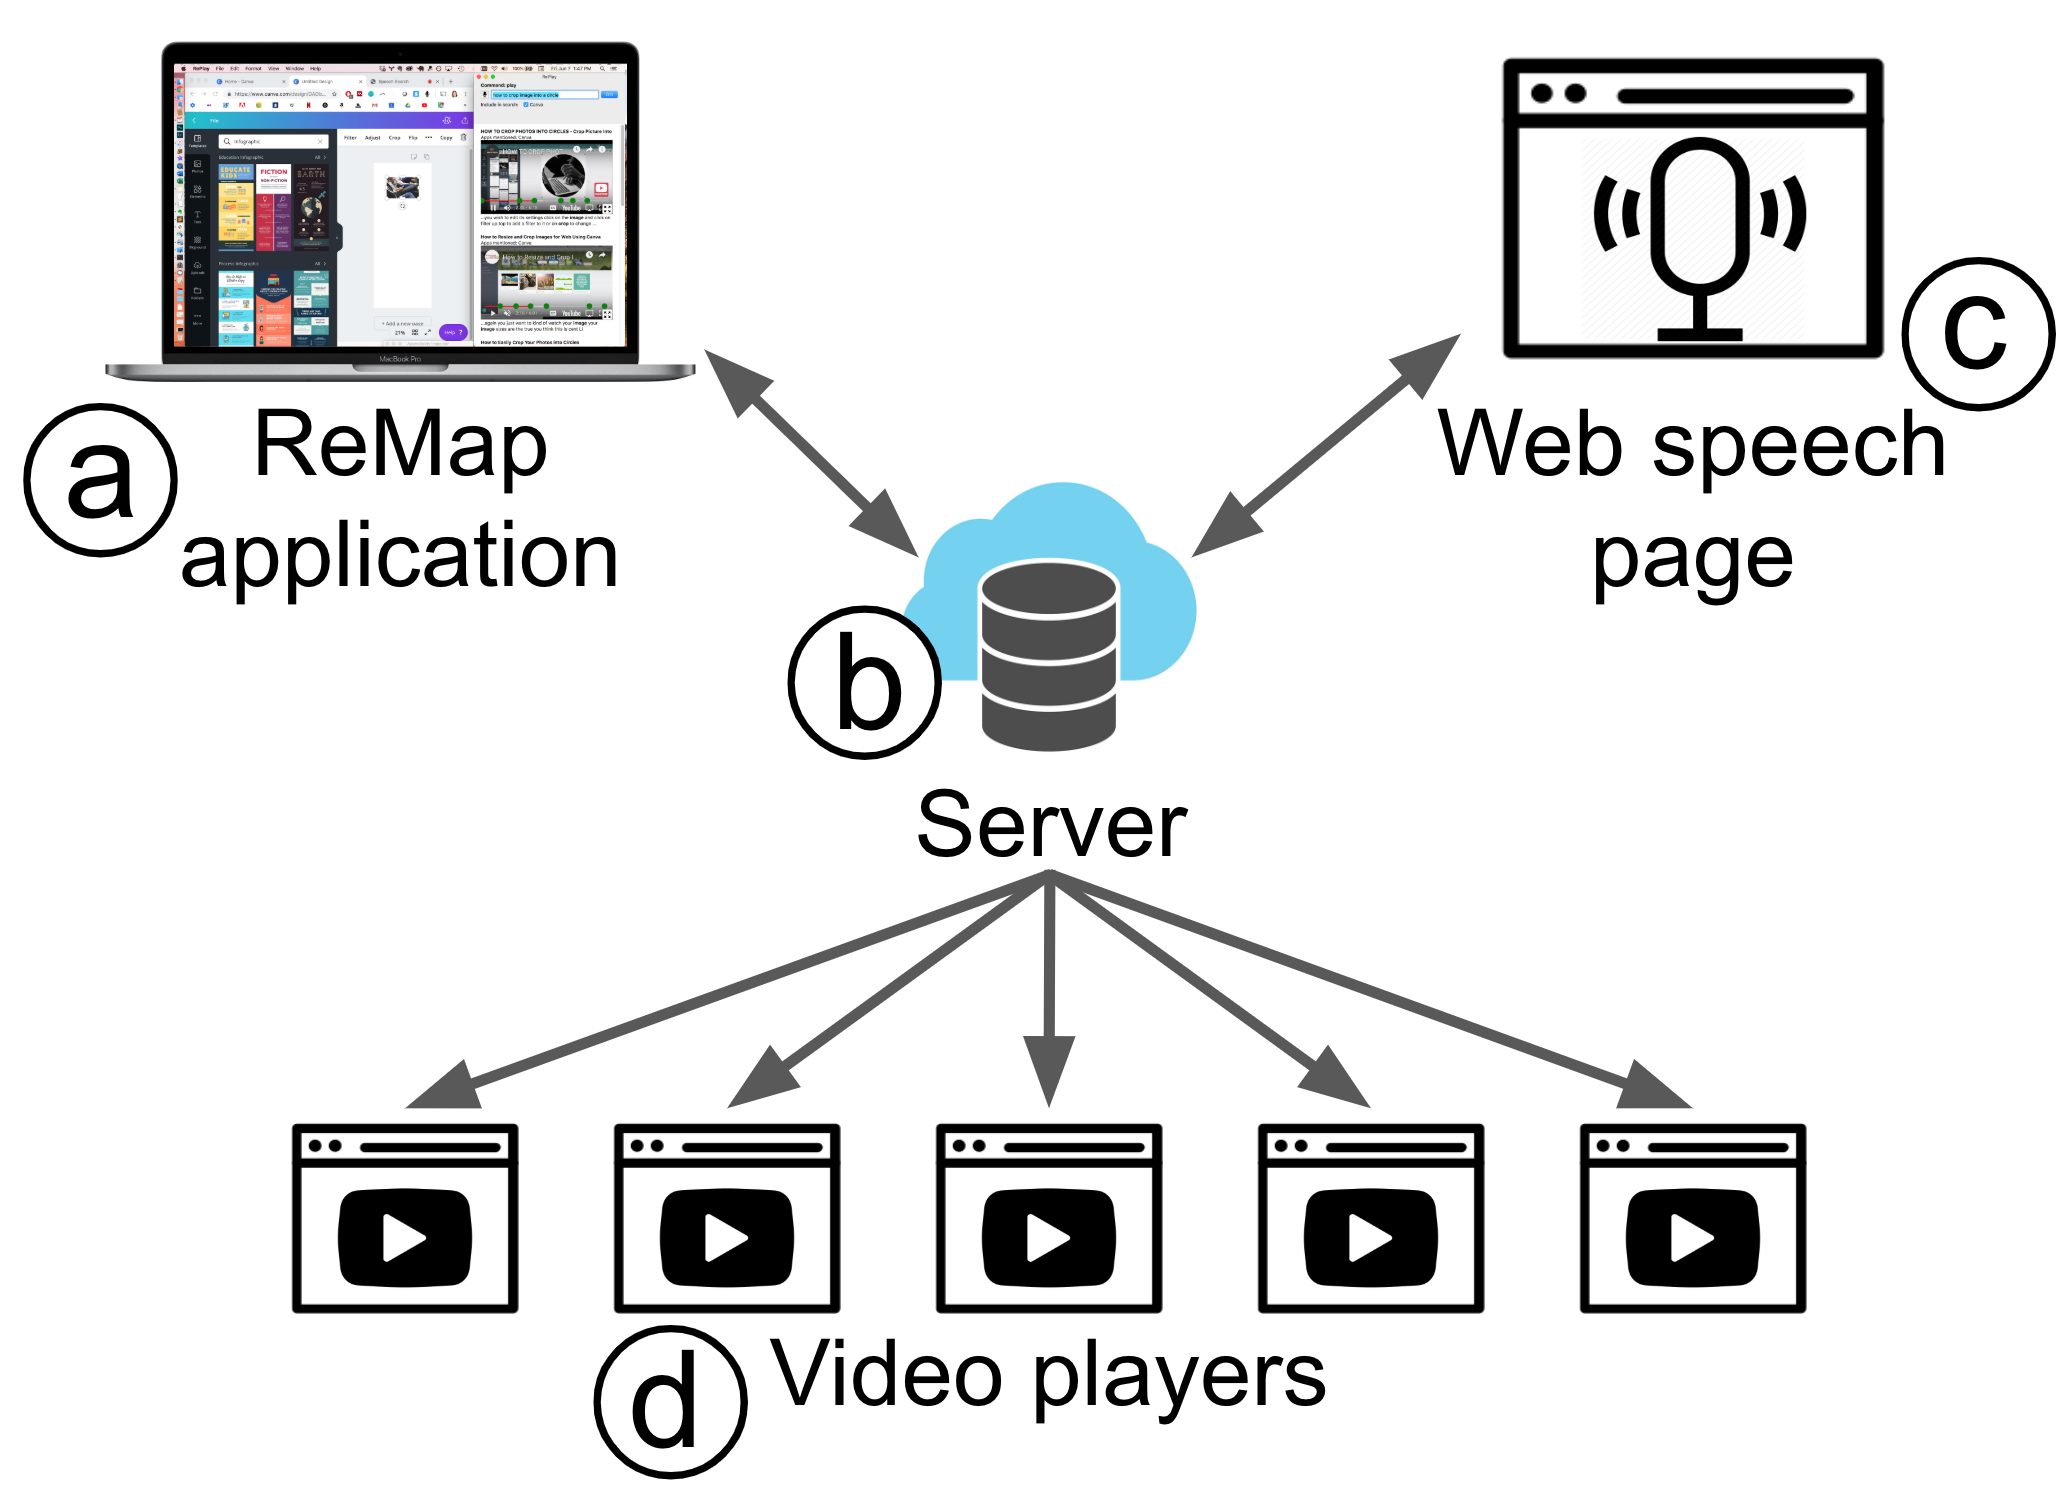
\includegraphics[width=\textwidth]{remap/figures/system.png}
  \caption{The ReMap system architecture. a) ReMap is a MacOS application that uses the Accessibility \textsc{api} to detect user context. b) ReMap connects to a web server, which opens c) a webpage for speech recognition, and d) a video player webpage for each result to embed in ReMap.}~\label{fig:remap_system}
  \vspace{-0.2in}
\end{figure}

\subsection{Navigating video results using speech commands}
The user can speak commands to navigate video results, inspired by Chang \textit{et al.}'s recommendations \cite{Chang2019}. ReMap currently supports the following commands: \textit{``play''} (plays the first or most-recently played video), \textit{``play \{next, previous, last\}''} (plays the next/previous/last video in the list), \textit{``play \{first, second, third, fourth, fifth\} video''}, \textit{``\{next, previous, repeat\} marker''} (skips to the next or previous timeline marker, or re-starts from the current marker), and \textit{``pause''} / \textit{``stop''} (pauses the currently playing video).


\subsection{Implementation}
ReMap is implemented as a MacOS Swift application (\autoref{fig:remap_system}a). It uses socket.io to communicate between the web server and the three client interfaces (the ReMap desktop application, web speech page, and video players). The web server (\autoref{fig:remap_system}b) is implemented in Node.js. The speech engine (\autoref{fig:remap_system}c) uses the Web Speech \textsc{api}, and the video player (\autoref{fig:remap_system}d) uses the YouTube Player \textsc{api} to load and control videos. ReMap generates a unique anonymous user ID for each computer it runs on. When it opens the speech engine and video player webpages, it includes this user ID as a parameter. For video player pages, it also includes that video's index in the result list. The server keeps track of these values for each client page that opens a socket connection, so that it can pass commands it receives to the appropriate client.

The web speech page determines whether a spoken phrase starts with the word \textit{``search''} and if so, sends the rest of the phrase to the server which sends it to the ReMap app as a query. If a phrase matches a video navigation command, the server sends this command to the ReMap app which then determines which video index it applies to, and returns a message to the server telling it which video player to send the command to. If the command was to play a different video than the currently playing video, ReMap also asks the server to pause the currently playing video.

\section{Study: Using ReMap for a Graphic Design Task}
\label{sec:remap_study}
To gain an initial understanding of how people use multimodal search for help, we conducted a think-aloud lab study with thirteen participants. Participants re-created a given design in Canva (\href{https://canva.com}{\nolinkurl{canva.com}}) and used ReMap to search for help when necessary. Overall we found that despite some usability and implementation challenges, multimodal video search was helpful, allowing participants to stay focused on their task while simultaneously searching for help and navigating video resources. 

\subsection{Participants}
Thirteen participants were recruited from mailing lists and flyers at a university. 10/13 participants had at least some experience using voice assistants (\textit{e.g.}, Siri, Amazon echo) (mean = 2.3/5, 1 = never used, 5 = use every day). 6/15 participants had never used Canva before, and only one was very familiar with it (mean = 1.8/5, 1 = never used, 5 = very familiar).

\subsection{Procedure}
Participants were shown two images of an infographic design (\autoref{fig:remap_designs}) and were asked to choose one and re-create it as accurately as possible in Canva without using any of Canva's built-in templates. Participants were asked to use ReMap only (no web search) when they needed to search for help. Participants were given a brief tutorial on how to use ReMap, and were given three example commands to try to ensure they understood how it worked. They were encouraged to use speech as much as possible, but also had the option to type their search queries into ReMap's search field. Participants were asked to think out loud while they worked, and the experimenters captured audio and screen recordings. Participants were scheduled for 2-hour slots and were told to take as much time as they needed. Once they announced they were done (or if 1 hour and 45 minutes had passed), participants were asked a series of interview questions including prompts for Likert-scale responses to understand how they felt the task went, and whether they found ReMap helpful. Participants received a \$30 USD gift card for their time.

\begin{figure}[t!]
\centering
  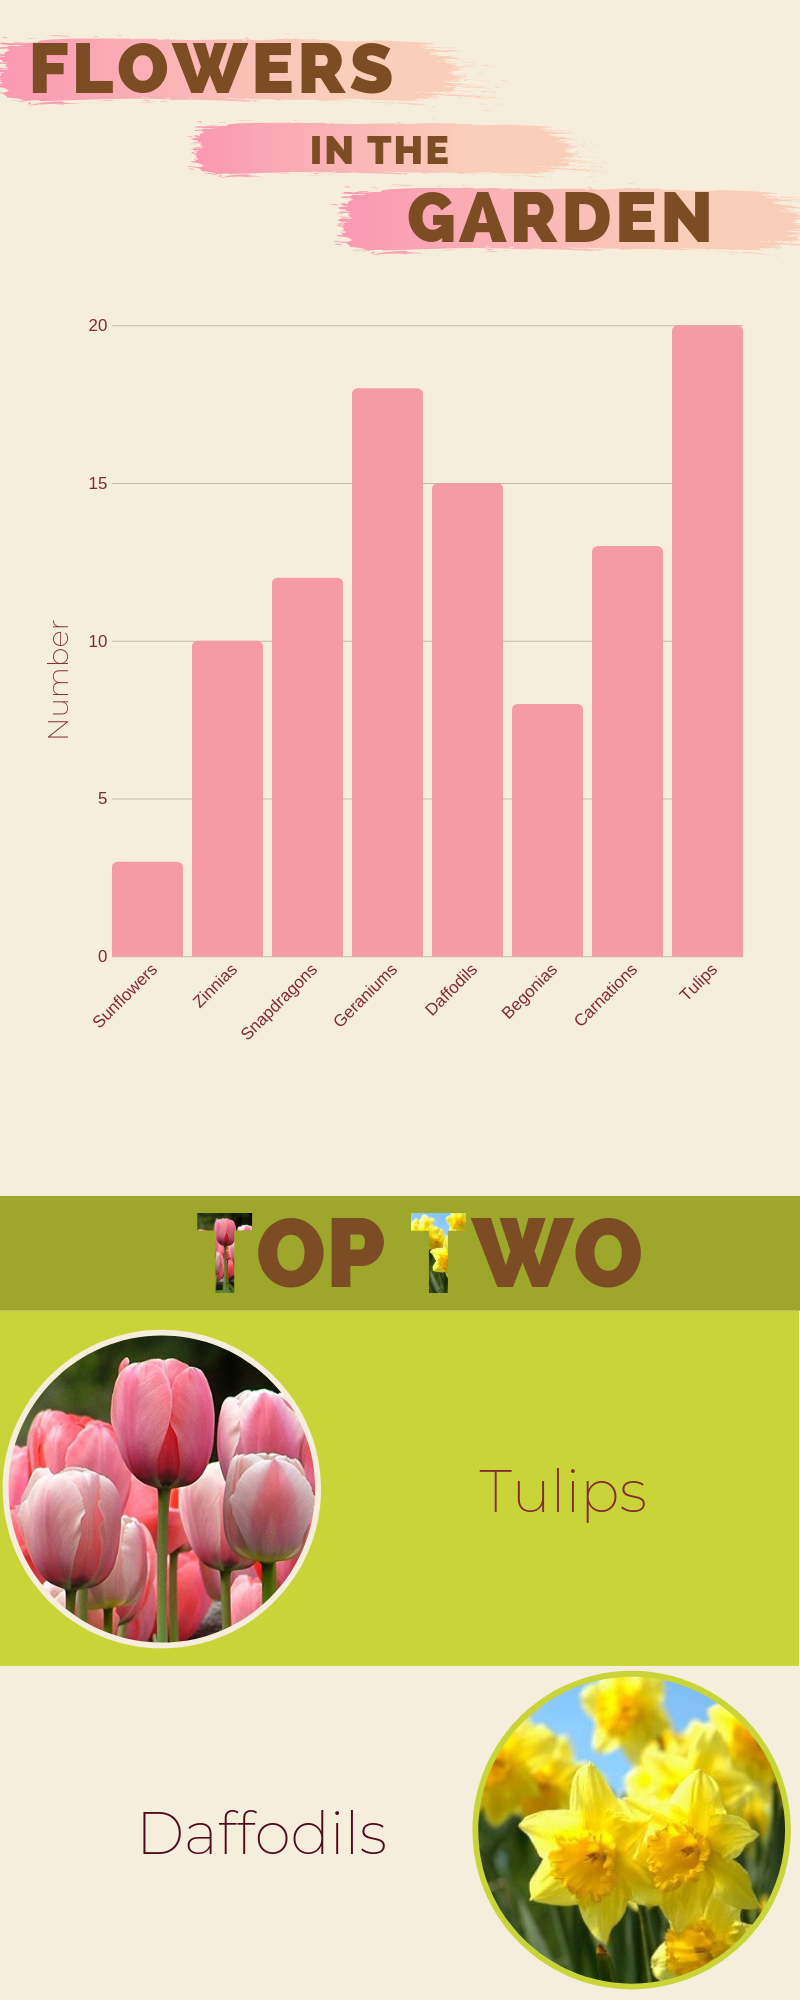
\includegraphics[width=0.3\textwidth]{remap/figures/designA.png}
  \hspace{0.2in}
  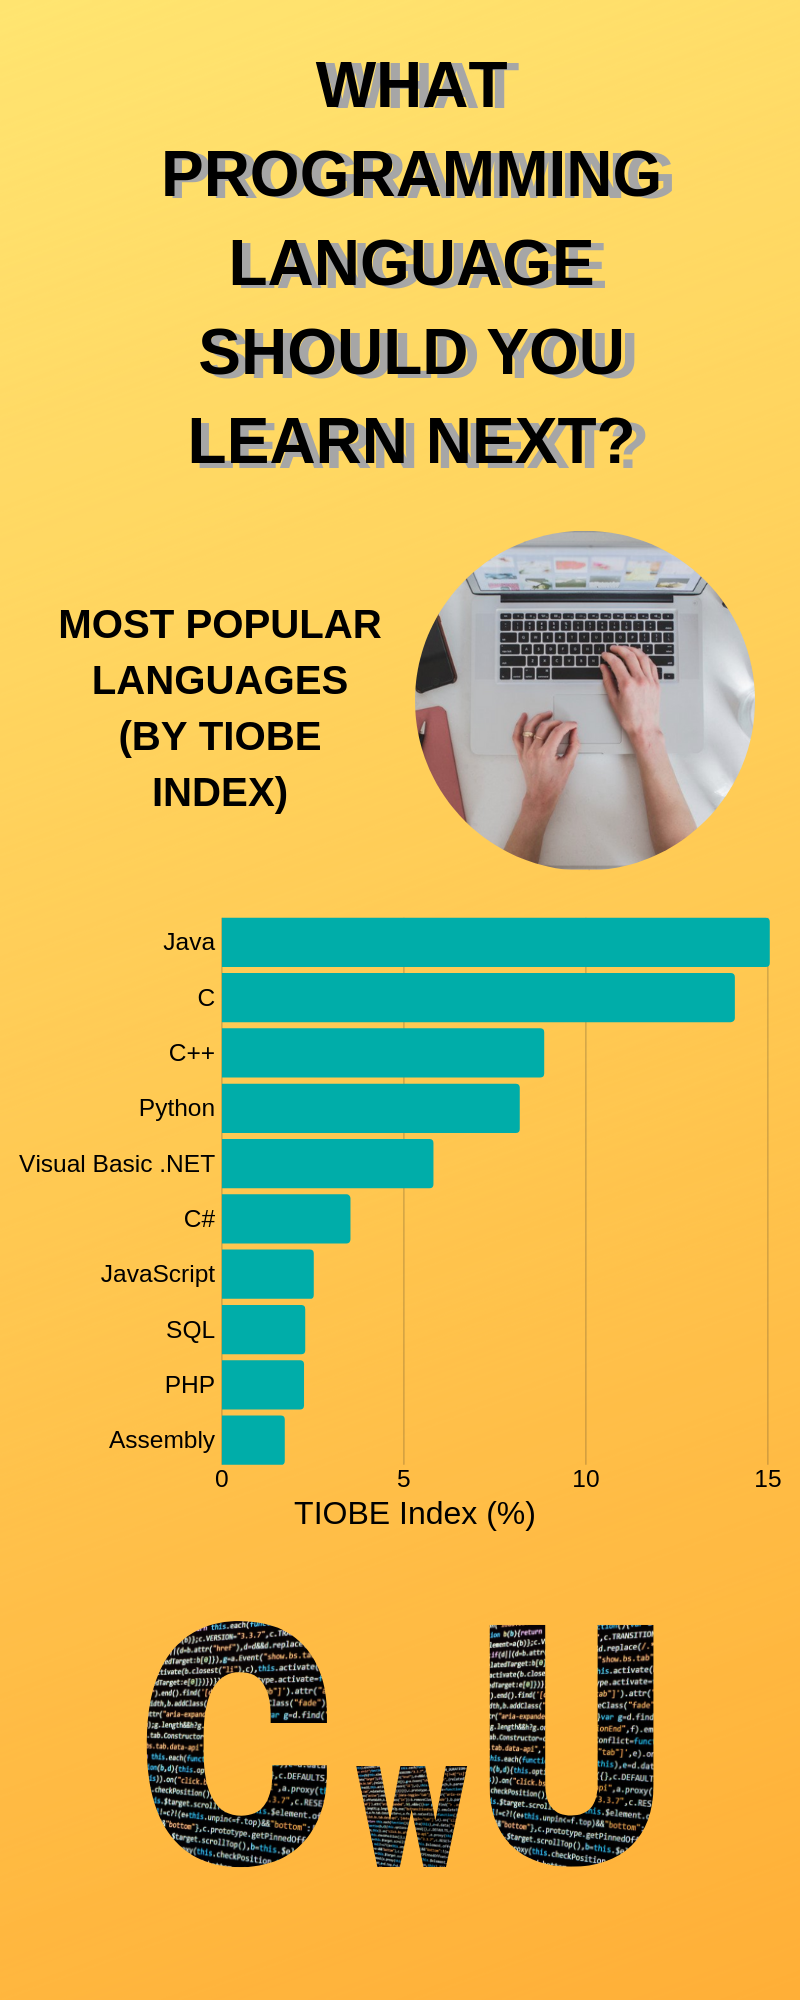
\includegraphics[width=0.3\textwidth]{remap/figures/designB.png}
  \caption{Study participants chose one of the above two infographic designs to re-create in Canva, using ReMap to search for help.}~\label{fig:remap_designs}
\end{figure}

Both infographics were designed to require several operations that are not straightforward in Canva, to increase the likelihood that participants would have to search for help. These included: cropping an image in a circle, masking an image in text, creating a bar chart given a spreadsheet of data, making a swish shape behind text (\autoref{fig:remap_designs} left only) and adding a shadow to text (\autoref{fig:remap_designs} right only).

ReMap's speech recognition requires a clear signal of the user's speech, mostly free of interference from sound output (\textit{i.e.} from videos) or background conversations. We have found commodity headsets to be sufficient, high-quality headsets to be optimal, and built-in laptop microphones insufficient. For the study, participants wore a high-quality headset.

\subsection{Results}
\subsubsection{Search Behaviour}
Participants issued a total of 118 intentional search queries, 111 of which used speech (\autoref{table:remap_results}). An additional 3 queries were issued by mistake (not realizing they had spoken the ``search'' command) and an additional 7 were issued before the participant had finished speaking (because the Web Speech \textsc{api} detected a pause). One participant did not search at all (the same participant that rated their familiarity with Canva as 5/5); the rest issued between 4 and 18 queries each. 

\begin{table}[b!]
\centering
\caption{Summary of each participant’s usage of ReMap. ``\# speech commands'' includes all play, pause, and marker navigation commands. ``\# manual commands'' includes all plays, pauses, seeking along the timeline, and clicking on markers.}~\label{table:remap_results}
\resizebox{1\textwidth}{!}{
\begin{tabular}{lllllllll}
\textbf{} & \textbf{\begin{tabular}[c]{@{}l@{}}Total \#\\ intentional\\ searches\end{tabular}} & \textbf{\begin{tabular}[c]{@{}l@{}}\# accidental or\\ pre-emptive\\ searches\end{tabular}} & \textbf{\begin{tabular}[c]{@{}l@{}}\# intentional\\ speech\\ searches\end{tabular}} & \textbf{\begin{tabular}[c]{@{}l@{}}\# unique\\ videos\\ played\end{tabular}} & \textbf{\begin{tabular}[c]{@{}l@{}}\# speech\\ commands\end{tabular}} & \textbf{\begin{tabular}[c]{@{}l@{}}\# manual\\ commands\end{tabular}} & \textbf{\begin{tabular}[c]{@{}l@{}}\# deictic\\ references\end{tabular}} & \textbf{\begin{tabular}[c]{@{}l@{}}\# successful\\ deictic\\ resolutions\end{tabular}} \\ \hline
P1 & 17 & 1 & 17 & 13 & 41 & 3 & 5 & 1 \\
P2 & 5 & 0 & 5 & 6 & 2 & 93 & 1 & 0 \\
P3 & 13 & 3 & 13 & 7 & 20 & 23 & 10 & 1 \\
P4 & 4 & 0 & 4 & 5 & 14 & 19 & 0 & 0 \\
P5 & 0 & 0 & 0 & 0 & 0 & 0 & 0 & 0 \\
P6 & 8 & 1 & 8 & 5 & 17 & 2 & 0 & 0 \\
P7 & 7 & 1 & 7 & 6 & 24 & 10 & 0 & 0 \\
P8 & 3 & 1 & 3 & 2 & 4 & 1 & 0 & 0 \\
P9 & 8 & 1 & 6 & 6 & 0 & 49 & 0 & 0 \\
P10 & 16 & 0 & 13 & 5 & 10 & 5 & 3 & 0 \\
P11 & 10 & 1 & 10 & 11 & 9 & 51 & 1 & 1 \\
P12 & 11 & 0 & 11 & 4 & 8 & 16 & 1 & 1 \\
P13 & 16 & 1 & 14 & 7 & 18 & 0 & 3 & 2 \\
\textbf{Total} & \textbf{118} & \textbf{10} & \textbf{111} & \textbf{77} & \textbf{167} & \textbf{272} & \textbf{24} & \textbf{6}
\end{tabular}
}
\end{table}

61/118 queries (52\%) were new queries and 34/118 (29\%) were reformulations of previous queries (i.e., rephrasing a query to find better results). The rest were either attempts to fix a failed deictic resolution or fixing a transcription error. 55/118 queries began with either the phrase ``how to'' (42/118), or the phrase ``how do I'' (13/118). 

8/111 speech queries included a speech recognition error. One participant tried to rephrase their query after speaking it twice, leading to long queries with some repetition (\textit{e.g.}, ``resize this without aspect ratio without keeping aspect ratio''). 6 of the 7 non-speech queries were a manual revision of a previous speech query (either error fixes or reformulations). 

7 of 13 participants used deictic references at least once. Only 6 of 24 total deictic references were successfully resolved to a name, mainly because some canvas objects were not recognizable by ReMap (\textit{e.g.,} graphs). 23/24 deictic references referred to objects on the canvas (\textit{e.g.}, text boxes, images, and graphs); the other one referred to a button on the toolbar. This reinforces RePlay's study finding (\autoref{sec:replay_study}) that participants mostly made action-oriented queries, rather than queries about tools or commands, and highlights the need for canvas elements to be recognizable by ReMap.

\subsubsection{Video Navigation Behaviour}
Participants watched a total of 77 videos (\textasciitilde6 videos per participant). In total, participants played videos by clicking on them 60 times, and by saying one of the ``play'' commands 61 times. Participants paused manually 60 times, and via the ``pause'' speech command 46 times. Participants manually seeked to points in the video by dragging on the timeline 124 times, by clicking timeline markers 28 times, and by using the ``next/previous/repeat marker'' commands 60 times. In general, most participants seemed to exhibit a preference for either speech commands or manual navigation of videos (\autoref{table:remap_results}). This highlights the importance of providing both options in a multimodal interface, especially as peoples' preferences and needs may change depending on their task or environment \cite{Reeves2004, LaViolaJr.2014}.

\subsubsection{Participant Feedback}
As \autoref{fig:remap_boxplot} shows, participants generally found all four of ReMap's multimodal features moderately helpful. Based on our observations, most participants used the multimodal features to work and search or watch videos simultaneously. They confirmed this during the post-task interviews, with several participants explicitly mentioning multitasking as a benefit of ReMap's multimodal features. For example, one participant described how ReMap helped them be more efficient than their current strategies for help-seeking:

\begin{quote}
\textit{``When I'm designing graphics myself sometimes I get stuck, so I will have to stop everything and go to YouTube or Google to find it, but if I'm able to work while listening or ... watching it on the side, through voice, I think it will help with efficiency ... `cause at one point I was able to ... move the things around while listening for the things I need.''} --- P4
\end{quote}

\begin{figure}[t!]
\centering
  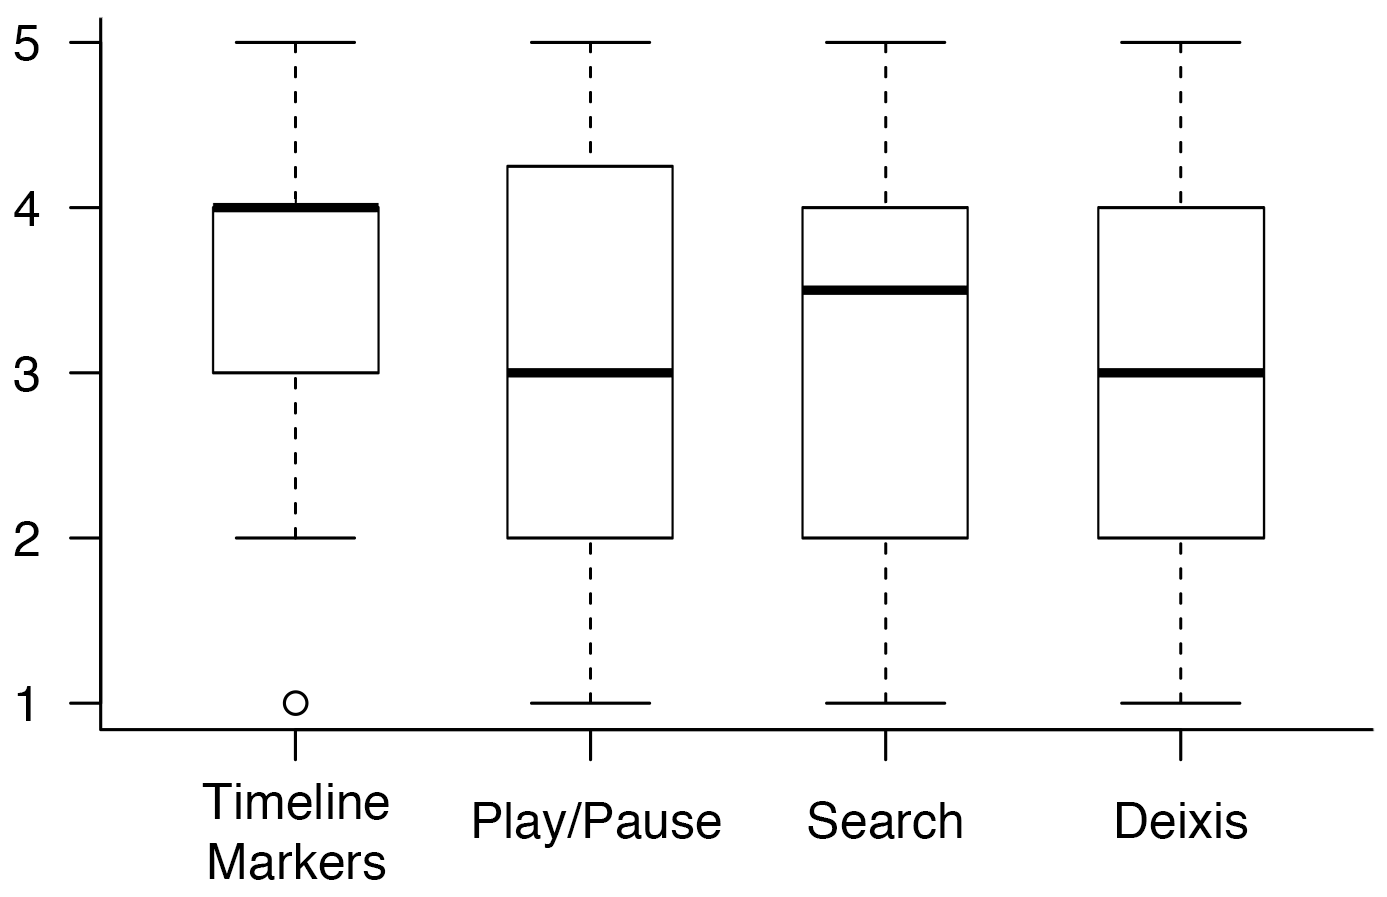
\includegraphics[width=0.7\textwidth]{remap/figures/boxplot.png}
  \caption{Distribution of participants' ratings of ReMap’s multimodal features. 1 = not helpful at all, 5 = very helpful. Bold lines represent median values, and boxes illustrate interquartile ranges. }~\label{fig:remap_boxplot}
\end{figure}

\textbf{Timeline markers:}
Navigating the timeline markers was rated as the most helpful multimodal feature on average, and was the most common answer participants gave when asked what their favorite feature of ReMap was. This is mainly because it supported participants in multitasking:

\begin{quote}
\textit{``I ... found it helpful because while it was switching I could multitask, and I could just tell it `hey, go to the next marker', and then I would try to do stuff on my own on the side until it plays.''} --- P6
\end{quote}

\begin{quote}
\textit{``If I couldn't use speech then i would have to ... actually click on the videos, but since I'm already working on this part of the screen, then [speech is] just more convenient.''} --- P7
\end{quote}

The markers themselves were useful (as the RePlay study (\autoref{sec:replay_study}) also showed) as they provided a shortcut to potentially relevant moments in the video. The speech commands for skipping between them made it easy for participants to back-up or fast-forward the video to a reasonable point. This is easier than having to specify a specific time interval to skip between, which Chang et al. \cite{Chang2019} showed can be difficult for people following along with video tutorials. However, some participants did mention that they preferred using the mouse to hover over markers before selecting them, so they could see the caption previews (\autoref{fig:replay-green_markers}): \textit{``I don't really know what they are until I scroll over them''} (P11).

\textbf{Play/pause:}
Some participants also found speech for playing and pausing videos to be helpful, as it allowed them to follow along with videos at their own pace, which prior work has also demonstrated the importance of \cite{Chang2019, Pongnumkul2011}.

\begin{quote}
\textit{``It's really helpful because if I hear the info I want and I'm kind of following along I can pause it, take the instructions, apply it, and then ... continue watching ... without having to stop the fluidity of work.''} --- P8
\end{quote}
\begin{quote}
\textit{``It was nice to be able to keep track of the video in the background while also starting to think through the next thing and having my focus on the other window.''} --- P13
\end{quote}

Other participants preferred using the mouse to play and pause the videos as they felt it was just as fast or easy, and didn't require them to remember the correct wording of the commands.

\textbf{Speaking query:}
Many participants found it helpful to speak their query out loud rather than type it, as it also supported multitasking and allowed them to stay focused on the task in Canva. Some also said that it was easier or faster than typing. However, some other participants found it more difficult to speak their query, as they didn't always know exactly what to say when they started, and they were not used to speaking out loud to search. As P13 described, \textit{``I had a lot of trouble getting my queries totally straight or thought out in my head before starting to speak them.''} One common difficulty encountered with ReMap's implementation was that it would cut off a participant's query and issue the search before they were done speaking, often because they paused slightly while thinking of what to say. This happened 7 times and was due to the Web Speech \textsc{api} prematurely detecting the end of a phrase. As one participant described, it made them feel rushed to finish speaking:

\begin{quote}
\textit{``It kept rushing me to think about what I wanted to search for ... Usually when I search by typing, I type out half of what I want and then think about ... what to type for the rest, whereas here as soon as i said `how to add' I had to immediately know what I was searching.''} --- P6
\end{quote}

\textbf{Deixis:}
The 7 participants who attempted using deixis in their queries mostly found it helpful, although many noted that it needed some improvement to be useful. It helped participants include words they didn't know in their queries and was often easier and faster than saying or typing the words explicitly. However, it is likely most helpful in cases where users do not know the terminology, and Canva's interface has a relatively straightforward vocabulary. For example, P1, who rated their prior experience with Canva as 1.75/5, said \textit{``it might be more helpful for things that you don't know the exact terminology for, but I think I knew some of the terminology so just saying it felt faster.''}

ReMap's deictic resolution also suffered some implementation and usability challenges: deictic references were only successfully resolved 25\% of the time, usually due to objects on the canvas not being recognized by the Accessibility \textsc{api}. Two participants also pointed out that their eyes naturally went to the search field where their query was appearing while they spoke it, which made it difficult to look at Canva instead to reference elements: \textit{``even though i was trying to click here i was focusing on [the search field]''} (P9).

\textbf{Overall:}
Finally, when asked if participants could see themselves using ReMap in their daily lives, 9 participants said yes (3 saying for certain tasks only, and 2 saying if the technology improved first). The 4 participants who said no shared reservations about using speech in public or around people, and some said they simply prefer typing.

\section{Discussion / Challenges}
\subsection{Implementation Challenges}
- having to be a macos app because accessibility, but no good speech so having to use web speech api
- accessibility in general not super good --> deictic failed a lot
\subsection{Usability Challenges}
- searching unintentionally (midas touch)
- or not listening when keyword was misheard
- cutting off before they were done talking
- correcting query is hard, mostly resort to typing or people would repeat themselves but system isn't that smart
- showing query as they spoke might have been distracting - they weren't looking at the task anymore
\subsection{Potentail IMprovements / future exploration to do}
- compare keyword to search vs. button / keyboard shortcut
- let user decide when done talking (adds extra step but could prevent errors)
- explore how to correct queries (existing work?) using speech -- detect if they repeat themselves and go with the second version, or suport things like "x instead of y"
- compare not showing query (just listening) vs. showing it
- other ways to do deictic -- computer vision like prefab?
- higher level -- do people really want deictic? is it useful? most queries (as we found with replay too) were not about tools so being able to refer to them isn't that useful, and other things (like objects on the canvas) people mostly know what they are called so it doesn't save much time
- deictic may be more useful for issuing commands or sending questions to people / posting in forums
\section{Conclusion}
ReMap introduces multimodal interaction for quick, in-context help-seeking by leveraging the strengths of multiple modalities. Users can search for videos using speech, use deixis to include application-specific terminology, and use speech to navigate videos. An initial study showed that ReMap helps people stay focused on their task while navigating help resources, and highlighted several important challenges with multimodal search. 
%Future work should explore how to make deictic resolution more robust and further lower the barrier to searching in context.

RePlay and ReMap demonstrated how bringing learning videos into the user's context can help people find procedural help while working toward a specific desired outcome. The next chapters in this dissertation break apart the goals of \textit{process} and \textit{outcome}, exploring how contextual systems can support users who desire only one or the other.

\section{Acknowledgements}
This chapter, in part, is currently being prepared for submission for publication of the material. C. Ailie Fraser, Julia M. Markel, N. James Basa, Mira Dontcheva, and Scott Klemmer. The dissertation author was the primary investigator and author of this material.



%% APPENDIX
\appendix
\chapter{Final notes}
What to do about things \cite{Martin_1983}.  What did he say \cite{Rilling_Insel_1999}.
  Remove me in case of abdominal pain.



%% END MATTER
% \printindex %% Uncomment to display the index
% \nocite{}  %% Put any references that you want to include in the bib 
%               but haven't cited in the braces.
\bibliographystyle{SIGCHI-Reference-Format}  %% This is just my personal favorite style. 
%                              There are many others.
%\setlength{\bibleftmargin}{0.25in}  % indent each item
%\setlength{\bibindent}{-\bibleftmargin}  % unindent the first line
%\def\baselinestretch{1.0}  % force single spacing
%\setlength{\bibitemsep}{0.16in}  % add extra space between items
\bibliography{references}  %% This looks for the bibliography in references.bib 
%                          which should be formatted as a bibtex file.
%                          and needs to be separately compiled into a bbl file.
\singlespace  %to force bibilography environment to use single spacing for each entry 
              %double spacing between entries remains
\end{document}

